\documentclass[russian,10pt]{article}

\usepackage[intlimits]{amsmath}
\usepackage{amsthm,amsfonts}
\usepackage{amssymb}
\usepackage{mathrsfs}
%\usepackage{graphicx}
\usepackage[final]{graphicx,epsfig} 
\usepackage{longtable}
\usepackage{indentfirst}
\usepackage[utf8]{inputenc}
\usepackage[T2A]{fontenc}
\usepackage[russian,english]{babel}
\usepackage[usenames]{color}
\usepackage{esint}
\usepackage{bbm}
\usepackage{styles/mystyle}


\pdfpagewidth 14cm
\pdfpageheight 20cm

\textwidth 11cm
\textheight 16.5cm
\oddsidemargin 1.5cm % 1.84cm
\topmargin 1.5cm % 1.8cm
\footskip 1cm

\hoffset -1in
\voffset -1in
\headheight 0pt
\headsep 0pt

\hyphenpenalty=300
%\tolerance=800
\binoppenalty=10000

\clubpenalty=10000 \widowpenalty=10000  % подавление "висячих строк"
\tolerance=2000  % терпимость к жидким строкам
\righthyphenmin=2  % минимальное число символов при переносе* 

% Adjust first page number according to real document position in the book.
\setcounter{page}{1}

% Dot after section number
\makeatletter
% In section title
\def\@seccntformat#1{\csname the#1\endcsname.\quad}
\makeatother

%\tolerance = 2000

% To place author above title
\def\maketitle{
  \begin{center}


\thispagestyle{empty} 
\begin{center}

МИНИСТЕРСТВО ОБРАЗОВАНИЯ И НАУКИ \\
РОССИЙСКОЙ ФЕДЕРАЦИИ \\

 $ $ \\

Московский физико-технический институт \\
(государственный университет) \\
 
  $ $ \\ $ $ \\ $ $ \\
  $ $ \\
  $ $  \\
\smallskip
\smallskip
\premierAuthors, \\
\autresAuthors \\
 
 $ $ \\ $ $ \\
 
\textbf{СТОХАСТИЧЕСКИЙ АНАЛИЗ \\ В ЗАДАЧАХ} \\
 
 $ $ \\
  $ $ \\
  $ $ \\
Учебно-методическое пособие \\
 
  $ $ \\ $ $ \\ $ $ \\ $ $ \\
  \smallskip
   Часть 2
 $ $ \\ $ $ \\ $ $ \\ $ $ \\ $ $ \\ $ $ \\
 
Москва--Долгопрудный 2015


\end{center}

\newpage
  \end{center}
}

\renewcommand{\refname}{Литература}

%\sloppy
%\DeclareGraphicsRule{*}{eps}{*}{}
\DeclareMathOperator{\diam}{diam}

\graphicspath{{images/}}
\newcommand{\imgh}[3]{\begin{figure}[!h]\center{\includegraphics[width=#1]{#2}}\caption{#3}\label{Fig:#2}\end{figure}}

% Perfectly typesetted tilde for url links.
%\def\urltilde{\kern -.15em\lower .7ex\hbox{\~{}}\kern .04em}

\addto{\captionsrussian}{
	\renewcommand{\proofname}{\bf Решение}
}

\usepackage{wasysym}
\usepackage{verbatim}

\makeatletter
\g@addto@macro\th@definition{\thm@headpunct{.}}
\makeatother
\theoremstyle{definition}


%\newtheorem{problem}{\noindent\normalsize\bfЗадача \No\!\!}
\newtheorem{problem}{\noindent\normalsize\bf{}}[section]

\renewcommand{\theproblem}{\noindent\arabic{problem}}

\newtheorem*{example}{\noindent\normalsize\bf{}Пример}
\newtheorem*{definition}{\noindent\normalsize\bf{}Определение}
\newtheorem*{remark}{\noindent\normalsize\bf{}Замечание}
\newtheorem{theorem}{\noindent\normalsize\bf{}Теорема}
\newtheorem*{lemma}{\noindent\normalsize\bf{}Лемма}
\newtheorem*{suite}{\noindent\normalsize\bf{}Следствие}


\newtheorem*{ordre}{\noindent\normalsize\bf{}Указание}

\newenvironment{solution}{\begin{proof}\vspace{1em}} {\end{proof} \vspace{2em}}

\newcommand{\atoc}[1]{\addtocontents{toc}{\hspace{0.4\linewidth}#1\par}}

%\newcommand{\fixme}[1]{\textcolor{red}{\noindent\normalsize\frownie{}[#1]}} %for displaying red texts

\newcommand{\fixme}[1]{}


\usepackage{enumitem}

\RequirePackage{enumitem}
\renewcommand{\alph}[1]{\asbuk{#1}} % костыль для кирилической нумерации 

\setenumerate[1]{label=\alph*), fullwidth, itemindent=\parindent, 
  listparindent=\parindent} 
\setenumerate[2]{label=\arabic*), fullwidth, itemindent=\parindent, 
  listparindent=\parindent, leftmargin=\parindent}

\newcommand{\rg}{\ensuremath{\mathrm{rg}}}
\newcommand{\grad}{\ensuremath{\mathrm{grad}}}
\newcommand{\diag}{\ensuremath{\mathrm{diag}}}
\newcommand{\const}{\ensuremath{\mathop{\mathrm{const}}}\nolimits}
\newcommand{\Var}{\ensuremath{\mathop{\mathbb{D}}}\nolimits}
\newcommand{\Exp}{\ensuremath{\mathrm{{\mathbb E}}}}
\newcommand{\PR}{\ensuremath{\mathrm{{\mathbb P}}}}
\newcommand{\Be}{\ensuremath{\mathrm{Be}}}
\newcommand{\Po}{\ensuremath{\mathrm{Po}}}
\newcommand{\Beta}{\ensuremath{\mathrm{Beta}}}
\newcommand{\Dir}{\ensuremath{\mathrm{Dir}}}
\newcommand{\Bi}{\ensuremath{\mathrm{Bi}}}
\newcommand{\Ker}{\ensuremath{\mathrm{Ker}}}
\newcommand{\Real}{\ensuremath{\mathrm{Re}}}
\newcommand{\Lin}{\ensuremath{\mathrm{Lin}}}
\newcommand{\Gl}{\ensuremath{\mathrm{Gl}}}
\newcommand{\mes}{\ensuremath{\mathrm{mes}}}
\newcommand{\cov}{\ensuremath{\mathrm{cov}}}
\newcommand{\I}{\ensuremath{\mathrm{I}}}
\newcommand{\N}{\ensuremath{\mathcal{N}}}
\newcommand{\KL}{\ensuremath{\mathcal{KL}}}
\newcommand{\Star}{\hspace{-6pt}*\hspace{3pt}}
\newcommand{\DStar}{\hspace{-6pt}**\hspace{3pt}}
\newcommand{\Nbb}{\mathbb{N}}

\usepackage{watermark}
\thiswatermark{\put(-100,-550){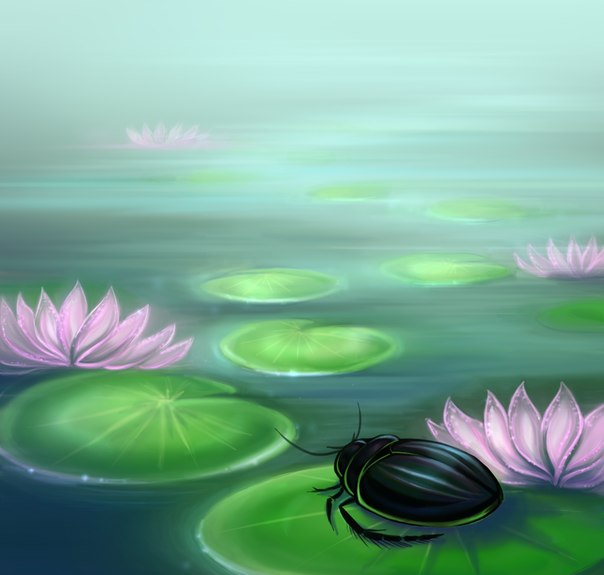
\includegraphics[scale=0.8]{images/guk.jpg}} }

\usepackage{url}
\makeatletter
\g@addto@macro{\UrlBreaks}{\UrlOrds}
\makeatother

\begin{document}

\selectlanguage{russian}

\maketitle

\atoc{Часть 1}

\thispagestyle{empty} 

УДК 519.21
 
 $ $ \\ $ $ \\
 
\premierAuthors, \autresAuthors. Стохастический анализ в задачах: Учебно-методическое пособие. Часть 1 / МФТИ. М.--Д., 2015, изд. 3-е, доп.

$ $ \\ 
 
\begin{abstract}

Содержит программу, список литературы и задачи одноименного курса, читаемого сотрудниками кафедры Математических основ управления студентам факультета управления и прикладной математики Московского физико-технического института. Задачи могут быть использованы в качестве упражнений на семинарских занятиях, сдачах заданий, экзаменах, а также при самостоятельном освоении курса. В новое издание добавлен ряд задач, отражающих также опыт преподавания вероятностных дисциплин в Независимом московском университете и опыт наших коллег из ПреМоЛаб МФТИ, преподающих вероятностные дисциплины в ведущих научных центрах Германии и Франции. Данный сборник задач разрабатывался с учетом направлений подготовки: студентов МФТИ, студентов НМУ, магистров факультета Компьютерных наук ВШЭ и магистров факультета Прикладной математики БФУ им. И.~Канта.  

 $ $ \\ $ $ \\ $ $ \\ $ $ \\ $ $ 

\noindent рецензенты: д.ф.-м.н. А.В. Колесников \\
\noindent проф. Факультета математики НИУ ВШЭ \\
\noindent д.ф.-м.н. А.Н. Соболевский \\ 
\noindent проф. Независимого московского университета, \\ зам. директора ИППИ РАН 

\end{abstract}


  
 \newpage 


\thispagestyle{empty} 
\begin{center}

{ОБЯЗАТЕЛЬНАЯ ЧАСТЬ ПРОГРАММЫ УЧЕБНОГО КУРСА  \\ 
«Теория вероятностей»  }
 
\end{center}
 
 {\small
 
Интуитивные предпосылки теории вероятностей. Множество элементарных исходов опыта, событие. Классическое и статистическое определение вероятности. Математическое определение вероятности. Алгебра и сигма-алгебра событий, минимальная сигма алгебра. Аксиомы теории вероятностей и следствия из них. Вероятностное пространство.

Теорема непрерывности вероятности. Теорема сложения вероятностей. Зависимые и независимые события. Условная вероятность события. Формула полной вероятности. Формула Байеса. Леммы Бореля--Кантелли. Закон ``0-1'' Колмогорова.

Случайная величина как измеримая функция. Функция распределения случайной величины. Дискретные и непрерывные случайные величины. Плотность распределения вероятностей. Формула включений-исключений.

Конкретные распределения случайных величин. Схема Бернулли, геометрическое и биномиальное распределение. Простейший поток событий и распределение Пуассона. Показательное, равномерное, нормальное, log-нормальное и отрицательно-биномиальное распределения. Бета-распределение и гамма-распределение.

Случайный вектор. Функция распределения случайного вектора. Зависимые и независимые случайные величины, условные законы распределения. Функции случайных величин. Невырожденное функциональное преобразование случайного вектора.
Интеграл Стилтьеса. Математическое ожидание и дисперсия случайной величины. Моменты случайной величины. Условное математическое ожидание. Корреляционная матрица случайного вектора. Коэффициент корреляции двух случайных величин.

Характеристическая функция и ее свойства. Связь моментов случайной величины с ее характеристической функцией. Разложение характеристической функции в ряд.
Сходимость последовательностей случайных величин с вероятностью единица (почти наверное), порядка $p$ (в среднем квадратичном), по вероятности, по распределению. Соотношение между различными типами сходимости. 

Неравенство Чебышева. Закон больших чисел. Критерий Колмогорова. Теоремы Хинчина и Чебышева.  Усиленный закон больших чисел. Теорема Колмогорова и Бореля. Оценивание скорости сходимости частоты к вероятности в схеме Бернулли. Неравенство Бернштейна. 

Интегральная и локальная теоремы Myавра--Лапласа. Дискретная поправка. Теорема Линдберга. Центральная предельная теорема для одинаково распределенных случайных величин. Центральная предельная теорема в форме Натана. Условие Ляпунова. Теорема Гливенко.
}


\newpage

\section{Введение}

В основу предлагаемого сборника задач по теории вероятностей положены задачи (в том числе повышенной сложности), предлагавшиеся в разные годы студентам факультета управления и прикладной математики (ФУПМ) МФТИ и Независимого московского университета на семинарах, сдачах заданий и экзаменах. Главными отличительными особенностями пособия являются: а) широкий спектр представленного материала, б) отражение ряда современных направлений развития теории вероятностей и в) нацеленность на приложения.

По замыслу авторов, предлагаемый сборник задач отчасти демонстрирует роль курса как “вероятностного фундамента” для ряда других дисциплин: прикладной статистики, стохастических дифференциальных уравнений, эффективных алгоритмов, экспериментальной экономики (финансовой математики) и др. Несмотря на широкий спектр представленных тем, основной  акцент делается на формирование у читателей геометрической интуиции, восходящей к Пуанкаре, которая позволяет с единых позиций понять многообразие асимптотических результатов стохастической теории как проявление одного общего принципа концентрации меры. 

Большое внимание в сборнике уделяется различным приемам доказательства предельных теорем – асимптотических результатов теории вероятностей. Для этого прежде всего используется аппарат производящих функций и теории функций комплексного переменного.

Более половины представленных в сборнике задач не являются стандартными. Для таких задач даны указания, комментарии (замечания), ссылки на публикации. 

Желающих более глубоко изучить представленные темы отсылаем к списку литературы, приведенному в конце сборника задач. 

Следует отметить, что за последние десять лет заметно возросло значение для выпускников Физтеха глубоких знаний вероятностных дисциплин. Это обусловлено множеством причин.

Прежде всего, это вызвано широким распространением задач анализа больших массивов данных (machine learning, data mining). Подтверждением служит взаимная востребованность студентов ФУПМ и Школы анализа данных компании Яндекс, большая популярность среди  студентов ФУПМ кафедры интеллектуальных систем (заведующий кафедрой член-корреспондент РАН К.В. Рудаков, Вычислительный центр РАН) и кафедры предсказательного моделирования (заведующий кафедрой академик РАН А.П. Кулешов, Институт проблем передачи информации РАН). 
%Во многом именно для таких студентов и написаны разделы \ref{bayes}, \ref{zb4}, \ref{MK}, \ref{stats}, ССЫЛКА[Оптимизация и стохастика]. %3 – 6, 9, 10.

Другая не менее важная причина -- разработка эффективных (приближенных, рандомизированных) алгоритмов решения сложных задач. 
%Этому посвящены разделы \ref{MK}, \ref{information}, \ref{CS}, ССЫЛКА[Оптимизация и стохастика].
Сложно, например, представить себе современного специалиста по моделированию, который бы не использовал методы Монте-Карло. Также сложно представить себе специалиста в области computer science, которому не приходилось бы применять рандомизированные алгоритмы и подвергать алгоритмы вероятностному анализу (например, для оценки сложности в среднем). 

Еще одна причина  связана с тем, что приложение вероятностных методов к анализу и разработке экономических моделей для части студентов ФУПМ является фундаментом в работе на базовых кафедрах. Например, заведующие базовыми кафедрами ФУПМ член-коррерспондент РАН И.Г. Поспелов (Вычислительный центр РАН) и  член-коррерспондент РАН Ю.С. Попков (Институт системного анализа РАН) активно работают в направлении разработки вероятностных моделей экономических агентов и вероятностного анализа агломерационных моделей. %Этому посвящен раздел ССЫЛКА[Марковские модели макросистем].

Наконец, можно заметить, что задачи анализа больших компьютерных, социальных, транспортных сетей в последнее время выходят на передний план во многих приложениях. Огромную роль в изучении таких сетей играют вероятностные модели, некоторые из которых будут приведены в предлагаемом сборнике задач. 
%Разделы \ref{hard}, \ref{genF}, \ref{combinatorics}, ССЫЛКА[Марковские модели макросистем] сборника посвящены изучению подобных сетей, в частности, различным предельным переходам.

Важную роль в подготовке настоящего сборника задач сыграла Лаборатория структурных методов анализа данных в предсказательном моделировании (ПреМоЛаб), открытая на базе ФУПМ МФТИ в 2011 году. В частности, благодаря этой лаборатории, у студентов есть возможность посмотреть на сайте www.mathnet.ru, www.premolab.ru (семинары: Стохастический анализ в задачах, Математический кружок и др.) видеозаписи выступлений ведущих ученых, посвященные ряду нестандартных задач из этого сборника. 

Мы благодарны нашим коллегам Д.В. Беломестному, Я.И.~Белопольской, М.Л.~Бланку, Н.Д.~Введенской, В.В.~Веденяпину, Д.П.~Ветрову, А.М.~Вершику, К.В.~Воронцову, В.В.~Вьюгину, В.В.~Высоцкому, А.В.~Калинкину, М.Н.~Вялому, М.С.~Гельфанду, Э.Х.~Гимади, Г.К.~Голубеву, А.Б.~Дайняку, П.Е.~Двуреченскому, Н.Х.~Ибрагимову, М.И.~Исаеву, Г.А.~Кабатянскому, А.В.~Колесникову, А.В.~Леонизову, Г.~Лугоши, Ю.В.~Максимову, В.А.~Малышеву, В.Д.~Мильману, В.В.~Моттлю, Т.А.~Нагапетяну, А.В.~Назину, Ю.Е.~Нестерову, А.С.~Немировскому, В.И.~Опойцеву, Ф.В.~Петрову, С.А.~Пирогову, Б.Т.~Поляку, И.Г.~Поспелову, А.М.~Райгородскому, В.Н.~Разжевайкину, М.А.~Раскину, В.Г.~Редько, A.Е.~Ромащенко, А.В. Савватееву, А.Н.~Соболевскому, А.~Содину, В.Г.~Спокойному, Й.~Стоянову, У.~Сэндхольму, С.П.~Тарасову, И.О.~Толстихину, М.Ю.~Хачаю, О.С.~Федько, Ю.А.~Флёрову, А.X.~Шеню, оказавшим заметное влияние на формирование различных разделов этого учебного пособия, и А.А. Шананину, во многом способствовавшему развитию на ФУПМ базового цикла вероятностных дисциплин. Также отметим большую помощь старшекурсников, аспирантов ФУПМ и участников нашего стохастичексого семинара в НМУ и Физтехе в вычитке этого сборника задач (в особенности, Д.~Бабичева, А.~Балицкого, Ф.~Гончарова, Ю.~Дорна, Е.~Клочкова, А.~Макарова, Е.~Молчанова, Н.~Животовского, М.~Панова, Л.~Прохоренкову(Остроумову), А.~Суворикову, Д.~Петрашко, М.~Широбокова).

\begin{center}
\textbf{
Список обозначений
}
\end{center}

\noindent $\langle \Omega, \mathcal{F}, \PR \rangle$ -- вероятностное пространство ($\Omega$ -- множество исходов, $\mathcal{F}$ -- $\sigma$-алгебра, $\PR$ -- вероятностная мера); \\
$p(x), \; f(x), \; f_X(x)$ -- плотность распределения случайной величины $X$;
$\Exp X$ -- математическое ожидание случайной величины $X$; \\
$\Exp_p X$ -- математическое ожидание $X$ с плотностью распределения $p$; \\
$\Exp_\PR X$ -- математическое ожидание $X$ по мере $\PR$; \\
$\Var X$ -- дисперсия случайной величины $X$; \\
$\N(m,\sigma^2)$ -- нормальное распределение; \\
$\Po(\lambda)$ -- распределение Пуассона; \\
$\Dir(\alpha_1,...,\alpha_n)$ -- распределение Дирихле;\\
$\Beta(\alpha,\beta)$ -- бета-распределение;\\
$\Be(p)$ -- распределение Бернулли; \\
$R[a,b], [a,b]$ -- равномерное распределение; \\
$\Phi(x)$ -- функция стандартного нормального распределения $\N(0,1)$; \\
$\mathrm{Exp}(x)$ -- показательное распределение; \\
$\overset{d}{\longrightarrow}$ $\left(\mathop{\longrightarrow}\limits_{n\to\infty}^{d}\right)$ -- сходимость по распределению, в ряде случаев $n\to\infty$ опущено во избежание громоздких обозначений; \\
$\overset{p}{\longrightarrow}$ -- сходимость по вероятности; \\
$\overset{\text{п.н.}}{\longrightarrow}$ -- сходимость с вероятностью 1;\\
$[x^{n}]\varphi(x)$ -- коэффициент при $x^n$ в разложении в степенной ряд функции $\varphi(x)$;\\
с.в. -- случайная величина; \\
з.б.ч. -- закон больших чисел; \\
х.ф. -- характеристическая функция; \\
ц.п.т. -- центральная предельная теорема; \\
ПФ -- производящая функция; \\
ЭПФ -- экспоненциальная производящая функция;\\
$\langle \cdot, \cdot\rangle$ -- скалярное произведение; \\
Индикаторная функция:
\[
\I(\text{true}) = [\text{true}] = 1, \quad \I(\text{false}) = [\text{false}] = 0;
\]
Простая выборка с плотностью распределения $p$:
\[
X_1,\ldots,X_n \sim p(X);
\]
В схожих ситуациях используется символ $\in$ вместо $\sim$ (например, $X \in \N(m, \sigma^2)$), если подразумевается принадлежность случайной величины  семейству распределений, $\sim$ также обозначает пропорциональность; \\ 
Ненормированная плотность распределения:
\[
p(x) \propto g(x), \quad p(x) = \frac{g(x)}{\int g(x) dx};
\]
Математическое ожидание по заданной переменной:
\[
\Exp_X h(X,Y) = \int_{-\infty}^{+\infty} h(x,Y) dF(x); 
\]
Дивергенция Кульбака--Лейблера для распределений $\PR_1$ и $\PR_2$ с общим носителем~$\Omega$ (соответствующие плотности распределений обозначены как $p_1$ и $p_2$):
\[
\KL(\PR_1 \Vert \PR_2) = \int_{\Omega} \log \left( \frac{p_1(x)}{p_2(x)} \right) p_1(x) dx;
\]
Дивергенция Кульбака--Лейблера для распределения $\PR_\theta$, зависящего от параметра (соответствующая плотность распределения обозначена как $p(x| \theta)$):
\[
\KL(\theta_1 \Vert \theta_2) = \KL(\PR_{\theta_1} \Vert \PR_{\theta_2});
\]
$A \triangle B = A \setminus B + B \setminus A$ -- симметрическая разность; \\
$\log = \ln$; \\
$\mathcal{B}$ -- борелевская сигма алгебра;






\thispagestyle{empty} 
\newpage

\pagenumbering{gobble}

\addcontentsline{toc}{section}{1$\;\;$ Стандартные задачи}

\addcontentsline{toc}{section}{2$\;\;$ Задачи повышенной сложности}

\addcontentsline{toc}{section}{3$\;\;$ Производящие и характеристические функции}

\addcontentsline{toc}{section}{4$\;\;$ Предельные теоремы}

\addcontentsline{toc}{section}{5$\;\;$ Макросистемы}

\addcontentsline{toc}{section}{6$\;\;$ Монте--Карло}

\addcontentsline{toc}{section}{7$\;\;$ Вероятностный метод в комбинаторике}

\atoc{$ $}
\atoc{Часть 2}

\tableofcontents

\pagenumbering{arabic}

\section{Байесовские методы}
\label{bayes}

\begin{problem}
Охранная система представлена в виде Байесовской модели, изображенной на Рис. \ref{Fig:bayes1.png}. 
\imgh{50mm}{bayes1.png}{Модель охранной системы.}
Пусть $t$ обозначает факт срабатывания тревоги, $v$ -- наличие вора $\in \text{Be}(s)$, $e$ -- было ли землетрясение, $r$ -- наличие радиосообщения. Величины $t$, $v$, $e$, $r$ имеют распределение Бернулли. Переменная $s$ -- статистика по криминогенной активности -- принимает значения из отрезка [0, 1]. Значения $\PR(t = 1|v,e)$, $\PR(r = 1|e)$, $\PR(e = 1)$ и $\PR(v = 1)$ заданы, причем $\PR(t = 1|v=0,e=0) = 0$, $\PR(r = 1|e = 0) = 0$.
Проведите расчет $\PR(v = 1|t = 1, s = s_0)$ и $\PR(v = 1 | t = 1, s=s_0, r = 1)$. 
\end{problem}

\begin{remark}
Генеративные вероятностные модели часто представляются в виде интуитивно понятных  \textit{графических моделей}. Графическая модель -- это граф, определяющий зависимости между случайными величинами. Вершинам соответствуют случайные величины, ребрам -- зависимости между ними.

Наблюдаемые величины (значения которых известны) закрашиваются, скрытые (значения которых надо найти) -- остаются незакрашенными. Стрелка из вершины $A$ в $B$  обозначает зависимость $B$ от $A$ (часто под такого рода зависимостью подразумевается, что $A$ является параметрами распределения с.в. $B$).

Для обозначения повторяющихся величин с одинаковым распределением используются прямоугольники, которые могут быть вложенными. В одном из углов прямоугольника обычно указывается количество повторений случайных величин, расположенных внутри него. 

\end{remark}

\begin{problem}
Радиоактивный источник излучает за одну секунду $n \in \Po(s)$ частиц, где $s$ -- неизвестная интенсивность излучения. Прибор, регистрирующий частицы, имеет погрешность $\theta = 0.9$, т.е. количество зарегистрированных частиц за одну секунду $c \in \mathrm{Bin}(\theta,n)$. Покажите, что 
\[
\PR(c|\theta,s) = \Po(s\theta),
\]
\[
\PR(n-c|c,\theta,s) = \Po(s(1-\theta)). 
\]
Предположим, что за первую секунду прибор зарегистрировал $c_1 = 10$ частиц, а за вторую -- $c_2 = 16$ частиц (см. Рис. \ref{Fig:bayes3.png}). Докажите формулы для условного распределения и математического ожидания $n_1$: 
\[
\PR(n_1 | c_1, c_2, \theta, s) = \int_{0}^{\infty} p(n_1|c_1,\theta,s) p(s|c_1,c_2,\theta) ds = 
\]
\[
= C_{n_1+c_2}^{c_1+c_2} \left(\frac{2\theta}{1+\theta}\right)^{c_1+c_2+1} \left(\frac{1-\theta}{1+\theta}\right)^{n_1 - c_1},  
\]
\[
\Exp(n_1 | c_1, c_2, \theta, s) = \frac{c_1 + c_2 + 1 - \theta}{2\theta} + \frac{c_1 - c_2}{2} = 131.5.
\]
Найдите 90\% доверительный интервал для $n_1 | c_1, c_2, \theta, s$, воспользовавшись соотношением
\[
\PR(|X - \Exp X| > t \sqrt{\Var X}) \leq \frac{1}{t^2}.
\]
\imgh{60mm}{bayes3.png}{Модель радиоактивного источника.}
\end{problem}


\begin{problem}[Распределение Дирихле]
\label{dir}

Ознакомьтесь с распределениями Дирихле, бета и гамма, приведенными в замечании. Покажите, что если $(X_1, \ldots, X_k)$, $X_i \in \text{Г}( \gamma_i, 1)$ -- гамма распределенные независимые с.в. и $S = \sum \limits_{i=1}^k X_i$, то 
\[\tag{1}
(X_1 / S , \ldots, X_k / S) \in \mathrm{Dir}(\gamma_1, \ldots, \gamma_{k}).
\] 
Предложите способ генерации вектора с распределением Дирихле ($\gamma_i \in \mathbb{N}$), имея в распоряжении генератор с.в. с равномерным распределением на отрезке $[0, 1]$. 

Покажите, что каждая компонента вектора с распределением Дирихле имеет бета-распределение $X_i/S \in \mathrm{Beta}(\gamma_i, \sum \limits_{j \neq i} \gamma_j)$. 

Положим, что вектор $(\theta_1,\ldots,\theta_k)$ априорно имеет распределение (1), выборка $Y_1,\ldots, Y_n$ сгенерирована из дискретного распределения $\mathrm{Cat}(\theta_1,\ldots,\theta_k)$, т.е. $\PR(Y_i = m | \theta_1,\ldots,\theta_k) = \theta_m$. Докажите справедливость формулы для плотности апостериорного распределения $\theta_1,\ldots,\theta_k$: 
\[
p(\theta_1,\ldots,\theta_k \vert Y_1,\ldots, Y_n, \gamma_1, \ldots, \gamma_{k}) = 
\]
\[
=\mathrm{Dir}\left(\gamma_1 + \sum_{i=1}^n \delta_1(Y_i), \ldots, \gamma_{k}+ \sum_{i=1}^n \delta_k(Y_i)\right),
\]
где $\delta_k(x) = [x = k]$.
Убедитесь, что данная функция принимает максимальное значение при 
\[\tag{2}
\theta_m \propto \gamma_m - 1 + \sum_{i=1}^n \delta_m(Y_i).
\]

\end{problem}

\begin{remark}

Говорят, что вектор $X$ принадлежит распределению \textit{Дирихле} $\mathrm{Dir}(\gamma_1, \ldots, \gamma_{k})$, если: 
\[
f_{X}(x_1, \ldots, x_k) = \frac{\text{Г}(\gamma_1 +  \ldots + \gamma_{k})}{\text{Г}(\gamma_1)  \ldots  \text{Г}(\gamma_{k})} x_1^{\gamma_1-1} \ldots x_k^{\gamma_k-1},
\] 
\noindent где  $(x_1, \ldots, x_k) \in \{x_i \geq 0, \; \sum x_i  = 1 \}$, $\gamma_i \geq 0$, $\text{Г}$ -- гамма функция. 

Говорят, что вектор $X$ принадлежит \textit{бета} распределению \\  $\mathrm{Beta}(\gamma_1, \gamma_2)$, если: 

\begin{center}
$f_{X}(x) = \frac{\text{Г}(\gamma_1 + \gamma_2)}{\text{Г}(\gamma_1) \text{Г}(\gamma_2)} x^{\gamma_1-1} (1 - x)^{\gamma_2-1}$, где  $x \in [0, 1]$.
\end{center} 


Допускается также обозначение следующего вида \\ $ X \in \mathrm{Dir}(\gamma_1, \ldots, \gamma_{k+1})$, если 
\[
f_{X}(x_1, \ldots, x_k) = \frac{\text{Г}(\gamma_1 +  \ldots + \gamma_{k+1})}{\text{Г}(\gamma_1)  \ldots  \text{Г}(\gamma_{k+1})} x_1^{\gamma_1-1} \ldots x_k^{\gamma_k-1} (1 - x_1 - \ldots - x_k)^{\gamma_{k+1}-1},
\] 


\noindent где  $(x_1, \ldots, x_k) \in \{x_i \geq 0, \; \sum x_i \leq 1 \}$.

Говорят, что с.в. $X$ принадлежит \textit{гамма} распределению
\\  $\text{Г}(\alpha, \lambda)$, если: 
\begin{center}
$f_{X}(x) = \frac{x^{\alpha-1} e^{-x/\lambda}}{\lambda^\alpha\text{Г}(\alpha)}$,  где  $x \geq 0$.
\end{center}

Распределение Дирихле $\Dir(\gamma_1, \ldots, \gamma_{k})$ может быть интерпретировано следующим образом. Его функция плотности возвращает вероятность того, что вероятности $A_1,\ldots,A_K$ -- несовместных  событий равны соответственно $x_1, \ldots, x_K$, $\sum_i x_i = 1$ при условии, что $i$-е событие наблюдалось $\gamma_i-1$ раз. 

Отметим два свойства распределения Дирихле, делающего его удобным для использования в качестве априорного, при оценке параметров дискретного распределения (см. выражение (2)). Первое, семейство распределений Дирихле является сравнительно большим среди всех возможных распределений на симплексе, что является своего рода страховкой от неправильного выбора типа априорного распределения. Второе, имея выборку, сгенерированную из дискретного распределения, апостериорное распределение допускает простое аналитическое вычисление. 

Обратите внимание, что в выражении (2)  при $\gamma_i < 1$, $i = \overline{1,k}$ априорное распределение способствует разреживанию (увеличению количества нулевых компонент) $\theta_1,\ldots,\theta_k$, при  $\gamma_i = 1$, $i = \overline{1,k}$ априорное распределение является равномерным, а при  $\gamma_i > 1$, $i = \overline{1,k}$ распределение способствует сглаживанию $\theta_1,\ldots,\theta_k$.

Распределение Дирихле приобрело широкое практическое применение в области  тематического моделирования текстов (см. задачу \ref{sec:them_modeling}), машинного перевода, построения моделей в экологии, байесовской проверки гипотез, точечного оценивания и оценки доверительных интервалов. 
\end{remark}

\begin{problem}[Упорядоченное распределение Дирихле]
Пусть $X_{(k)}$ является $k$-ой порядковой статистикой в наборе $X_1, \ldots, X_n$ (*) случайных величин с функцией распределения $F_X(x)$. Пусть $U_k = F_X(X_{(k)}).$ Покажите, что $U \in \mathrm{Dir^*}(1, \ldots, 1)$ (см. замечание).

Сравните доказанное утверждение с задачей \ref{sec:ordered_seq} раздела \ref{standart}. 
Покажите, что если $\mathbb{P}(X \in [X_{(i-1)}, X_{(i)}]) = W_i = U_i - U_{i-1}$, где $X_{(0)} = -\infty$, $X_{(n+1)} = +\infty$, то 
$W \in \mathrm{Dir}(1, \ldots, 1)$.
 
Имея в распоряжении набор векторов (*), где $X_i \in \mathbb{R}^m$, эмпирическая оценка плотности распределения в точке $x$ может быть найдена следующим образом:
\[
\widehat{f}_X(x) = \frac{\mathbb{E}U_k}{V_{r_k}},
\]    
где $r_k$ -- расстояние от $x$ до $X_{(k)}$, $V_{r_k}$ -- объем шара радиуса $r_k$ в пространстве $\mathbb{R}^m$. Докажите, что  
\[
U_k \in \mathrm{Beta}(k, n-k+1), 
\]
\[
\widehat{f}_X(x) \xrightarrow{p} f_X(x), \quad
n \to \infty.
\]    


\end{problem}


\begin{remark}

Говорят, что вектор $Y$ принадлежит \textit{упорядоченному распределению Дирихле} $\mathrm{Dir^*}(\gamma_1, \ldots, \gamma_{k+1})$, если: 
\[
f_{Y}(y_1, \ldots, y_k) = \]
\[ \frac{\text{Г}(\gamma_1 +  \ldots + \gamma_{k+1})}{\text{Г}(\gamma_1)  \ldots  \text{Г}(\gamma_{k+1})} y_1^{\gamma_1-1}(y_2 - y_1)^{\gamma_2-1} \ldots (y_k - y_{k-1})^{\gamma_k-1} (1 - y_k)^{\gamma_{k+1}-1},
\] 

\noindent где  $(y_1, \ldots, y_k) \in \{ 0 \leq y_1 \leq \ldots \leq  y_k \leq 1 \}$, $\gamma_i \geq 0$.

Причем, если $X \in \mathrm{Dir}(\gamma_1, \ldots, \gamma_{k+1})$ и $Y_i = \sum \limits_{j=1}^{i} X_j$, $i = \overline{1,k}$ то 
\[
Y \in \mathrm{Dir^*}(\gamma_1, \ldots, \gamma_{k+1}).
\]

\end{remark}


\begin{problem} 
\label{po_dir}
Распределение Пуассона--Дирихле получается из упорядоченного вектора с распределением Дирихле предельным переходом, описанным в замечании. Докажите, что величины $\theta_{(i)}$ с вероятностью 1 убывают с экспоненциальной скоростью:
\[
\theta_{(i)} \propto e^{- i/\lambda}.
\]
Такое распределение часто возникает при моделировании разделения большого числа элементов из $S$ на большое число видов. Предположим, что из $S$, была произведена выборка размера $n$. Докажите, что вероятность того, что все элементы выборки имеют один и тот же вид равна
\[
\frac{\lambda \text{Г}(\lambda) \text{Г}(n) }{\text{Г}(\lambda+n)}.
\]
\end{problem}

\begin{remark}
Пусть $\theta_1,\ldots,\theta_n \in \mathrm{Dir}(\gamma_1,\ldots,\gamma_n)$, при этом
выполнены условия
\[
\max_i\gamma_i \to 0,
\quad n \to \infty,
\] 
\[
\lambda_n = \sum_{i=1}^n \gamma_i \to \lambda. 
\]
Введем обозначения
\[
s_0 = 0, \quad s_j = \gamma_1 + \ldots + \gamma_j, \quad j = \overline{1,n}.
\]
Распределение Дирихле может быть сконструировано из $Y_i \in \text{Г}(\gamma_i, 1)$ по правилу $\theta_i = Y_i/\sum_j Y_j$. Известно, что $Y_i$ безгранично делимы, т.е. могут быть разбиты на сколь угодно большое число гамма распределенных случайных величин $Y_{i1},\ldots,Y_{ip}$. Частичные суммы величин $\sum_j Y_j$ приближаются в пределе к случайному процессу с независимыми приращениями $g$: 
\[
g(s_m) = \sum_{i=1}^{m} Y_i, \quad \theta_j = \frac{g(s_j) - g(s_{j-1})}{g(s_n)}. 
\]       
Из вида характеристической функции 
\[
\phi_{g(s)}(\mu) = \exp \left(  
-s \int_{0}^{\infty} \left(1 - e^{-\mu z} \right) \frac{e^{-z}}{z} dz
\right)
\]
\[
\gamma(dz) = \frac{e^{-z}}{z} dz
\]
заключаем, что $g(s)$ является субординатором на множестве $s \in [0, \lambda]$ (см. задачу \ref{subord} из раздела \ref{geom}). Величины скачков процесса $g(s)$ образуют пуассоновский процесс $J(t)$ на множестве $t \in (0, \infty)$ c переменной интенсивностью
\[
\lambda(z) = \lambda \frac{e^{-z}}{z}.
\]   
Обозначим за $J_{(1)} \geq J_{(2)} \geq J_{(3)} \geq \ldots$ упорядоченные величины скачков. Последовательность $\theta_{(1)} \geq \theta_{(2)} \geq \theta_{(3)} \geq \ldots$, где 
\[
\theta_{(i)}  = \frac{J_{(i)}}{g(\lambda)},
\]
имеет распределение \textit{Пуассона--Дирихле}.

\end{remark}

\begin{problem}[Сопряженные распределения]
\label{bayes_def}
Сформулируем задачу байесовского вывода. Пусть известно распределение $p(X|\theta)$ (\textit{правдоподобие выборки} $X$). Требуется найти: 
\begin{enumerate}
\item $p(\theta|X) = \frac{p(X|\theta)p(\theta)}{p(X)}$ -- апостериорное распределение;
\item $p(x'|X) = \int_\Theta p(x'|\theta)p(\theta|X) d\theta$ -- предсказание нового $x'$.
\end{enumerate} 

Ключевым моментом является выбор наиболее разумного $p(\theta)$ -- \textit{априорного распределения}. Выбор осуществляется, исходя из дополнительной информации о параметре $\theta$ и необходимости введения регуляризации (отдание предпочтения более простым функциям $p(X | \theta)$, которые могут быть построены более точно при ограниченном размере выборки $|X|$). 

Решение  задач Байесовского вывода существенно упрощается при использовании \textit{сопряженных семейств} распределений (см. М. Де Гроот. Оптимальные статистические решения. -- М.: Мир, 1974).  Семейство распределений $\lbrace p(\theta|\alpha), \; \alpha \in \Omega \rbrace$ называется \textit{сопряженным} к семейству правдоподобий $\lbrace p(X|\theta) , \; \theta \in \Theta \rbrace$, если $\forall 
\alpha \; \exists \alpha'$ такой, что апостериорное распределение $p(\theta|X, \alpha) = p(\theta|\alpha')$ (т.е.  апостериорное распределение имеет такой же вид, что и априорное, но с другими параметрами). Именно  сопряженное распределение разумно взять в качестве априорного, что, в частности, упростит вычисление нормировочного интеграла: 
\[
p(X) = \int \limits_{\theta} p(X|\theta)p(\theta) d \theta.
\] 
 

Рассмотрим несколько примеров сопряженных семейств. Покажите, что:

\begin{enumerate}
\item Сопряженным к распределению Бернулли является \textit{бета}  распределение (см. замечание к задаче \ref{dir}).
Если $x_1, \ldots, x_n$ -- реализация выборки из распределения Бернулли, 
априорное распределение есть $\mathrm{Beta}(\alpha, \beta)$, то апостериорное распределение будет иметь параметры:
\[
\alpha + \sum \limits_{i = 1}^n x_i,  \; \; \beta + n - \sum \limits_{i = 1}^n x_i.  
\]


\item Пусть $x_1, \ldots, x_n$ -- реализация одного элемента выборки из мультиномиального  распределения с неизвестным вектором параметров $\theta$ длины $n$. Допустим, что  априорное распределение  $\theta$ есть распределение Дирихле (см. замечание к задаче \ref{dir}) $\mathrm{Dir}(\alpha_1, \ldots, \alpha_n)$. Тогда апостериорное распределение есть  $\mathrm{Dir}(\alpha_1 + x_1, \ldots, \alpha_n + x_n)$.  

\item Если $x_1, \ldots, x_n$ -- реализация выборки из распределения Пуассона с неизвестным значением среднего $\theta$, 
априорное распределение есть гамма-распределение  $\text{Г}(\alpha, \beta)$, то апостериорное распределение будет иметь параметры:
\[
\alpha + \sum \limits_{i = 1}^n x_i,  \; \; \beta + n.  
\]

\item Если $x_1, \ldots, x_n$ -- реализация выборки из экспоненциального распределения  с неизвестным параметром $\theta$, 
априорное распределение есть гамма-распределение  $\text{Г}(\alpha, \beta)$, то апостериорное распределение будет иметь параметры:
\[
\alpha + n,  \; \; \beta + \sum \limits_{i = 1}^n x_i.  
\]


\item Если $x_1, \ldots, x_n$ -- реализация выборки из нормального распределения  с неизвестным  значением среднего $m$ и заданной мерой точности $r = 1/\sigma^2$, 
априорное распределение $m$ есть  $N(\mu, 1/\tau)$, то апостериорное распределение есть $N(\mu', 1/\tau')$, где:
\[
\mu' = \frac{\tau \mu + n r \overline{x}}{\tau + n r},  \; \; 
\tau' = \tau + n r.  
\]

\item Если $x_1, \ldots, x_n$ -- реализация выборки из нормального распределения  c заданным  значением среднего  $m$ и неизвестной мерой точности $r = 1/\sigma^2$. Пусть априорное распределение  $r$ есть гамма-распределение  $\text{Г}(\alpha, \beta)$. Тогда апостериорное распределение будет иметь параметры:
\[
\alpha + \frac{n}{2},  \; \; \beta + \frac{1}{2} \sum \limits_{i = 1}^n (x_i - m)^2.  
\]

\item Если $x_1, \ldots, x_n$ -- реализация выборки из нормального распределения  c неизвестным значением среднего  $m$ и неизвестной мерой точности $r = 1/\sigma^2$ (см. Рис. \ref{Fig:model.pdf}). Пусть условное априорное распределение $m$ при фиксированном $r$ есть  $N(\mu, 1/(\tau r) )$; априорное распределение  $r$ есть гамма-распределение  $\text{Г}(\alpha, \beta)$. Тогда апостериорное совместное распределение $m$ и $r$ имеет  следующий вид:
\[
m \vert r \in N \left( \frac{\tau \mu + n \overline{x}}{\tau + n}, (\tau + n) r  \right),  
\]
\[
r \in \text{Г} \left( \alpha + \frac{n}{2}, \beta + \frac{1}{2} \sum \limits_{i = 1}^n (x_i - \overline{x})^2 + \frac{1}{2} \frac{\tau n (\overline{x} - \mu)^2}{\tau + n} \right),
\]
\[
p(m, r | X, \mu, \tau, \alpha, \beta) = \const \cdot p(r | \alpha, \beta) p(m | r, \mu, \tau) p(X | m, r) =
\]
\[
p(m| r, X, \mu, \tau) p(r | X, \mu, \tau, \alpha, \beta).
\]

\imgh{80mm}{model.pdf}{Графическая модель генерации выборки из нормального распределения с неизвестными параметрами.}

\end{enumerate} 

\end{problem}



\begin{problem}[Экспоненциальное семейство распределений]
\label{EF}
Многие стандартные распределения принадлежат экспоненциальному семейству (см. замечание), например, нормальное, гамма, бета, Бернулли, Дирихле. 
Пусть с.в. $Y \in EF$. Докажите следующие свойства $EF$:

\[
\varphi_{T(x)}(t) = \Exp e^{\langle t, T(x) \rangle} = \frac{Z(\theta + t)}{Z(\theta)};
\]
\[
\nabla \log Z(\theta) = \Exp T(x);
\quad
\nabla^2 \log Z(\theta) = \cov (T(x), T(x));
\]
для выборки $X_1,\ldots,X_n \in p(x|\theta)$ оценка максимума правдоподобия может быть представлена как 
\[
\nabla \log Z(\widehat{\theta}_{ML}) = \frac{1}{n} \sum_{i=1}^{n} T(X_i);
\]
\[
\mathcal{KL}(\nu_2 \Vert \nu_1) = \nabla d(\nu_2) (\nu_2 - \nu_1) - [d(\nu_2) - d(\nu_1)];
\]
сопряженное распределение (см. задачу \ref{bayes_def}) на параметры $\theta$ может быть вычислено по формуле
\[
p(\theta | \alpha_1, \alpha_2) \propto e^{ \langle \theta, \alpha_1 \rangle - \alpha_2 \log Z(\theta)}.
\]

\end{problem}

\begin{remark}
C.в. $X \in EF$, если ее плотность распределения имеет следующий вид (canonical   parametrization):
\[
p(x | \nu) = h(x)e^{\langle x, \nu \rangle - d(\nu)}. 
\]
Возможно также другое представление:
\[
p(x | \theta) = \frac{h(x)}{Z(\theta)} e^{ \langle \theta, T(x) \rangle}, 
\]
где $T(x)$ -- \textit{достаточная статистика} распределения $p(x | \theta)$.
\end{remark}


\begin{problem}[Процесс Дирихле]
\label{DP}
Рассмотрим графическую модель разделения смеси распределений (mixture model). Предполагается, что каждый элемент выборки $X = \{x_1, \ldots, x_n\}$ имеет скрытую компоненту из вектора $Z = \{z_1, \ldots, z_n\}$, обозначающую компоненту смеси, к которой относится элемент. Процесс генерации выборки устроен таким образом (см. Рис. \ref{Fig:DP.pdf}):
генерируется априорное дискретное распределение компонент смеси $(\pi_1, \ldots, \pi_K) \in \mathrm{Dir}(\alpha/K, \ldots, \alpha/K)$; в таком случае $\PR(z_i = m) = \pi_m$; $j$-я ($j \in \overline{1,K}$) компонента смеси имеет параметры $\theta_j$, которые сгенерированы из произвольного распределения $F(\lambda)$; $x_i$ генерируется из распределения $i$-й компоненты с параметрами $\theta_i$. 

Как правило, в таких задачах требуется оценить скрытые переменные $Z$, $\pi$, $\theta$ по известной выборке $X = \{x_1, \ldots, x_n\}$ и заданных значениях параметров $\alpha$, $\lambda$. 

\imgh{60mm}{DP.pdf}{Dirichlet Process Mixture Model.}

В случае, когда $K$ -- число компонент дискретного распределения не задано, вместо распределения Дирихле для конечного $K$ уместно воспользоваться процессом Дирихле DP, где $K = \infty$ (см. замечание).    

Пусть $\theta_1, \ldots, \theta_{n+1}$ -- независимые случайные величины, у которых распределение является случайной мерой $G \in \mathrm{DP}(H, \alpha)$, $A \subset \Theta$. Докажите, что
\[
\PR(\theta_{n+1} \in A | \theta_1, \ldots, \theta_n) = \frac{1}{n+\alpha}\left(\alpha H(A) + \sum \limits_{i=1}^{n} \delta_{\theta_i}(A) \right),
\]
Пусть $m$ -- число уникальных величин среди $\theta_1, \ldots, \theta_n$. Докажите следующие выражения:
\[
\Exp(m | n) = \alpha (\psi(n + \alpha)  - \psi(\alpha)) \simeq \alpha \ln \left(1 + \frac{n}{\alpha} \right) \quad \text{при} \; \alpha, n \gg 0,
\]
\[
\Var(m | n) = \alpha (\psi(n + \alpha)  - \psi(\alpha)) + \alpha^2 (\psi'(n + \alpha)  - \psi'(\alpha)) \simeq \]\[ \alpha \ln \left(1 + \frac{n}{\alpha} \right) \quad \text{при} \; n > \alpha \gg 0,
\]
где $\psi(x) = \frac{\text{Г'(x)}}{\text{Г(x)}}$ -- digamma функция.
\end{problem}

\begin{remark}
Пусть $H$ -- некоторое распределение с носителем $\Theta$, $\alpha$ -- положительное число. $G$, случайная вероятностная мера (распределение), называется   \textit{процессом Дирихле} $\mathrm{DP}(H, \alpha)$ с базовым распределением $H$ и параметром концентрации $\alpha$, если для любого конечного измеримого разбиения пространства элементарных исходов $\Theta$: $A_1, \ldots, A_r$ выполнено
\[
(G(A_1), \ldots, G(A_r)) \in \mathrm{Dir}(\alpha H(A_1), \ldots, \alpha H(A_r)).
\]

Процесс Дирихле обладает следующими свойствами:
\begin{enumerate}
\item $\forall A \subset \Theta$: $\Exp \left[G(A)\right] = H(A)$;
\item $\forall A \subset \Theta$: $\Var \left[G(A)\right] = \frac{H(A)(1-H(A))}{\alpha+1}$;
\item Пусть $\theta_1, \ldots, \theta_n$ -- независимые случайные величины со случайным распределением $G \in \mathrm{DP}(H, \alpha)$, тогда
\[
\PR(G(A_1), \ldots, G(A_r) | \theta_1, \ldots, \theta_n) \in \mathrm{Dir}(\alpha H(A_1) + n_1, \ldots, \alpha H(A_r) + n_r),
\]
где $n_j = | i: \theta_i \in A_j |$. 
Что также можно записать в другом виде:
\[
G | \theta_1, \ldots, \theta_n \in \mathrm{DP} \left(\alpha + n, \frac{\alpha}{\alpha+n} H + \frac{n}{\alpha+n} \cdot \frac{\sum \delta_{\theta_i}}{n} \right),
\]
где $\frac{\sum \delta_{\theta_i}}{n}$ -- смесь распределений $\delta_{\theta_1}, \ldots, \delta_{\theta_n}$, в котором $\PR(\theta = \theta_i) = 1$ при $\theta \in \delta_{\theta_i}$.   
\end{enumerate}

\end{remark}

\begin{problem}[Stick-breaking construction]
\label{stick}

Рассмотрим альтернативное определение процесса Дирихле (см. замечание к задаче \ref{DP}). Пусть $J_k$ -- $k$-й по счету скачек гамма процесса $g(s)$, $s \in [0,\alpha]$ (см. замечание к задаче \ref{po_dir}), нормированное значение скачка обозначим как $\pi_k = J_k/g(\alpha)$. Введем также последовательность с.в. $v_k: \Theta \to \Theta$ с вероятностной мерой $H: \mathcal{B}(\Theta) \to [0,1]$, где $\mathcal{B}(\Theta)$ -- все измеримые подмножества $\Theta$. Докажите, что случайная мера $G: \mathcal{B}(\Theta) \to [0,1]$, такая что
\[
\forall A \in \mathcal{B}(\Theta): \; G(A) = \sum_{k = 1}^{\infty} \pi_k \delta_{v_k}(A),
\]
является процессом Дирихле $DP(H, \alpha)$.

Для программной реализации процесса Дирихле, как правило, используется генеративная модель ``ломания палки'':
\[
\beta_k \in \mathrm{Beta}(\alpha, 1),
\quad
\pi_k = \beta_k \prod \limits_{l=1}^{k-1} (1-\beta_l), 
\quad
\theta_k \in F(\lambda) = H,
\]
\[
G \in \sum \limits_{k = 1}^{\infty} \pi_k \delta_{\theta_k}.
\]
Докажите, что $G \in \mathrm{DP}(H, \alpha)$.

\end{problem}

\begin{ordre}
См. статью T. Ferguson. A Bayesian analysis of some nonparametric problems. 1973. 
\end{ordre}

\begin{problem}
Для процесса Дирихле $G \in DP(H, \alpha)$ (см. альтернативное определение в задаче \ref{stick}) и измеримой функции $Z: \Theta \to \mathbb{R}$ докажите справедливость следующего утверждения. Если $\int_{\Theta} |Z(\theta)| dH (\theta) < \infty$, то с вероятностью единица 
$\int_{\Theta} |Z(\theta)| dG (\theta) < \infty$ и 
\[
\Exp \int_{\Theta} Z(\theta) dG (\theta)  = \int_{\Theta} Z(\theta) d \Exp G (\theta) =  \int_{\Theta} Z(\theta) dH (\theta).
\]
\end{problem}

\begin{problem}
\label{Fx_bayes}
Требуется по выборке $X_1,\ldots,X_n \in \mathbb{R}$ оценить функцию распределения $F_X(t)$. Априорно предполагается, что $F_X$ соответствует вероятностной мере $H: \mathcal{\mathbb{R}} \to [0,1]$. Предлагается оценивать функцию $F_X$ как 
\[
\widehat{F}_X(t) = \Exp G((-\infty, t) | X_1,\ldots,X_n),
\]
где $G((-\infty, t) | X_1,\ldots,X_n)$ -- с.в., соответствующая условной случайной мере $G | X_1,\ldots,X_n$ (см. замечание к задаче \ref{DP}).
Покажите, что
\[
\widehat{F}_X(t) = \frac{\alpha}{\alpha+n} H((-\infty, t)) + \frac{n}{\alpha+n}\frac{1}{n} \sum_{i=1}^{n} [X_i < t].
\]
Аналогично, для оценки $\Exp X$ предлагается использовать оценку
\[
\widehat{m}_X = \Exp \int_{-\infty}^{+\infty} x dG(x).
\]
Покажите, что
\[
\widehat{m}_X = \frac{\alpha}{\alpha+n} \Exp_{H} X + \frac{n}{\alpha+n}\frac{1}{n} \sum_{i=1}^{n} X_i.
\]

\end{problem}


\begin{problem}
Требуется по выборкам $X_1,\ldots,X_n \in \mathbb{R}$ и $Y_1,\ldots,Y_m \in \mathbb{R}$ оценить вероятность
\[
\bigtriangleup = \PR(X_1 < Y_1) = \int_{-\infty}^{+\infty} F_X(t)dF_Y(t).
\]
Априорно предполагается, что $F_X$ соответствует вероятностной мере $H_X: \mathcal{\mathbb{R}} \to [0,1]$, $F_Y$ -- вероятностной мере $H_Y$. Предлагается оценивать $\bigtriangleup$ как (см. задачу \ref{Fx_bayes}) 
\[
\widehat{\bigtriangleup} = \int_{-\infty}^{+\infty} \widehat{F}_X(t)d\widehat{F}_Y(t).
\]
Покажите, что
\[
\widehat{\bigtriangleup} = p_x p_y \bigtriangleup_0 + p_x(1-p_y)\frac{1}{m} \sum_{i=1}^m H_X(Y_i) + (1-p_x)p_y\frac{1}{n} \sum_{i=1}^n H_Y(X_i) + 
\]
\[
+(1-p_x)(1-p_y) \frac{1}{m n} \sum_{i,j} [X_i < Y_i],
\]
где
\[
p_x = \frac{\alpha_x}{\alpha_x+n},
\quad
p_y = \frac{\alpha_y}{\alpha_y+m},
\quad
\bigtriangleup_0 = \int_{-\infty}^{+\infty} H_X(t)dH_Y(t).
\]
\end{problem}

\begin{problem}[Вариационный вывод для DP]
Для поиска максимума функции правдоподобия $\log p(X | Z, \theta, \pi, \alpha, \lambda)$ в задаче \ref{DP} можно воспользоваться вариационным выводом (см. задачу \ref{varinf} из раздела \ref{CS}), введя более простую параметрическую модель распределения скрытых переменных $q(Z, \theta, \pi)$ и приближая $q(Z, \theta, \pi)$ к $p(Z, \theta, \pi| X, \alpha, \lambda)$ в смысле расстояния $\KL(q \Vert p)$.   

Приведем генеративную модель из задачи \ref{DP}, в которой в качестве процесса Дирихле используется Stick-breaking construction (см. задачу \ref{stick}), а также конкретный пример распределения $F(\lambda) = \mathrm{Dir}(\lambda_1,\ldots,\lambda_M)$: 
\[
\beta_k \in \mathrm{Beta}(\alpha, 1),
\;
\pi_k = \beta_k \prod \limits_{l=1}^{k-1} (1 - \beta_l), 
\;
z_i \in \mathrm{Cat}(\pi),
\;
\theta_k \in \mathrm{Dir}(\lambda_1,\ldots,\lambda_M),
\]
\[
\beta = \Vert \beta_k \Vert_{K \times 1}, \quad
Z = \Vert z_i \Vert_{n \times 1}, \quad
\theta = \Vert \theta_{km} \Vert_{K \times M}.
\]


В качестве примера распределения $x$ в каждой из компонент смеси расмматривается дискретное распределение с параметрами $\theta_k$, т.е.
\[
x_i|z_i \in \mathrm{Cat}(\theta_{z_i}) \quad 
\Leftrightarrow 
\quad
\PR(x_i = m | z_i = k) = \theta_{k m},  
\]
\[
m = \overline{1,M}, \quad k = \overline{1,K}, \quad
i = \overline{1,n}.
\]
Будем искать $q(Z, \beta, \theta)$ в следующем факторизованном виде
\[
q(Z, \beta, \theta) = \prod \limits_{k=1}^K q(\beta_k | \gamma_k) \prod \limits_{k=1}^K q(\theta_k | \tau_k) \prod \limits_{i=1}^n q(z_i | \phi_i),
\]
$\gamma_k$ -- Beta параметры для распределений с.в. $\beta_k$, $\tau_k$ -- параметры распределения $F$ аналогичные $\lambda$, $\phi_i$ -- параметры дискретного распределения с.в. $z_i$, $K \sim \alpha \ln n$. 
Покажите, что параметры $q$, соответствующие минимуму $\KL(q \Vert p)$, удовлетворяет следующей системе уравнений:
\[
\gamma_{k1} = \alpha + \sum_{i = 1}^n q(z_i = k), \quad
\gamma_{k2} = 1 + \sum_{i = 1}^n q(z_i > k), 
\]
\[
\tau_{km} = \lambda_m + \sum_{i = 1}^n [x_i = m] q(z_i = k),
\]
\[
\phi_{ik} \propto \exp \left( \Exp_q \log (\beta_k) + \sum_{l < k} \Exp_q \log (1 - \beta_l) + \sum_{i = 1}^n \Exp_q \log (\theta_{kx_i}) 
\right),
\]
где
$$
q(z_i = k) = \phi_{i,k}, \quad q(z_i > k) = \sum \limits_{j = k+1}^K \phi_{i,j},
$$
$$
\Exp_q \log (\beta_k) = \psi(\gamma_{k1}) - \psi(\gamma_{k1} + \gamma_{k2}), 
$$
$$
\Exp_q \log (1- \beta_k) = \psi(\gamma_{k2}) - \psi(\gamma_{k1} + \gamma_{k2}), 
$$
$$
\Exp_q \log (\theta_{km}) = \psi(\tau_{km}) - \psi\left(\sum_{j}\tau_{kj}\right). 
$$

\end{problem}






\begin{problem}[Тематическое моделирование]
\label{sec:them_modeling}
Вероятностная тематическая модель представляет собой средство для выявления тем в коллекции текстовых документов, описывая каждую тему $z \in Z$ дискретным распределением на множестве терминов $W$, a каждый документ $d \in D$  — дискретным распределением на множестве тем. Предполагается, что порядок терминов в документах не важен, и коллекция является  выборкой из дискретного распределения $\PR(d, w, z)$, где  $\Omega = D \times W \times Z$,  $z$ -- скрытая переменная темы термина $w$ в документе $d$. Коллекция представляется матрицей частот $F  
 = \Vert \widehat{p}_{wd} \Vert_{W\times D}$. Предполагается также, что
\[
\PR(d, w, z) = \PR(w|d,z)\PR(z|d)\PR(d) = \PR(w|z)\PR(z|d)  \PR(d) 
= \phi_{wz} \theta_{zd} \; \PR(d), 
\]  
\[
 \PR(d, w) = \PR(d) \sum_z \phi_{wz} \theta_{zd} . 
\]
Обозначим за $n_{dw}$ число слов $w$ в документе $d$.
Поиск максимума правдоподобия модели для заданной выборки $X = \{(d,w, n_{dw}): d \in D, w \in W\}$  
\[
 L(\Phi, \Theta) = \log  \prod_{d,w} \bigg[\PR(d, w)\bigg]^{n_{dw}}
\] 
 равносилен минимизации расстояния $\mathcal{KL}(F \Vert \Phi \Theta)$, где стохастическое матричное разложение $\Phi \Theta$ не единственно и определено с точностью до невырожденного преобразования $\Phi S^{-1}  S \Theta$.
Ввиду наличия неопределенности в выборе решения, наряду с правдоподобием имеет смысл максимизировать одновременно набор критериев $R_i(\Phi, \Theta)$, выражающих априорные предположения на счет $\phi_z$ и $\theta_d$ как столбцов матриц $\Phi, \Theta^T$ и называемых \textit{регуляризаторами}. Предлагается в качестве решения задачи многокритериальной  оптимизации максимизировать
\[
L(\Phi, \Theta) + R(\Phi, \Theta) = L(\Phi, \Theta) + \sum_i \tau_i R_i(\Phi, \Theta).
\]
Покажите, что шагами EM-алгоритма (см. задачу \ref{em} в разделе \ref{CS}) для решения данной задачи будут

Expectation step: вычислить распределение по темам для каждого термина в документе  
\[
q_{dw}(z) = \frac{\phi_{wz} \theta_{zd}}{\sum_s \phi_{ws} \theta_{sd}};
\]
Maximization step:  найти оптимальные  $\Phi, \Theta$

\[
\phi_{wz} \propto \left( 
\sum_d n_{dw} q_{dw}(z)  + \phi_{wz}\frac{\partial R}{\partial \phi_{wz}}
\right)_{+}, \;
\theta_{zd} \propto \left( 
\sum_w n_{dw} q_{dw}(z)  + \theta_{zd}\frac{\partial R}{\partial \theta_{zd}}
\right)_{+}.
\]
Докажите, что регуляризатор вида
\[
R(\Theta) = - \sum_{d=1}^{D}\sum_{k=1}^{K} \alpha_k \log(\theta_{dk})
\]
соответствует следующему априорному предположению на счет распределения $\theta_d$
\[
\theta_d \in \mathrm{Dir}(\alpha_1 + 1,\ldots,\alpha_K + 1),
\quad
d \in \overline{1,D}, \; K = |T|.
\]
При каком значении $\alpha_1,\ldots,\alpha_K$ данный регуляризатор будет способствовать увеличению количества нулевых компонент $\theta_d$?
\end{problem}

\begin{problem}[PAC-Байесовские неравенства]
Ознакомьтесь с постановкой задачи классификации. 
Для правила (алгоритма) классификации $h \in H$ и набора классифицируемых объектов $X_1, \ldots, X_n$ пусть выборка $X_1^h, \ldots, X_n^h$ есть значения функции потерь  с $X_i^h \in [0,1]$ и $\Exp[X_1^h] = \mu^h$, $\Var[X_1^h]=(\sigma^h)^2$. 

Воспользовавшись неравенством Хефдинга и указанием к задаче, докажите следующее утверждение.
Для любого не зависящего от выборок распределения $p$ на $H$ ($h \sim p$), $\lambda \geq 0$, $\delta \in (0, 1)$ и произвольного априорного распределения $q$ на $H$ с вероятностью не меньше $1 - \delta$  справедливо:
\[\tag{1}
\Exp_q \left( 
\frac{1}{n} \sum_{i=1}^n X_i^h - \mu^h
\right) \leq
\frac{\mathcal{KL} (q \Vert p) + \ln \frac{1}{\delta}  }{n \lambda} + \frac{\lambda}{8}.
 \]
Воспользовавшись неравенством Бернштейна, докажите утверждение, аналогичное предыдущему.
 \[\tag{2}
\Exp_q \left( 
\frac{1}{n} \sum_{i=1}^n X_i^h - \mu^h
\right) \leq
\frac{\mathcal{KL} (q \Vert p) + \ln \frac{1}{\delta}  }{n \lambda} + \lambda (e-2) \Exp_p (\sigma^h)^2.
 \]


\end{problem}

\begin{ordre}
Докажите следующие утверждения.

Для любого измеримого отображения $f : H \to \mathbb{R}$ и любых пар распределений $q$ и $p$ на $H$ справедливо:
\[
\Exp_q f(h) \leq  \mathcal{KL} (q \Vert p)  + \ln \left( \Exp_p e^{f(h)} \right).
\]

Случайная величина $X$ определена на множестве $D$.  Рассмотрим c.в.  $h \sim p$, $h \in H$, не зависящую от $X$,   измеримое отображения $f : H \times D \to \mathbb{R}$. Тогда $\forall \delta \in (0, 1)$ и произвольного распределения $q$ на $H$   с вероятностью не меньше $1 - \delta$ справедливо следующее:
\[
\Exp_q f(h, X) \leq \mathcal{KL} (q \Vert p) + \ln \frac{1}{\delta} + \ln \left( \Exp_p \Exp_X e^{f(h,X)} \right).
\]

\end{ordre}

\begin{remark}
Минимизация по $\lambda$, фигурирующем в выражениях (1) и (2), приводит к зависимости вида $\lambda = \lambda(q)$. Для получения оценки, выполняющейся одновременно для всех $q$, рассмотрим конечный набор значений $\lambda_i$, и для каждого $q$ будем брать $i$, соответствующее минимуму в выражениях (1) и (2). Т.о., если определить $\lambda_i$ как $c^i \lambda_{\min}$, где $\lambda_{\min}$ соответствует $\mathcal{KL} (q \Vert p) = 0$, то получим следующие \textit{PAC-Байесовские неравенства} Хефдинга и Бернштейна.
\[
\Exp_q \left( 
\frac{1}{n} \sum_{i=1}^n X_i^h - \mu^h
\right) \leq
\frac{1+c}{2}
\sqrt{
\frac{\mathcal{KL} (q \Vert p) + \ln \frac{1}{\delta} + \varepsilon(q) }{2 n} 
},
\]
\[
\varepsilon(q) = \frac{\ln 2}{2 \ln c} \left(
1 + \frac{\mathcal{KL} (q \Vert p) }{\ln (1/\delta) }
\right);
\]
при условии
$\mathcal{KL} (q \Vert p) \leq n  (e-2) \Exp_p (\sigma^h)^2  -  \ln \frac{\nu}{\delta}$ выполнено неравенство
\[
\Exp_q \left( 
\frac{1}{n} \sum_{i=1}^n X_i^h - \mu^h
\right) \leq
(1 + c)
\sqrt{
\frac{ (e-2) \Exp_p (\sigma^h)^2 (\mathcal{KL} (q \Vert p) + \ln \frac{\nu}{\delta})  }{n} 
},
 \]
 \[
 \nu  = \left\lceil \frac{1}{\ln c} \ln \left( \frac{(e-2)n}{4\ln(1/\delta)} \right) \right\rceil + 1.
 \]   
   
Данные неравенства позволяют с хорошей точностью оценить отличие среднего риска от эмпирического риска, по сравнению с $VC$-оцениванием. Оптимизация  по $q$ позволяет настраивать гиперпараметры алгоритма классификации.     
\end{remark}





\section{Неравенства концентрации меры \\ и вероятности больших уклонений}
\label{measure}


\begin{problem}[Концентрация площади сферы и объема шара]
\
\begin{enumerate}
\item Рассмотрим шар $B^{n}(r)$ радиуса $r$ в евклидовом пространстве $\mathbb{R}^n$ большой размерности, пусть в шаре задана равномерная мера. 
%Пусть $V\big[B^{n}(r)\bigl]$ ~--- объем шара.
 Необходимо убедиться в том, что мера сконцентрирована в малой окрестности  границы шара.
\item
Рассмотрим сферу $S^{n-1}(r)$ в евклидовом пространстве $\mathbb{R}^r$ с радиусом в начале координат. Необходимо убедиться в том, что выбранные наугад два единичных вектора в пространстве $\mathbb{R}^n$ большой размерности с большой вероятностью окажутся почти ортогональными, если на сфере задано равномерное распределение.  
%Зафиксируем координатную ось $x$.
%Необходимо убедиться в том, что подавляющая часть площади многомерной сферы $S^{n-1}$ сосредоточена в малой окрестности экватора, перпендикулярного выбранной оси $x$. Каково взаимное расположение двух выбранных наугад единичных векторов в простанстве $\mathbb{R}^n$, если концы векторов распределены на сфере равномерно?
\end{enumerate}
\end{problem}


\begin{remark}
Во втором пункте достаточно доказать, что для всякого сколь угодно малого $\delta>0$ проекция второго вектора на ось $x_1$ с вероятностью, близкой к 
единице, лежит в промежутке $[-\delta, \delta]$ при $n\to\infty$. Это равносильно тому, что доля от площади всей сферы $S^{n-1}(r)$, 
которую занимает сферический слой $S^{n-1}_{\delta}(r)$, проектирующийся в отрезок $[-\delta, \delta]$ оси $x_1$, 
может быть сделана сколь угодно близкой к $1$ при $n\to\infty$. 

Перейдя к $n$-мерным сферическим координатам и обратно, покажите, что мера сферического слоя $S^{n-1}_{\delta}(r)$ равна 
$$
\mu_{n-1} S_{\delta}^{n-1}(r) = Cr^{n-1} 
\int\limits_{-\delta}^{\delta} \Bigl( 1-(x/r)^2\Bigr)^{(n-3)/2} \, dx ,
$$
тогда вероятность попадания в данный слой $S_{\delta}^{n-1}(r)$ равна 
$$
{\mathbb P}[-\delta, \delta]=\frac{\int\limits_{-\delta}^{\delta} \Bigl( 1-(x/r)^2\Bigr)^{(n-3)/2} \, dx}
{\int\limits_{-r}^{r} \Bigl( 1-(x/r)^2\Bigr)^{(n-3)/2} \, dx} . 
$$
Данное отношение на зависит от $r$, поэтому можно считать $r=1$. 

Для нахождения асимптотики имеющихся интегралов ($n\to\infty$) используйте классические результаты относительно асимптотики интеграла 
Лапласа $F(\lambda)=\int_a^b f(x)e^{\lambda S(x)}\, dx$ при $\lambda\to +\infty$ (см. указание к задаче \ref{laplas} из раздела  \ref{genF}). %Если обе функции $f$ и $S$ определены и регулярны 
%на промежутке $I=[a,b]$ и функция $S$ имеет единственный глобальный максимум на $I$, который достигается в точке $x_0\in I$, 
%$f(x_0)\ne 0$, то асимптотика интеграла такая же, как в окрестности точки $x_0$ (принцип локализации). В зависимости от расположения 
%точки $x_0$ и свойств функции $S(x)$ возможны следующие тейлоровские разложения при $\lambda\to +\infty$: 
%$$
%F(\lambda)=\frac{f(x_0)}{-S'(x_0)}e^{\lambda S(x_0)} \lambda^{-1}\bigl( 1+O(\lambda^{-1})\bigr) , 
%$$
%если $x_0=a$ и $S'(x_0)\ne 0$ (т.е. $S'(x_0)<0$); 
%$$
%F(\lambda)=\sqrt{\frac{\pi}{-2S''(x_0)}} f(x_0) e^{\lambda S(x_0)} \lambda^{-1/2}\bigl( 1+O(\lambda^{-1/2})\bigr) , 
%$$
%если $x_0=a$, $S'(x_0)=0$, $S''(x_0)\ne 0$ (т.е. $S''(x_0)<0$); 
%$$
%F(\lambda)=\sqrt{\frac{2\pi}{-S''(x_0)}} f(x_0) e^{\lambda S(x_0)} \lambda^{-1/2}\bigl( 1+O(\lambda^{-1/2})\bigr) , 
%$$
%если $a<x_0<b$, $S'(x_0)=0$, $S''(x_0)\ne 0$ (т.е. $S''(x_0)<0$). 

Для решения этой и следующей задачи рекомендуется ознакомиться с книгой Зорич В.А. Математический анализ задач естествознания,-- М.: МЦНМО, 2008.
\end{remark}



\begin{problem}[Изопериметрическое неравенство и принцип концентрации меры; П. Леви, 1919]
\label{levi}
Число $\mu _f $ называют медианой функции $f$, если
$\mu \left( {\vec {x}\in S_1^n :\;\;f\left( {\vec {x}} \right)\ge \mu _f } 
\right)\ge 1 \mathord{\left/ {\vphantom {1 2}} \right. 
\kern-\nulldelimiterspace} 2$ и $\mu \left( {\vec {x}\in S_1^n :\;\;f\left( 
{\vec {x}} \right)\le \mu _f } \right)\ge 1 \mathord{\left/ {\vphantom {1 
2}} \right. \kern-\nulldelimiterspace} 2$,
где $\mu \left( {d\vec {x}} \right)$ -- равномерное мера на единичной сфере 
$S_1^n $ в ${\mathbb R}^n$. Пусть $A$ -- измеримое (борелевское) множество на 
сфере $S_1^n $. Через $A_\delta $ -- будем обозначать $\delta $-окрестность (расстояние определяется по геодезический)
множества $A$ на сфере $S_1^n $. Предположим теперь, что в некотором 
царстве, расположенном на $S_1^n $, царь предложил царице Дидоне построить 
огород с заданной длиной забора. Царица хочет, чтобы её огород при заданном 
периметре имел наибольшую площадь. Таким образом, царице надо решить 
изопериметрическую задачу (такие задачи обычно рассматриваются в курсах 
вариационного исчисления). Решение этой задачи хорошо известно на плоскости -- ``круглый 
огород'', это можно обобщить на наш случай. Для нас же полезно, рассмотрение двойственной задачи, имеющей 
такое же решение: при заданной площади огорода спроектировать его так, чтобы 
он имел наименьшую длину забора, его ограждающего. Используя решение этой 
задачи, покажите, что если $\mu \left( A \right)\ge 1 \mathord{\left/ 
{\vphantom {1 2}} \right. \kern-\nulldelimiterspace} 2$, то
$$
\mu \left( {A_\delta } \right)\ge 1-\sqrt {\frac{\pi}{8}} \exp \left( \frac{-\delta^2n}{2} \right).
$$
Пусть теперь на $S_1^n $ задана функция с модулем непрерывности
\[
\omega _f \left( \delta \right)=\sup \left\{ {\left| {f\left( {\vec {x}} 
\right)-f\left( {\vec {y}} \right)} \right|:\;\;\rho \left( {\vec {x},\vec 
{y}} \right)\le \delta ,\;\vec {x},\vec {y}\in S_1^n } \right\}.
\]
Покажите, что тогда
\[
\mu \left( {\vec {x}\in S_1^n :\;\;\left| {f\left( {\vec {x}} \right)-\mu _f 
} \right|\ge \omega _f \left( \delta \right)} \right)\le \sqrt {\pi 
\mathord{\left/ {\vphantom {\pi 2}} \right. \kern-\nulldelimiterspace} 2} 
\exp \left( {-{\delta ^2n} \mathord{\left/ {\vphantom {{\delta ^2n} 2}} 
\right. \kern-\nulldelimiterspace} 2} \right).
\]
Можно показать, что при весьма естественных условиях медиана асимптотически 
близка к среднему значению (математическому ожиданию). Аналогичное 
неравенство можно получить (М. Талагран, 1994), например, для модели 
случайных графов (Эрдёша - Реньи) исследовать плотную концентрацию около 
среднего значения различные функций на случайных графах: число 
независимости, хроматическое число и т.п.
\end{problem}


\begin{remark}
Изопериметрические неравенства на сфере были обобщены в начале 80-х М.Л. Громовым на римановы многообразия (см. подробнее в \cite{14}).

Пусть $(X,g)$ ~--- компактное связное гладкое риманово многообразие размерности $n>2$ со строго положительной кривизной Риччи и римановой метрикой $g$, наделенное элементом объема $d\mu=\frac{dv}{V}$, где $V$~--- полный объем $X$. 
Кривизна Риччи~--- способ описания изменения многообразия по отношению к евлидовой мере, то есть степени отличия мнообразия  от евклидова пространства. 
Обозначим за $c(X)$ точную нижнюю грань тензора кривизны Риччи по всем единичным касательным векторам. Пусть $c(X)>0$. Тогда 
$$
\mathcal{P}_{\mu}\geq \mathcal{P}_{\sigma^n_{\mathbb{R}}},
$$
где $\sigma^n_{R}$ -- равномерная инвариантная мера, $\mathcal{P}_{\mu}$ -- изопериметрическая функция, т.е. наибольшая функция на $[0,\mu(X)]$, такая что
$$
\mu^{+}(A) \geq \mathcal{P}_{\mu}(\mu(A)) \quad \text{при~}\mu^{+}(A) = \lim_{t\to\infty}\inf\frac{1}{t}\mu(A_t/A),
$$ 
где $A_t = \{x\in X; g(x,A)<t\}$.

Здесь $R>0$ таково, что 
$$
c({S}^n_{R}) = \frac{n-1}{R^2}=c(X),
$$ 
где ${S}^n_{R}$~--- $n$-сфера с радиусом $R$, снабженная нормированной равномерной инвариантной мерой $\sigma^n_{R}$. 
В частности для $(X,g,\mu)$ верно 
\begin{equation*}
\alpha(X;r)\leq \text{e}^{-cr^2/2},\quad r>0, 
\end{equation*}
где концентрационная функция $\alpha(X;r)$ определяется следующим образом
\begin{equation*}
\alpha(X;r) = 1-\inf\biggl\{\mu(A_{r})|\, A \subset X, \mu(A)\geq \frac{1}{2}\biggr\}.
\end{equation*}
\end{remark}

\begin{problem}(Концентрация на дискретном кубе) Пусть $E = \{-1, 1\}^{n}$ --- дискретный $n$-мерный куб, на множестве вершин которого задана равномерная вероятностная мера $\mu$. Введем на вершинах куба стандартную Хэммингову метрику. Тогда для всякой $1$-липшицевой (по введенной метрике) действительнозначной функции $f$, заданной на $E$, c медианой $M$ для $\varepsilon \ge 0$ имеет место неравенство
\[
\PR\{\left|f(X) - M\right| \ge \varepsilon\} \le 2\exp\left(\frac{-\varepsilon^{2}}{2n}\right).
\]
а) Пусть $\Exp f(X)$ -- математическое ожидание функции. Докажите, что
\[
\left|\mathbb{E} f(X) - M\right| \le \sqrt{2\pi n}.
\]

б) Покажите, что фактор $\frac{1}{n}$ под экспонентой не может быть 'улучшен'. В частности, неравенство концентрации явно зависит от размерности куба (при условии сохранения гауссовского хвоста по $\varepsilon$).
\end{problem}

\begin{remark}
Используйте тот факт, что для случайной величины $Y > 0$ имеет место равенство $\Exp Y = \int\limits_{0}^{\infty}\PR\{Y \ge x\}dx$.

См.\cite{22} и Barvinok A. Math 710: Measure Concentration. Lecture notes, 2005. http://www.math.lsa.umich.edu/~barvinok/total710.pdf.
\end{remark}

\begin{problem}(Неравенство Талаграна для дискретного куба) Пусть $E = \{-1, 1\}^{n}$ --- дискретный $n$-мерный куб, на множестве вершин которого задана равномерная вероятностная мера $\mu$. Введем на вершинах куба стандартную евклидову метрику. Тогда для всякой выпуклой $1$-липшицевой действительнозначной функции $f$, заданной на $E$, c медианой $M$ для $\varepsilon \ge 0$ имеет место неравенство
\[
\Prob\{\left|f(X) - M\right| \ge \varepsilon\} \le 2\exp\left(\frac{-\varepsilon^{2}}{2n}\right).
\]

а) Покажите, что условие выпуклости функции $f$ нельзя опустить в данном неравенстве.


б) Получите неравенство, аналогичное неравенству Талаграна для концентрации около математического ожидания.
\end{problem}
\begin{remark}
См. Talagrand~M. An Isoperimetric Theorem on the Cube and the Kinitchine-Kahane Inequalities,
Proceedings of the American Mathematical Society, 1988. Pp.\,905-909.

В отличие от предыдущей теоремы в данном неравенстве нет зависимости от размерности куба. Одновременно накладываются два дополнительных требования, во-первых, липшицевость по меньшей -- евклидовой метрике, во-вторых, дополнительно на функцию накладывается условие выпуклости.

Существуют аналогичные неравенства концентрации вокруг математического ожидания с гораздо более точными константами. Тем не менее, даже этот простой способ позволяет получить нужный нам гауссовский хвост, не зависящий от размерности.
\end{remark}

\begin{problem} (Концентрация на сечениях куба) Пусть $E = \{-1, 1\}^{n}$ --- дискретный $n$-мерный куб. Рассмотрим его сечение, состоящее из всех его вершин, содержащих ровно $k$ координат, равных $1$. Введем на вершинах сечения нормированную метрику $d$, равную половине Хэмминговой метрики. При этом расстояние между вершинами, координаты которых отличаются лишь перестановкой пары координат равно единице. На множестве вершин сечения зададим равномерную вероятностную меру $\mu$. Введем также понятие длины дискретного градиента $|\nabla f(X)|$. Обозначим
\[
|\nabla f(X)|^{2} = \sum\limits_{Y : d(X, Y) = 1}|f(X) - f(Y)|^{2},
\]
где суммирование ведется по всем $k(n - k)$ вершинам сечения, удаленным от данной вершины на единицу.

Тогда для всякой действительнозначной функции $f$, заданной на описанном сечении, длина дискретного градиента которой в точках сечения ограничена числом $\sigma$, для $\varepsilon \ge 0$ имеет место неравенство
\[
\PR\{f(X) - \Exp f(X) \ge \varepsilon\} \le \exp\left(\frac{-(n + 2)\varepsilon^{2}}{4\sigma^{2}}\right).
\]
Пусть случайна величина $Y$ имеет гипергеометрическое распределение с параметрами $N, K, n$, то есть для неотрицательного целого $k$
\[
\PR\{Y = k\} = \frac{C_{K}^{k}C_{N - K}^{n - k}}{C_{N}^{n}}.
\]

Получите экспоненциальную оценку на величину $\PR\{Y - \Exp Y \ge \varepsilon\}$.
\end{problem}

\begin{remark}
 Вспомните интерпретацию гипергеометрического распределения и свяжите ее с равномерным распределением на вершинах сечения дискретного куба.
См. Bobkov S.\;G. Concentration of normalized sums and a central limit theorem for noncorrelated random variables, Annals of probability, No.\,4, Pp.\,2884-2907, 2004 и Bobkov S.\;G., Tetali,\;P.
 Modified logarithmic Sobolev inequalities in discrete settings, 
Journal of Theoretical Probability,  No.\,2, Pp.\,289--336, 2006.
\end{remark}

%КАТЯ, ПОСТАРАЙТЕСЬ СДЕЛАТЬ ЭТО ЗАМЕЧАНИЕ ПО ДОСТУПНЕЕ И С КАКОЙ-НИБУДЬ ССЫЛКОЙ

\begin{problem}*
\label{talagran}
В сельском районе, имеющем форму квадрата со стороной $1$, находится $n$ домов $(n\gg 1)$, размерами которых можно пренебречь по сравнению с линейным размером района. Будем считать, что при строительстве домов застройщик случайно (согласно равномерному распределению $R[0,1]^2$)  и независимо выбирал их местоположения. Почтальону необходимо обойти все $n$ домов ровно по одному разу (от любого дома почтальон может направиться к любому другому по прямой). Обозначим через $\ell$ длину наикратчайшего из таких путей (кратчайший гамильтонов путь).
Покажите, что найдется такая константа $c>0$, не зависящая от $n$, что 

\begin{equation*}
\mathbb{P}(\ell - \mathbb{E}\ell \geq t)\leq \exp \biggl(-\frac{t^2}{4c}\biggr). 
\end{equation*}
Можно показать, что $\mathbb{E}\ell\sim\beta\sqrt{n}$, где $\beta$ также не зависит от $n$.

\end{problem}

\begin{remark}
См. книгу Dubhashi D. P., Panconesi A. <<Concentration of measure for the analysis of randomized algorithms>>, Cambridge University Press, 2009.

Приведем несколько неравенств Талаграна. Пусть заданы множества $\Omega_i$, $i=1,\dots,n$, элементарных исходов. На этих множествах заданы вероятностные меры $\PR_i$, $i=1,\dots,n$. Положим 
\begin{equation*}
\Omega= \prod_{i=1}^n\Omega_i,\quad \PR = \prod_{i=1}^n \PR_i.
\end{equation*}
Введем взвешенную метрику Хэмминга:
\begin{equation*}
d_{\alpha}(x,y) = \sum_{x_i\not = y_i} \alpha_i \biggr/ \sqrt{\sum_{i=1}^n \alpha^2_i}
\end{equation*}
и определим $d_{\alpha}(x,A) = \min_{y\in A} d_{\alpha}(x,y)$, $\rho(x,A) = \sup_{\alpha\in \mathbb{R}^n} d_{\alpha}(x,A)$. Пусть $A \in \sigma(\Omega)$. Определим $t$-окрестность ($t\geq$ 0) множества $A$ по формуле 
\begin{equation*}
A_t = \{x\in\Omega: \rho (x,A)\leq t\}.
\end{equation*}
Тогда справедливо неравенство Талаграна:
\begin{equation*}
\mathbb{P}(A)(1-\mathbb{P}(A_t))\leq \exp\biggl(-\frac{t^2}{4}\biggr).
\end{equation*}
\begin{suite}
 %Пусть $X = (X_1,\dots,X_n) $ случайный вектор, значения компонент которого лежат в $[0,1]$. Пусть $F: \mathbb{R}^n\to\mathbb{R}$  выпуклая, липшицева функция с константой $1$ по отношению к метрике Хэмминга ($d(u,v) = \sum_{i=1}^n I(u_i\not=v_i)$,\,\, $u,v \in [0,1]^n$). Пусть $M F(X)$ ~--- медиана $F(X)$, тогда для всех $t>0$ верно
%\begin{equation*}
%\PR (|F(X)-MF(X)|\geq t)\leq 4\mathrm{e}^{-t^2/4}.
%\end{equation*}
%Рассмотрим выпуклую Липшицеву функцию $f$ на ($\mathbb{R}^n$, $\|\cdot\|_2$) с константой Липшица $\sigma$. 

В качестве приложения неравенства Талаграна рассмотрим функцию $h:\; \Omega \to {\rm R}$, $\Omega = \mathbb{R}^n$, удовлетворяющую условию Липшица с константой $\sigma$. Функцию $h$ будем называть проверяемой со сложностью $f$, если при $h(x)\ge s$ существует такое множество $I\subseteq \{1,\ldots ,n\}$ с $\vert I\vert \le f(s)$, что для всех $y\in \Omega $, совпадающих с $x$ в координатах из $I$, выполняется $h(y)\ge s$. Грубо говоря, из выполнения неравенства $h(x)\ge s$ следует, что существует сравнительно небольшое количество 
координат, обеспечивающих выполнение данного неравенства. Тогда из 
неравенства Талаграна можно получить следующее соотношение о плотной 
концентрации случайной величины $h$: для всех $b$ и $t$ 
справедливо 
\[
\PR\left[ {h\le b-t\sqrt {f(b)} } \right]\PR\left[ {h\ge b} \right]\le 
e^{-\frac{t^2}{4}}.
\]
Выбирая либо в качестве $b$, либо в качестве $b-t\sqrt {f(b)} $ медиану случайной величины $h$, получаем результат о плотной концентрации $h$ вокруг своей медианы

\begin{equation*}
\mathbb{P} (|h(X)-M|> t)\leq 4\mathrm{e}^{-t^2/8\sigma^8}.
\end{equation*}
\end{suite}


Неравенство Талаграна для независимых случайных величин. Пусть $X_1,\dots,X_n$ независимые случайные величины в $S$. Для любого класса функций ${\mathcal{F}}$
на $S$ равномерно ограниченного  на $S$ константой $U$ для всех $t>0$ выполнено 
\[
\mathbb{P}\left\{\left\|\sum_{i=1}^n f(X_i)\right\|_{\mathcal{F}} - \mathbb{E}\left\|\sum_{i=1}^n f(X_i)\right\|_{\mathcal{F}}
 \geq t \right\}\leq K\exp\left\{-\frac{t}{UK}\log\left(1+\frac{tU}{V}\right)\right\},
\]
где $K$ - универсальная константа и $V$ удовлетворяет условию 
\[
V\geq \mathbb{E}\sup_{f\in\mathcal{F}}\sum_{i=1}^n f^2(X_i) 
\]
и использованы обозначения  $\|Y\|_{\mathcal{F}} = \sup_{\mathcal{F}}|Y(f)|
$, где $Y: \mathcal{F}\to \mathbb{R}$. 

\end{remark}

%КАТЯ, А ВЫ УВЕРЕНЫ, ЧТО ИМЕННО ТАК? Все как-то странно:)
%КАТЯ ВСЕ ХОРОШО, ТОЛЬКО ЧТО ТАКОЕ ЛИПШИЦЕВА ФУНКЦИЯ ОТНОСИТЕЛЬНО ТОЙ МЕТРИКИ, КОТОРУЮ МЫ ВВЫЕЛИ НЕ ДО КОНЦА ЯСНО, ПОСКОЛЬКУ МЫ ЛИШЬ ОПРЕДЕЛИЛИ РАССТОЯНИЕ ОТ ТОЧКИ ДО МНОЖЕСТВА, НО МНЕ МЕЖДУ ТОЧКАМИ, ЧТО НУЖНО В ОПРЕДЕЛЕНИИ КОНСТАНТЫ ЛИПШИЦА

\begin{problem}[Семейства Леви] 
%Определим для компактного множества $X$ с мерой $\mu$  концентрационную функцию 
%\begin{equation*}
%\alpha(X;\varepsilon) = 1-\inf\biggl\{\mu(A_{\varepsilon})|\, A \subset X, \mu(A)\geq \frac{1}{%2}\biggr\},
%\end{equation*}
%где $A_{\varepsilon} = \bigl\{x\in X | \,\, \rho(s,A) \leq \varepsilon \bigr\}$.
Пусть  $(X_n,\rho_n,\mu_n)$  -- метрическое вероятностное пространство, $X_n$ -- компактное множество с метрикой $\rho_n$, $ \diam X_n\geq 1$ и заданной вероятностной мерой $\mu_n$. Семейство  $(X_n,\rho_n,\mu_n)$ метрических вероятностных пространств называется семейством Леви, если для любого $\varepsilon>0$, $\alpha(X_n,\varepsilon \cdot \diam X_n) \to 0$ для $n\to \infty$ (см. определение концентрационной функции в замечании к задаче \ref{levi}).  Семейство называется нормальным семейством Леви с константами $(c_1,c_2)$, если
\begin{equation*}
\alpha(X_n;\varepsilon) \leq c_1 \exp(-c_2\varepsilon^2 n),
\end{equation*}
Докажите, что следующие семейства будут нормальными семействами Леви.
\begin{enumerate} 
\item \label{first} Пусть на $E^n = \{-1,1\}^n$  задана Хэммингова метрика 
\begin{equation*}
d(s,t) = \frac{1}{n} |\{i:s_i\not=t_i\}|
\end{equation*}
и нормированная считающая мера $\mu$, т.е. $\mu(A) = |A|/2^n$. Докажите неравенство 
\begin{equation*}
\alpha(F_2^n;\varepsilon) \leq \frac{1}{2}\exp(-2\varepsilon^2 n).
\end{equation*}
\item 
Задана группа $\Pi_n$ перестановок $\{1,\dots,n\}$ с заданной нормированной метрикой Хэмминга 
\begin{equation*}
d(\pi_1,\pi_2) = \frac{1}{n} |\{i:\pi_1(i)\not=\pi_2(i)\}|
\end{equation*}
 и нормированной считающей мерой (см. пункт \ref{first}). Докажите неравенство 
\begin{equation*}
\alpha(\Pi_n;\varepsilon) \leq \exp\Bigr(-\varepsilon^2n/64\Bigl).
\end{equation*}
\end{enumerate}
\end{problem}
\begin{remark}
Примеры приведены в статье  Milman V.D. The heritage of P.~Levy in geometrical functional analysis // Asterisques. 1988. V. 157-158. P. 273-302, см. также книгу M. Ledoux <<The Concentration of Measure Phenomenon>>, American Mathematical Soc., 2005, а также теорему Талаграна в замечании к предыдущей задаче.

\end{remark}

\begin{problem}(Кац, Секей)
Рассмотрим полином с вещественными коэффициентами
\begin{equation*}
a_0+a_1t+\ldots+a_{n-1}t^{n-1},
\end{equation*}
где $(a_0,a_1,\dots,a_{n-1})$ точка на единичной сфере $S_n(1)$. 
 Среднее число вещественных корней полинома определим следующим образом:
$$
\mathbb{E} N = \frac{1}{|S_n(1)|}\int_{S_n(1)}N(a)d\sigma,
$$
где  $N(a)$ число вещественных корней полинома, $d\sigma$~--- элемент поверхности единичной сферы площадью
$$|S_n(1)| = \frac{(2\pi)^{n/2} }{ \Gamma\left(\frac{n}{2}\right) }.$$


\begin{enumerate}
\item 
Покажите, что среднее число вещественных корней полинома с коэффициентами на единичной сфере равно среднему числу вещественных корней полинома, коэффициенты которого независимы и распределены стандартно нормально, то есть 
\begin{equation*}
\mathbb{E} N = (2\pi)^{-n/2}\int_{-\infty}^{\infty}\dots\int_{-\infty}^{\infty}N(a)\exp \left(-\frac{1}{2}\|a\|^2\right)\,da_0,\dots,\,da_{n-1}.
\end{equation*}
\item 
Пусть $\mathbb{E}N^{(1)}$, $\mathbb{E}N^{(2)}$, $\mathbb{E}N^{(3)}$, $\mathbb{E}N^{(4)}$~--- средние значения числа вещественных корней, заключенных в интервалах $(-\infty,-1)$, $(-1,0)$, $(0,1)$, $(1,\infty)$ соответственно.
Покажите, что 
\begin{equation*}
\mathbb{E}N^{(1)}=\mathbb{E}N^{(2)}=\mathbb{E}N^{(3)}=\mathbb{E}N^{(4)} 
\end{equation*}
и
\begin{equation*}
\mathbb{E}N^{(i)}\sim (2\pi)^{-1}\ln n, \quad n\to\infty.
\end{equation*}
%\item
\end{enumerate}
\end{problem}
\begin{remark}
Н.Б. Маслова в статье О распределении числа вещественных корней случайных полиномов // ТВП, 1974, Т. 19, В. 3, с. 488–-500 доказала следующую теорему: если коэффициенты $X_i$ случайного алгебраического уравнения 
\[
\sum_{j=1}^n X_jz^j=0
\]
являются независимыми одинаково распределенными случайными величиными с нулевыми математическими ожиданиями и $$\mathbb{E}\left(|X_j|^{2+\epsilon}\right)<\infty$$ для некоторого положительного $\epsilon$, то число действительных корней этого уравнения распределено нормально с математическим ожиданием $\frac{2}{\pi}\ln n$ и стандартным отклонением $2\sqrt{\pi^{-1}(1-2\pi^{-1})\ln n}$.
\end{remark}


\begin{problem}$^{**}$
Дан случайный граф (модель Эрдеша--Реньи, см. задачу \ref{sec:erdRenyi} раздела \ref{hard}) $G\left( {n,\;p} \right)$ с $n$ вершинами и 
вероятностью появления каждого ребра $p$. Пусть $p\ge \sqrt {\frac{2 \ln 
n}{n}} $, причем длины ребер $r_{ij} $ являются независимыми случайными величинами, имеющими равномерное распределение на отрезке 
$\left[ {0,\;2r} \right]$. Покажите, что тогда почти наверное граф $G\left( 
{n,\;p} \right)$ имеет гамильтонов цикл, причём длина почти всех 
гамильтоновых циклов стабилизируется около $nr$.
\end{problem}

\begin{problem}$^{**}$
Дан случайный граф (модель Эрдеша--Реньи, см. задачу \ref{hard}.\ref{sec:erdRenyi}) $G\left( {n,\;p} \right)$ с $n$ вершинами и 
вероятностью появления каждого ребра $p\in \left[ {\varepsilon ,1} \right]$, 
$\varepsilon >0$. Вес каждого появившегося случайного ребра разыгрывается  независимо 
согласно равномерному распределению на отрезке $\left[ {0,2} 
\right]$.  Источник и сток выбираются случайно. Обозначим через $S_n $ значение максимального потока для 
полученного случайного взвешенного графа. Покажите, что 
${S_n } 
\mathord{\left/ {\vphantom {{S_n } {pn}}} \right. \kern-\nulldelimiterspace} 
{pn}\buildrel p \over \longrightarrow 1.$
\end{problem}

\begin{problem}[Cтохастическое агрегирование; В.И. Опойцев]
\begin{enumerate}
\item На рынке имеется $n$ 
продавцов, каждый из которых может продать свой товар в объеме $x_k $ для 
$k$-го товара. Спрос на товары обеспечивают покупатели. Пусть $y_k$ -- спрос на 
товар $k$. Общий объем сделок $L_n=\sum\limits_{k=1}^n {\min 
\left\{ {x_k ,y_k } \right\}} $. Предложите такой естественный способ 
определения вероятностной меры на двух симплексах
\[
S_X =\left\{ {\vec {x}\ge \vec {0}:\;\;\sum\limits_{k=1}^n {x_k } =X} 
\right\},
\quad
S_Y =\left\{ {\vec {y}\ge \vec {0}:\;\;\sum\limits_{k=1}^n {y_k } =Y} 
\right\},
\]
чтобы нашлась функция $f\left( {X,Y} \right)$, удовлетворяющая  $$L_n 
\mathord{\left/ {\vphantom {L n}} \right. \kern-\nulldelimiterspace} 
n\buildrel p \over \longrightarrow f\left( {X,Y} \right).$$

\item Пусть $\vec {y}=A\vec {x}$, $A=\left\| {a_{ij} } 
\right\|_{i,j=1,1}^{l,n} $, $X=\left\langle {\vec {p},\vec {x}} 
\right\rangle $, $Y=\left\langle {\vec {q},\vec {y}} \right\rangle $. 
Матрицы и векторы предполагаются положительными. Легко проверить, что
\[
Y=\lambda \left( {\vec {x}} \right)X,
\quad
\lambda \left( {\vec {x}} \right)=\sum\limits_{i,j} {\frac{q_i a_{ij} }{p_j 
}} \frac{p_j x_j }{X}\mathop =\limits^{def} \sum\limits_{i,j} {b_{ij} } z_j 
.
\]
Считая $z_j >0$ независимыми одинаково распределенными с.в.: $\Exp z_j =m_j $ 
($\sum_{j} m_j  =1)$, $\Var z_j =\sigma _j^2 $ (например, $z_j \in 
\left[ {0,2n^{-1}} \right])$, покажите, что если выражение
\[
\frac{\mathop {\max }\limits_j \sum\limits_i {b_{ij} } \cdot \mathop {\max 
}\limits_j \sigma _j }{\mathop {\min }\limits_j \sum\limits_i {b_{ij} } 
\cdot \mathop {\min }\limits_j m_j }
\]
равномерно ограничено с ростом $n$, то существует такое число $\bar {\lambda 
}$, что с вероятностью стремящейся к единице $Y\simeq \bar {\lambda }X$.

\end{enumerate}
\end{problem}


\begin{problem}(Устойчивые системы большой размерности; В.И. Опойцев)
Из курсов функционального анализа и вычислительной математики хорошо известно, что если спектральный радиус матрицы 
$A=\| a_{ij}\|_{i,j=1}^{n}$ меньше единицы, $\rho(A)<1$, то итерационный процесс $x^{k+1}=A x^k + b$ 
(СОДУ $\dot{x}=-x+A x+ b$), вне зависимости от точки старта $x^0$, 
сходится к единственному решению уравнения $x^*=Ax^*+ b$. 
Скажем, если $\| A\|=\max\limits_{i} \sum\limits_j |a_{ij}|<1$, то и $\rho(A)<1$ (обратное, конечно, не верно). Предположим, что 
существует такое $\varepsilon>0$, что 
$$
\frac{1}{n}\sum\limits_{i,j=1}^n |a_{ij}|<1-\varepsilon . 
\quad (S)
$$
Очевидно, что отсюда не следует: $\rho(A)<1$. 
Тем не менее, введя на множестве матриц, удовлетворяющих условию $(S)$, равномерную меру, покажите, что относительная мера тех матриц 
(удовлетворяющих условию $(S)$), для которых спектральный радиус не меньше единицы, стремится к нулю 
с ростом $n$ ($\varepsilon$ --- фиксировано и от $n$ не зависит). 
\end{problem}
\begin{ordre}

1. Покажите, что  достаточно рассматривать матрицы с неотрицательными элементами. 

2.  Покажите, что достаточно доказать утверждение задачи на множестве матриц, удовлетворяющих условию 
$$
\frac{1}{n}\sum\limits_{i,j=1}^n a_{ij}=1-\varepsilon . 
\quad (SE)
$$

3. Далее положим $a_{ij}\in \mathrm{Exp} \bigl( n/(1-\varepsilon)\bigr)$ --- независимые одинаково распределенные случайные величины. Покажите, что при $n\to\infty$ распределение элементов случайной матрицы $A=\| a_{ij}\|_{i,j=1}^n$ 
будет сходиться к равномерному распределению на множестве матриц, удовлетворяющих ($SE$). 

4. Введя обозначения
$P_n={\mathbb P}(\| A\|\ge 1)\ge {\mathbb P}(\rho(A)\ge 1)$, воспользуйтесь неравенством Чебышёва

$$
P_n\le n {\mathbb P}\Bigl( \sum\limits_{j=1}^n a_{1j}\ge 1 \Bigr)=n {\mathbb P}\Bigl( X\ge 1 \Bigr)\le 
n {\mathbb P}\Bigl( |X-(1-\varepsilon)|\ge \varepsilon \Bigr)=
$$
$$
=n {\mathbb P}\Bigl( |X-{\mathbb E}X|\ge \varepsilon \Bigr)\le \frac{n}{\varepsilon^4} {\mathbb E}(X-{\mathbb E}X)^4=
O\Bigl(\frac{1}{n}\Bigr) \xrightarrow{n\to\infty} 0 . 
$$
\end{ordre}



\begin{problem}[Красносельский--Крейн]
Рассмотрим систему линейных алгебраических уравнений 
\begin{equation*}
x=Ax+b,
\end{equation*}
где $A$ положительно определенная неособенная матрица, собственные числа $\lambda_1\leq\dots\leq\lambda_n$ которой меньше единицы, $b$~--- заданный и  $x$ ~--- искомый векторы $n$-мерного подпространства. Пусть эта система решается при помощи итерационного процесса 
\begin{equation*}
x_{m+1}= Ax_{m}+b,\quad m=1,2,\dots,
\end{equation*}
 который заканчивается на $p$-м шаге, если вектор--невязка $\delta_p = x_{p+1}-x_{p}$ попадает в шар радиуса $\alpha$ с центром в нуле. 
Ошибка итерационного процесса $\varepsilon_m = x^{*} - x_m$, где  $x^{*}$ истинное решение системы уравнений, связана с невязкой  (проверить)
 \begin{equation*}
\varepsilon_m = (I-A)^{-1}\delta_m,
\end{equation*}
поэтому  исходя из значений вектора невязки можно определить вероятностное распределение  ошибок. 

Оказывается, что наиболее вероятными ошибками являются максимальные.
А именно, пусть начальная ошибка равномерно распределена в шаре $T$ радиуса $R$, тогда для любого $\eta<1$ вероятность выполнения следующего неравенства стремится к единице при $R\to\infty$
\begin{equation*}
\eta \frac{\alpha \lambda_n}{1-\lambda_n}\leq \|\varepsilon\| \leq \frac{\alpha}{1-\lambda_n}.
\end{equation*} 

Проверьте это для случая $n=2$.

\end{problem}

\begin{remark}
Пусть итерационный процесс заканчивается на шаге $p$, если вектор-невязка $\delta_p=x_{p+1}-x_p$ попадает в окрестность $G$ нуля. Пусть $G$~--- шар радиуса $\alpha$. Тогда ошибка $\varepsilon_p$ попадет в множество $G_0 = (I-A)^{-1}G$, которое является эллипсоидом с полуосями длины $\frac{\alpha}{1-\lambda_1}$ и $\frac{\alpha}{1-\lambda_2}$.
Обозначим $G_{-1}=AG_0$ ~--- эллипсоид с полуосями $\frac{\alpha\lambda_i}{1-\lambda_i}$, $i=1,2$. 
 
\imgh{100mm}{krein.pdf}{Множества ошибок в случае матрицы $2\times 2$. Закрашенная темно-серым цветом часть соответствует области из утверждения задачи при $\eta$ близком к $1$.}

Обозначим $G_m = A^{-m}G_0$. Процесс заканчивается на $p$-м шаге, если $\varepsilon_0\in G_p$ и $\varepsilon_0\not\in G_p$, те когда $\varepsilon_0$ находится в слое $G_p-G_{p-1}$.
При этом окончательная ошибка будет находиться в слое $A^{p}(G_p-G_{p-1}) = G_0-G_{-1}$.Таким образом окончательная ошибка принадлежит $G_{-1}$ только в случае, если $\varepsilon_0$ принадлежит $G_0$. 
Вероятность нахождения окончательной ошибки в элементе слоя $G_0-G_{-1}$ равна сумме вероятностей нахождения начальной ошибки в элементах $\Delta=A^{-m}\Delta_0$ ($m=0,1,\dots$).

Предположим, что начальная ошибка $\varepsilon_0$ равномерно распределена в шаре $T$ достаточно большого радиуса. В этом случае вероятность $P(\Delta_m)$ нахождения начальной ошибки в элементе $\Delta_m\in T$ пропорциональна объему этого элемента. Подсчитайте вероятность $P(\Delta_0)$ попадания окончательной ошибки в элемент $\Delta_0$ и убедитесь, что вероятность попадания окончательной ошибки в точку слоя $G_0-G_{-1}$ для данной точки тем больше, чем позже эта точка выйдет из $T$ при последовательном применении к ней операции $A^{-1}$. 

Пусть $e_i$~--- собственные векторы матрицы $A$, соответствующие собственным числам $\lambda_i$, $i=1,2$.
Для доказательства утверждения задачи оцените вероятность того, что окончательная ошибка $\varepsilon = \sum_{i=1}^n\xi_ie_i$ не удовлетворяет неравенству (утверждению задачи). Перейдя к пределу по $R\to\infty$ получите, что вероятность невыполнения утверждения задачи стремится к нулю.


\end{remark}

%КАТЯ, НЕОБХОДИМО ТАКЖЕ ДОБАВИТЬ ЗАМЕЧАНИЕ С РИСУНКОМ :)

\begin{problem}[Физическая интерпретация концентрации меры на сфере]
Имеется $n$ частиц массы $m$  со скоростями $v_i$, $i=1,\dots,n$. Известно, что вектор скоростей молекул идеального газа равномерно
распределен по поверхности постоянной энергии. Суммарная кинетическая энергия $E_n$ растет пропорционально $n$, то есть 
\begin{equation*}
\frac{1}{2}mv_1^2+\cdots+\frac{1}{2}m v_n^2 = E_n;\quad \sum_{i=1}^n v^2_i=\frac{2E_n}{m}\asymp n.
\end{equation*}
Получите закон распределения Максвелла скоростей частиц одномерного идеального газа. 
\end{problem}

\begin{ordre}
В решении задачи 1 этого раздела перейдите к термодинамическому пределу, когда $n\to\infty$, $r = \sigma n^{1/2}$, чтобы получить закон распределения Максвелла скоростей частиц.
\end{ordre}

\begin{remark}
Равномерное распределение на поверхности постоянной энергии возникло из-за того, что инвариантной (и предельной, то есть возникающей на больших временах, по эргодической гипотезе) мерой для гамильтоновой системы будет как раз равномерная мера  по теореме Лиувилля (фазовый объем сохраняется). Поскольку выполняется закон сохранения энергии, то система  ``живет'' \mbox{~на} поверхности постоянной энергии. Следовательно, носитель инвариантной меры сосредоточен именно на этой поверхности. 

Приведем для справки результат, полученный  для выпуклых тел с заданной на них равномерной мерой (теорема Б. Клартага в статье Milman V.D. Geometrization of Probability // Progress in Mathematics. 2008. V. 265, http://www.math.tau.ac.il/~milman/, также см. статью Klartag B. A central limit theorem for convex sets // Inventiones mathematicae
April 2007, Volume 168, Issue 1, pp. 91--131). Существует последовательность $\epsilon_n\to 0$, ${n\to\infty}$ для которой выполнено: пусть $K\in \mathbb{R}^n$ выпуклое компактное множество с непустой внутренностью, случайный вектор $X$ распределен равномерно в $K$, тогда существуют вектор $\theta\in\mathbb{R}^n$, $t_0\in\mathbb{R}$ и $\sigma>0$, что выполнено
\[
\sup_{A\in\mathbb{R}}\left|\mathbb{P}\left\{\sum_{i=1}^n X_i\theta_i\in A\right\} - \frac{1}{\sqrt{2\pi}\sigma}\int_{A}{\rm e}^{-\frac{(t-t_0)^2}{2\sigma^2}}\,dt\right|\leq \epsilon_n,
\]
где супремум берется по всем измеримым множествами $A\in\mathbb{R}$. Eсли $\mathbb{E}X_i=1$, $\mathbb{E}X_iX_j = \delta_{ij}$, то $t_0=0$, $\sigma=1$, то можно найти такой единичный вектор  $\theta$, что выполняется приведенное неравенство.

\end{remark}

\begin{problem}[Лемма Пуанкаре]
Пусть $X_n$ -- случайный вектор с равномерным распределением на единичной сфере в ${\mathbb R}^n$. Равномерное распределение 
характеризуется тем, что оно инвариантно относительно группы ортогональных преобразований. Пусть $Y_n$ обозначает первую координату $X_n$. 
Докажите, что $\sqrt{n}\, Y_n \xrightarrow{d}N(0,1)$ при $n\to\infty$. Заметим, что в статистической физике с помощью утверждения 
этой задачи получался закон распределения Максвелла скоростей частиц одномерного идеального газа. 
\end{problem}

\begin{ordre}

См. предыдущую задачу. Решение задачи содержит в себе способ генерирования равномерного распределения. 
Пусть $\xi_1,\ldots, \xi_n$ --- независимые в совокупности с.в., имеющие одинаковое распределение $N(0,1)$. Рассмотрим случайный вектор 
$Z_n=(\xi_1,\xi_2,\ldots,\xi_n)$. Тогда $Z_n\in N(0,I_n)$, $I_n$ --- единичная матрица размера $n$. 

Показажите, что $Z_n$ инвариантно относительно группы ортогональных преобразований. Заметим, что распределения 
$$
X_n \quad\text{ и } \quad \frac{Z_n}{\|Z_n \|_{{\mathbb R}^n}} \quad \text{ совпадают. }
$$
Поэтому имеет место равенство по распределению с.в. 
$$
Y_n=\frac{\xi_1}{\sqrt{\xi_1^2+\ldots+ \xi_n^2}} 
$$
$$
\Rightarrow \quad \sqrt{n}Y_n = \frac{\xi_1}{\sqrt{(\xi_1^2+\ldots+ \xi_n^2)/n}} . 
$$
Применить теорему Колмогорова у.з.б.ч. для $\frac{\xi_1^2+\ldots+ \xi_n^2}{n}$. 

\end{ordre}

\begin{problem}[Геометрическая интерпретация закона больших чисел]
Рассмотрим куб $C^n = [-1,1]^n$ в евклидовом пространстве $\mathbb{R}^n$. Пусть $\xi_i$, $i=1,\dots,n$ независимые случайные величины с равномерным распределением на $[-1,1]$. Приведите геометрическую интерпретацию закона больших чисел.
\end{problem}

\begin{ordre} 
Рассмотреть объем  следующего множества ---   пусть $\mathcal{H}$ часть гиперплоскости, содержащаяся в кубе и перпендикулярная главной диагонали куба, т.е.  $\sum_{i=1}^n x_i = 0$. Необходимо подсчитать объем $\varepsilon\sqrt{n}$-окрестности $\mathcal{H}$. 
\end{ordre}



\begin{problem} [В.И. Опойцев]
\begin{enumerate}
\item[а)] Пусть имеются абсолютно непрерывные (имеющие плотность) независимые случайные величины $X_1,\ldots, X_n$ и пусть 
$Y_n=G_n(X_1,\ldots, X_n)$ --- также случайная величина. Докажите следующее неравенство, описывающее нелинейный закон больших чисел: 
$$
\Var Y_n\leqslant \int_{{\mathbb R}^n} \sum\limits_{i=1}^{n} \Bigl(\frac{\partial G_n(x_1,\ldots, x_n)}{\partial x_i} \Bigr)^2 f_i^*(x_i)
\prod\limits_{j\ne i} f_j(x_j)\, dx_1\ldots dx_n , 
$$
где сопряженные плотности $f_i^*(x_i)$ существуют и определяются следующим образом 
$$
f_i^*(x_i)=\mu_i(\infty)\int\limits_{-\infty}^{x_i} f_i(t)\, dt -\mu_i(x_i), \quad 
\mu_i(x)=\int\limits_{-\infty}^{x} tf_i(t)\, dt . 
$$

\item[б)] Пусть независимые одинаково распределенные случайные величины $X_1,\ldots, X_n$ имеют равномерное распределение на отрезке 
$[0,1]$ (часто пишут $X_i\in R[0,1]$), а 
$$
\max\limits_{x\in [0,1]^n} \|\nabla G_n(x_1,\ldots, x_n) \|\xrightarrow{n\to\infty} 0 . 
$$
Тогда $Y_n\xrightarrow{P}{\mathbb E}Y_n$ при $n\to\infty$. 

\item[в)] Пусть независимые одинаково распределенные случайные величины $X_1,\ldots, X_n$ имеют равномерное распределение на отрезке 
$[0,1]$, а $Y_n=G_n(X_1,\ldots, X_n)=\max\limits_{i=1,\ldots, n} X_i$. Тогда $Y_n\xrightarrow{p}{\mathbb E}Y_n$ при $n\to\infty$. 

\end{enumerate}
\end{problem}

\begin{remark}
См. В. Босс Лекции по математике. Т.4: Вероятность, информация, статистика, 2005.
\end{remark}

%По мотивам лекции Голубева, обзора Лугоши.

%\begin{enumerate}
%\item
\begin{problem}[Неравенство Чернова]
Докажите, что неравенство Чернова для неотрицательной случайной величины $X$
\begin{equation*}
\PR\{ X >t\}\leq \inf_{s>0}\mathbb{E}\exp(sX-st)
\end{equation*}
 дает более завышенную границу по сравнению с моментной границей
\begin{equation*}
\PR\{ X >t\}\leq \min_{q>0}\mathbb{E}[X^q]t^{-q},
\end{equation*}
 то есть 
\begin{equation*}
\min_{q>0}\mathbb{E}[X^q]t^{-q}\leq \inf_{s>0}\mathbb{E}\big[\text{e}^{s(X-t)}\bigl].
\end{equation*}
\end{problem}

\begin{ordre}См. \cite{BLM}. Использовать следствие из неравенства Маркова: для монотонной возрастающей неотрицательной функции $\phi(\cdot)$ и произвольной случайной величины $X$ верно
\begin{equation*}
\PR\{\phi(X)\geq \phi(t)\}\leq \frac{\mathbb{E}\phi(X)}{\phi(t)}.
\end{equation*}
\end{ordre}

%\item 
%\begin{problem}[Неравенство Чернова для суммы случайных величин]

%\end{problem}

%\item


\begin{problem}[Лемма Хёфдинга] Пусть $X$--- случайная величина, такая что $\mathbb{E}X =0$, $a\leq X\leq b$. Покажите, что для $s>0$ верно
\begin{equation*}
\mathbb{E}\exp(s X)\leq \exp\bigg[\frac{s^2(b-a)^2}{8}\biggr].
\end{equation*}
\end{problem}

\begin{ordre}
Используя выпуклость экспоненты, для $a\leq x\leq b$

\begin{equation*}
\text{e}^{sx} \leq \frac{x-a}{b-a} \text{e}^{sb}+\frac{b-x}{b-a}\text{e}^{sa},
\end{equation*}

получите 

\begin{equation*}
\mathbb{E}\text{e}^{sx} \leq \text{e}^{\phi(u)},
\end{equation*}
где $u = s(b-a)$, $\phi(u) = -pu+\log(1-p+p\text{e}^u)$, $p = -a/(b-a)$.
Найдите $\phi^{\prime\prime}(u)$,   $\phi(0)$, $\phi^{\prime}(0)$.
Покажите, что 
\begin{equation*}
\phi^{\prime\prime}(u)\leq \frac{1}{4}.
\end{equation*}

Используя формулу Тейлора, получите 
\begin{equation*}
\phi(u) \leq \frac{u^2}{8}\leq \frac{s^2(b-a)^2}{8}.
\end{equation*}
\end{ordre}

\begin{problem}[Теорема Хёфдинга] Пусть $\xi_t$, $t\in T$ -- независимые случайные величины, такие что $\xi_t\in[a,b]$. Докажите, что 
\begin{equation*}
\PR\bigg\{\bigg|\frac{1}{n}\sum_{t\in T}\big(\xi_t-\mathbb{E}\xi_t\bigr)\biggr|\geq x\biggr\}\leq 2\exp\bigg\{-\frac{2nx^2}{(b-a)^2}\biggr\}.
\end{equation*}
\end{problem}
\begin{ordre}
Введите случайную величину $\xi = \frac{1}{n}\sum_{i=1}^n(\xi_i-\mathbb{E}\xi_i)$.
Воспользуйтесь неравеством Чернова и леммой Хёфдинга для $\xi$ и получите
\begin{equation*}
\PR\{\xi>x\}\leq \exp\bigg\{\min_{\lambda}\bigg[-\lambda x + \frac{\lambda^2}{8}\frac{(b-a)^2}{n}\biggr]\biggr\}.
\end{equation*}
Затем найдите оптимальное $\lambda$.  Аналогичное неравенство справедливо для $-\xi$.
\end{ordre}

\begin{problem}[Неравенство Беннетта]
Пусть $X_1,\dots, X_n$ независимые центрированные ограниченные случайные величины, такие, что с вероятностью $1$ выполнено $|X_i|\leq c$.
Пусть $\sigma^2 = \sum_{i=1}^n\Var\{X_i\}$.
Покажите, что для любого $t>0$ 
\begin{equation*}
\PR\bigg\{\sum_{i=1}^n X_i>t\biggr\}\leq \exp\bigg(-\frac{n\sigma^2}{c^2}h\bigg(\frac{ct}{n\sigma^2}\biggr)\biggr),
\end{equation*}
где $h(u) = (1+u)\log(1+u)-u$ для $u\geq 0$.
\end{problem}
\begin{ordre}
Введем $\sigma_i^2 = \mathbb{E}[X_i^2]$ и $F_i = \sum_{r=2}^{\infty}\frac{s^{r-2}\mathbb{E}[X_i^r]}{r!\sigma_i^2}$.
Используя разложение для ряда Тейлора $\exp(sX)$, показать, что 
\begin{equation*}
\mathbb{E}[e^{sX_i}]\leq \exp(s^2\sigma^2_iF_i).
\end{equation*}

Из ограниченности  $X_i$ получите оценку
\begin{equation*}
F_i\leq \frac{\exp(sc)-1-sc}{(sc)^2}.
\end{equation*} 
Далее воспользуйтесь неравенством Чернова для $X_i$ и минимизируйте правую часть в неравенстве Чернова по $s$.
\end{ordre}

\begin{problem}[Неравенство Бернштейна \cite{BLM}]
\label{bernstain}
Докажите, что при выполнении условий предыдущей задачи для любого  $\varepsilon>0$ верно следующее неравенство
\begin{equation*}
\PR\bigg\{\frac{1}{n}\sum_{i=1}^n X_i>\varepsilon\biggr\}\leq \exp\bigg(-\frac{n\varepsilon^2}{2\sigma^2+2c\varepsilon/3}\biggr).
\end{equation*}
\end{problem}

\begin{ordre} 
Покажите, что верно элементарное неравенство 
\begin{equation*}
h(u)\geq \frac{u^2}{2+2u/3}
\end{equation*}
и используйте неравенство Беннетта.

\begin{comment}
Отметим, что в случае схемы Пуассона, т.е. если рассмотреть последовательность $\xi_1,\dots,\xi_n$ с распределнием Бернулли с вероятностью успеха $\lambda/n$,   оценка в асимптотике по $n$ принимает вид, аналогичный  неравенству больших уклонений.
\end{comment}

\end{ordre}
%\end{enumerate}


\begin{problem}[Неравенство Азумы--Хёфдинга]
Пусть $\{X_i\}_{i=0}^{\infty}$ последовательность со следующим свойством (см. замечание к задаче 3.8)
\begin{equation*}
\mathbb{E}(X_n|X_1,\dots,X_{n-1}) =X_{n-1},
\end{equation*}
и пусть $Y_i = X_i-X_{i-1}$ соответствующая последовательность приращений (мартингальная разность). Покажите, что если существуют такие $c_i>0$, что $|Y_i|\leq c_i$ для всех $i$, то
\begin{equation*}
\PR\Bigl\{\sum_{i=1}^{m}Y_i \geq t\Bigr\}\leq 2\exp\bigg\{\frac{-t^2}{2\sum_{i=1}^{m}c^2_i}\biggl\}.
\end{equation*}
\end{problem}
\begin{ordre}

%\begin{enumerate}
%\item \textit{Использовать теорему Дуба.} 
%%\textbf{TODO}
%\item \textit{Cпособ для доказательства не равномерного варианта теоремы %использует результат задачи 12.}

Вначале необходимо докажите следующее утверждение.
 Пусть $Y$ случайная величина,  $Y\in [-1,+1]$ и $\mathbb{E}[Y]=0$. Тогда для любого $t\geq 0$ верно 
\begin{equation*}
\mathbb{E}[\exp(tY)]\leq \exp(t^2/2).
\end{equation*}
Для этого необходимо использовать выпуклость $\exp(tx)$, а именно для $x\in[-1,1]$ верно
\begin{equation*}
\text{e}^{tx}\leq \frac{1}{2}(1+x)\text{e}^{t} +\frac{1}{2}(1-x)\text{e}^{-t}.
\end{equation*}
Подсчитайте оценку математического ожидания $\mathbb{E}[\text{e}^{tY}]$ используя разложение экспоненты в ряд Тейлора и элементарный факт $(2n)!>2^nn!$. Затем покажите, что 
\begin{equation*}
\mathbb{E}\exp\biggl(s\sum_{j=1}^m Y_j\biggr) = \mathbb{E}\biggl[\exp\biggl(s \sum_{j=1}^{m-1} Y_j\biggr)\mathbb{E}[\exp(sY_m)|X_{1},\dots,X_{m-1}]\biggl]. 
\end{equation*}
Используйте неравенство Чернова
\begin{equation*}
\PR[Y_1+\dots+Y_m>t]\leq \exp\bigg[-st+\sum_{i=1}^mc^2_i s^2/2\biggr].
\end{equation*}
Остается минимизировать правую часть неравенства по $s$.

\end{ordre}


\begin{problem}
Пусть независимые одинаково распределенные невырожденные ($\not \equiv \text{const}$) случайные величины $\xi_1,\xi_2,\dots$ с математическим ожиданием $m$ удовлетворяют \textit{условию Крамера}, то есть существует такая окрестность нуля, что для любого $\lambda$ из этой окрестности 
\begin{equation*}
\mathbb{E}e^{\lambda \xi}<\infty.
\end{equation*}
Пусть 
$$
S_n = \xi_1+\dots+\xi_n, \quad \psi(\lambda) = \ln \mathbb{E}\exp(\lambda\xi)
$$ 
и 
\begin{equation*}
H(a) = \sup_{\lambda}[a\lambda - \psi(\lambda)],\quad a\in \mathbb{R},
\end{equation*}
Покажите, что верно следующее неравенство Дуба
\begin{equation*}
\PR\biggl\{\sup_{k\geq n}\biggr|\frac{S_k}{k}-m\biggl|>\varepsilon\biggl\}\leq 2\exp\biggl(-\min\Big[H(m-\varepsilon),H(m+\varepsilon)\Bigr]n\biggr).
\end{equation*}
\end{problem}

\begin{ordre}
Зафиксируйте $n\geq 1$ и положите 
\begin{equation*}
\kappa  = \inf \biggl\{k\geq n: \frac{S_k}{k}>a\biggr\}, 
\end{equation*}
считая $\kappa = \infty$, если $\frac{S_k}{k}\leq a$, $k\geq n$.
Пусть $\lambda>0$  и $\lambda a - \psi(\lambda)\geq 0$. 
Показать, что 
\begin{equation*}
\begin{split}
&\mathbb{P}\biggl\{\sup_{k\geq n}\frac{S_k}{k}>a\biggr\} = \mathbb{P}\biggl\{\frac{S_{\kappa}}{\kappa}>a,\,\kappa<\infty\biggr\} \\
&\leq \mathbb{P}\biggl\{\exp\Bigl(\lambda S_{\kappa} - \kappa  \psi (\lambda)\Bigr)>\exp\Bigl(n\lambda -n  \psi(\lambda)\Bigr),\kappa<\infty \biggr\}\\
&\leq 
 \mathbb{P}\biggl\{\sup_{k\geq n}\exp\Bigl(\lambda S_{k} - k  \psi (\lambda)\Bigr)>\exp\Big(n\lambda -n  \psi(\lambda)\Bigr)\biggr\}.
\end{split}
\end{equation*}

Затем, необходимо воспользоваться тем фактом, что последовательность случайных величин $Y_k = \exp (\lambda S_k-k \psi(\lambda))$, $k\geq 1$ является мартингалом (см. задачу \ref{sec:doob}  раздела \ref{hard}).

Для момента остановки
$\tau = \inf \{k\leq n: Y_k\geq \lambda \}$, $\tau = n$ если $\max_{k\leq n}Y_k <\lambda$ верна теорема Дуба (см. задачу \ref{sec:doob}  раздела \ref{hard}).
Тогда  из неравенства Маркова для любого $x>0$
\begin{equation*}
x \cdot \mathbb{P}\biggl\{\sup_{k\geq n} Y_k \geq x\biggr\}\leq \mathbb{E}Y_n.
\end{equation*}
Отсюда
\begin{equation*}
\mathbb{P}\biggl\{\sup_{k\geq n}\frac{S_k}{k}>a\biggr\}\leq \exp\biggl\{-n \Bigl(\lambda a -  \psi(\lambda)\Bigr)\biggr\}.
\end{equation*}
Рассмотрите случаи $a>m$ и $a<m$.

\end{ordre}
%\begin{problem}
%Что можно сказать о том, как соотносятся между собой неравенство Бернштейна и Хевдинга? Рассмотреть неравенство Бернштейна в случаях, когда $\sigma^2>\varepsilon$ и когда $\sigma^2<\varepsilon$. Что можно сказать про достижимость неравенства Бернштейна? 
%\begin{remark}
%Рассмотреть предельную теорему Пуассона.
%\end{remark}
%\end{problem}



\begin{problem}
Докажите, что для последовательности независимых одинаково распределенных с.в. $\xi_1,\xi_2,\dots$ с математическими ожиданиями $m = \mathbb{E} \xi_i$, дисперсиями $\Var \xi_i = d$ и функцией распределения $F(x)$ верна следующая оценка вероятности больших отклонений %$\PR\Bigl\{\Bigl|\sum_{i=1}^n\xi_i -n m \Bigr|\geq %n\varepsilon \Bigr\}$: 

\begin{equation*}
\PR\Bigl\{\Bigl|\sum_{i=1}^n \xi_i -n m \Bigr|\geq n\varepsilon \Bigr\} \leq B_n(\phi(t_0))^n \exp\big(-t_0 n\varepsilon \bigr) ,
\end{equation*}
где 
%\begin{equation*}
$\lim_{n\to\infty}B_n=\frac{1}{2},$
%\end{equation*}
%\begin{equation*}
$\phi(t)=\int_{-\infty}^{\infty}\text{e}^{t x}\,d F(x),$
%\end{equation*}
%\begin{equation*}
$m(t) = \frac{\phi^{\prime}(t)}{\phi(t)},$
%\end{equation*}
%\begin{equation*}
$r(\lambda_0) = \text{e}^{-\lambda_0 c}R(\lambda_0),$
%\end{equation*}
значение $t_0$ удовлетворяет условию  $m(t_0) = \varepsilon$.

\end{problem}
\begin{remark}


Если использовать для оценки  $\PR\Bigl\{\Bigl|\sum_{i=1}^n\xi_i - n m\Bigr|\geq s\Bigr\}$ неравенство Чебышева, то при $s = \varepsilon \sqrt{n}$ и $s=\varepsilon n$, где $\varepsilon$~--- некоторая постоянная, получается разный порядок сходимости вероятности. В отличие от первого случая, оценка при $s=\varepsilon n$ является очень грубой. 

Доказательство существования, единственности, а также положительности $t_0$  может быть найдено в учебнике Коралова--Синая.

Воспользуемся \textit{методом Крамера} вычисления асимптотики вероятностей. Покажите, что верно 
\begin{equation*}
\PR\Bigl\{\Bigl|\sum_{i=1}^n \xi_i- n m\Bigr|\geq n \varepsilon \Bigr\} \leq (\phi(t_0)\text{e}^{-t_0\varepsilon})^n \idotsint\limits_{\sum_{i=1}^n x_i>\varepsilon n} \,dF_{t_0}(x_1) \dots dF_{t_0}(x_n),
\end{equation*}
где $F_t(x) = \frac{1}{\phi(t)}\int_{-\infty}^{x} \text{e}^{t u}d F(u)$ -- функция распределения (проверьте это).
Для того, чтобы оценить интеграл, рассмотрите случайные величины $\tilde{\xi}_1,\dots,\tilde{\xi}_n$ с распределением $F_{t_0}$, воспользуйтесь центральной предельной теоремой, чтобы показать, что $B_n\to1/2$ при ${n\to\infty}$.
\end{remark}



\begin{problem}
\label{chernov_th}
 Задана последовательность независимых одинаково распределенных случайных величин $\xi_1,\xi_2,\dots$ и $S_n = \xi_1+\dots+\xi_n$.
Показать, что в бернуллиевском случае ($\mathbb{P}\{\xi_1=1\} = p$, $\mathbb{P}\{\xi_1 = 0\}=1-p$) 
\begin{enumerate}
\item  при  $p<x<1$
\begin{equation*}
\lim\frac{1}{n}\ln\mathbb{P}\{S_n\geq nx\} = -H(x),
\end{equation*}
\begin{equation*}
H(x) = x\ln \frac{x}{p}+(1-x)\ln\frac{1-x}{1-p};
\end{equation*}
\item при $x_n = n(x-p)$ и при  $p<x<1$
\begin{equation*}
\mathbb{P}\{S_n\geq np+x_n\}=\exp\biggl\{-nH\biggl(p+\frac{x_n}{n}\biggr)(1+o(1))\biggr\};
\end{equation*}
\item при $x_n = a_n\sqrt{np(1-p)}$ c $a_n\to\infty$, $\frac{a_n}{\sqrt{n}}\to 0$
\begin{equation*}
\mathbb{P}\{S_n\geq np+x_n\}  = \exp\biggl\{-\frac{x_n^2}{2np(1-p)}(1+o(1))\biggr\}.
\end{equation*}

\item Обобщите предыдущие три пункта на случай, когда вместо $\frac{S_n}{n}$ под знаком вероятности будет стоять $\underset{k\geq n}{\sup}\frac{S_k}{k}$.

\end{enumerate}
\end{problem}
\begin{ordre}
Для доказательства первого пункта используйте следующий результат (теорема Чернова). Пусть $S_n = \sum_{i=1}^n\xi_i$, где $\xi_i$, $i=1,\dots,n$ независимые одинаково распределенные простые случайные величины с 
$$
\mathbb{E}\xi_1\leq 0 \quad \text{и} \quad \mathbb{P}\{\xi_1>0\}>0
,
$$
$$
\inf_{\lambda}\phi(\lambda)=\rho,\quad 0<\rho<1, \quad \phi(\lambda) = \mathbb{E}\text{e}^{\lambda\xi_1}.
$$
Тогда
\begin{equation*}
\lim\frac{1}{n}\ln\mathbb{P}\{S_n\geq 0\} \to \ln\rho\quad \text{при~}n\to\infty.
\end{equation*}
\end{ordre}



\begin{problem} %\begin{enumerate} 
%\item 
\label{KL_EF}
а) Сравнить оценки вероятности отклонений выборочного среднего от теоретического среднего для последовательности одинаково распределенных случайных величин $\xi_1,\dots,\xi_n$ с распределением Бернулли с вероятностью успеха $p$ (не предполагая равномерную отделимость $p$ от нуля, в частности, допуская $p = \lambda/n$, где $\lambda$ постоянна), получаемые с помощью неравенства Хёфдинга, Бернштейна, Спокойного, Буске и неравенства больших уклонений из предыдущих задач.
%\item 

б) В некотором городе прошел второй тур выборов. Выбор был между двумя кандидатами $A$ и $B$ (графы <<против всех>> на этих выборах не было). 
Сколько человек надо опросить на выходе с избирательных участков, чтобы исходя из ответов можно было определить долю проголосовавших 
за кандидата $A$ с точностью $5\%$ и с вероятностью не меньшей $0.99$. %Считайте, что исходя из голосования в первом туре, известно, 
%что каждый из кандидатов наберет не меньше $30\%$ голосов избирателей. 
%
Какой способ решения является более точным: с помощью использования центральной предельной теоремы и неравенства Берри-Эссеена или полученный с использованием неравенств концентрации меры, больших уклонений (см. задачи выше в разделе, неравенства Спокойного, Буске, Бернштейна)?
%\end{enumerate}
\end{problem}
\begin{remark}
{\it Неравенство О. Буске.}
Пусть $X_1,\dots,X_n$ -- последовательность независимых случайных величин с распределением $\PR$, принимающих значения из полного сепарабельного метрического пространства $\mathcal{X}$. Пусть $Z = f(X_1,\dots,X_n)$, где $f:\mathcal{X}^n\to \mathbb{R}$ измеримая функция, обозначим $Z_i = f(X_1,\dots,X_{i-1},X_{i+1},\dots,X_n)$. 

Пусть $Z$ удовлетворяет
$$
\sum_{i=1}^k(Z-Z_k)\leq Z
$$
и существуют такие случайные величины $Y_i$, что 
$$
Y_i\leq Z-Z_i\leq 1,\quad Y_i\leq a\,\, \text{п.н.}
$$
для некоторого $a>0$ и $\mathbb{E}_iY_i \geq 0$, где $\mathbb{E}_iX = \mathbb{E}_i[X|X_1,\dots,X_{i-1},X_{i+1},X_n]$.
Также пусть существует $\sigma,$ такое что п.н. $\sigma^2\geq \frac 1n \mathbb{E}_i Y_i^2$.


%Пусть $\mathcal{F}$ -- счетное семейство функций из $\mathcal{X}$ в $\mathbb{R}$. Предположим, что функции $f$ из $\mathcal{F}$ являются $\PR$-измеримыми, интегрируемыми в квадрате и  удовлетворяют $\mathbb{E}[f(X)]=0$. Если $\sup_{f\in\mathcal{F}}\mathrm{ess}\sup f(x)\leq 1$ тогда обозначим
%\begin{equation*}
%Z = \sup_{f\in\mathcal{F}}\sum_{i=1}^n f(X_i),
%\end{equation*}
%если же $\sup_{f\in\mathcal{F}}\|f\|_{\infty}\leq 1$, то
%\begin{equation*}
%Z = \sup_{f\in\mathcal{F}}\biggl|\sum_{i=1}^n f(X_i)\biggr|.
%\end{equation*}
Тогда для всех $x\geq 0 $ верно
\begin{equation*}
\PR[Z\geq \mathbb{E}[Z]+x]\leq \exp\biggl(-vh\biggl(\frac{x}{v}\biggr)\biggr)
\end{equation*}
при    $v = n\sigma^2+ (1+a)\mathbb{E}[Z]$ и $h(x)=(1+x)\ln(1+x)-x$, а также
\begin{equation*}
\PR\biggl[Z\geq \mathbb{E}[Z]+\sqrt{2vx}+\frac{x}{3}\biggr]\leq \exp(-x).
\end{equation*}

\medskip

См. также книгу Stéphane Boucheron, Gábor Lugosi, Pascal Massart <<Concentration Inequalities: A Nonasymptotic Theory of Independence>>, Oxford University Press, 2013.

\medskip

{\it Неравенство В.\,Г. Cпокойного.}  
Пусть $Y_i$ одинаково распределенные случайные величины с распределением $\PR_{u^{*}}$ которое принадлежит экспоненциальному семейству следующего вида
\begin{equation*}
p_{\nu}(y) = p(y)\exp\{y\nu-d(\nu)\},
\end{equation*}
где $d(\nu)$ заданная выпуклая функция на множестве параметров $\Theta\subset \mathbb{R}$, $p(y)$ ~--- неотрицательная функция на множестве значений случайной величины, $d(\nu)$ дважды непрерывно дифференцируема и для всех $u$ верно $d^{\prime\prime}(\nu)>0$.
Тогда для всех $x>0$ верно следующее неравенство
\begin{equation*}
\PR_{v^{*}}(L(\tilde{v},v^{*})>x) = \PR_{v^{*}}\bigl\{n\mathcal{KL}(\tilde{\nu},\nu^{*})> x\bigr\}\leq 2\exp(-x),
\end{equation*}
где $\mathcal{KL}(\nu,\nu^{*})$~--- расстояние Кульбака--Лейблера (см. также задачу \ref{sec:them_modeling} раздела \ref{bayes})
\begin{equation*}
\mathcal{KL}(\nu,\nu^{*}) = \int \ln\frac{d\PR_{\nu}(y)}{d\PR_{\nu^{*}}}d\PR_{\nu}(y),
\end{equation*} 
где $L(\nu,\nu^{*})$~--- $\log$-отношение правдоподобий моделей с параметрами $\nu$ и $\nu^{*}$, которое определяется следующим образом:
\begin{equation*}
L(\nu,\nu^{*}) = L(\nu)-L(\nu^{*}),
\end{equation*}
где $L(\nu)$ ~---  $\log$-правдоподобие модели с параметрами $u$ 
\begin{equation*}
L(\nu) = n^{-1}\sum_{i=1}^n\log f_\nu(Y_i),
\end{equation*}
здесь в случае непрерывного распределения $f_\nu(Y_i)$~--- плотность распределения  случайной величины $Y_i$, в случае дискретного распределения  вероятность получить наблюдаемое $Y_i$; а 
$\tilde{\nu}$ ~--- оценка параметров методом максимального правдоподобия, т.е.
\begin{equation*}
\tilde{\nu} = \mathrm{arg}\max_{\nu\in \Theta}L(\nu).
\end{equation*}
%\begin{equation*}
%\mathcal{K}(\nu,\nu*) = \int
%\end{equation*}

\medskip

\textbf{Pасстояние Кульбака--Лейблер}а $\mathcal{KL}(P \Vert Q)$ характеризует ``вложенность'' распределения $P$ в $Q$.
\imgh{110mm}{voron_kl}{Иллюстрация свойства ``вложенность'' метрики $\mathcal{KL}$.}

\textit{Теорема Берри--Эссеена. (В.В. Сенатов)} 
\label{sec:BerryEssen}
 Пусть $\xi_1, \xi_2\dots$ независимые одинаково распределенные с.в., причем $\mathbb{E}\xi_i = m$
 $\mu^3={\mathbb E}|\xi_i - {\mathbb E}\xi_i|^3<\infty$, $\sigma^2=\mathbb D \xi_i$.
Близость с.в. $\frac{\sum_{i=1}^{n}\xi_i-nm}{\sigma\sqrt{n}}$ к стандартной нормально распределенной с.в. (согласно ц.п.т.) в смысле 
близости их функций распределения определяется неравенством Берри--Эссена 
$$
\sup\limits_x \left| {\mathbb P}\Bigl( \frac{\sum_{i=1}^{n}\xi_i-nm}{\sigma\sqrt{n}}<x \Bigr) - \Phi(x) 
\right| \le \frac{C_0 \mu^3}{\sigma^3 \sqrt{N}} , 
$$
где $0.4<C_0<0.7056$,
$\Phi(x)=\int_{-\infty}^x \frac{e^{-t^2/2}}{\sqrt{2\pi}}\, dt$. 

Неравенство Берри-Эссеена дает неулучшаемый в общем случае результат. 

Теперь пусть $X_1, X_2\dots$ ~--- независимые случайные величины, имеющие одно и то же решетчатое распределение с шагом $h>0$. Очевидно, что распределение их суммы будет решетчатым с тем же шагом $h$  а функция распределения нормированной суммы
\begin{equation*}
\frac{X_1+\dots+X_n- na}{\sigma \sqrt{n}} 
\end{equation*}
будет решетчатым с шагом $h_n = h/(\sigma\sqrt{n})$. Обозначим решетку, на которой сосредоточено распределение нормированной суммы, через $D_n$. Ясно, что на полуинтервале $[-1,1)$ находится не более $2/h_n$ точек из решетки $D_n$. В силу центральной предельной теоремы для эмпирического распределения верно
\begin{equation*} 
F_n(1)-F_n(-1)\to \Phi (1)-\Phi (-1) = 0.6826\dots
\end{equation*}
при $n\to\infty$, поэтому, начиная   с некоторого  $n$, сумма скачков  $F_n$ на полуинтервале $[-1,1)$ будет не меньше $0.5$. Отсюда сразу следует, что при таких $n$ максимальный скачок будет не меньше $0.25h/(\sigma\sqrt{n})$. Так как нормальная функция распределения $\Phi$ непрерывна, а приблизить разрывную функцию $F_n$ непрерывной функцией с точностью, превосходящей половину максимального скачка, невозможно, то 
\begin{equation*}
\sup_x|F_n(x)-\Phi(x)| \geq 0.125 \frac{h}{\sigma \sqrt{n}}.
\end{equation*}
Эти рассуждения показывают, что порядок по $n$ оценки теоремы Берри-Эссеена является правильным.
См. В.В. Сенатов Центральная предельная теорема. Точность аппроксимации и асимптотическое разложение. М. Книжный дом ЛИБРОКОМ, 2009.
\end{remark}


\begin{problem} [В.Г. Спокойный]
\label{sec:spokoiny}
Пусть  $\xi$ -- стандартный нормальный вектор в $\mathbb{R}^p$. Тогда для любого $u>0$ выполнено 
\begin{equation*}
\PR(\|\xi\|^2 >p+u)\leq \exp\bigl\{-(p/2)\psi(u/p)\bigr\},
\end{equation*}
где
\begin{equation*}
\psi(t) = t-\ln(1+t).
\end{equation*}
Пусть $\psi ^{-1}(\cdot)$ обратная функция к $\psi (\cdot)$. 
\begin{enumerate}
\item
Покажите, что для любого $x$ верно 
\begin{equation*}
\PR(\|\xi\|^2>p+\psi^{-1}(2x/p))\leq\exp (-x).
\end{equation*}
И, в частности, при $\kappa = 6.6$
\begin{equation*}
\PR(\|\xi\|^2>p+ \max (\sqrt{\kappa xp}, \kappa x))\leq \exp(-x).
\end{equation*}
Можно ли уменьшить константу $\kappa$?
\item 
Обобщите результаты предыдущего пункта на случай, если компоненты вектора являются независимыми субгауссовскими случайными величинами с параметром $C$, то есть для любого $\lambda>0$, $i=1,\dots,p$ выполнено
\begin{equation*}
\mathbb{E}\exp(\xi_i\lambda)\leq \exp(C\lambda^2/2).
\end{equation*}

\end{enumerate}
\end{problem}

\begin{ordre}
Показать, что 
\begin{equation*}
\ln\mathbb{E}\exp(\mu\|\xi\|^2/2) = -0.5p\ln(1-\mu).
\end{equation*}
Из неравенства Чернова получите
\begin{equation*}
\PR(\|\xi\|^2>p+u)\leq\exp \bigl\{-\mu(p+u)/2-(p/2)\ln(1-\mu)\bigr\}.
\end{equation*}
Минимизируйте правую часть по $\mu$. Затем используйте $x-\ln(1+x)\geq a_0x^2$ при $x\leq 1$ и $x-\ln(1+x)\geq a_0x$ при $x>1$  и $a_0=1-\ln 2\geq 0.3$.
\end{ordre}
\begin{remark}
См. также Spokoiny V. Basics of Modern Parametric Statistics. 2012, http://premolab.ru/sites/default/files/stat.pdf.
\end{remark}

%\begin{problem}


%\end{problem}


%Введем ряд обозначений
%\begin{equation*}
%\PR_{n,c} = \PR\biggl\{\Bigl|\sum_{i=1}^n\xi_i -\sum_{i=1}^m m_i\Bigr|%\geq cn\biggr\},
%\end{equation*}
%\begin{equation*}
%R(\lambda)=\int_{-\infty}^{\infty}\text{e}^{\lambda x}\,d F(x),
%\end{equation*}
%\begin{equation*}
%m(\lambda) = \frac{R^{\prime}(\lambda)}{R(\lambda)}.
%\end{equation*}

%\begin{remark}
%\textbf{TODO}
%\end{remark}
%\begin{problem}[Задача о среднем функции в смысле Леви --- про концентрацию меры на сфере вокруг медианного значения "хорошей" функции]
%\end{problem}
%\subsection{Изопериметрические неравенства Талаграна(?)}
\begin{problem} 

\begin{enumerate}
\label{sec:mirrorDescent}
Пусть $\xi_0,\dots,\xi_k$ ~--- независимые одинаково распределенные случайные величины. Обозначим за $\xi_{[i]}$ совокупность случайных величин $\xi_0,\dots,\xi_{i-1}$
\item
Пусть $\Delta_i = \Delta_i(\xi_{[i]})$ неслучайная измеримая функция от $\xi_{[i]}$, такая, что 
\begin{equation*}
\mathbb{E}\left[\exp\left(\frac{\Delta_i^2}{\sigma^2}\right) \vert \: \xi_{[i-1]}\right]\leq \mathrm{\exp(1)}.
\end{equation*}
Покажите, что для любого $k\geq 0$ и $\Omega>0$ верно 
\begin{equation*}
\PR\left(\sum_{i=0}^k c_i\Delta_i^2\geq (1+\Omega) \sum_{i=0}^kc_i\sigma^2\right)\leq \exp(-\Omega),
\end{equation*}
где $c_0,\dots,c_k$ ~--- последовательность положительных коэффициентов.
\item 
Пусть $\Gamma_k$ и $\eta_k$ неслучайные измеримые функции от $\xi_{[k]}$ такие что 
\begin{itemize}
\item $\mathbb{E}[\Gamma_i|\xi_{[i-1]}]=0,$
\item $|\Gamma_i|\leq c_i\eta_i$, где $c_i$ положительная неслучайная константа,
\item $\mathbb{E}\left[\exp\left(\frac{\eta_i^2}{\sigma^2}\right)|\xi_{[i-1]}\right]\leq \mathrm{\exp(1)}$.
\end{itemize}
Покажите, что для всех $k\geq 0$ и $\Omega\geq 0$ верно
\begin{equation*}
\PR\left(\sum_{i=0}^k \Gamma_i\geq \sqrt{3\Omega}\sigma\sqrt{\sum_{i=0}^kc_i^2}\right)\leq \exp(-\Omega).
\end{equation*}
\end{enumerate}
\begin{remark} 
При доказательстве пункта а) необходимо использовать выпуклость экспоненты и линейность математического ожидания, затем неравенство Маркова.
 Пункт б) является следствием леммы 2 из статьи  Lan G., Nemirovski A. and Shapiro A. Validation analysis of mirror descent stochastic approximation method // Mathem. Programming Serie A. 2012. V.~134(2). P.~425--458.
\end{remark}

\end{problem}

\begin{problem}[Неравенства Эфрона-Стайна и МакДиармида]
\begin{enumerate}
\item 
Пусть $X_i$, $i=1,\dots,n$ произвольные независимые (не обязательно одинаково распределенные)  случайные величины, принимающие значения из $\mathcal{X}$ и пусть  $g: \mathcal{X}^n\to \mathbb{R}$ измеримая функция $n$ переменных. Покажите, что для случайной величины $Z = g(X_1,\dots,X_n)$ верно 
\begin{equation*}
\Var(Z) \leq \sum_{i=1}^n \mathbb{E}\big[ (Z-\mathbb{E}_iZ)^2\bigl],
\end{equation*}
где $\mathbb{E}_iZ = \mathbb{E}[Z|X_1,\dots,X_{i-1},X_{i+1},\dots,X_n]$.
\item Неравенство Эфрона-Стайна. Пусть $X'_1,\dots,X'_n$ ~--- независимые копии $X_1,\dots,X_n$ и 
\begin{equation*}
Z'_i = g(X_1,\dots, X'_i,\dots,X_n).
\end{equation*}
Покажите, что верно неравенство 
\begin{equation*}
\Var(Z)\leq \frac{1}{2}\sum_{i=1}^{n}\mathbb{E}[(Z-Z'_i)^2].
\end{equation*}
\item Неравенство Эфрона-Стайна в случае функций с ограниченными  разностями.
Функция $g: \mathcal{X}^n\to \mathbb{R}$ является функцией с ограниченными разностями, если для некоторых $c_1,\dots,c_n$ выполнено 
\begin{equation*}
\begin{split}
\sup_{x_1,\dots,x_n;\, x'_i\in\mathcal{X}} |g(x_1,\dots,x_n)-g(x_1,\dots,x_{i-1},x'_i,x_{i+1},\dots,x_n)|\leq c_i,\\
\quad 1\leq i\leq n.
\end{split}
\end{equation*}
Выпишите неравенство Эфрона-Стайна для случая функций с ограниченными разностями.
\item Докажите неравенство МакДиармида для функции $g$ с ограниченными разностями  (см. предыдущий пункт), а именно, что для любого $\varepsilon>0$ верно
\begin{equation*}
\mathbb{P}\Big\{\bigl| g(X_1,\dots,X_n)-\mathbb{E}g(X_1,\dots,X_n)\bigr|>\varepsilon\Bigr\}\leq 2\exp\bigg\{-\frac{2\varepsilon^2}{nC^2}\biggr\},
\end{equation*}
 где  $C^2 = \sum_{i=1}^n c_i^2$.
%\item {\textit{\textbf{Неравенство Эфрона-Стайна для отклонения эмпирической функции распределения}}}

\end{enumerate}

\end{problem}

\begin{problem}[Лемма Джонсона-Линденштаусса]
Лемма гласит, что если задан произвольный набор из $n$ точек в многомерном ($D$-мерном) евклидовом пространстве, то существует линейное вложение этих точек в $d$-мерное евклидово пространство, такое что все попарные расстояния сохраняются с точностью до множителя $1\pm\varepsilon$, если $d$ пропорционально $(\log n)/\varepsilon^2$. 

Пусть $A$~--- конечное подмножество $\mathbb{R}^D$ размерности $n$. И для  некоторого $v\geq 0$, случайные величины  $X_{i,j}$, $i=1,\dots,n$, $j=1,\dots,D$~ независимы, одинаково распределены и являются субгауссовскими с параметром $v$ (см. задачу \ref{sec:spokoiny}), причем $\mathbb{E}X_{i,j}=0$, $\mathbb{E}X^2_{i,j}=1$.
При заданном $\varepsilon\in(0,1)$ отображение $f:\mathbb{R}^D\to R^{d}$ называется $\epsilon$-изометрией на $A$ если для каждой пары $a,a'\in A$ выполняется 
$$
(1-\varepsilon)\|a-a'\|^2\leq \|f(a)-f(a')\|^2\leq (1+\varepsilon)\|a-a'\|^2.
$$

Пусть $d\geq 32v\varepsilon^{-2}\log(n/\sqrt{\delta})$, где $\delta\in(0,1)$. Покажите, что тогда с вероятностью не меньшей $1-\delta$, отображение $W: \mathbb{R}^D\to \mathbb{R}^d$, где $W_i(\alpha) =  \frac{1}{\sqrt{d}}\sum_{j=1}^D \alpha_j X_{i,j}$ для всех $\alpha\in \mathbb{R}^D$, $i\in\{1,\dots,d\}$, является $\varepsilon$-изометрией на $A$.
\end{problem}
\begin{remark}
Замечательным фактом является то, что результат не зависит от размерности $D$, которая может быть даже бесконечной!
\end{remark}
\begin{ordre}
Идея доказательства заключается в использовании специальной случайной линейной вектор-функции $W(\alpha)$ и проверке ее на $\varepsilon$-изометрию.
Основные шаги доказательства
\begin{enumerate}
\item Проверьте, что $\mathbb{E}[\|W(\alpha)\|^2]= \|\alpha\|^2,$ где $\alpha\in \mathbb{R}^{D}$.
\item Убедитесь, что доказательство того, что $W$ является $\varepsilon$-изометрией эквивалентно тому, что c вероятностью не меньшей $1-\delta$
$$
\sup_{\alpha\in T}\bigl|\|W(\alpha)\|^2-1|\leq\varepsilon,
$$
где  $T$~---подмножество единичной сферы $S$ в $\mathbb{R}^D$ следующего вида
$$
T = \biggl\{ \frac{a-a'}{\|a-a'\|}:a,a'\in A, a\not = a'\biggr\}.
$$
\item Для того, чтобы это показать, докажите, что $\sqrt{d}W_i(\alpha)$~--- субгауссовская случайная величина (см. задачу \ref{sec:spokoiny}) с параметром $v$. 
\item Воспользуйтесь следующим фактом (см. теорему 2.1 из Boucheron S., Lugosi G., Massart P. Concentration Inequalities: A Nonasymptotic Theory of Independence, Oxford University Press, 2013): если случайная величина $X$ суб-гауссовская с параметром $4C$, тогда $\mathbb{E}[X^{2q}]\leq q!C^q$ для $q>1$.
Получите, что при $q\geq 2$
$$
\mathbb{E}[W_i(\alpha)^{2q}]\leq \frac{q!}{2}(4v)^q.
$$
\item С помощью неравенства Бернштейна (задача \ref{bernstain})  получите 
$$
\mathbf{P}\left\{\sup_{\alpha\in T}|\|W(\alpha)\|^2-1|\geq 4\sqrt{\frac{v\log(n/\sqrt{\delta})}{d}}+\frac{8v\log(n/\sqrt{\delta})}{d} \right\}\leq\delta.
$$
\item Подставьте в правую часть неравенства в выражении вероятности условие на $d$ из формулировки леммы и получите утверждение леммы.

\end{enumerate}
\end{ordre}
\begin{problem}[Теорема Дворецкого]
См. также формулировку задачи \ref{sec:dvor} раздела \ref{geom}. 
Для каждого натурального $k$ и любого $\varepsilon>0$ найдется такое $n$, что всякое $n$-мерное нормированное пространство $X$ имеет $k$-мерное подпространство, расстояние от которого до $l_2^k$ по метрике Банаха-Мазура не превосходит $1+\varepsilon$, то есть можно найти векторы $x_1,\dots,x_k\in X$ такие, что 
$$
\left(\sum_{i=1}{k}|a_i|^2\right)^{1/2}\leq \|\sum_{i=1}^ka_ix_i\|_2\leq (1+\varepsilon)\left(\sum_{i=1}^k|a_i|^2\right)^{1/2} 
$$
для любой последовательности скаляров $a_1,\dots,a_k$.
\end{problem}

\begin{ordre}
Подход состоит в том, чтобы выбрать $k$-мерное подпространство $X$ случайным образом. Преред этим надо выбрать подходящую вероятностную меру. Что может быть сделано с помощью теоремы Фрица Джона. Последняя уверждает, что если существует базис $x_1,\dots,x_n$ пространства $X$, который не слишком далек от ортонормированного в смысле, что 
$$
\left(\sum_{i=1}^n|a_i|^2\right)^{1/2}\leq \left\|\sum_{i=1}^n a_ix_i\right\|_2\leq \sqrt{n}\left(\sum_{i=1}^n|a_i|^2\right)^{1/2}
$$
для всякой последовательности скаляров $a_1,\dots,a_n$. Тогда берется естественная мера грассманиана $G_{n,k}$ относительно этого базиса. Также необходимо следствие неравенства Леви: пусть $f:\,S^n\to\mathbb{R}$~--- функция со средним значением $M$ и пусть $A\in S^n$~--- множество всех точек $x$, для которых $f(x)\leq M$, тогда вероятность того, что случайно выбранная точка $S^n$ удалена от $A$ более, чем на $\varepsilon$ не превосходит $\sqrt{\pi/2}\exp(-\varepsilon^2n/2)$. Заменив $f$ на $-f$ найдем также, что почти каждая точка $y$ близка $x$ с $f(x)\geq M$. Положим теперь $f(a_1,\dots,a_m) = \|\sum_{i=1}^n a_ix_i\|_2$. Поскольку $f$ в достаточной мере непрерывна и почти каждая точка $y$ близка некоторой точке $x\in A$, заключаем, что $f(y)$ не намного больше $M$. Точно так же $f(y)$ не намного меньше $M$ для большинства точек $y$. 

См. В.Д. Мильман, Новое доказательство теоремы А. Дворецкого о сечениях выпуклых тел, Функц. анализ, Т.5, № 4, 1971, C.28--37.
\end{ordre}

\begin{remark}
Еще одна формулировка теоремы: каждое $n$-мерное симметричное выпуклое тело имеет $k$-мерное центральное сечение, которое содержит $k$-мерный эллипсоид $B$ и содержится в $(1+\epsilon)B$, то есть само является почти эллипсоидальным.

\medskip

\textit{Соmpressed sensing}. 
%\begin{ordre}
<<Сжатие измерений>> понимается как метод экономного восстановления неизвестной функции, заданной на конечном множестве мощности $m$, то есть вектора $u\in\mathbb{R}^m$ по информации, полученной измерениями скалярных произведений $(u,\phi_j),$ $\phi_j\in \mathbb{R}^m$,  $j = 1,\dots,n,$ причем $n\ll m$. Пусть $\Phi$~--- матрица со строками $\phi_j\in\mathbb{R}^m$, $j=1,\dots,n$.
Предполагается, что о разреженности вектора известно, что $\|u\|_{0} = |\{i:\,u_i\leq 0 \}|\leq t.$
Целью является 
\begin{enumerate}
\item построение алгоритма аппроксимации функции $u$ по информации $y = ((u,\phi_1),\dots,(u,\phi_n))\in\mathbb{R}^n$, то есть 
\begin{equation*}\label{lo-pr}
\min\|u\|_{0}\text{ при условии, что } \Phi v = y;
\end{equation*}
\item построение измеряющего множества векторов $\phi_j\in\mathbb{R}^m$, $j=1,\dots,n$, то есть описание матриц $\Phi$.
\end{enumerate}

Первую задачу было предложено (D. L. Donoho, M. Elad, V. N. Temlyakov, “Stable recovery of sparse overcomplete repre- sentations in the presence of noise”, IEEE Trans. Inform. Theory, 52:1 (2006), 6–18.) решать с помощью релаксации к выпуклой задаче 
\begin{equation*}\label{l1-pr}
\min\|u\|_{1}\text{ при условии, что } \Phi v = y.
\end{equation*}

В 1977 году Кашиным было доказано, что для любой пары  $(m,n)$, где $m\geq n$, существует такое подпространство $V$ размерности большей или равной $m-n$, такое, что для любого $x\in V$:
$$
\|x\|_{2}\leq C \left(\frac{1+\log(m/n)}{n}\right)^{1/2} \|x\|_1 
$$
(см. Кашин Б.С., Изв. АН СССР, серия матем., Т.41, 1977, 334–351). 
См. также Кашин Б.С., Темляков В.Н. Замечание о задаче сжатого измерения // Математические заметки. 2007. Т. 82, № 6, C. 829–837, E.J. Candes, T. Tao, “Decoding by linear programming”, IEEE Trans. Inform. Theory, Vol.51, № 12, 2005.

\end{remark}




%\end{ordre}




\section{Теория информации и кодирование}
\label{information}

\begin{comment}
\subsection{Основные определения}
Пусть $X$ - дискретная случайная величина, принимающая значения из конечного множества (алфавита) $A = \{a_1,..., a_{|A|}\}$. $P = \{\mathbb{P}\{X = a_i\} = p_{a_i}\}$ - вероятностное распределение $X$ на $A$.

\textit{Условной энтропией} двух с.в. $X \in P$ и $Y \in Q$ называется $H(P|Q) = \sum_{a \in A} \mathbb{P}(Y = a)H(P|Y=a)$, где $H(P|Y=a) = \sum_{a' \in A} \frac{\mathbb{P}(X = a', Y = a)}{\mathbb{P}(Y = a)} \log \frac{\mathbb{P}(X = a', Y = a)}{\mathbb{P}(Y = a)}$. Условная энтропия характеризует ту среднюю степень неопределнности, содержащейся в $X$, если имеется некоторая информация об $Y$.

\begin{definition} \textit{Словом} в алфавите $A$ будем называть реализацию последовательности случайных величин $X_1,...,X_n..$: $w = (x_1...x_n..)$, $x_i \in A$.
\end{definition}

\begin{definition} 
\textit{Энтропией} $H(X)$ случайной величины $X$ распределенной по закону $P$ называется:
\begin{center}
$H(X) = - \sum_{a \in A} p_a\log p_a$, где $\log = \log_2$.
\end{center}
Иногда вместо $H(X)$  используется запись $H(P)$.
Энтропия измеряется в битах и интерпретируется как мера неопределенности или информационного содержания случайной величины. Чем она больше, тем больше неопределенность. В качестве иллюстрации, читателю предлагается решить первую задачу.
\end{definition}
В случае нескольких случайных величин можно определить два тесно связанных понятия: \textit{условной энтропии} и \textit{совместной информации}.
\begin{definition}
\textit{Условной энтропией} двух с.в. $X$ и $Y$ называется $H(X|Y) = \sum_{a \in A} \mathbb{P}(Y = a)H(X|Y=a)$, где $H(X|Y=a) = \sum_{a' \in A} \frac{\mathbb{P}(X = a', Y = a)}{\mathbb{P}(Y = a)} \log \frac{\mathbb{P}(X = a', Y = a)}{\mathbb{P}(Y = a)}$. Условная энтропия характеризует ту среднюю степень неопределнности, содержащейся в $X$, если имеется некоторая информация об $Y$.
\end{definition}

\begin{definition}
\textit{Совместная информация} $I(X,Y) = H(X) - H(X|Y)$ определяет то, сколько информации об $X$ содержится в $Y$.
\end{definition}

\begin{definition}
\textit{Относительной энтропией} случайных величин $X \backsim P$ и $Y \backsim Q$ на множестве $A$ (или расстоянием Кульбака-Лейблера между ними) называется
\begin{center}
$KL(P||Q) = \sum_{a \in A} p_a \log \frac{p_a}{q_a}$. 
\end{center}
В статистике эта величина определяет то, насколько "неэффективно" использование распределения $Q$ для аппроксимации распределедния $P$, или как много дополнительных бит мы заплатим за такую аппроксимацию.
\end{definition}

\begin{definition}
\textit{Кодом} слова $w \in A^{len(w)}$ в алфавите $\Sigma$ называется отображение $C(w) : w \rightarrow \sigma$, $\sigma \in B^{len(\sigma)}$. $len(\sigma)$ - длина кодового слова.
\end{definition}

\subsection{Задачи}


ЧТО ТАКОЕ РЫЧАЖНЫЕ ВЕСЫ? ПОЧЕМУ В УСЛОВИИ ЗАДАЧИ СТОИТ СЛОВО ВОЗМОЖНО? В ЧЕМ ЗАКЛЮЧАЕТСЯ ВЗВЕШИВАНИЕ?

25 ПОТОМУ ЧТО ФАЛЬШИВОЙ МОНЕТЫ МОЖЕТ НЕ БЫТЬ?

"потому чтокаждый из 25-и исходов может быть закодирован двоичным словомуказанной длины." - и что?

см. две статьи в КВАНТе и то как об этом написано у Щепина в совместной книге с Верещагиным
\end{comment}

\begin{problem}
Имеется 12 монет, из них ровно одна фальшивая, которая может быть как легче, так и тяжелее настоящих.   Предложите алгоритм взвешиваний на чашечных весах без гирь, выявляющий за 3 взвешивания подделку, а также определяющий является ли фальшивая монетка тяжелее или легче настоящих.
\begin{ordre}
Любая из 12 монет может быть фальшивой, при этом быть легче, либо тяжелее настоящих. Для решения требуется с помощью взвешиваний  получить $\log_24$ бит информации (по Хартли), так как каждый  исходов может быть закодирован двоичным словом длины 24. С другой стороны, каждое взвешивание имеет три возможных исхода: выше левая чаша весов, выше правая или они в равновесии. То есть каждое взвешивание дает не более $\log3$ бит информации. Соответственно, требуемое число взвешеваний не может быть мееньше $\frac{\log24}{\log3} = 3$. 

Для решения этой задачи и последующих полезно ознакомиться с книгой Н.К. Верещагин, Е.В. Щепин Информация, кодирование и предсказание. -- М.:  МЦНМО, 2012, а также см. метод Дайсона в статье Г. Шестопала ``Как обнаружить фальшивую монетку'' в журнале Квант 1979, номер 10.
\end{ordre}
\end{problem}

\begin{problem}
Патриций решил устроить праздник и для этого приготовил 240 бочек вина. Однако к нему пробрался недоброжелатель, который подсыпал яд в одну из бочек. Про яд известно, что человек, его выпивший, умирает в течение (не «через»!) 24 часов. До праздника осталось два дня, то есть 48 часов. У патриция есть пять собак, которыми он готов пожертвовать, чтобы узнать в какой именно бочке яд.
Как патрицию вычислить отравленную бочку?
\end{problem}

\begin{problem}[Цена информации] Имеется неизвестное число от $1$ до $n$, $n \geq 2$. Разрешается задавать любые вопросы с ответами ДА/НЕТ. При этом при ответе ДА игрок платит 1 рубль, а при ответе НЕТ - 2 рубля. Сколько необходимо и достаточно заплатить для отгадывания числа?
\end{problem}


\begin{problem}[Аксиоматическое определение энтропии]
Рассмотрим множество функций, заданных на единичном симплексе. Докажите, что существует единственная (с точностью до множителя) функция, удовлетворяющая нижеперечисленным требованиям. Она имеет вид $H(P) = -\sum_{i=1}^n p_i \log p_i$ и используется в качестве количественной характеристики меры неопределенности.
\begin{enumerate}
\item Значение функции $H(P)$ не меняется при перестановке чисел ${p_{a_1},..., p_{a_n}}$,
\item $H(P)$ непрерывная функция,
\item выполняется равенство
\begin{center}
$H(p_1,...,p_n) = H(p_1 + p_2, p_3,..., p_n) + (p_1 + p_2) H(\frac{p_1}{p_1+p_2},\frac{p_2}{p_1+p_2} )$.
\end{center}
То есть неопределенность в исходе опыта не зависит от того, осуществляется ли выбор среди всех возможных альтернатив одномоментно или в несколько этапов.
\end{enumerate}
\end{problem}

\begin{problem}
\begin{enumerate}
\item Ф.М. Достоевский решил изменить своим привычкам и отправился на скачки. У него есть предварительные (априорные) данные о том, какие шансы на победу имеет каждая из восьми лошадей-участниц: $(\frac{1}{2}, \frac{1}{4}, \frac{1}{8}, \frac{1}{16}, \frac{1}{64}, \frac{1}{64}, \frac{1}{64}, \frac{1}{64})$. Оцените энтропию, которая содержится в таких данных. 
\item Сравните результат со случаем, когда все исходы равновероятны. Какое из двух респределений содержит больше информации?
\item Докажите в общем случае, что из всех дискретных распределений на конечном множестве $A$, наибольшей энтропией обладает равномерное.
\end{enumerate}
\end{problem}

\begin{comment}
\begin{problem}
ТО КАК СЕЙЧАС ПЛОХО, см. 

http://dcam.mipt.ru/students/study/stohanaliz-files/ Задание по теории вероятнсотей 2010

Эта таблица ничуть не помогает в восприятии:(

В таблице приведен прогноз погоды в г. Долгопрудный:
$p$ - вероятность наличия/отсутствия осадков, $q$ - вероятность того, что прогноз окажется верным.
\begin{table}[h]
\caption{Прогноз погоды}
\begin{center}
\begin{tabular}{|c|c|c|c|c|}
\hline
 &$p_{rain}$  &$p_{fine}$ & $q_{rain}$ & $q_{fine}$  \\
\hline
$15$ июня & $0.4$ & $0.6$ & $3/5$ & $4/5$\\
\hline
$15$ октября & $0.8$ & $0.2$ & $9/10$ & $1/2$\\
\hline
\end{tabular}
\end{center}
\end{table}
В какой из указанных двух дней прогноз дает нам больше информации о реальной погоде?
\end{problem}
\end{comment}
\begin{problem}
Пусть для некоторого населенного пункта вероятность того, что 15 июня будет дождь, равна 0.4, а вероятность того, что дождя не будет, равна 0.6. Для этого же пункта вероятность дождя 15 октября равна 0.8, а вероятность отсутствия осадков равна 0.2. Предположим, что определенный метод прогноза погоды 15 июня оказывается верным в $3/5$ всех тех случаев, когда предсказывается дождь и в $4/5$ тех случаев, в которых прогнозируется отсутствие осадков. Применительно к погоде на 15 октября этот метод оказывается правильным в 9 из 10 случаев, когда предсказывается дождь, и в половине случаев, когда предсказывается его отсутствие. В какой из указанных двух дней прогноз дает нам больше информации о реальной погоде?
\end{problem}


\begin{problem}[Задача о шляпах. Тодд Эберт, 1998]

Трех игроков отводят в комнату, где на них надевают (случайно и независимо) белые и черные шляпы. Каждый видит 
цвет других шляп и должен написать на бумажке одно из трех слов: <<белый>>, <<черный>>, <<пас>> 
(не советуясь с другими и не показывая им свою бумажку). Команда выигрывает, если хотя бы один из игроков назвал правильный 
цвет своей шляпы и ни один не назвал неправильного. Как им сговориться, чтобы увеличить шансы? Оптимальна ли предложенная Вами стратегия?
Решите эту же задачу, если игроков $n=2^m -1$ $( m\in {\mathbb N} )$. 
\end{problem}

\begin{ordre}
Воспользуйтесь кодом Хэмминга.
Докажем для случая трех игроков, что вероятность выигрыша не может превышать $3/4$. 

Единственная информация, которой владеет $i$-й игрок --- это цвета шляп двух других. Поэтому стратегия для $i$-го игрока должна зависеть 
только от этих двух цветов. В каждом случае имется три варианта ответа для игрока: $0$, $1$ или <<пас>>, т.е. всего $3^{12}$ различных 
стратегий. Поскольку есть $8$ вариантов расположения шляп на игроках, более выгодная стратегия должна обеспечивать выигрыш в $7$ вариантах. 
Тогда один из игроков должен угадать свой цвет в $3$ ситуациях. Значит, имеются для него ответы $\alpha_{i_1 j_1}$, 
$\alpha_{i_2 j_2}$, не являющиеся пасами. Но тогда в ситуациях $\overline{\alpha_{i_1 j_1}} i_1 j_1$ и 
$\overline{\alpha_{i_2 j_2}} i_2 j_2$ он ошибется, что противоречит предположению о $7$ выигрышных ситуациях. 

Таким образом, максимальная вероятность выигрыша не превышает $3/4$.
Обобщите это рассуждение на случай $n = 2^m - 1$.
\end{ordre}

\begin{problem}[Граница Эдгара Гилберта]
Для обеспечения помехоустойчивости кода при передачи информации, вместо исходного $k$-буквенного сообщения, передается $n$-буквенное ($n>k$). Возникает вопрос, при каких значениях параметров $q = |\Sigma|$ - размер алфавита, $k$, $n$, $l$ существует код $F: \Sigma^k \rightarrow \Sigma^n$, исправляющий  $l$ ошибок, и как его построить? 
Достаточное условие существования кода дает так называемая \textit{граница Гилберта}, которая описана ниже. 

Пространство кодовых слов содержит всего $q^n$ элементов. 
Назовем шаром радиуса $e$ с центром в слове $x\in \Sigma^n$ множество слов, отличающихся от $x$ не более чем в $l$ позициях.
Будем выбирать кодовые слова одно за другим произвольным образом, следя за тем, чтобы расстояния (по Хэммингу) между ними были больше $2l$. В какой-то момент пространство окажется полностью покрытым шарами, каждый из которых состоит из $V_q(2l, n)$ элементов, где $V_q(2l, n)$ - объем шара радиуса $2l$. Тогда при выполнении условия:
\[
(q^k - 1) V_q(2e, n) < q^n
\] 
существует код с параметрами  $q$, $k$, $n$, $l$.
Используя формулу Стирлинга ($k! \approx (k/е)^k$), оцените число элементов в шаре $V_q(2l, n)$. В случае $q=2$ последняя оценка легко получается применением оценок больших уклонений биномиальной случайно величины.

С помощью идеи {\it случайного кодирования} можно посторить код, с точностью до двух битов, реализующий границу Гилберта с большой вероятностью. Для этого случайно и независимо выбираются $N$ кодовых слов $\xi_1, \ldots, \xi_N$ в пространстве $\Sigma^n$. 

Найдите достаточное условие на параметры  $q$, $N$, $n$, $e$, при котором среди сгенерированных кодовых слов менее половины в среднем (усреднение по выбору случайного кода) будут иметь ``ближайшего соседа''  на расстоянии, не превышающем  $2l$.

\begin{remark}
В контексте это задачи полезно познакомиться с брошюрой Ромащенко А., Румянцев А., Шень А. Заметки по теории кодирования. -- М.: МЦНМО, 2011.
\end{remark}

\end{problem} 


\begin{problem}
Пусть $\{X_i\}_{i=1}^n$ -- независимые в совокупности одинаково распределенные случайные величины с распределением $P = \{p_{a}\}$, на конечном множестве $A = \{a\}$. Доказать, что 
\begin{center}
$-\frac{1}{n} \sum_{i = 1}^n \log \biggl ( P(X_i) \biggr ) \xrightarrow[n \to \infty]{\mathbb{P}} H(P)$
\end{center}
Или, другими словами, для любых $\delta, \varepsilon > 0$ найдется $n_0$ такое что для всех $n \geq n_0$:
\begin{center}
$\mathbb{P}(|-\frac{1}{n} \sum_{i = 1}^n \log P(X_i) - H(P)| < \delta) > 1-\varepsilon$
\end{center}

\begin{ordre}
Воспользутесь тем, что $-\mathbb{E} \log P(X) = H(P)$.
\end{ordre}
\end{problem}

\begin{remark} При достаточно больших значениях $n$ можно определить множество \textit{типичных последовательностей} или \textit{слов}, энтропия которых близка к истинной энтропии распределения $P$. Вероятность появления слова $w$
\begin{center}
$p_w = p_{x_1}...p_{x_n} = 2^{-n (-\frac{1}{n} \sum_{i = 1}^n \log P(X_i))}$.
\end{center}
\textit{Множеством $\delta$-типичных $n$-буквенных слов} в модели, где буквы появляются независимо, назовем $T_{\delta}^{(n)}$:
$$
T_{\delta}^{(n)} = \{w: 2^{-n(H(P) + \delta)} < p_w < 2^{-n(H(P) - \delta)} \}
$$
\end{remark}

\begin{problem}[Асимптотическая равнораспределенность]
Докажите, что:
\begin{enumerate}
\item мощность множества типичных слов ограничено: \[|T_{\delta}^{(n)}| \leq 2^{n(H(X) + \delta)};\]
\item $|T_{\delta}^{(n)}| \geq (1-\varepsilon)2^{n(H(X) + \delta)}$ для достаточно больших $n$;
\item вероятность нетипичности $w$: $\mathbb{P}\{w \not\in T_{\delta}^{(n)} \} \to 0, \; n\to\infty$.
\end{enumerate}
\end{problem}

\begin{remark} Идея о типичных последовательностях лежит в основе кодирования. Например, $\delta$-типичные $n$-буквенные слова кодируются при помощи двоичных последовательностей длины $n(H(X) + \delta)$, нетипичные отбрасываются или представляются одним и тем же добавочным символом. Очевидно, что при декодировании (восстановлении) вероятность ошибки не превысит $\varepsilon$.
\end{remark}
\begin{comment}
\begin{problem} Рассмотрите связь между доказательством принципа асимптотической равнораспределенности и эквивалентностью (для больших систем)энтропий Больцмана и Гиббса.
\end{problem}
\end{comment}

\begin{comment}
\begin{problem}
Всего существует $2^{n\log m}$ $n$-буквенных случайных текстов над алфавитом $(x_1,\ldots,x_m)$. Для их кодирования понадобиться $n\log m$ бит. Предполагая, что все буквы появляются независимо друг от друга по закону $(p_1,\ldots,p_m)$, который в общем случае не является равномерным, предложите лучший способ кодирования, основанный 
на законе больших чисел.
\begin{ordre}
Воспользуйтесь результатами, полученными в предыдущих задачах.
\end{ordre}
\end{problem}

\begin{remark}
Необходимым и достаточным условием существования префиксных кодов является неравенство Крафта -- Макмиллана. 
Пусть $n_1,..., n_k$ - длины кодовых слов, тогда $\sum_{i=1}^k 2^{-n_i} \leq 1$.
Тогда задача о построении кода минимальной средней длины может быть сформулирована следующим образом:
задан вектор $(p_1,...,p_k)$, $\sum p_i = 1$. Найти $n_1,..., n_k$, $n_i > 0$, для которых выполнено
неравенство Крафта -- Макмиллана, а $\sum_{i=1}^k p_in_i \rightarrow \min$, где минимум берется по всем возможным наборам
$n_1,..., n_k$.
Решением этой оптимизационной задачи является \textit{код Хаффмена}. 

\end{remark}
\end{comment}

\begin{problem}
Рассмотрим $n$-буквенные слова, порождаемые следующей моделью: появление каждой буквы $x_i \in A$ ($|A| = m$ - алфавит) не зависит от контекста и подчиняется закону распределения $P = \{p_a, a \in A\}$. Всего существует $2^{n\log m}$ таких слов, поэтому каждое из них может быть закодировано при помощи $n\log m$ бит информации. Если же предполагать, что распределение букв $P$ не является равномерным, то найдется лучший способ кодирования. Предложите такой способ.
\begin{comment}
\begin{ordre}
Воспользуйтесь результатами, полученными в предыдущих задачах.
\end{ordre}
\end{comment}
\end{problem}
\begin{comment}
НЕ ОЧЕНЬ УДАЧНОЕ ЗАМЕЧАНИЕ!

НУЖНО ПОЯСНИТЬ, ЧТО ТАКОЕ КОД?
В ЧЕМ РАЗЛИЧИЕ И ЧТО ТАКОЕ КОДЫ ХАФФМАНА И ШЕННОНА-ФАНО?
"Этот подход продемонстрирован в следующих задачах" - ЭТО НЕ ТАК!
\end{comment}
\begin{remark}
Во многих приложениях код должен быть не только однозначно декодируем, но и \textit{оптимален} в смысле минимальности средней длины. Необходимым (а в  случае префиксных кодов и достаточным) условием для выполнения первого требования является \textit{неравенство Крафта -- Макмиллана}: пусть $l(a)$ - длина кодового слова для буквы $a \in A$, тогда $\sum_{a \in A} 2^{-l(a)} \leq 1$.

Среди всех кодов, удовлетворяющих неравенству Крафта -- Макмиллана найдется код минимальной средней длины: $\sum_{a \in A} p_{a}l(a)\rightarrow \min$, при условии  $\sum_{a \in A} 2^{-l(a)} \leq 1$.  Для этого можно, например, воспользоваться методом множителей Лагранжа: $$
\sum_{a \in A} p_{a}l(a) + \lambda (\sum_{a \in A} 2^{-l(a)} - 1)\rightarrow \min.
$$ Решением является набор $\{l_{opt}(a) = -\log{p(a)}, a \in A\}$, а величина $-\log{p(a)}$ также называется \textit{собственной информацией}. Тогда минимальная средняя длина кода $-\sum_{a \in A}p(a)\log{p(a)} = H(P)$ это ни что иное, как энтропия.
\end{remark}

\begin{problem}[Оценка энтропии марковской цепи]
Приведем еще одну модель генерирования слов над алфавитом $A = \{a_1,...,a_m\}$. Текст моделируется стационарной конечной цепью Маркова, порождающей слова вида  $X_1,\ldots,X_n \in \{A\}^{n}$.   
Вероятность появления $j$-й буквы зависит только от того, какая буква стоит перед ней: $\PR(X_k = a_j| X_{k-1} = a_i) = p_{ij} > 0$. Стационарность означает, что $\forall k: \; P(X_k = a_j) = p_j$, причем, пользуясь формулой условной вероятности, $p_j$ можно представить как $p_j = \sum_{i=1}^m p_i p_{ij}$. 

Энтропия $X_k$ при фиксированной $(k-1)$-й букве определяется как $H(X_k|X_{k-1} = a_i) = -\sum_{j = 1}^m p_{ij}\log{p_{ij}}$, а условная энтропия $X_k$ при условии, что $X_{k-1}$ станет известным перед генерацией $X_{k-1}$, определяется  как $H = H(X_k|X_{k-1}) = -\sum_{i=1}^m p_i \sum_{j=1}^m p_{ij}\log{p_{ij}}$. Энтропия всей цепочки случайных величин в силу марковского свойства равна
\[
H(X_1,..., X_n) = H(X_1) + H(X_2|X_{1}) + \ldots + H(X_n|X_{n-1}) \sim n H.
\]

Пусть $W_n = (X_1,..., X_n)$ -- некоторое слово, порождаемое описанной моделью, докажите что:
\begin{enumerate}

\item $\frac{-\log \PR(W_n)}{n} \overset{p}{\longrightarrow} H$, т.е. все слова $W_n$  могут быть разбиты на два множества: для первого множества \textit{типичных} слов $|\frac{-\log P(W_n)}{n} - H| < \delta(n)$, для второго -- сумма вероятностей элементов сходится к 0 при $n\rightarrow \infty$;

\item Обозначим через $M_\alpha(n)$ максимальное количество значений $W_n$ с суммарной вероятностью не более $\alpha$. Докажите, что
\[
\forall \alpha: \;  \frac{M_\alpha(n)}{n} \to H, \quad n \to \infty.
\]

\end{enumerate}
\end{problem}

\begin{remark}
Пусть длина алфавита $m = 2^N$, а длина слова -- $n$. Пункт б) утверждает, что найдется код, с помощью которого с высокой вероятностью исходное сообщение $W_n$ может быть передано в $N/H \geq 1$ раз более коротким сообщением, чем при кодировании при помощи двоичных слов, когда каждому слову $W_n$ ставится в однозначное соответствие двоичная цепочка длины $2^n = 2^{nN}$.
\end{remark}


\begin{comment}
Написать о роли условной энтропии в оценке энтропии марковского источника. Эмпирические оценки распределения МЦ и "штраф" за аппроксимацию, равный расстояюни КЛ.

НАМНОГО ПОДРОБНЕЕ СТОИТ РАСПИСАТЬ ЗАДАЧУ про Оценка энтропии марковской цепи

ЕСЛИ ЧЕСТНО, Я ПЛОХО ПОНИМАЮ СМЫСЛ СЛЕДУЮЩЕЙ ЗАДАЧИ:(

\begin{problem}[Оценка энтропии русского языка]
Рассмотрим алфавит $A$ состоящий из $34$х букв: $33$ буквы русского алфавита и пробел. На каждом шаге игроку необходимо угадать следующую букву текста, которая будет открыта, при условии, что он видит все буквы, открытые ранее. За каждую правильную догадку игрок получает $34$ рубля. Предложите стратегию, позволяющую оценить снизу энтропию русского языка.
\begin{ordre} Необходимо на каждом шаге выбирать ту букву, появление которой наиболее вероятно с учетом предыдущей информации. Тогда на шаге $n$ выигрыш может быть записан как $S_n = (34)^n \hat{p}(X_1...X_n)$, где $\hat{p}(X_1,...,X_n) = \sum_{a \in A} \hat{p}(a|x_{n-1}...x_1)$. Показать, что $\mathbb{E}\frac{1}{n}S_n \leq \log(34) + H(X)$, $H(X)$ - энтропия русского языка.
\end{ordre}   
\end{problem}


\begin{problem}[Основная теорема теории кодирования Шеннона]
Пусть буква $X$ --- дискретная с.в., принимающая значения из алфавита $(x_1,\ldots,x_m)$ с вероятностями $(p_1,\ldots,p_m)$. 
Имеется случайный текст из $n$ букв $X$ (предполагается, что буквы в тексте независимы друг от друга). Общее количество таких 
текстов $2^{n\log m}$. Поэтому можно закодировать все эти слова, используя $n\log m$ бит. Однако, используя то обстоятельство, что 
$(p_1,\ldots,p_m)$ --- в общем случае неравномерное распределение, предложите лучший способ кодирования, основанный 
на усиленном законе больших чисел.
\end{problem}

\begin{ordre}
Пусть $\Omega=\{ \omega:\; \omega=(X_1,X_2,\ldots, X_n),\, X_i\in 1,2,\ldots,m\}$ --- пространство элементарных исходов. 
Вероятность появления слова $\omega=(X_1,X_2,\ldots, X_n)$ равна $p(\omega)=p_{X_1}\cdot\ldots\cdot p_{X_n}$. По теореме Колмогорова об 
у.з.б.ч. 
$$
-\frac{1}{n}\log p(\omega)=-\frac{1}{n}\sum\limits_{i=1}^{n}\log p_{X_i} \xrightarrow{\text{ п.н. }} 
-{\mathbb E}p(\omega)=-\sum\limits_{i=1}^{m}p_i\log p_i=H(p) 
$$
В частности, $\frac{S_n}{n}\xrightarrow{P}H(p)$, где $S_n=-\log p(\omega)=-\sum\limits_{i=1}^{n}\log p_{X_i}$. Это можно записать в виде 

$$
{\mathbb P}\Bigl( \Bigl| \frac{S_n-nH(p)}{n}\Bigr|>\delta \Bigr)  \xrightarrow{n\to\infty} 0 
$$
\end{ordre}
\end{comment}

\begin{comment}
\begin{remark}
О связи совместная информации $I(x,y)$ и пропускной способности канала.  
\end{remark}

\begin{problem} \textit{Случайные коды.}
\end{problem}


\begin{remark} Стоит ли писать что на этом подходе основывается построение кодов оптимальной длины?
\end{remark}

\end{comment}

\begin{problem}[Неравенство Пинскера] 
\label{KL}
\textit{Относительной энтропией} двух распределений $P$ и $Q$ на множестве $A$ (или \textit{расстоянием Кульбака--Лейблера} между ними) называется
$\mathcal{KL}(P||Q) = \sum_{a \in A} p_a \log \frac{p_a}{q_a}$. 
\textit{Расстоянием по вариации} между двумя распределениями называется $||\mathbb{P}_1 - \mathbb{P}_2||_1 = \sum_{a \in A} |\mathbb{P}_1(a) - \mathbb{P}_2(a)|$. Доказать, что между ним и расстоянием Кульбака--Лейблера справедливо следующее соотношение:
$$\mathcal{KL}(\mathbb{P}_1||\mathbb{P}_2) \geq \frac{1}{2\ln2} ||\mathbb{P}_1 - \mathbb{P}_2||_1^2.$$
\end{problem}

\begin{problem}
%[Критическая размерность] 

 В уездном городе \textit{M} хотят опросить население с целью восстановления матрицы трудовых корреспонденций. Город разделен на $l\gg 1$ районов. Таким образом, число различных пар (место жительство)--(место работы) равно $m = l^2$. Именно эти пропорции (какая доля людей в городе $p_k$ соответствует корреспонденции с номером $k$): $p_k$, $k = 1,...,m$ и нужно определить, опрашивая случайно выбранных жителей города о том где они живут и работают. Используя формулу Стирлинга (для мультиномиального распределения) и неравенство Пинскера, определите какое количество людей достаточно опросить (постарайтесь оценить это число как можно точнее -- опросы стоят денег), чтобы имело место неравенство 
 $$\PR\left(\sum _{k=1}^{m}\left|\frac{n_{k} }{n} -p_{k} \right| \ge 0.05\right) = \PR\left(\frac{1}{n}\|\vec {n} - n \vec{p} \|_{1} \ge 0.05\right)\le 0.05,$$
Покажите, что справедливо аналогичное неравенство для $l_2$ нормы:
 \[
 \PR\left(\frac{1}{n}\|\vec {n} - n \vec{p} \|_{2} \ge \sqrt{\frac{8x}{n}}\right)
\le e^{-x}. 
 \]
 \begin{ordre}
 В первом неравенстве воспользуйтесь неравенствами концентрации меры из раздела \ref{measure}. Для второго неравенства докажите неравенство Хефдинга в Гильбертовом пространстве: пусть $X_1,\ldots,X_n$ -- независимые случайные вектора, причем $\Exp X_i = 0$, $\Vert X_i \Vert_2 < c/2$, $v = nc^2/4$, тогда при $t \ge \sqrt{v}$
 \[
 \PR\left(\left\Vert \sum_{i=1}^{n} X_i \right\Vert > t
 \right)  \le e^{-(t - \sqrt{v}) / 2v}.
 \]    
 Воспользуйтесь неравенством МакДиармида  и следующим свойством нормы
 \[
 \Exp \left\Vert \sum_{i=1}^{n} X_i \right\Vert \le  \sqrt{  \sum_{i=1}^{n} \Exp \Vert X_i \Vert^2   }.
 \]
 \end{ordre}

\begin{comment}
б) (Спокойный--Клочков) * Решите эту же задачу используя другие нормы: $l_2$, $l_\infty$, расстояние $KL$, используя другую нормировку $\left|n_{k}/(p_{k}n) - 1 \right|$, используя другие неравенства: Бернштейна, Буске, Спокойного (см. раздел 6); используя многомерную ц.п.т. и оценки скорости сходимости в ней (В.В. Сенатов). Рассматрите разные случаи: когда все $p_k$ приблизительно одного порядка и когда это не так. Сравните ответы. Как зависит минимально возможное значение $n = \sum _{k=1}^{m}n_{k}$ от $m$? В каком случае достаточно, чтобы $n\gg m^{3/2}$, в каком случае этого условия не достаточно? Чем чревато нарушение этого условия и что можно сделать, если мы не можем его обеспечить? Всегда ли достаточно, чтобы $n \gg m^3$? 
\end{comment}
\end{problem}


\begin{problem}
Для двух монеток, симметричной ($p = \frac{1}{2}$) и неправильной ($q = \frac{1 +\varepsilon}{2}$), требуется выяснить какая из них является симметричной. Покажите, что для выявления симметричной монетки потребуется $\Omega (1 / \varepsilon^2)$ бросаний. Рассмотрите также случай $p = \varepsilon$, $q = 2 \varepsilon$. В каком случае потребуется больше бросаний? 

\end{problem}

\begin{ordre}
Пусть $f(X_1,\ldots, X_n) \in [0, M]$ является некоторой статистикой, которую можно подсчитать для каждой из монеток и по разности значений идентифицировать монетки. Покажите, что 
\[
\bigg\vert \Exp_{ \mathbb{Q} }[ f(X_1,\ldots, X_n) ] - \Exp_{ \mathbb{P} }[ f(Y_1,\ldots, Y_n) ]  \bigg\vert 
\leq  M \Vert \mathbb{Q} - \mathbb{P} \Vert_1,
\]   
где $(X_1,\ldots, X_n) \in \mathbb{Q}$, $(Y_1,\ldots, Y_n) \in \mathbb{P}$. Далее, для оценки $ \Vert \mathbb{Q} - \mathbb{P} \Vert_1$ можно воспользоваться неравенством Пинскера (см. задачу \ref{KL}), а также цепным правилом для $\mathcal{KL}$ дивергениции (см. указание к задаче \ref{bandit_lower}).
\end{ordre}



\begin{comment}
\begin{remark} Необходимость построения нижних оценок возникает тогда, когда случайная последовательность генерируется одним из распределений $\{P_i\}$ (неизвестно каким), а наилучшая стратегия игрока зависит от вида истинного $P_k \in \{P_i\}$, о котором нет никакой информации  . 
\end{remark}


\begin{problem}[Многорукие бандиты--1]
\end{problem}

ЗАДАЧА ПРО МНОГОРУКИХ БАНДИТОВ НА ОЦЕНКУ СНИЗУ ПО 5-й ЛЕКЦИИИ Yishay Mansour (в рамках курса Advanced Topics in Machine Learning and Algorithmic Game Theory), в которой в двух местах есть опечатка вместо + там стоит -
\end{comment}
\begin{problem}$^*$
Есть $N$ ручек, с каждой из которых связана вероятность успеха $p_k$ (дергая $k$-ю ручку с вероятностью $p_k$ мы получим 1, а с вероятностью $1-p_k$ ничего).
Таким образом, выигрыш игрока при выборе $k$-й ручки есть $r_k \in \text{Be}(p_k)$.    
Вероятности $p_k$ не известны игроку. Игрок намеревается выполнить $T \gg N$ дерганий ручек. При выборе ручки на новом шаге можно использовать всю предысторию. Предложите стратегию, ``максимально близкую'' в среднем по размеру выигрыша к величине $T \max \limits_k p_k$.

\begin{remark} См. монографию Lugoshi G., Cesa-Bianchi N. Prediction, learning and games. New York: Cambridge University Press, 2006, а также S. Bubeck, N. Cesa-Bianchi. Regret Analysis of Stochastic and Nonstochastic Multi-armed Bandit Problems. In Foundations and Trends in Machine Learning, Vol 5, 2012. 
\end{remark}
\end{problem}


\begin{problem}[Многорукие бандиты]
\label{bandit}
В модели \textit{стохастического многорукого бандита} имеется $K$ распределений $f_1, \ldots,f_K$ на множестве $\Omega = [0, 1]$, каждое из которых является распределением выигрыша в зависимости от выбора действия $a \in \{1,\ldots,K\}$. 
Игра повторяется $T \gg K$ раундов, причем на $t$-м раунде
\begin{enumerate}
\item игрок выбирает действие $A(t)$, исходя из результатов предыдущих раундов;
\item среда генерирует выигрыш $r_t$ из распределения  $f_{A(t)}$, независимо от предыдущих раундов.
\end{enumerate}   

Пусть $m_k = \Exp_{f_k} (r)$, $m^{*} = \max_{k} m_k$, $\triangle_k = m^{*} - m_k$  
Цель игрока состоит в минимизации следующей функции потерь
\[
\overline{R}_T = T m^{*} - \sum_{t=1}^{T} \Exp m_{A(t)} = \sum_{k=1}^{K} \triangle_k \Exp A_k(T),
\]
где $A_k(T)$ -- количество действий с номером $k$ за $T$ раундов.
Опишем используемую  стратегию игры (то есть алгоритм выбора действий~$A$).
В каждом раунде будем вычислять доверительные интервалы для оценок $\widehat{m}_1, \ldots, \widehat{m}_K$ и выбирать в следующем раунде действие, соответствующее максимальному значению верхней границы доверительного интервала.

Используя неравенство Маркова в экспоненциальной форме (метод Чернова), покажите 
что согласно описанной стратегии 
\[
A(t+1) \in \mathop{\arg\max} \limits_{k \in \{1,\ldots,K\}} \left[ 
\widehat{m}_{k, A_k(t)} + g^{-1} \left(\frac{\alpha \ln t}{ A(t)} \right)
\right],
\]  
при уровне значимости для доверительного интервала $1 / t^{\alpha}$, где $g$ определяется из условия 
\[
\Exp e^{\lambda |r - \Exp_{f_k} (r)|} \leq  \psi(\lambda), 
\quad
g(x) = \psi^{*}(x) = \sup_{\lambda} (\lambda x - \psi(\lambda)).  
\] 

\end{problem}


\begin{problem}
Докажите верхнюю оценку для стратегии, предложенной в задаче 
\ref{bandit}:
\[
\overline{R}_T \leq \sum_{k: \triangle_k > 0} \left(
\frac{\alpha \triangle_k}{ g(\triangle_k / 2) } \ln (T	) + \frac{\alpha}{\alpha - 2}
\right).
\]
Также установите для случая $f_k = \Be(p_k)$, что для любой стратегии $A$, при выполнении условия $\forall k: \triangle_k > 0 \to \Exp A_k(T) = o(T^{\gamma})$, $\gamma > 0$, справедлива нижняя оценка
\[
\mathop{\underline{\lim}}\limits_{T \to \infty} \frac{\overline{R}_T}{\ln(T)} \geq 
\sum_{k: \triangle_k > 0} 
\frac{\triangle_k}{\KL(m_k, m^{*}) }.
\]
\end{problem}

\begin{ordre} См. S. Bubeck, N. Cesa-Bianchi. Regret Analysis of Stochastic and Nonstochastic Multi-armed Bandit Problems. In Foundations and Trends in Machine Learning, Vol 5, 2012. 
\end{ordre}


\begin{remark}
Последняя оценка говорит об асимптотической неулучшаемости стратегии из задачи \ref{bandit}. Для сравнения приведенных оценок можно воспользоваться неравенством
\[
\KL(m_k, m^{*}) = \KL(p_k, p^{*})  \leq \frac{(p_k - p^{*})^2}{p^{*} (1- p^{*})} =   \frac{\triangle_k^2}{p^{*} (1- p^{*})}.
\] 
\end{remark}


\begin{problem}
\label{bandit_lower}
Пусть параметры распределений $f_k = \Be(p_k)$:  $p_1,\ldots,p_K$ в модели из задачи \ref{bandit} принадлежат распределению $F$. Докажите, что сушествует такое $F$, что для любого детерминированного алгоритма игрока $A$ выполнено неравенство
\[
T \max \limits_k p_k - \sum_{t = 1}^{T} \Exp(r_t | A) \geq \frac{1}{20} \min(\sqrt{KT}, T) = \Omega (\sqrt{KT}).
\]
\end{problem}

\begin{ordre}
В качестве $F$ возьмите следуюшее распределение: все $p_k = 0.5$, за исключением одного $p_i = 0.5 + \varepsilon$, $i$ выбрано случайно равновероятно из множества $\{1,\ldots,K\}$. Установите тождество
\[
\Exp(r_t | A) = \frac{1}{2} + \frac{\varepsilon}{K} \sum_{j=1}^K \sum_{r} \big[A(t,r) = j \big] \PR(r|A, j=i),
\]
где $r \in \{0,1\}^T$, $[\cdot]$ -- индикаторная функция. Далее, воспользуйтесь 
соотношением
\[
\sum_{r} \big[A(t,r) = j \big] \PR_i(r) \leq \sum_{r} \big[A(t,r) = j \big] \PR_u(r) + \Vert \PR_i - \PR_u \Vert_1,
\]
где $\PR_i(r) = \PR(r|A, j=i)$, $\PR_u(r)$ -- распределение выигрышей при $p_1 = \ldots = p_K = 0.5$. Воспользуйтесь неравенством Пинскера и цепным разложением величины 
\[
\mathcal{KL}(p(x,y),q(x,y)) = \mathcal{KL}(p(x),q(x)) + \sum_{x} p(x) \mathcal{KL}(p(y|x),q(y|x)). 
\]

\end{ordre}


\begin{problem}
Пусть казино делает $n$ бросаний, используя распределение вероятностей на бинарных словах длины $n$ -- $p\left(x\right)$, где $x \in \left\{0,1\right\}^{n} $, известное игроку. При этом казино производит выплаты так, как если бы оно использовало распределение $q\left(x\right)$ (то есть выигранная ставка на 0, после выпадения последовательности исходов $x$ увеличивается в $\frac{q\left(x\right)}{q\left(x :+ 0\right)} $ раз, выигранная ставка на 1 -- увеличивается в $\frac{q\left(x\right)}{q\left(x :+ 1\right)} $ раз). Докажите, что у игрока есть стратегия, логарифм значения капитала которой равен расстоянию Кульбака--Лейблера (см. задачу \ref{KL})  между распределениями $p$ и $q$.
\end{problem}

\begin{comment}
ЗАМЕЧАНИЕ ВЕРЕЩАГИН И ЩЕПИН
\begin{problem} \textit{Неравенство больших уклонений}
Рассмотрим последовательность незовисимых одинаково распределенных случайных величин $X_1, ..., X_n$, $X_i~Be(q)$. Доказать, что $-\frac{1}{n}\log \mathbb{P}(\frac{1}{n}\sum X_i \geq p) \rightarrow p\log \frac{p}{q} + (1-p)\log \frac{1-p}{1-q} = KL((p, 1-p)||(q, 1-q))$.
\begin{ordre}
\end{ordre}
\end{problem}

\begin{remark} 
Этот результат является следствием теоремы Санова, которая позволяет оценивать вероятности больших уклонений.. Приведем ниже её упрощенную формулировку.\\
\textit{Теорема Санова}
\end{remark}

\end{comment}


\begin{problem} [Теорема Шеннона о пропускной способности канала с шумом] 

Канал (поток) связи с шумом описывается матрицей переходных вероятностей $p(Y|X)$, где $X$ и $Y$ -- случайные величины с распределениями $P$ (на множестве $A$ -- входной алфавит) и $Q$ (на множестве $B$ -- выходной алфавит) соответственно. Другими словами, $p(y|x)$ -- вероятность прочитать  символ $y$ из потока при условии, что в него был записан символ $x$.
Определим \textit{Шенноновское количество информации} как $I(P, Q) = H(P) + H(Q) - H(P,Q)$. Пропускной способностью такого канала называется величина $C= \max_{\{p_x\}}I(P;Q)$.
Пусть по каналу передаются слова $w_1,...,w_N$ длины $n$.
Разобьем множество кодовых слов в алфавите $Y$ на непересекающиеся области $V_0,...,V_N$. Если принятое слово $y \in V_j$, $j = \overline{1,N}$, то принимается решение о том, что было послано слово $w_j$. Если $y \in V_0$ то никакое определенное решение не принято. Введем \textit{среднюю вероятность ошибки} $$\overline{P}_{\varepsilon}(W, V) = \frac{1}{N} \sum_{i=1}^n (1 - p(V_i|w_i)).$$
Пусть $p_{\varepsilon}(n, N) = \min_{W, V} \overline{P}_{\varepsilon}(W, V)$, докажите что:
\begin{enumerate}
\item[а)] $p_{\varepsilon}(n, 2^{nR}) \rightarrow 0$, $R < C$;
\item[б)] $p_{\varepsilon}(n, 2^{nR}) \not\rightarrow 0$, $R > C$;
\item[в)] $p_{\varepsilon}(n, 2^{nR}) \rightarrow 1$, $R > C$,
\end{enumerate}
где $R = \frac{\log N}{n}$ -- скорость передачи.
\begin{remark}
Величина $H(P,Q) = -\sum_{a\in A} p(a)\sum_{b \in B}p(a, b)\log p(a, b)$ называется \textit{совместной энтропией} двух случайных величин.
\end{remark}
\end{problem} 
\begin{comment}
В ЗАМЕЧАНИИ ХОТЕЛОСЬ БЫ ВИДЕТЬ И СВЯЗЬ С ЗАДАЧЕЙ ПРО ГРАНИЦУ ГИЛБЕРТА, ГДЕ ИСПОЛЬЗУЕТС ЯСЛУЧАЙНОЕ КОДИРОВАНИЕ
ПОЛЕЗНО ЗДЕСЬ ЖЕ ОБЫГРАТЬ СТР, 133 теорему 10.11 Верещагин Щепин

Вообще стоит подробнее в заадчах осветить главу 11 этой книги!
\end{comment}




\section{Вероятностные методы в Computer Science}
\label{CS}

%\subsection{Рандомизированные алгоритмы}

\begin{comment}
\begin{problem}

Пять философов сидят за круглым столом. В центре стола находится чаша со
спагетти. Между каждой парой соседних философов лежит вилка. Философы чередуют размышления с приемами пищи, не отвлекаясь на второстепенные занятия. Однако
для того, чтобы вытащить спагетти из чаши и донести их до рта философу требуются
две вилки. Каждый философ может взять вилку рядом с ним (если она доступна), или положить - если он уже держит её. Если требуемая вилка занята соседом, голодный философ вынужден ждать - он не может вернуться к размышлениям, не поев. После окончания еды философ кладет обе вилки на стол.

Время одного приема пищи одним философом равномерно распределено на отрезке [0, a]. 
Время одного размышления равномерно распределено на отрезке [0, b].

Данный процесс подвержен взаимной блокировке (Dead Lock): например, если каждый возьмет по левой вилке, то начнется вечное голодание. Для избежания блокировки каждый философ кладет первую вилку, если за время t после ее взятия вторая не освободилась.

Требуется определить распределение времени t, минимизирующее среднее время ожидания после размышления и перед приемом пищи.

\end{problem}
\end{comment}

\begin{problem}
\noindent Алгоритм быстрой сортировки основан на парадигме ``разделяй и властвуй''. Выбирается из элементов массива опорный элемент, относительно которого переупорядочиваются все остальные элементы. Желательно выбрать опорный элемент близким к значению медианы, чтобы он разбивал список на две примерно равные части. Переупорядочивание элементов относительно опорного происходит так, что все переставленные элементы, лежащие левее опорного, меньше его, а те, что правее -- больше или равны опорному. Далее процедура быстрой сортировки рекурсивно применяется к левому и правому списку для их упорядочивания по отдельности.

Наихудшие входные данные для описанного алгоритма быстрой сортировки (предполагается, что в качестве опорного элемента выбирается последний элемент обрабатываемого массива) -- элементы уже упорядоченные по возрастанию. 
Откуда следует, что асимптотика времени работы быстрой сортировки в худшем случае $\Theta (n^{2} )$.

Оценить время работы алгоритма быстрой сортировки в среднем. 


\begin{ordre}
Получить рекуррентное соотношение для математического ожидания времени работы, введя индикаторную функцию позиции опорного элемента. 
Воспользоваться соотношением:
\[\begin{array}{l} {\sum _{k=1}^{n-1}k\log k \le \log \frac{n}{2} \sum _{k=1}^{\left\lceil \frac{n}{2} \right\rceil -1}k +\log n\sum _{k=\left\lceil \frac{n}{2} \right\rceil }^{n-1}k =} \\ {=\frac{n(n-1)}{2} \log n-\frac{\left\lceil \frac{n}{2} \right\rceil \left(\left\lceil \frac{n}{2} \right\rceil -1\right)}{2} \le \frac{1}{2} n^{2} \log n-\frac{n^{2} }{8} } .\end{array}\]
 
\end{ordre}

Показать неулучшаемость оценки для произвольного алгоритма сортировки. Привести способ сортировки с асимптотикой $O(n \log n)$ в худшем случае.

\end{problem}


\begin{problem}[Задача поиска $k$-ой порядковой статистики]

Рекурсивное применение процедуры, основанной на методе быстрой сортировки, позволяет быстро (в среднем) находить $k$-ую порядковую статистику. Задача вычисления порядковых статистик состоит в следующем: дан список (массив) из $n$ чисел, необходимо найти значение, которое стоит в $k$-ой позиции в отсортированном в возрастающем порядке списке. 

Модифицируем алгоритм быстрой сортировки:


 Выбираем опорный элемент. Делим список на две группы. В первой --- элементы меньше опорного, во второй --- больше либо равны.
 Если размер (число элементов) первой группы больше либо равен $k$, то к ней снова применяется эта процедура. Иначе --- вызывается процедура для второй группы.
 
Покажите, используя ту же технику, что и при анализе в среднем алгоритма быстрой сортировки, что среднее время работы такого алгоритма линейно.

\begin{ordre}

\noindent Покажите, что выполняется оценка среднего времени работы алгоритма:

\[
\Exp [T(n)]\le \Exp\left\{\sum _{k=1}^{n}T\left(\max (k-1,n-k)\right)+O(n)\right\} 
\]
\[ \le \frac{2}{n} \sum _{k=\left\lfloor \frac{n}{2} \right\rfloor }^{n-1} \Exp[T(k)] + O(n).
\]



\end{ordre}
\end{problem}



\begin{problem}[Задача о рюкзаке] 

Рассмотрим  NP-трудную задачу
\[\sum _{j=1}^{n}x_{j}  \to \max , x_{j} \in \left\{0,\; 1\right\}, j=1,...,n;\] 
\[\sum _{j=1}^{n}a_{ij} x_{j}  \le 1, i=1,\ldots,m,                         (*)\] 
где $a_{ij} \in \left\{0,\; 1\right\}$, $i=1,\ldots,m$, $j=1,\ldots,n$.

Булев вектор $\vec{x}$ длины $n$ будем называть допустимыми, если он удовлетворяет системе (*). Обозначим через $T\left(j\right)$ множество всех допустимых булевых векторов для системы (*) с $(n-j)$ нулевыми последними компонентами и через $\vec{e}_{j} $ - вектор длины $n$ с единичной $j$--ой компонентой и с остальными нулевыми компонентами.

Рассмотрим алгоритм: 1) строим множество допустимых решений $T\left(j\right)$ на основе множества $T\left(j-1\right)$, пытаясь добавить вектор $\vec{e}_{j} $ ко всем булевым векторам $T\left(j-1\right)$; 2) среди $\left|T\left(n\right)\right|$ допустимых булевых векторов ищем ``наилучший''.
\begin{enumerate}
\item Покажите, что сложность описанного алгоритма составляет ${\rm O} \left(\left|T\left(n\right)mn\right|\right)$. При каких $a_{ij} \in \left\{0,\; 1\right\}$ алгоритм будет работать экспоненциально долго?

\item Оцените сложность в среднем (математическое ожидание времени работы алгоритма), т.е. ${\rm O} \left(\Exp\left(\left|T\left(n\right)\right|\right)mn\right)$, если с.в. $\left\{a_{ij} \right\}_{i,j=1}^{m,n} $ -- независимые и одинаково распределенные по закону Бернулли \\ $\mathrm{Be}\left(p\right)$ ($mp^{2} \ge \ln n$).
\end{enumerate}

\begin{ordre}
Пусть $k>0$. Положим: $\vec{x}_{j_{1} ,...,j_{k} } $ - вектор с $k$ единицами (на позициях $\left\{j_{1} ,...,j_{k} \right\}$) и $n-k$ нулями; $p_{ki} $ - вероятность выполнения $i$-го неравенства системы (*) для $\vec{x}_{j_{1} ,...,j_{k} } $; $P_{k} $ -- вероятность того, что $\vec{x}^{k} $ -- допустимое решение (покажите, что $p_{ki} $ и $P_{k} $ не зависят от набора $\left\{j_{1} ,...,j_{k} \right\}$). Докажите, что $p_{ki} \le \left(1-p^{2} \right)^{k-1} \le e^{-p^{2} \left(k-1\right)} $, $P_{k} \le e^{-mp^{2} \left(k-1\right)} $ и $\Exp\left(\left|T\left(n\right)\right|\right)=\sum _{k=0}^{n}C_{n}^{k}  P_{k} <1+n+n\sum _{k=2}^{n}e^{\left(k-1\right)\left(\ln n-mp^{2} \right)}  $.
\end{ordre}

\end{problem}

\begin{problem}

Даны три матрицы $A,B,C$ размера $n\times n$. Требуется проверить равенство $AB=C$.

Простой детерминированный алгоритм перемножает матрицы $A$, $B$ и сравнивает результат с $C$. Время работы такого алгоритма при использовании обычного перемножения матриц составляет $O(n^{3} )$, при использовании быстрого - $O(n^{2,376} )$. Вероятностный алгоритм Фрейвалда с односторонней ошибкой проверяет равенство за время $O(n^{2} )$.

Описание вероятностного алгоритма:

\begin{enumerate}
\item \textbf{ }взять случайный вектор $x\in \left\{0,1\right\}^{n}; $

\item  вычислить $y=Bx;$

\item  вычислить $z=Ay;$

\item  вычислить $t=Cx;$

\item  если $z=t$ вернуть «да», иначе «нет».
\end{enumerate}
Покажите, что для предъявленного алгоритма выполняется 
\[\begin{array}{l} {\PR\left\{z=t \vert AB=C\right\}=1,} \\ {\PR\left\{z \neq t \vert AB\ne C\right\}\ge 1/2.} \end{array}\] 

\begin{remark} (амплификация)
Оцените вероятность ошибочного ответа на одной ненулевой строке матрицы $D = AB - C$. Как можно добиться того, чтобы вероятность ошибочного ответа стала меньше 0.01?
\end{remark}

\end{problem}


\begin{problem}
\label{derandom}
Рассмотрим задачу из класса \textit{NP-трудных} задач -- \textit{максимальная выполнимость (MAX-SAT)}: даны $m$ скобок \textit{конъюнктивной нормальной формы }(КНФ) с $n$ переменными, нужно найти значения переменных, максимизирующее число выполненных скобок.

\begin{enumerate}

\item Для \textit{приближенного} решения задачи MAX-SAT воспользуемся простейшим вероятностным алгоритмом, выбирая значения каждой переменной (0 или 1) независимо и равновероятно. Покажите, что такой алгоритм гарантирует точность ${1\mathord{\left/ {\vphantom {1 2}} \right. \kern-\nulldelimiterspace} 2} $: для всех входов $I$

\[\frac{\Exp m_{A} (I)}{m_{0} (I)} \ge \frac{1}{2} ,\] 
где $m_{0} (I)$ - оптимум, $m_{A} (I)$ - случайное значение, найденное алгоритмом. 

\item Алгоритм с лучшими оценками точности строится на основе \textit{метода вероятностного округления}. Для начала переформулируем задачу MAX-SAT в терминах задачи целочисленного линейного программирования (ЦЛП). Каждой скобке $C_{j} $ поставим в соответствие булеву переменную $z_{j} \in \left\{0,1\right\}$, которая равна 1, если скобка $C_{j} $ выполнена; каждой входной переменной $x_{i} $ сопоставляем переменную $y_{i} $, которая равна 1, если $x_{i} =1$, и равна 0 в противном случае. Обозначим $C_{j}^{+} $ индексы переменных в скобке $C_{j} $, которые входят в нее без отрицания, а через $C_{j}^{-} $ - множество индексов переменных, которые входят в скобку с отрицанием. Тогда задача MAX-SAT эквивалентна следующей задаче ЦЛП:

\[\begin{array}{l} {\sum _{j=1}^{m}z_{j}  \to \mathop{\max }\limits_{z,y} } \\ {\sum _{i\in C_{j}^{+} }y_{i} +\sum _{i\in C_{j}^{+} }(1-y_{i} )  \ge z_{j} ,\quad j=1,...,m} \\ {y_{i} ,z_{j} \in \left\{0,1\right\},\quad i=1,...,n,j=1,...,m} \end{array}\] 

Рассмотрим и решим задачу \textit{линейной релаксации} целочисленной программы:

\[\begin{array}{l} {\sum _{j=1}^{m}\hat{z}_{j}  \to \mathop{\max }\limits_{\hat{y},\hat{z}} } \\ {\sum _{i\in C_{j}^{+} }\hat{y}_{i} +\sum _{i\in C_{j}^{+} }(1-\hat{y}_{i} )  \ge \hat{z}_{j} ,\quad j=1,...,m} \\ {\hat{y}_{i} ,\hat{z}_{j} \in \left\{0,1\right\},\quad i=1,...,n,j=1,...,m} \end{array}\] 

Пусть $\hat{y}_{i} ,\; \hat{z}_{j} $ - решения задачи линейной релаксации. Ясно, что $\sum _{j=1}^{m}\hat{z}_{j}  $ является верхней оценкой числа выполненных скобок для данной КНФ.

Рассмотрим вероятностный алгоритм решения задачи максимальной выполнимости, где каждая переменная $y_{i} $ независимо принимает значения 0 или 1 уже не с равными вероятностями, а с вероятностью $\hat{y}_{i} $ принимает значение 1 (и 0 с вероятностью $1-\hat{y}_{i} $). Такой метод называется \textit{вероятностным округлением}.

Докажите, что если в скобке $C_{j} $ имеется $k$ литералов, то вероятность того, что она выполнена при вероятностном округлении, не менее

\[\left(1-\left(1-\frac{1}{k} \right)^{k} \right)\hat{z}_{j} .\] 

\begin{remark}
Тогда из того, что

\[1-\left(1-\frac{1}{k} \right)^{k} \ge 1-\frac{1}{e} >0.63\] 
для всех положительных целых $k$, получаем, что для произвольной КНФ среднее число скобок, выполненное при вероятностном округлении, не меньше $1-\frac{1}{e} >0.63$ от максимально возможного числа выполненных скобок.
\end{remark}

\item Для получения детерминированного алгоритма приближенного решения задачи MAX-SAT воспользуемся один из способов\textit{ дерандомизации -- методом условных математических ожиданий. }Введем случайную величину\textit{ }$Z(x)$, где в булевом векторе $x=(x_{1} ,...,x_{n} )$ компоненты - суть значения переменных в КНФ, назначенных вероятностным алгоритмом - являются независимыми случайными величинами, причем $\PR\left\{x_{i} =1\right\}=p_{i} $, $\PR\left\{x_{i} =0\right\}=1-p_{i} $; $Z(x)$ - число невыполненных скобок. Требуется найти булев вектор $\hat{x}$, для которого выполнено неравенство $Z(\hat{x})\le \Exp Z$. Обозначим через $Z(x|x_{1} =d_{1} ,...,x_{k} =d_{k} )$ новую случайную величину, которая получена из $Z$ фиксированием значений первых $k$ булевых переменных.

Рассмотрим покомпонентную стратегию определения искомого вектора $\hat{x}$. Для определения его первой компоненты вычисляем значения $f_{0} =\Exp Z(x|x_{1} =0)$ и $f_{1} =\Exp Z(x|x_{1} =1)$. Если $f_{0} <f_{1} $ полагаем $x_{1} =0$, иначе полагаем $x_{1} =1$. При определенной таким образом первой компоненты (обозначим ее $d_{1} $) вычисляем значение функционала $f_{0} =\Exp Z(x|x_{1} =d_{1} ,x_{2} =0)$ и $f_{1} =\Exp Z(x|x_{1} =d_{1} ,x_{2} =1)$. Если $f_{0} <f_{1} $ полагаем $x_{2} =0$, иначе полагаем $x_{2} =1$. Фиксируем вторую координату (обозначая ее $d_{2} $) и продолжаем описанный процесс до тех пор, пока не определится последняя компонента решения.

Покажите, что найденный вектор $(x_{1} =d_{1} ,\ldots ,x_{n} =d_{n} )$ будет удовлетворять требованию минимизации оценки математического ожидания:

\begin{enumerate}
\item  для этого докажите неравенство $\Exp Z\ge \Exp Z(x|x_{1} =d_{1} )$;

\item  рекуррентно получите неравенство $\Exp Z\ge \Exp Z(x|x_{1} =d_{1} ,\ldots ,x_{n} =d_{n} )$;

\item  заметьте, что $\Exp Z(x|x_{1} =d_{1} ,\ldots ,x_{n} =d_{n} )=Z(x|x_{1} =d_{1} ,\ldots ,x_{n} =d_{n} )$.
\end{enumerate}

Покажите справедливость формул:
\begin{enumerate} 

\item $\Exp Z=\sum _{j=1}^{m}\PR_{j}$, где $\PR_{j} =\PR\left\{\sum _{i\in C_{j}^{+} }x_{i} +\sum _{i\in C_{j}^{-} }(1-x_{i} )  =0\right\};$
\item в предположении, что значения первых $k$ переменных уже определены и $I_{0} $ --- множество индексов тех переменных, значения которых равно 0, а $I_{1} $ --- множество индексов тех переменных, значения которых равно 1:
$$\Exp Z(x|x_{1} =d_{1} ,\ldots ,x_{k} =d_{k} )=\sum _{j=1}^{m}\PR_{j} ^{k},$$ 
\[ \text{где}\PR_{j} ^{k} = \PR\left\{\sum _{i\in C_{j}^{+} }x_{i} +\sum _{i\in C_{j}^{-} }(1-x_{i} )  =0|x_{1} =d_{1} ,\ldots,x_{k} =d_{k} \right\}=\] 
\[\left\{\begin{array}{cc} {0,} & { \text{при }  (I_{0} \cap C_{j}^{-} ) \cup ( I_{1} \cap C_{j}^{+} ) \ne \emptyset ;} \\ {\prod_{i\in C_{j}^{+} \backslash I_{0} }(1-p_{i} ) \prod _{i\in C_{j}^{-} \backslash I_{1} }p_{i}  ,} & \text{иначе} \end{array}\right. \] 
Здесь $C_{j}^{+} $ --- множество индексов переменных в скобке $C_{j} $, которые входят в нее без отрицания,  $C_{j}^{-} $ --- множество индексов переменных, которые входят в скобку с отрицанием.

\end{enumerate}

\end{enumerate}

\end{problem}

\begin{remark}
Детали см. в  Кузюрин Н.Н., Фомин~С.А. Эффективные алгоритмы и сложность вычислений: Учебное пособие. -- М.: МФТИ, 2007.
\end{remark}




%\begin{comment}

\begin{problem}[Коммуникационная сложность, хэширование]

Требуется сравнить ("достаточно достоверно") две битовые строки $a,b$,  осуществив как можно меньше по битовых сравнений. Основная идея -- сравнивать не сами строки, а функции от них. Так сравниваются $a\; \mod\; p$ и $b\; \mod\; p$, для некоторого простого числа $p$. Для этого требуется передать $2\log p$ бит информации.

Описание алгоритма сравнения строк:

\begin{enumerate}
\item  Пусть $\left|a\right|=\left|b\right|=n$, $N=n^{2} \log  n^{2}; $ 

\item  Выбираем случайное простое число $p$из интервала $\left[2..N\right]$ ;

\item  Выдать «да», если $a\; \mod\; p=b\; \mod\; p\Leftrightarrow (a-b)\equiv 0\; \mod\; p$, иначе выдать «нет».
\end{enumerate}

\noindent  Обоснуйте выбор именно простого числа на шаге 2 и предложите способ его генерации.  

\noindent Покажите что,

\[\begin{array}{l} {\PR\left\{(a-b)\equiv 0,\mod(p)|a=b\right\}=1,} \\ {\PR\left\{(a-b)\equiv 0,\mod(p)|a\ne b\right\}=O(1/n),} \end{array}\] 
 
При этом необходимое количество переданных бит равно $O\left(\log  n\right)$.

\begin{ordre}

Воспользоваться асимптотическим законом распределения простых чисел:
\[\mathop{\lim }\limits_{n\to \infty } \frac{\pi \left(n\right)}{n/\ln n}  =1,\] 
где $\pi \left(n\right)$ - функция распределения простых чисел, равная количеству простых чисел, не превосходящих $n$.

\end{ordre}

\end{problem}

\begin{remark}
В приведенной задаче требуется проверка простоты числа. Согласно малой теореме Ферма, если $N$ - простое число и целое $a$ не делится на $N$, то  
\[a^{N-1} \equiv 1\; \mod\; N.                         \; \; \;            \left(*\right)\] 

Отсюда следует, что если при каком-то $a$ сравнение $\left(*\right)$ нарушается, то можно утверждать, что $N$ - составное. 
К сожалению,  простой вариант подбора $a$ не всегда позволяет эффективно выявить составное число. Имеются составные числа $N$, обладающие свойством $\left(*\right)$ для любого целого $a$ с условием $\left(a,N\right)=1$ ($a$ и $N$ - взаимно простые). Такие числа называются числами Кармайкла.

В 1976 г. Миллер предложил заменить проверку $\left(*\right)$ проверкой несколько иного условия. Если $N$ - простое число, то $N-1=2^{s} t$, где $t$ нечетно, то согласно малой теоремы Ферма для каждого a с условием $\left(a,N\right)=1$ хотя бы одна из скобок в произведении 
\[\left(a^{t} -1\right)\left(a^{t} +1\right)\left(a^{2t} +1\right) \ldots  \left(a^{2^{s-1} t} +1\right)=a^{N-1} -1\] 
делится на $N$. 

Пусть $N$ - нечетное составное число, $N-1=2^{s} t$, где \textbf{$t$ }нечетно. Назовем целое число $a$, $1<a<N$ «выявляющим» для $N$, если нарушается одно из двух условий:

I) $N$ не делится на $a$

II) $a^{t} \equiv 1\; \mod\; N$ или существует целое $k$, $0\le k<s$ такое, что $a^{2^{k} t} \equiv -1\; \mod\; N$.

Если $N$ составное число, то согласно теореме Рабина  существует не менее $\frac{3}{4} \left(N-1\right)$  выявляющих чисел.

\end{remark}

\begin{comment}

\begin{problem}

Пусть $f(x_{1} ,...,x_{n} )=C_{1} \vee \cdots \vee C_{m} $ - булева формула в дизъюнктивной нормальной форме (ДНФ), где каждая скобка $C_{i} $ - есть конъюнкция $L_{1} \wedge \cdots \wedge L_{k_{i} } $ $k_{i} $ литералов (литерал есть либо переменная, либо ее отрицание). Набор значений переменных $a=(a_{1} ,...,a_{n} )$ называется выполняющим для $f$, если $f(a_{1} ,...,a_{n} )=1$. Требуется найти число выполняющих наборов для данной ДНФ.

\noindent $V$ - множество всех двоичных наборов длины $n$.

\noindent $G$ - множество выполняющих наборов.


\noindent  Проведем $N$ независимых испытаний:

\noindent Выбираем случайно $v_{i} \in V$ ( в соответствии с равномерным распределением).
\noindent $y_{i} =f(v_{i} )$. Заметим, что $P\left\{y_{i} =1\right\}=\frac{\left|G\right|}{\left|V\right|} =p$.
Рассмотрим сумму независимых случайных величин $Y=\sum _{i=1}^{N}y_{i}  $. В качестве аппроксимации $\left|G\right|$ возьмем величину $\frac{Y}{N} \left|V\right|$.

\noindent Оцените необходимое число испытаний $N$ как функцию от $|V|$, $|G|$ и точности аппроксимации $\varepsilon$. 

\begin{ordre}
Докажите следующее утверждение. Пусть $X_{1} ,...,X_{n} $ - независимые случайные величины, принимающие значения 0 или 1, при этом $P\left\{X_{i} =1\right\}=p,\quad P\left\{X_{i} =0\right\}=1-p$. Тогда для $X=\sum _{i=1}^{N}X_{i}  $ и для любого $0<\delta <1$, выполнены неравенства
\[\begin{array}{l} {P\left\{X>(1+\delta )EX\right\}\le e^{-\frac{\delta ^{2} }{3} EX} } \\ {P\left\{X<(1-\delta )EX\right\}\le e^{-\frac{\delta ^{2} }{2} EX} } \end{array}\] 
\end{ordre}

\end{problem}


\begin{problem}

(Задача о покрытии). Дано конечное множество из m элементов и система его подмножеств $S_{1} ,...,S_{n} $. Требуется найти минимальную по числу подмножеств подсистему $S_{1} ,...,S_{n} $, покрывающую все множество объектов. 

\noindent Сформулируем ее в терминах булевых матриц и целочисленного линейного программирования:
\[\left\{\begin{array}{l} {cx\to \min ,} \\ {Ax\ge b,} \\ {\forall j\; x_{j} \in \{ 0,1\} .} \end{array}\right. \] 
Здесь переменные $x_{1} ,...,x_{n} $ соответствуют включению подмножеств $S_{1} ,...,S_{n} $ в решение-покрытие, матрица $A$ - матрица инцидентности, $c=(1...1)^{T} \in {\mathbb R}^{n} ,\quad b=(1...1)^{T} \in {\mathbb R}^{m} $ - векторы стоимости и ограничений.

\noindent Пусть элементы матрицы инцидентности -- независимые случайные величины с бернулевским распределением:$P\{ a_{ij} =1\} =p,$ $P\{ a_{ij} =0\} =1-p$. 

\noindent Для решения задачи применяется жадный алгоритм: на каждом шаге выбирается подмножество, максимально покрывающее еще не покрытые объекты. 

Доказать следующее утверждение. Пусть для случайной матрицы $A$, определенной выше, выполнены соотношения:
\[\begin{array}{l} {\forall \gamma >0:} \\ {\frac{\ln n}{m^{\gamma } } \mathop{\to }\limits_{n\to \infty } 0,} \\ {\frac{\ln m}{n} \mathop{\to }\limits_{n\to \infty } 0.} \end{array}\] 
Тогда для $\forall \varepsilon >0:$ $P\left\{\frac{Z}{M} \le 1+\varepsilon \right\}\mathop{\to }\limits_{n\to \infty } 1$, где Z -- решение жадного алгоритма, M -- величина минимального покрытия. 

\begin{fixme}
Добавить указание.
\end{fixme}

\end{problem}

\end{comment}

\begin{comment}
\begin{problem}
А) Пусть имеется генератор случайных чисел, в 
результате обращения к которому появляется 0 или 1 с одинаковой вероятностью 
равной 1/2 (аналог подбрасывания симметричной монеты). Пусть задано 
вещественное число $0\le p\le 1$. С помощью имеющегося генератора определить 
генератор randp, в результате обращения к которому появляется 0 или 1 с 
вероятностями $p$ и $1-p$ соответственно (незначительные отклонения 
допустимы). Оцените сложность в среднем алгоритма получения одного 
случайного числа с помощью randp (затраты определяются числом обращений $к$ 
изначально имеющемуся генератору). 

Б) Пусть имеется генератор 
случайных чисел randp (описанный выше). Известно, что $p\ne 0,\quad p\ne 1$. 
Как с помощью него сконструировать генератор, в результате обращения 
которому появляется 0 или 1 с одинаковой вероятностью 1/2. 

В) Чему равно математическое ожидание числа обращений к изначально имеющемуся 
генератору случайных чисел при построении последовательности пар до 
появления 0,1 или 1,0? Найти сложность в среднем алгоритма получения k 
``равновероятных'' нулей и единиц с помощью сконструированного генератора 
(затраты определяются количеством обращений к изначально имеющемуся 
генератору). Можно ли указать значения $p$, для которых эта сложность имеет 
минимальное и, соответственно, максимальное значение?
\end{problem}
\end{comment}

\begin{problem}[Интерактивные доказательства] 

а) (изоморфизм графов). Авдотье известен изоморфизм $\phi$ графов $G_0$ и $G_1$. Но она посылает Евлампию граф $H =\psi(G_0)$, либо $H =\psi(G_1)$, где $\psi$ -- некоторый другой изоморфизм, не равный $\phi$. Евлампий бросает симметричную монетку и просит изоморфизм либо $H : G_0$, либо $H : G_1$. В первом случае Авдотья  посылает  $\psi$, во втором -- $\psi \phi^{-1}$. Таких партий разыгрывается $N$ штук. Заметим, что в каждой новой партии Авдотья придумывает новую перестановку $\psi$   вершин графа $G_0$. Если $\phi$  -- действительно изоморфизм $G_0 : G_1$, то все проверки Евлампия будут положительны.
Покажите, что если $\phi$ -- блеф, то с вероятностью  $1 - 2^{-N}$  хотя бы одна проверка обнаружит это (та проверка, в которой Евлампий попросил $H : G_1$).

\begin{remark}
Этот пример поучителен с точки зрения ``криптографического фокуса'' -- Авдотья  убедила Евлампия в $G_0 : G_1$ так и не огласив самого изоморфизма $\phi$. Если $\phi$ –- пароль, то диалог можно вести даже в открытую, что служит примером криптосистемы с нулевым разглашением.
\end{remark}

Обоснуйте справедливость данного замечания (Евлампий не получает никакой информации об изоморфизме $\phi$).

б) (неизоморфизм графов). Теперь наделим Авдотью сверхъестественными вычислительными способностями. Для удобства переименуем игроков: ``Prover'' и ``Verifier''. Verifier выбирает случайно (равновероятно) $ i \in \lbrace 0, 1 \rbrace$ и некоторую перестановку $\pi$ вершин графа $G_i$, затем посылает граф $H =\psi(G_i)$ и требует, чтобы Prover определил $i$. Таких партий разыгрывается $N$ штук. Аналогично предыдущему примеру, $\pi$ в каждой новой партии свое. Если графы неизоморфны, то Prover всегда верно определит индекс $i$. Все тесты будут пройдены. Покажите, что иначе с вероятностью $1-2^{-N}$  Prover ошибется хотя бы один раз (хотя бы в одной партии).
 
 \begin{remark}
Заинтересовавшимся в этой теме, можно также порекомендовать посмотреть про цифровую подпись (протокол аутентификации) и электронную систему голосвания в книге Введение в криптографию под ред. В.В. Ященко. М.: МЦНМО, 2013.
\end{remark}
\end{problem}

\begin{problem}[Хеш функции]
\label{hesh_func}
Для компактного хранения данных, индексированных, как правило, ключами целочисленного или строкового форматов, используются хеш-функции, при помощи которых вычисляются  номера ячеек в таблице в зависимости от значения ключа. Пусть хэш-функция задана на множестве ключей $K$ 
\[
h: K \to \{1,\ldots,m\}.
\]  
Заведем таблицу размера $m$, в которой элемент с ключом $k$ будет размещаться по адресу $h(k)$ (во многих случаях $m \ll |K|$). Ключи с одинаковым значением $h(\cdot)$ образуют список, начинающийся с ячейки таблицы. Если всего имеется $n$ элементов, то желательно чтобы количество ключей с одинаковым хеш-значением не  превышало значительно $\alpha = n/m$ (в таком случае длины списков будут ограничены $O(1+\alpha)$). Формально данное свойство может быть сформулировано в виде двух требований:
\begin{enumerate}
\item $h(k)$ является с.в. с равномерным распределением;
\item $\forall k_1, k_2 \in K$ $h(k_1)$ и  $h(k_2)$ независимы.  
\end{enumerate}    
Покажите, что в случае выполнения требований среднее время поиска отсутствующего ключа в таблице составляет $(1+ \alpha)$, а также среднее время поиска присутствующего ключа в таблице составляет $(1+ \alpha/2)$ (где усреднение ведется как по $h(k)$, так и по множеству других присутствующих в таблице ключей). 
\end{problem}

\begin{remark}
Так как хеш-функция является детерминированной, то случайность, присутствующая в требованиях, может быть реализована посредством выбора функции $h$ из некоторого семейства $H$. $H$ называется \textit{универсальным} для множества $K$, если $\forall k_1, k_2 \in K$ вероятность выбрать функцию из $H$, в которой возникает коллизия, не превышает $1/m$. Для универсального семейства справедливы приведенные в задаче оценки времени поиска ключа в таблице. 
Примером универсального семейства $H$ для целых чисел может служить
\[
\{h_{ab}: h_{ab}(k) = ((ak +b) \; \text{mod} \; p) \; \text{mod} \;   m, \; a,b \in \{1,\ldots, p-1\}\},
\]    
где $p$ -- простое число, большее $m$.

Другой пример универсального семейства, используемого при хешировании IP адресов вида $(x_1,x_2,x_3,x_4)$, $x_i \in \{0,\ldots,255\}$ представляет собой 
множество хеш-функций
\[
\{
h_a(x_1,x_2,x_3,x_4) = (a_1 x_1 + a_2 x_2 + a_3 x_3 + a_4 x_4) \; \text{mod} \; p
\}.
\]
где $p$ -- также простое число, большее $m$.
\end{remark}

\begin{problem}[Хеширование без коллизий]
При известном заранее множестве ключей $K, |K| = n$ хеширование без коллизий может быть реализовано при помощи двухуровневой схемы. На первом уровне используется таблица размера $m = n$, для которой хеш функция выбирается случайно из универсального семейства (см. замечание к задаче \ref{hesh_func}). На втором уровне осуществляется хеширование без коллизий (вместо создания списка ключей будем использeтся вторичная хеш-таблица $T_i$, хранящая все ключи, хешированные функцией $h$ в ячейку $i$, со своей функцией $h_i$).  Покажите, что при выборе  на втором уровне таблицы размером $n_i^2$ ($n_i$ -- количество ключей в $i$-й ячейке первого уровня) вероятность возникновения коллизий менее $1/2$ (поэтому для данной ячейки всегда найдется функция $h_i$ свободная от коллизий). Докажите, что существует хеш функция $h$ для первого уровня, при которой затраты памяти составят суммарно $O(n)$.    
\end{problem}

\begin{ordre}
Получите оценку $\Exp \left(\sum_i n_i^2\right) < 2n$, воспользуйтесь неравенством Маркова.
\end{ordre}


\begin{problem}[Bloom filter]
Вероятностная структура данных Bloom filter используется для проверки принадлежности элемента множеству $S$. Она представляет собой массив $A$ длиной $m$ бит и $k$ различных хэш-функций $h_1, \ldots, h_k$, равновероятно отображающих элементы множества  $D \supseteq S$ в позиции массива $A$ ($h_i: S \to \{1, \ldots, m\}$). 
Интерфейс данной структуры включает следующие операции:

\verb|add_element(s)|: устанавливает биты $A[h_1(s)], \ldots, A[h_k(s)]$ равными 1 (изначально все биты равны 0);

\verb|contains(s)|: если биты $A[h_1(s)], \ldots, A[h_k(s)]$ равны 1, то возвращает \verb|true|, иначе \verb|false|;

Последовательно добавив все элементы множества $S$ при помощи операции \verb|add_element|, получим объект структуры данных, который при вызове метода \verb|contains(s)| всегда возвращает \verb|true| при $s \in S$, но не всегда возвращает \verb|false| при  $s \notin S$, так как соответствующие биты могли быть установлены равными 1 за счет других элементов из $S$.     

\verb|approx_size|: возвращает приближенное количество добавленных элементов
 \[
 |S| \approx  - m \frac{\ln (1 - \mathbb{I}/m)}{k},
 \] 
где $\mathbb{I}$ -- сумма элементов $A$. 

\imgh{80mm}{bf.png}{Пример структуры данных Bloom filter ($k = 3$, $m=18$): x, y, z -- принадлежат множеству, w -- не принадлежит.}


Считая события $A[i] = 1$ и $A[j] = 1$ при добавлении $n$ элементов в пустой объект структуры Bloom filter  независимыми, ввиду независимости значений хэш-функций, покажите, что:
\[
\PR(\text{contains(s)} = \text{true} \; | \; s \text{ not in } S) \approx p =  \left( 1 - e^{k n / m} \right)^k.
\]   
Откуда следует, что оптимальные значения $m$ и $k$ могут быть вычислены по формулам:
\[
k = \frac{m}{n} \ln 2, \quad m = -n \frac{\ln p}{(\ln 2)^2}.
\]
\end{problem}

\begin{remark}
Bloom filter  обладает следующими отличительными характеристиками:
\begin{enumerate}
\item При вероятности ошибки $p = 0.01$ требуется всего лишь 9.6 бит на один элемент множества.
\item  Сложность операций \verb|contains| и \verb|add_element| составляет $O(k)$, вне зависимости от $|S|$. Стоит также учесть, что $k$ операций над элементами массива могут быть выполнены параллельно. 
\item Операции объединения и пересечения двух множеств выполняются побитно (за сравнительно короткое время): 
\[
 |S_1 \cup S_2| \approx  - m \frac{\ln (1 - \mathbb{I}_{12}/m)}{k},
 \]   
 \[
 |S_1 \cap S_2| = |S_1| + |S_2| -   |S_1 \cup S_2|,
 \]
где $\mathbb{I}_{12}$ -- скалярное произведение  $A_1 $ и $A_2$. 

\item Сборщик мусора, ровно как и сериализатор могут осуществлять сравнительно быстрые операции чтения/записи/удаления структуры данных Bloom filter, т. к.  $A$ представляет собой единичный объект, состоящий из элементарных типов данных.
\end{enumerate}

Области применения: снижение количества обращений к базе данных, хранящейся на диске в случае отсутствия запрашиваемых данных (Apache Cassandra);  локальная проверка url-адресов на принадлежность списку, хранящемуся на удаленном сервере (Google Chrome); 
выявление содержимого архива (Venti archival storage system);  
\end{remark}

\begin{problem}[Jaccard similarity]
Для измерения близости (веса связи) двух множеств часто используется коэффициент Жаккара:
\[
J(S_1, S_2) = \frac{|S_1 \cap S_2|}{|S_1 \cup S_2|}.
\]
Типичными представителями таких множеств являются списки смежных вершин в графе, изображения, профили пользователей социальных сетей и прочие web-страницы. Вычисление коэффициента Жаккара позволяет выявлять дубликаты, проводить кластеризацию, восстанавливать фрагменты перечисленных выше объектов. 

Для получения попарной близости $S_1, \ldots, S_N$   множеств больших размеров ($|S_i| = s > 500$, $i \in \overline{1,N}$) возникает потребность в приближенном вычислении коэффициента Жаккара, снижающем нагрузку на сеть вычислительного кластера и временную сложность вычислений. Для этой цели достаточно для каждого множества $|S_i|$ найти минимумы $k$ хэш-функций и далее при попарном сравнении оперировать только с набором подмножеств из минимумов. В итоге, временная сложность окажется равной $O(k N^2 + k s N \log N)$, в то время как в исходной задаче сравнения без аппроксимации меры $O(s \log s  N^2)$.

Рассмотрим два варианта приближенного вычисления, базирующиеся на следующем свойстве: пусть $h$ -- хэш-функция, иньективно и равновероятно отображающая элементы множества $\cup_i S_i$ в $\mathbb{N}$, тогда 
 \[
\PR( \min \limits_{s \in S_1} h(s) = \min \limits_{s \in S_2} h(s)) = J(S_1, S_2). 
 \]         
\begin{enumerate}
\item[\textit{1 вар.}] Задействуем $k$ различных хэш-функций. В этом случае оценкой $J$ будет являться доля функций, у которых совпадают минимальные значения на обоих множествах.    
\item[\textit{2 вар.}] Обозначим за $h_{(k)}(S)$ подмножество $S$  из $k$  элементов с наименьшими значениями $h$. Тогда  $J$ можно оценить как $h_{(k)}(S_1) \cap h_{(k)}(S_2) \cap h_{(k)}(S_1 \cup S_2)$.
\end{enumerate}

Сравните временные сложности двух вариантов. Используя метод Чернова  (см. задачу \ref{chernov_th} из раздела \ref{measure}), покажите, что порядок ошибки аппроксимации в обоих вариантах $O(1/ \sqrt{k})$.

\end{problem}


\begin{problem}[EM-алгоритм]
\label{em}

Рассмотрим задачу поиска неизвестных параметров распределения при помощи метода максимального правдоподобия. В ряде случаев, где функция правдоподобия имеет вид, не допускающий удобных аналитических методов исследования, для ее упрощения удобно ввести дополнительные ``скрытые'' (латентные) переменные и воспользоваться EM-алгоритмом.
Пусть требуется найти максимум правдоподобия $L(X,\theta) = \log p(X | \theta)$ в вероятностной модели со скрытыми переменными $Z$
\[
p(X | \theta) = \int p(X, Z | \theta) dZ.
\]
Покажите, что $L(X,\theta)$ можно представить как
\[
L(X,\theta) = \int \log \frac{p(X, Z | \theta)}{q(Z)} q(Z) dZ - \int \log \frac{p(Z | X, \theta)}{q(Z)} q(Z) dZ = 
\]
\[
 = l(X, \theta, q) + \mathcal{KL}(q \Vert p(Z | X, \theta)),
\]
где $q(Z)$ -- произвольное распределение над скрытыми переменными.

Итерационная схема EM-флгоритма состоит в фиксации на шаге $t$ некоторого значения $\theta^{(t)}$ и аппроксимации в этой точке правдоподобия с помощью его нижней оценки $l(\cdot)$:
\[
q(Z) = p(Z | X, \theta^{(t)}), \quad l(X, \theta, q) \to \max_{\theta}.
\]
Expectation step: фиксируется значение параметров $\theta^{(t)}$. Оценивается распределение на скрытые переменные
\[
q(Z) = p(Z |X, \theta^{(t)}) = \frac{p(X, Z | \theta^{(t)})} {p(X|\theta^{(t)})};
\]
Maximization step: фиксируется распределение $p(Z|X, \theta)$ и выполняется поиск новых параметров
\[
\theta^{(t+1)} = \arg\max_{\theta} \Exp_q \log p(X,Z|\theta).
\]
Покажите, что 
\[
L(X,\theta^{(t+1)}) \geq L(X,\theta^{(t)}),
\]
а также при гладкости $L$
\[
\frac{\partial L}{\partial \theta} \bigg|_{\theta^{(\infty)}} = 0.
\]
\end{problem}

\begin{ordre}
Воспользуйтесь конструкцией
\[
\theta^{(t+1)} = \arg \max \limits_{\theta} \{ Q(\theta)  - b_t \mathcal{R} (\theta, \theta^{(t)})\},
\]
где $\mathcal{R} (\theta, \theta^{(t)}) \geq 0$ -- регуляризатор, в нашем случае равный $\mathcal{KL}(\cdot\Vert\cdot) $.
\end{ordre}


\begin{problem}[Pазделение смеси распределений]


%Рассмотрим задачу поиска неизвестных параметров распределения при помощи метода максимального правдоподобия. В ряде случаев, где функция правдоподобия имеет вид, не допускающий удобных аналитических методов исследования, но допускающий серьезные упрощения, если в задачу ввести дополнительные ``скрытые'' (латентные) переменные, удобно воспользоваться EM-алгоритмом.

%В общем случае ЕМ-алгоритм может быть представлен в следующем виде. Пусть $X$ -- наблюдаемые переменные (выборка), $Z$ -- скрытые переменные с вариационным распределением $q$, $\theta$ -- искомые параметры,  $L(\theta, X, Z) = p(X,Z | \theta)$, $L(\theta, X) = \int p(X,z | \theta) p(z | \theta) dz$,
%\[
%\mathcal{F}(q, \theta) = \Exp_q[\log L(\theta, X, Z)] + H_q(q)  = L
%(\theta, X) - \mathcal{KL}(q \Vert p(Z | X, \theta)) 
%\]

%\begin{enumerate}
%\item[1)] Expectation step:
%\[
%q^{(t)} = \arg \max \limits_q \mathcal{F}(q, \theta^{(t)})
%\]
%\item[2)] Maximization step:
%\[
%\theta^{(t+1)} = \arg \max \limits_{\theta} \mathcal{F}(q^{(t)}, \theta)
%\]

%\end{enumerate}

Целью разделения смеси является как восстановление плотности наблюдаемых данных $X$, так и покомпонентная их категоризация (каждый элемент выборки  $X$ принадлежит одному из распределений, входящих в осотав смеси).
Допустим, что плотность распределения в $z$-й компоненте смеси равна $p (x | z) = p (x | z, \alpha_z)$, т.е. известна с точностью до параметра $\alpha_z$. Тогда плотность $x \in X$ можно аппроксимировать смесью 
\[
p_{\theta}(x) = \sum \limits_{z = 1}^K w_i \; p (x | z),
\]
где $\theta = (w_1, \ldots, w_K, z_1, \ldots, z_K)$, $w_i \geq 0$, $\sum_i w_i = 1$, $K$ -- количество компонент смеси. Правдоподобие $X$ задается формулой 
\[
\log L(\theta, X) = \sum \limits_{j=1}^{n} \left(\log  \sum \limits_{z = 1}^K w_i p (x_j | z) \right). 
\]
Непосредственный поиск точки максимума данной функции весьма затруднителен. Для упрощения вычислений применим EM-алгоритм (см. задачу \ref{em}),  сопоставив каждому $x_j$  скрытую переменную $z_j$ -- номер компоненты смеси, породившей  $x_j$, т. е.  $x_j \sim p(x | z_j)$. 
Проверьте, что при такой модификации данных, функция правдоподобия примет вид

\[
\log L(\theta, X, Z) = \sum \limits_{j=1}^{n} \log w_{z_j} + \sum \limits_{j=1}^{n} \log  p (x_j | z_j). 
\]
Покажите, что шагами  EM-алгоритма в этом случае будут 

\begin{enumerate}
\item[1)] Expectation step:
\[
q_{j}^{(t)}(z) \propto w_{z}^{(t)} \; p (x_j | z, \alpha_z^{(t)});
\]
\item[2)] Maximization step:
\[
w_z^{(t+1)} = \frac{1}{n}   \sum \limits_{j=1}^{n} q_{j}^{(t)}(z),
\]
\[
\alpha_z^{(t+1)} = \arg \max \limits_{\alpha}  \sum \limits_{j = 1}^n q_{j}^{(t)}(z) \; p (x_j | z, \alpha). 
\]
\end{enumerate}

\end{problem}

\begin{comment}
Приведем два важных обобщения EM-алгоритма:
\begin{enumerate}
\item PP-алгоритм (см. Васильев, Методы оптимизации – М.: Факториал Пресс, 2002): 
\[
Q(\theta) \to \max
\]
\[
\theta^{(t+1)} = \arg \max \limits_{\theta} \{ Q(\theta)  - b_t \mathcal{R} (\theta, \theta^{(t)})\},
\]
где $\mathcal{R} (\theta, \theta^{(t)}) \geq 0$ -- регуляризатор, в нашем случае равный $\mathcal{KL}(q \Vert p(Z | X, \theta)) $.

\item Variational EM: 
\[
\mathcal{F}(q, \theta)  = \mathcal{F}(q_z(z) \cdot q_\theta(\theta)) = \log p(X) - \mathcal{KL}(q_z  q_\theta \Vert p(Z, \theta | X)). 
\] 

\begin{enumerate}
\item[1)] Expectation step:
\[
q_z^{(t)}(z)  \propto \mathrm{exp} \left\{ \int \log p(X, z, \theta) q_\theta^{(t)}(\theta) d \theta \right\}
\]

В случае $p(X, Z | \theta) = h(X, Z) g(\theta) e^{\phi(\theta)^T u(X, z)}$
\[
q_z^{(t)}(z)  \propto h(X, Z) e^{\phi^T u(X, z)} , \quad \phi^{(t)} = \int  \phi(\theta) \; q_\theta^{(t)}(\theta) d \theta. 
\]
\item[2)] Maximization step:
\[
q_\theta^{(t+1)}(\theta)  \propto \mathrm{exp} \left\{ \int \log p(X, z, \theta) q_z^{(t)}(z) dz \right\}.
\]

\end{enumerate}

\end{enumerate}
\end{comment}

\begin{remark}

Для более глубокого ознакомления с модификациями EM алгоритма -- медианные модификации, SEM, CEM, MCEM, SAEM, выбор начального приближения, определение числа компонент и типа смеси -- рекомендуем ознакомится с работой  В.Ю. Королева ЕМ-алгоритм, его модификации и их применение к задаче разделения смесей вероятностных распределений.  

\end{remark}


\begin{problem}[Вариационный вывод]
\label{varinf}

Рассмотрим  задачу оценки некоторой статистики $T(X)$ для распределения с плотностью $p(X)$, т.е. величины 
\[
\Exp_p T(X) = \int  T(X)p(X)dX.
\] 
Предполагается, что  $p(X)$  известно с точностью до нормировочной константы ($S_p =  \int \tilde{p}(X)dX$ является недоступным):
\[
p ( X ) = \frac{1}{S_p} \tilde{p}( X ) \propto \tilde{p}( X ). 
\]
Например, для получения оценки скрытых параметров $Z$ распределения $p(X,Z)$ можно подсчитать  $\Exp_{p(Z|X)} Z$. В этом случае в качестве недоступной для вычисления нормировочной константы выступает $p(X)$. В задачах, решаемых при помощи ЕМ-алгоритма (см. задачу \ref{em}), в качестве ненормированного распределения $\tilde{p}$ выступает совместное распределение $p(X, Z |\theta)$, недоступной нормировочной константой является неполное правдоподобие $p(X |\theta)$, а искомой статистикой $T(X,Z)$ -- величина $\log p(X, Z | \theta)$.

Одним из вариантов решения задач такого рода является нахождение приближения $q(x)$ в некотором простом семействе распределений и последующая оценка статистики как $\Exp_p T(X) \approx \Exp_q T(X)$. Для нахождения $q(X)$ решается следующая оптимизационная задача  
\[
\mathcal{KL}(q \Vert p) \to \min_q
\Leftrightarrow
\int q(X) \log \frac{\tilde{p}(X)}{q(X)}dX \to \max_q.
\]
Получите для семейства полностью факторизованных распределений $q(X) = \prod_i q_i(x_i)$, $X = (x_1,\ldots,x_n)$ итерационный метод вычисления оптимальных $q_i$: 
\[
q_i(x_i) \propto \exp \left(\int \log \big[ \tilde{p}(X) \big] \prod_{j \neq i} q_j(x_j) dx_j \right), 
\quad i = \overline{1,n}.
\]
Рассмотрите случай экспоненциального распределения 
\[
p(x_i |X_{-i})=h(x_i) e^{ \langle \theta, f(x_i) \rangle - d(\theta) },\quad
\theta = \theta(X_{-i}).
\]
Докажите, что для этого случая справедливо упрощенное  соотношение для  $q_i$:
\[
q_i(x_i) = h(x_i) e^{ \langle \Exp\theta , f(x_i) \rangle - d(\Exp\theta) } , 
\quad i = \overline{1,n}.
\] 

\end{problem}

\begin{remark}
Сравним между собой два метода приближенной оценки статистик $T(X)$: вариационный вывод и методы MCMC. В методе MCMC оценка $\Exp_p T(X)$ является тем точнее, чем больше выборок $X$ генерируется, а в пределе является точной. В вариационном выводе нет никаких гарантий на близость между $\Exp_p T(X)$ и $\Exp_q T(X)$. В итерациях вариационного вывода происходит максимизация функционала $L(q)$, являющегося нижней оценкой для  $\log S_p$, что, как правило,  обеспечивает достаточно точную оценку на значение нормировочной константы даже при существенно ограниченном семействе распределений~$q$. Время работы одной итерации вариационного вывода и одной итерации схемы MCMC, обычно, очень близки. Однако, для сходимости вариационного вывода часто достаточно несколько десятков итераций, в то время как для надежной оценки статистик MCMC требует несколько тысяч итераций.
\end{remark}





Для того чтобы описать следующий цикл задач на метод \textit{зеркального спуска} 
А.С. Немировского, нам потребуется ввести ряд определений и сформулировать 
некоторые необходимые в дальнейшем результаты (см. раздел Вспомогательные материалы). Отметим, что одну задачу, 
которая может быть отнесена к задачам этого цикла мы уже встречали (см. 
задачу \ref{bandit} раздела \ref{information}).  Далее при изложении мы будем опираться в основном на работы

Lugosi G., Cesa-Bianchi N. Prediction, learning and games. -- New York: Cambridge University Press, 2006.

Вьюгин В.В. Математические основы теории машинного обучения и прогнозирования. -- М.: МЦНМО, 2013.

%\underline {http://www.iitp.ru/upload/publications/6256/vyugin1.pdf}

Гасников А.В., Нестеров Ю.Е., Спокойный В.Г. Об эффективности одного метода рандомизации зеркального спуска в задачах онлайн оптимизации. -- М.: Автоматика и телемеханика. 2014.



\begin{problem}
Рассмотрим задачу взвешивание экспертных решений. Имеется $n$ различных 
Экспертов. Каждый Эксперт играет на рынке. Игра повторяется $N\gg 1$ раз 
(это число может быть заранее неизвестно). Пусть $l_i^k $ -- проигрыш 
Эксперта $i$ на шаге $k$ ($\left| {l_i^k } \right|\le M)$. На каждом шаге 
$k$ мы распределяем один доллар между Экспертами, согласно вектору $x^k\in 
S_n \left( 1 \right)$. Потери, которые мы при этом несем, рассчитываются по 
потерям экспертов $\left\langle {l^k,x^k} \right\rangle $. Целью является 
таким образом организовать процедуру распределения доллара на каждом шаге, 
чтобы наши суммарные потери были бы минимальны. Допускается, что потери 
экспертов $l^k$ могут зависеть еще и от текущего хода $x^k$. Легко 
проверить, что для данной постановки применима теорема 1 в детерминированном 
варианте с функциями
\[
f_k \left( {x;\xi ^k} \right)\equiv f_k \left( x \right)=\left\langle 
{l^k,x} \right\rangle .
\]
Покажите, что оценка, даваемая теоремой 1, имеет вид
\[
{\rm O}\left( {M\sqrt {\frac{\ln n}{N}} } \right).
\]

Докажите, что данную оценку нельзя улучшить. 
\end{problem}

\begin{ordre} См. S. Bubeck, N. Cesa-Bianchi. Regret Analysis of Stochastic and Nonstochastic Multi-armed Bandit Problems. In Foundati- ons and Trends in Machine Learning, Vol 5, 2012. 
\end{ordre}

\begin{problem}
В условиях предыдущей задачи предположим, что на $k$-м шаге $i$-й эксперт 
использует стратегию $\zeta _i^k \in \Delta $ (множество $\Delta $ -- 
выпуклое), дающую потери $\lambda \left( {\omega ^k,\zeta _i^k } \right)$, 
где $\omega ^k$ -- ``ход'', возможно, враждебной ``Природы'', знающей, в том 
числе, и нашу текущую стратегию. Функция $\lambda \left( {\,\cdot \,} 
\right)$ -- выпуклая по второму аргументу и $\left| {\lambda \left( {\,\cdot 
\,} \right)} \right|\le M$. На каждом шаге мы должны выбирать свою стратегию
\[
x\mathop =\limits^{def} \sum\limits_{i=1}^n {x_i \cdot \zeta _i^k } \in 
\Delta ,
\]
дающую потери $\lambda \left( {\omega ^k,x} \right)$ так, чтобы наши 
суммарные потери были минимальны. Для данной постановки также применима 
теорема 1 в детерминированном варианте с
\[
f_k \left( {x;\xi ^k} \right)\equiv f_k \left( x \right)=\sum\limits_{i=1}^n 
{x_i \lambda \left( {\omega ^k,\zeta _i^k } \right)} \ge \lambda \left( 
{\omega ^k,x} \right).
\]
Покажите, что оценка, даваемая теоремой 1, имеет вид
\[
{\rm O}\left( {M\sqrt {\frac{\ln n}{N}} } \right).
\]
Отметим, что эта оценка для данного класса задач.

\end{problem}

\begin{ordre}
Чтобы применить теорему заметим, что функция $\lambda 
\left( {\omega ^k,\zeta } \right)$ -- выпуклая по $\zeta $ для любого 
$\omega ^k$, поэтому
\[
\sum\limits_{k=1}^N {\lambda \left( {\omega ^k,x^k} \right)} -\mathop {\min 
}\limits_{i=1,...,n} \sum\limits_{k=1}^N {\lambda \left( {\omega ^k,\zeta 
_i^k } \right)} \le \sum\limits_{k=1}^N {f_k \left( {x^k} \right)} -\mathop 
{\min }\limits_{x\in S_n \left( 1 \right)} \sum\limits_{k=1}^N {f_k \left( x 
\right)} .
\]
\end{ordre}

\begin{problem}
Предположим, что в условиях предыдущей задачи мы не можем 
гарантировать выпуклость $\lambda \left( {\,\cdot \,} \right)$ -- по второму 
аргументу. Тогда мы выбираем стратегию -- распределение вероятностей на 
множестве стратегий Экспертов, и разыгрываем случайную величину согласно 
этому распределению вероятностей. Другими словами мы просто пользуемся МЗС2 
c $f_k \left( {x;\xi ^k} \right)\equiv f_k \left( x 
\right)=\sum\limits_{i=1}^n {x_i \lambda \left( {\omega ^k,\zeta _i^k } 
\right)} $, применимость которого обосновывается теоремой 2. Получите оценки

${\rm O}\left( {M\sqrt {\frac{\ln n}{N}} } \right) $ -- в среднем;

${\rm 
O}\left( {M\sqrt {\frac{\ln \left( {n \mathord{\left/ {\vphantom {n \sigma 
}} \right. \kern-\nulldelimiterspace} \sigma } \right)}{N}} } \right)$ -- с 
вероятностью $\ge 1-\sigma $.

%Отметим, что эти оценки для данного класса задач. 
\end{problem}

\begin{problem}[Антагонистические матричные игры]

Пусть есть два игрока А и Б. Задана матрица игры $A=\left\| {a_{ij} } \right\|$, где $\left| 
{a_{ij} } \right|\le M$, $a_{ij} $ -- выигрыш игрока А (проигрыш игрока Б) в 
случае когда игрок А выбрал стратегию $i$, а игрок Б стратегию $j$. 
Отождествим себя с игроком Б. И предположим, что игра повторяется $N\gg 1$ 
раз (это число может быть заранее неизвестно). Мы находимся в условиях 
предыдущей задачи с $\lambda \left( {\omega ^k,\zeta _j^k } 
\right)=\sum\limits_{i=1}^n {\omega _i^k a_{ij} } $, то есть
\[
f_k \left( x \right)=\left\langle {\omega ^k,Ax} \right\rangle ,
\quad
x\in S_n \left( 1 \right),
\]
где $\omega ^k$ -- вектор\footnote{ Вообще говоря, зависящий от всей истории 
игры до текущего момента включительно, в частности, как-то зависящий и от 
текущей стратегии (не хода) игрока Б, заданной распределением вероятностей 
(результат текущего разыгрывания (ход Б) игроку А не известен).} со всеми 
компонентами равными 0, кроме одной компоненты, соответствующей ходу А на 
шаге $k$, равной 1. Хотя функция $f_k \left( x \right)$ определена на 
единичном симплексе, по ``правилам игры'' вектор $x^k$ имеет ровно одну 
единичную компоненту, соответствующую ходу Б на шаге $k$, остальные 
компоненты равны нулю. Обозначим цену игры

$C=\mathop {\max }\limits_{\omega \in S_n \left( 1 \right)} \mathop {\min 
}\limits_{x\in S_n \left( 1 \right)} \left\langle {\omega ,Ax} \right\rangle 
=\mathop {\min }\limits_{x\in S_n \left( 1 \right)} \mathop {\max 
}\limits_{\omega \in S_n \left( 1 \right)} \left\langle {\omega ,Ax} 
\right\rangle .$ (теорема фон Неймана о минимаксе)

Пару векторов $\left( {\omega ,x} \right)$, доставляющих решение этой 
минимаксной задачи, назовем равновесием Нэша. По определению (это 
неравенство восходит к Ханнану)
\[
\mathop {\min }\limits_{x\in S_n \left( 1 \right)} 
\frac{1}{N}\sum\limits_{k=1}^N {f_k \left( x \right)} \le C.
\]
Тогда, если мы (игрок Б) будем придерживаться рандомизированной стратегии 
МЗС2, то по теореме 2 с вероятностью $\ge 1-\sigma $ (в случае когда $N$ 
заранее известно оценку можно уточнить)
\[
\frac{1}{N}\sum\limits_{k=1}^N {f_k \left( {x^k} \right)} -\mathop {\min 
}\limits_{x\in S_n \left( 1 \right)} \frac{1}{N}\sum\limits_{k=1}^N {f_k 
\left( x \right)} \le \frac{2M}{\sqrt N }\left( {\sqrt {\ln n} +\sqrt {2\ln 
\left( {\sigma ^{-1}} \right)} } \right),
\]
т.е. с вероятностью $\ge 1-\sigma $ наши потери ограничены
\[
\frac{1}{N}\sum\limits_{k=1}^N {f_k \left( {x^k} \right)} \le 
C+\frac{2M}{\sqrt N }\left( {\sqrt {\ln n} +\sqrt {2\ln \left( {\sigma 
^{-1}} \right)} } \right).
\]
Самый плохой для нас случай (с точки зрения такой оценки) -- это когда игрок 
А тоже ``знает'' теорему 2, и действует согласно МЗС2 (точнее версии МЗС2 
для максимизации вогнутых функций на симплексе). Очевидно, что если и А и Б 
будут придерживаться МЗС2, то они сойдутся к равновесию Нэша, причем 
чрезвычайно быстро:

$\frac{8M\left( {\ln n+2\ln \left( {\sigma ^{-1}} \right)} 
\right)}{\varepsilon ^2}$ -- итераций;

${\rm O}\left( {n+M\frac{s\ln n\left( {\ln n+\ln \left( {\sigma ^{-1}} 
\right)} \right)}{\varepsilon ^2}} \right)\quad $ -- общая сложность вычислений,
где $s\le n$ -- среднее число элементов в строках и столбцах матрицы $A$. 
Докажите эти оценки.

\end{problem}


















\begin{comment}
%refactorise%
\begin{problem} [Метод зеркального спуска Немировского--Юдина] ** Рассмотрим задачу стохастической оптимизации
\[
\frac{1}{N}\sum\limits_{k=1}^N {\Exp_{\xi_k} \left[ {f_k \left( {x,\xi_k } \right)} 
\right]} \to \mathop {\min }\limits_{x\in S_n \left( 1 \right)} ,\quad S_n 
\left( 1 \right)=\left\{ {x\ge 0: \; \sum\limits_{i=1}^n {x_i =1} } 
\right\},
\]
где $\xi _k $ -- независимые случайные величины, $f_k \left( {x,\xi _k } 
\right)$:

\begin{enumerate}
\item выпуклые по $x$; 
\item $\left\| {\nabla _x f_k\left( {x,\xi_k } \right)} \right\|_\infty \le M$; 
\item  $\Exp\left[ {\nabla_x f_k \left( {x; \xi_k} \right)} \right]=\nabla _x \Exp\left[ {f_k \left( {x;\xi_k} \right)} \right].$ 
\end{enumerate}

С целью получить адаптивный алгоритм поиска оптимального $x^t$ при известных $\xi_1 \ldots \xi_t$ и уже вычисленных $x^1 \ldots x^{t-1}$ выполним линейную аппроксимацию функций $f_k \left( {x,\xi _k } 
\right)$:  

\[
\min \limits_{x\in S_n \left( 1 \right)} \sum\limits_{k=1}^t 
f_k(x) \approx \min \limits_{x \in S_n(1)} 
\sum\limits_{k=1}^t \left\{ f_k (x^{k-1})+ \left\langle 
\sum\limits_{k=1}^t \nabla f_k(x^{k-1}) , x-x^{t-1}  
\right\rangle  \right\}.
\]
Полагая при этом, что невязка $i$-й компоненты $\nabla f_k \left( x^{k-1} \right)$ равна случайной величине $\varepsilon_{k,i}$:
\[
\PR(x_t = e_j) \mathop{=}
\PR_\varepsilon \left( 
  j=\arg \max \limits_{i=1,...,n} \sum \limits_{k=1}^t 
  \left( 
    \left[ 
        -\nabla f_k \left( x^{k-1} \right) 
    \right]_i + \varepsilon_{k,i}  
  \right) 
\right),
\]
получим, при довольно общих условиях относительно с.в. $\varepsilon _{k,i} $ 
(типа i.i.d.), что если $t\gg 1$, то
\[
\begin{array}{c}
 P_\varepsilon \left( {j=\arg \mathop {\max }\limits_{i=1,...,n} 
\sum\limits_{k=1}^t {\left\{ {\left[ {-\nabla f_k \left( {x^{k-1} } 
\right)} \right]_i +\varepsilon _{k,i} } \right\}} } \right)\approx \\ 
 \approx P_\varsigma \left( {j=\arg \mathop {\max }\limits_{i=1,...,n} 
\left\{ {\sum\limits_{k=1}^t {\left[ {-\nabla f_k \left( {x^{k-1} } 
\right)} \right]_i } } \right\}+\varsigma _{t,i} } \right), \\ 
 \end{array}
\]
где с.в. $\varsigma _{t,i} $ -- i.i.d. с распределением Гумбеля 
(max-устойчивым), с параметром, зависящим от $t$: $P\left( {\varsigma _{t,i} 
<\tau } \right)=\exp \left\{ {-e^{-\tau \mathord{\left/ {\vphantom {\tau 
{\beta _t }}} \right. \kern-\nulldelimiterspace} {\beta _t }}} \right\}$, $\beta _t =\frac{M}{\sqrt {\ln n} }\sqrt {t+1}$
(см. задачу \ref{gumbel}).

Тогда
\[
E_\varsigma \left[ {x^t} \right]=-W_{\beta _t } \left( {\sum\limits_{k=1}^t 
{\nabla f_k \left( {x^{k-1} } \right)} } \right),
\]
где \[W_\beta \left( y \right)=\beta \ln \left( 
{\frac{1}{n}\sum\limits_{i=1}^n {\exp \left( {-\frac{y_i }{\beta }} \right)} 
} \right).\]

Используя результат задачи \ref{gibbs}, получите конечную формулу для независимого вычисления каждой из компонент $x^t$:

\[
x_i^t \propto \exp \left( {-\frac{1}{\beta_t 
}\sum\limits_{k=1}^{t-1} {\frac{\partial f_k \left( {x^{k-1},\xi _k } 
\right)}{\partial x_i }} } \right).
\]

\begin{remark}
Полученный алгоритм является стохастическим вариантом метода 
зеркального спуска (экспоненциального взвешивания в наших условиях).

Стоит подчеркнуть, что независимость вычислений каждой из компонент $x^t$ позволяет использовать распределенные вычисления $x^t$, предварительно разослав (broadcast) $x^{t-1}$ на каждый из рабочих узлов кластера.  
\end{remark}

Известно (см., например, работу Юдицкий А.Б., Назин А.В., Цыбаков А.Б., 
Ваятис Н. Рекуррентное агрегирование оценок методом зеркального спуска с 
усреднением // Пробл. передачи информ., 2005. Т. 41:4. стр. 78--96), что

\[
\sum\limits_{k=1}^t {\gamma _k \left\{ {E_{\xi ,x} \left[ {f_k \left( 
{x^{k-1};\xi_k} \right)} \right]-E_{\xi} \left[ {f_k \left( {x;\xi_k} 
\right)} \right]} \right\}} \le 
\]
\begin{equation}
\label{terrible}
\begin{array}{c}
 \le \sum\limits_{k=1}^t {\gamma _k \left( {x^{k-1}-x} \right)^T} \nabla _x 
E_{\xi ,x} \left[ {f_k \left( {x^{k-1};\xi_k} \right)} \right]\le \beta _t 
V\left( x \right)- \\ 
 -\sum\limits_{k=1}^t {\gamma _k \left( {x^{k-1}-x} \right)^T} \left( 
{\nabla _x f_k \left( {x^{k-1};\xi_k} \right)-\nabla _x E_{\xi ,x} \left[ 
{f_k \left( {x^{k-1};\xi_k} \right)} \right]} \right)+ \\ 
 +\sum\limits_{k=1}^t {\frac{\gamma _k^2 }{2\beta _{k-1} }\left\| {\nabla _x 
f_k \left( {x^{k-1};\xi_k} \right)} \right\|_\infty ^2,} \\ 
 \end{array}
\end{equation}
где  $V\left( x \right)=\ln n+\sum\limits_{i=1}^n {x_i \ln x_i }$.

Введем компактное обозначение для минимума целевой функции
\[
{\rm F_{min}} = \mathop {\min }\limits_{x\in S_n \left( 1 \right)} 
\frac{1}{N}\sum\limits_{k=1}^N {\Exp_{\xi_k} \left[ {f_k \left( {x,\xi _k } 
\right)} \right]}
\]

Получите следующие оценки для среднего отклонения от минимального значения 
целевой функции:

$$
\Exp_{x} \left( \frac{1}{N}\sum\limits_{k=1}^N {\Exp_{\xi_k} \left[ {f_k \left( {x^{k-1},\xi 
_k } \right)} \right]} \right) -\rm{F_{min}} \le 2M\sqrt {\frac{\ln n}{N}},
$$

a если все $f_k \equiv f$ и $\xi_k$ -- независимы и одинаково распределены, то

\[
\Exp_{x}  {\Exp_{\xi} \left[ {f\left( 
{\frac{1}{N}\sum\limits_{k=1}^N {x^{k-1}} ,\xi } \right)} \right] - {\rm F_{min}} } \le 2M\sqrt {\frac{\ln n}{N}}.  
\]

Также получите вероятностные оценки отклонения от минимального значения 
целевой функции на величину  
$\delta(\Omega) = \frac{2M}{\sqrt N } \left({\sqrt {\ln n} +\sqrt {3\Omega }  }\right)$:

\[
\PR_{x} 
\bigg[
    \frac{1}{N}\sum\limits_{k=1}^N \Exp_{\xi _k} 
    \left[ {
      f_k \left( {x^{k-1},\xi_k } \right)
    } \right] 
    - {\rm F_{min}}  \ge  
   \delta(\Omega)
\bigg] 
\le \exp \left( {-\Omega}  \right),
\]
\[
\PR_{x}
\Bigg[
  \Exp_\xi \left[{
     f\left({
        \frac{1}{N}\sum\limits_{k=1}^N {x^{k-1}} ,\xi 
     } \right)
  } \right]
- {\rm F_{min}} \ge
\delta(\Omega)
\Bigg]
\le \exp \left( {-\Omega } \right).
\]
\end{problem}

\begin{ordre}  
Для получения оценок вероятностей больших уклонений, 
воспользуйтесь п. б)  задачи \ref{sec:mirrorDescent} из раздела \ref{measure}. 
\end{ordre}  

\begin{remark} 
Важно отметить, что описанный в этой задаче адаптивный 
метод помимо приложений в статистике имеет широкие приложения в задачах 
оптимального взвешивания экспертных решений (см., например, Вьюгин В.В. Элементы 
математической теории машинного обучения. М.: МФТИ, 2010, глава 3) и в 
задачах о многоруких бандитах (см., например, \textit{Lugoshi G., Cesa-Bianchi N}. Prediction, learning and 
games. New York: Cambridge University Press, 2006, а также Juditsky A., 
Nazin A.V., Tsybakov A.B., Vayatis N. Gap-free Bounds for Stochastic 
Multi-Armed Bandit // IFAC World congress, 2008). Удивительно, что во всех 
случаях, описанный метод дает (с мультипликативной точностью до константы) 
не улучшаемые оценки (только в случае многоруких бандитов c 
мультипликативной точностью $\sim \sqrt {\ln n} )$.

Для того чтобы применять этот метод к многоруким бандитам: $f_k \left( 
{x,\xi _k } \right)=r_i^k $ с вероятностью $x_i $, $i=1,...,n$; а чтобы 
$\nabla _x \Exp\left[ {f_k \left( {x,\xi _k } \right)} \right]=a=\Exp\left[ {r^k} 
\right]$, выбирают $\nabla _x f_k \left( {x,\xi _k } \right)=(\underbrace 
{0,..,r_i^k}_i{} \mathord{\left/ {\vphantom {{r_i^k } {x_i }}} \right. 
\kern-\nulldelimiterspace} {x_i },...,0)^T$ с вероятностью $x_i $, 
$i=1,...,n$, где $r_i^k \ge 0$ -- потери (regret), которые выдает 
$i\mbox{-я}$ ручка, если её дернуть на шаге $k$. При этом вместо слагаемых

$\frac{\gamma _k^2 }{2\beta _{k-1} }\left\| {f_k \left( {x^{k-1};\xi ^k} 
\right)} \right\|_\infty ^2 $ в выражении (\ref{terrible}) необходимо писать точнее \[\gamma _k^2 
\frac{x_j^{k-1} \left( {1-x_j^{k-1} } \right)}{\beta _{k-1} }\left( {\frac{r_j^k 
}{x_j^{k-1} }} \right)^2,\]
где $j$ -- номер ручки, выбранной алгоритмом на $k$-м шаге.

Для задач оптимального рандомизированного взвешивания экспертных решений 
$\Exp_\xi \left[ {f_k \left( {x,\xi_k } \right)} \right]=\sum\limits_{i=1}^n 
{\lambda \left( {\omega _k ,\zeta _k^i } \right)x_i } $, где $\lambda \left( 
{\omega _k ,\zeta _k^i } \right)$ -- потери Эксперта $i$, выбравшего на шаге 
$k$ стратегию $\zeta _k^i $, при ходе ``сопротивляющейся Природы'' $\omega 
_k $ (на каждом шаге первым выбирают свои ходы Эксперты, потом мы, потом 
природа; но есть важный нюанс: наш ход заключается в выборе распределения 
вероятностей, которое становится известным Природе, но разыгрывание согласно 
этому распределению вероятностей происходит после того, как Природа выбрала 
свой ход.

Тонкая разница в постановке этих двух задача (``стоящая'' $\sqrt n )$, 
заключается в том, что в многоруких бандитах игрок имеет только свою историю 
дергания ручек (ему не известно, какой бы \textit{regret} принесли ему другие ручки, кабы 
он их выбрал), а в постановке взвешивания экспертных решений это все 
известно и называется потерями экспертов.

В случае решения детерминированных разреженных задач выпуклой оптимизации в 
пространствах огромных размеров, как, например, задачи о ранжировании 
web-страниц

\begin{center}
http://goo.gl/HLM6w
\end{center}
важную роль играет искусственное введение случайности (рандомизация), позволяющее найти $x.\mathrm{top}(\cdot)$, проводя вычисления с разреженным вектором $x$:

\[
x_{i\left( t \right)}^t =x_{i\left( t \right)}^{t-1} +1,\;\;x_j^t =x_j^{t-1} 
,\;j\ne i\left( t \right), 
\]
где
\[
p_i^t \propto \exp \left( {-\frac{1}{\beta _t }\sum\limits_{k=1}^{t-1} 
{\gamma _k \frac{\partial f_k \left( {x^{k-1},\xi _k } \right)}{\partial x_i }} 
} \right),\quad i=1,...,n,
\]

Для этого алгоритма $\beta _t $ и $\gamma _t $ разумнее брать постоянными:
\[
\beta _t \equiv 1,
\quad
\gamma _t \equiv M^{-1}\sqrt {{2\ln n} \mathord{\left/ {\vphantom {{2\ln n} 
N}} \right. \kern-\nulldelimiterspace} N} .
\]
При этом сохраняются все приведенные в задаче оценки, но, к сожалению, 
теряется адаптивность, то есть теперь мы должны знать заранее либо требуемую точность, либо число шагов.
\end{remark}

\end{comment}


\section{Геометрические вероятности}
\label{geom}

\begin{problem}

Три бабочки капустницы садятся на круглый кочан капусты радиуса 1 случайным образом (имеется в виду, что место положение каждой бабочки -- с.в., равномерно распределенная на сфере) и независимо друг от друга. Если между двумя бабочками (геодезическое) расстояние оказывается меньше ${\pi \mathord{\left/ {\vphantom {\pi  2}} \right. \kern-\nulldelimiterspace} 2} $, то обе улетают. Найдите вероятность того, что на капусте сидят все три бабочки.

\end{problem}

\begin{problem}

Выбирается случайно и равномерно $n$ точек $P_{1} ,\ldots ,P_{n} $ на единичной окружности. Какова вероятность того, что начало координат (цент окружности) окажется внутри выпуклой оболочки этих точек.

\end{problem}

\begin{ordre} 
Выберите $n$ случайных пар диаметрально противоположных точек $Q_{1} ,Q_{n+1} =-Q_{1} $, $Q_{2} ,Q_{n+2} =-Q_{2} $, \dots , $Q_{n} ,Q_{2n} =-Q_{n} $ в соответствии с равномерным распределением. Ясно, что с вероятность 1 все пары различны. В качестве точки $P_{i} $ равновероятно выбирается либо точка $Q_{i} $, либо диаметрально противоположная ей $Q_{n+i} =-Q_{i} $. Покажите, что такая процедура эквивалентна случайному выбору точек $P_{i} $. Покажите, что вероятность того, что начало координат не окажется внутри выпуклой оболочки точек $P_{1} ,\ldots ,P_{n} $, при заданных различных точках $Q_{1} ,\ldots ,Q_{n} ,Q_{n+1} ,\ldots ,Q_{2n} $ равна $\frac{2n}{2^{n} } $, так как нужные точки $P_{1} ,\ldots ,P_{n} $ могут давать только подмножества вида $\left\{\tilde{Q}_{i} ,\ldots ,\tilde{Q}_{i+n-1} \right\}$(суммирование в индексах берется по модулю $2n$), где $\tilde{Q}_{1} ,\ldots ,\tilde{Q}_{2n} $ перенумерованные, например по часовой стрелке, точки $Q_{1} ,\ldots ,Q_{2n} $.
\end{ordre}

\begin{problem}
Найти среднюю длину секущих трехмерного куба с единичной длиной.
\end{problem}

\begin{problem}[Парадокс Бертрана]
Рассмотрим окружность, описанную около равностороннего треугольника ABC. Какова вероятность того, что случайным образом проведенная хорда будет иметь длину большую, чем длина стороны треугольника ABC? 
\end{problem}

\begin{ordre}
Предложите разные способы генерации хорды (не менее трех). Зависит ли ответ на задачу от способа генерации?
\end{ordre}

\begin{problem}
Пусть в пространстве $\mathbb R^n$ с евклидовой нормой задан $n$-мерный шар единичного радиуса. Внутри него имеются две случайные точки с радиус-векторами ${\bf{r}}_1$ и ${\bf{r}}_2$ соответственно, имеющие равномерное пространственное распределение внутри шара. Найти распределение случайной величины, являющейся расстоянием между этими двумя точками $r = \left|{\bf r}_1 - {\bf r}_2\right|$.
\end{problem}




\begin{problem}
На плоскости проведены параллельные прямые на единичном расстоянии друг от друга, и на плоскость наугад бросается иголка длиной $L<1$. 
Угол между прямыми и иголкой и расстояние от середины иглы до ближайшей прямой являются независимыми с.в., равномерно распределенными 
на $(0,2\pi)$ и $(-1/2,1/2)$ соответственно. С помощью серии таких опытов вычислить число $\pi$ с заданной точностью 
$\delta=1\%$ и с вероятностью ошибки не больше $\varepsilon=5\%$. Решите аналогичную задачу для случая погнутой иглы длиной менее 1.
\end{problem}

\begin{ordre}

Рассмотрим окружность диаметра $1$, т.е. длины $\pi$. Такая окружность с вероятностью $1$ пересекает дважды одну из прямых. 
Тогда, исходя из линейности математического ожидания числа попаданий иглы на прямую относительно длины иглы, для иглы длиной $L<1$ 
имеем ${\mathbb E}\xi_L = 2L/\pi$. 

\end{ordre}



\begin{problem}
Покажите, что средняя площадь ортогональной проекции куба с ребром единица на случайную плоскость равна $3/2$. 
\end{problem}

\begin{ordre}
Покажите, что  средняя площадь  ортогональной проекции всякого измеримого тела 
линейно зависит от площади его границы. 
Рассмотрим вспомогательное (см. предыдущую задачу) тело, у которого легко вычисляется средняя площадь ортогональной проекции. 
\end{ordre}

\begin{remark}
Обозначим через $S_k$ $k$-мерный объем ортогональной 
проекции рассматриваемой области $V$ в ${\mathbb R}^n$ на случайную $k$-мерную 
плоскость. Имеет место следующая формула для объема $h$-окрестности данной области:
\[
V\left( h \right)=V_0 +V_1 h+V_2 h^2+...+V_n h^n,
\]
где $V_0 $ -- объем области; $V_1 $ -- $(n-1)$-мерный объем границы области, 
пропорциональный среднему значению от числа 1; число $V_k $ пропорционально 
$S_k $ и выражается через средние значения (усредненным по поверхности рассматриваемой области)  от произведений $k$ главных 
кривизн. 

В случае $n = 3$, из главных кривизн $k_1 $ и $k_2 $ в каждой точке 
можно составить \textit{среднюю кривизну} $k_1 +k_2 $ и \textit{гауссову кривизну} $K=k_1 k_2 $. В этом случае объем 
$h$-окрестности получается $V\left( h \right)=V_0 +V_1 h+V_2 h^2+V_3 h^3$, где 
$V_2 $ пропорционален интегралу от средней кривизны по всей поверхности, а $V_3 $ -- от гауссовской:
\[
V_3 =\frac{4}{3}\pi \int\!\!\!\int {KdS} .
\]
Например, для сферы радиуса $R$
\[
V\left( h \right)=\frac{4}{3}\pi \cdot \left( {R+h} \right)^3=\frac{4}{3}\pi 
R^3+h\cdot \left( {4\pi R^2} \right)+h^2\left( {4\pi R} 
\right)+\frac{4}{3}\pi h^3.
\]
Здесь $k_1 + k_2 = \frac{2}{R}$, $k_1 k_2 = \frac{1}{R^2}$,
\[
\int  (k_1 +k_2)   dS = 8\pi R,
\]
Формула Гаусса-Бонне:
 \[\int\!\!\!\int {\left( {k_1 k_2 } \right)dS} =4\pi. \] 


\end{remark}


\begin{problem}
Приведем геометрическую интерпретацию пуассоновского процесса (см. задачу \ref{sec:poisson}). Пуассоновским процессом $\text{П}$ в пространстве $S \subset \mathbb{R}^m$ называется  счетное множество точек, случайно разбросанных по $S$, но подчиняющихся следующему правилу: существует мера $\mu: S \to [0, \infty]$, соответствующая процессу $\text{П}$, такая что для любых непересекающихся 
измеримых множеств $A_1,\ldots,A_n \subset S$ случайные величины 
\[
N(A_i) = \# \{ A_i \cap \text{П}\} \sim  \Po(\mu(A_i)), \quad i = \overline{1,n},
\] 
порожденные случайным попаданием точек в множества $A_1,\ldots,A_n$, независимы и имеют распределение $\Po(\mu)$. 

К примеру стандартный пуассоновский процесс из задачи \ref{sec:poisson} раздела \ref{zb4} определен в пространстве $S = \mathbb{R}_{+}$, имеет меру $\mu \big( (t_1, t_2] \big) = \lambda ( t_2 - t_1)$, $N( (t_1, t_2] ) = K(t_2) - K(t_1) \sim \Po \big(\lambda (t_2 - t_1) \big)$.

Отметим, что определение $\text{П}$ требует, чтобы мера $\mu$ была \textit{неатомической} (значение на любом счетном множестве равно 0), а также представимой в следующем виде
\[
\mu = \sum_{k = 1}^{\infty} \mu_{k}, \quad \mu_k(S) < \infty.
\]
Пусть $X_1,\ldots,X_n$ -- независимые случайные величины, распределенные по $A \subset S$, $\mu(A) < \infty$ в соответствии с вероятностной мерой $p(\cdot) = \mu(\cdot) / \mu(A)$, Обозначим за $N(B)$ количество $X_i \in B$. Покажите, что для непересекающихся $A_1,\ldots,A_k  \subset A$, $A = A_1 \cup\ldots\cup A_k $ выполнено  
\[
\PR_n(N(A_1) = n_1,\ldots,N(A_k) = n_k) = \frac{n!}{n_1!,\ldots,n_k!} p(A_1)^{n_1} \ldots p(A_k)^{n_k}.
\]
Докажите, что если $X_1,\ldots,X_n$ -- точки пуассоновского процесса с мерой $\mu$ внутри множества $A$, то справедливо равенство
\[
\PR(\cdot | N(A) = n) = \PR_n(\cdot).
\]
\begin{remark}
Последнее выражение утверждает, что при фиксированном числе точек $N(A)$ внутри множества $A$, сами точки пуассоновского процесса выглядят как $N(A)$ независимых случайных величин с плотностью распределения $p(\cdot) = \mu(\cdot) / \mu(A)$. 
Таким образом, пуассоновский процесс является неизбежным следствием моделирования системы с большим числом независимых точек в пространстве~$\mathbb{R}^m$.
\end{remark} 


\begin{problem}
\label{poi_proj}
Однородный пуассоновский процесс $\text{П}$ определен в пространстве $S = \mathbb{R}^{2}$ и имеет интенсивность $\lambda$, т.е. $\mu (A)  = \int_{A} \lambda dxdy$. Осуществим переход к полярным координатам $(r, \theta)$ при помощи преобразования 
\[
f(x, y) = \left( 
(x^2 + y^2)^{1/2}, \; \arctan (y/x)
\right).
\]
Покажите, что образы точек $\text{П}$  образуют пуассоновский процесс в полосе
\[
\{(r,\theta): \; r > 0, \; 0 \leq \theta <  2 \pi \},
\]
который имеет интенсивность $\lambda^{*}(r) = \lambda r$.
Покажите, что значения $r$, соответствующие $\text{П}$, образуют пуассоновский процесс в $(0, \infty)$ с интенсивностью $2 \pi \lambda r$. 

\end{problem}

\begin{remark}
Сформулируем правило отображения $\text{П}$ при помощи произвольного правила преобразования координат $f: S \to T$: если мера $\mu$ процесса $\text{П}$ является $\sigma$-конечной ($S$ можно представить в виде $\cup_n S_n$, где $\mu(S_n) < \infty$), помимо того мера на множестве образов $T$ 
\[
\mu^{*}(B) = \mu( f^{-1} (B))
\]  
является неатомической, то $f(\text{П})$ -- пуассоновский процесс в пространстве $T$ c  мерой интенсивности $\mu^{*}$.
\end{remark}

\begin{problem}
Используя результат предыдущей задачи, покажите, что плотность распределения упорядоченных расстояний $r_{(1)}, r_{(2)}, \ldots$ имеет следующий вид
\[
f_{r_{(s)}} (r) = \frac{2 (\lambda \pi)^s r_{}^{2s - 1} e^{-\lambda \pi r_{}^2}}{ (s-1)! }. 
\]  
В таком случае, $2 \lambda \pi r_{(s)}^2$ распределено как $\chi_{2s}^{2}$. Данный результат может быть использован для оценки плотности точек на плоскости путем выбора случайных точек и измерения расстояния до 1-го ближайшего соседа. Пусть $X_1, \ldots, X_n$ -- $n$ реализаций $r_{(1)}^{2}$. Покажите, что $2\lambda \pi n \overline{X}$ распределено как $\chi_{2n}^{2}$, предложите оценку для $\lambda$ и вычислите ее дисперсию.
\end{problem}

\begin{remark}
Аналогичный подход с измерением переменной плотности точек $\lambda(\cdot)$ продемонстрирован в задаче $\ref{sort_dir}$ раздела $\ref{bayes}$  c использованием упорядоченного распределения Дирихле.
\end{remark}

\begin{problem}
Сопоставим каждой точке $X \in S$ случайного множества  $\text{П}$ (пуассоновский процесс) случайную величину $m_X$ (метку), принимающую значения из множества $M$.
Распределение $m_X \sim p(X, m)$ может зависеть от  $X$, но не зависит от других точек $\text{П}$ и их меток. Докажите, что случайное множество
\[
\text{П}^{*} = \{(X, m_X): \; X \in \text{П}\}
\]
является пуассоновским процессом на множестве $S \times M$ c мерой интенсивности
\[
\mu^{*}(C) = \mathop{\int\int} \limits_{(x,m) \in C} \mu(dx) p(x, m) dm.
\]
Используя замечание к задаче \ref{poi_proj}, убедитесь что метки  $m_X$ образуют пуассоновский процесс на $M$ с мерой интенсивности 
\[
\mu_m(B) = \int_{S}\int_{B}  \mu(dx) p(x, m) dm. 
\]
\end{problem}

\begin{ordre}
Докажем, что $\text{П}$ однозначно задается набором характеристических функционалов вида
\[
\Exp(e^{\Sigma_f}) = \exp \left( - \int_{S}(1 - e^{-f(x)}) \mu(dx)  \right),
\]
где 
\[
\Sigma_f = \sum_{X \in \text{П}} f(X), \quad f \in \mathcal{F},
\]
$\mathcal{F}$ -- класс функций, содержащий все индикаторные функции для измеримых множеств из $S$. Выбрав набор непересекающихся множеств $A_1,\ldots,A_k$, сопоставим 
каждому множеству свое значение $f_i$. Тогда
\[
\Sigma_f  = \sum_{i=1}^k f_i N(A_i), \quad
\Exp(e^{\Sigma_f}) = \exp \left( - \sum_{i=1}^k (1 - e^{-f_i}) \mu(A_i)  \right).
\]    
Сделав замену $z_i  = e^{-f_i}$, получаем
\[
\Exp \left(z_1^{N(A_i)} \ldots z_k^{N(A_k)} \right) = \prod_{i=1}^k e^{\mu (A_i) (z-1)},
\]  
что свидетельствует о независимости $N(A_i)$ и принадлежности распределению Пуассона.
\end{ordre}

\end{problem}

\begin{problem}
\label{subord}
Случайный процесс $\varphi(t)$ называется \textit{субординатором} (процесс Леви с положительными приращениями), если он удовлетворяет следующим свойствам: приращения  процесса независимы, положительны и зависят только от приращения аргумента $t$. Докажите, что  справедливо следующее представление субординатора 
\[
\varphi(t) = \beta t + \sum_{\tau} \{z: \; (\tau, z) \in  \text{П}, \; 0 < \tau < t  \},
\]
где суммируются значения второй координаты пуассоновского процесса $\text{П}$ с мерой интенсивности
\[
\mu(d\tau, dz) = d\tau \gamma(dz). 
\]
Мера $\gamma(dz)$ соответствует скачкам процесса  $\varphi(t)$, образующем пуассоновский процесс по координате $z$, и может быть найдена из выражения (представление Леви-Хинчина)
\[
\Exp  e^{ -s \varphi(t)} = \exp \left(
-t \left[ s\beta - \int_{0}^{\infty} (1 - e^{-s z}) \gamma(dz)  \right]
 \right). 
\] 
\end{problem}

\begin{ordre}
Используя результат предыдущей задачи, покажите, что для чисто атомической меры на $S$, определенной как  
\[
\Psi(A)  = \sum_{\tau} \{z: \; (\tau, z) \in  \text{П}, \;  \tau \in A\} 
\]  
характеристическая функция имеет вид
\[
\Exp  e^{ -s \Psi(A) } = \exp \left(
- \int_{0}^{\infty} (1 - e^{-s z}) \gamma(A, dz) 
 \right),
\]
где $\gamma(\cdot, \cdot)$ --  мера процесса $\text{П}$.

Покажите, что для случайной неатомической меры $\Phi$ с независимыми значениями на непересекающихся множествах $\Phi(A)$ есть безгранично делимая с.в. и для нее  справедливо представление  Леви-Хинчина: 
\[
\Exp  e^{ -s \Phi(A)} = \exp \left(
 - s\beta(A) + \int_{0}^{\infty} (1 - e^{-s z}) \gamma(A, dz) 
 \right). 
\]  
Далее, $\varphi(t)$ может быть представлен как случайная мера $\Phi(0,t]$ при значениях $t \geq 0$. Убедитесь, что такая мера является неатомической, используя свойство инвариантности $\Phi$ относительно сдвига. 
\end{ordre}

\begin{problem}
Рассмотрим звезды, находящиеся на расстоянии, не превышающем $R$ от наблюдателя. Для простоты будем считать, что все звезды имеют одинаковый диаметр $\delta$ и равномерное пространственное распределение с количеством звезд $\lambda$ на единицу объема. Показать, что при $R \rightarrow \infty$ любой участок неба будет полностью светящимся.   

\begin{remark}
В действительности такое явление не наблюдается. В связи с конечным возрастом вселенной ($14 \cdot 10^9$ лет) ее радиус ограничен величиной $ct$.
\end{remark}
\end{problem}

\begin{problem}[Формула Крофтона]
Пусть  $N$ точек независимо распределены в области $D$ $n$-мерного пространства, $P$ -- вероятность того, что фигура $F$, образованная $N$ точками, обладает определенным свойством,
зависящим только от взаимного расположения точек. Область $D$ является измеримой по Лебегу и ее мара равна $V$. Обозначим как $P_1$ вероятность того, что $F$ обладает требуемым свойством для случайных точек в области $D_1 \supset D$. Докажите следующее соотношение для малых приращений $\delta V$:
 \[
 \delta P = N (P_1 - P) V^{-1} \delta V .
 \]  

\end{problem}

\begin{problem}
Вычислите распределение  расстояния между точками, случайно взятыми внутри круга радиуса $R$, воспользовавшись формулой Крофтона.
\end{problem}
\begin{ordre}
Пусть $f(x,R)dx$ есть вероятность того, что расстояние между точками $A$ и $B$ принадлежит интервалу  $(x, x + dx)$. Для случая, когда $A$ лежит на границе
\[
f(x,R) = \frac{ 2 \theta x}{\pi R^2}, \quad \theta = \arccos (x/2R).
\]
Тогда уравнение Крофтона примет вид
\[
\frac{df}{d\theta} + 4 f \tg \theta = \frac{32 \theta}{\pi x} \sin \theta \cos \theta.
\]
\end{ordre}



\begin{problem}[Теорема Дворецкого]
\label{sec:dvor}
Доказать, что для любого $\epsilon > 0$ и $k \in \mathbb{N}$
существует $N = N(k, \epsilon) < \exp(C\frac{\log \epsilon}{\epsilon^2}k)$ такое, что любое конечномерное банахово пространство ($X, \Vert\cdot\Vert)$, где $\dim X > N$, содержит $k$-мерное подпространство $E$, являющееся $\epsilon$-евклидовым, т.е. в нем можно задать такую норму $\vert \cdot \vert$, что $\Vert x \Vert \leqslant \vert x \vert \leqslant (1 + \epsilon) \Vert x \Vert$ $\forall x \in E$.     

\begin{remark} См. работу В. Д. Мильман, “Новое доказательство теоремы А. Дворецкого о сечениях выпуклых тел”, Функц. анализ и его прил., 5:4 (1971), 28–37. 

\end{remark}

\begin{comment}
НАЗАР, СЮДА СТОИТ ВСТАВИТЬ ЗАМЕЧАНИЕ ИЗ СТАТЬИ GOWERS'а
И ДОБАВИТЬ В ВИДЕ ЗАДАЧИ ТЕОРЕМУ Б.С, Кашина - см. статью того же Gowers'a и ссылки в том моем письме
\end{comment}


\end{problem}

\begin{problem}
Выберем наугад (равновероятно) $k$ вершин $m$-мерного куба $[0,1]^m$. Обозначим как $X$ выпуклую оболочку выбранных вершин. Пусть $p_{km}$ - вероятность того, что все вершины многогранника попарно смежны. Докажите справедливость следующей оценки при $m > 3$:

\[
p_{km} > 1 - \frac{k^4 \cdot 5^m}{4 \cdot 8^m}
\]
    
\end{problem}
\begin{remark}
См. монографию Бондаренко В.А., Максименко А.Н. Геометрические конструкции, сложность в комбинаторной оптимизации. -- М.: УРСС, 2008.
\end{remark}


\begin{problem}
На плоскости нарисована выпуклая фигура, ограниченная кривой длины $L$. Докажите, что ее диаметр, т.е. максимальное расстояние между двумя ее точками, не меньше $\frac{L}{\pi }$.
\end{problem}
\begin{ordre}
Проведите в случайном направлении прямую. Покажите, что 
математическое ожидание длины проекции фигуры на случайное направление равно 
$\frac{L}{\pi }$.
\end{ordre}

\begin{problem}
В московском метро можно провозить коробки, у которых сумма измерений (длины, ширины и высоты) не превосходит некоторой границы. Можно ли перехитрить правила, поместив одну коробку в другую (сумма измерений внутренней коробки больше суммы измерений внешней)?
\end{problem}
\begin{ordre}
Спроектируйте коробку на случайно выбранное (в пространстве) 
направление. Длина проекции коробки складывается из проекций отрезков, 
идущих по ее высоте, длине и ширине. Проекция внутренней коробки не 
превосходит проекции внешней.
\end{ordre}

\begin{problem}
Несамопересекающаяся кривая длины 22 находится внутри круга радиуса 1. Докажите, что найдется прямая, имеющая с этой кривой по крайней мере 8 общих точек.
\end{problem}
\begin{problem}
Известно, что более половины поверхности Земли занимают океаны. Докажите, что можно найти две диаметрально противоположные точки, обе попавшие в океан.
\end{problem}


\begin{problem}
На плоскости расположено $2n$ векторов, выходящих из начала координат и длиной не более 1. Доказать, что существует угол $\alpha$ такой, что при повороте каждого из векторов на угол $\pm \alpha$, их векторная сумма окажется не большей 1.  
\end{problem}

\begin{problem}[случайный поворот куба, мера Хаара] 10{\%} поверхности 
шара (по площади) выкрашено в черный цвет, остальные 90{\%} -- белые. 
Докажите, что можно вписать в шар куб таким образом, чтобы все вершины куба 
попали в белые точки.
\end{problem}

\begin{problem}[Теорема Уилкса]
Для выборки $X \sim f(\theta, X)$, $\dim X = n$ осуществляется проверка гипотезы $H_0: \theta = \theta_0$, для чего используется обобщенный критерий отношения правдоподобия. 
Определим статистику для критерия как 
\[
W(\theta_0) = \log f(\widehat{\theta}, X) - \log f(\theta_0, X),
\quad  \widehat{\theta} = \arg\max_{\theta \in \Theta} f(\theta, X).
\] 
Теорема Уилкса утверждает, что в случае истинности гипотезы  $H_0$ и при асимптотической нормальности оценки $\widehat{\theta}$, статистика  
$2W(\theta_0)$ сходится по распределению к $\chi_{p}^2$, где $p = |\Theta|$. 
Тогда критерием отклонения гипотезы $H_0$ будет $[2W(\theta_0) > x]$, $\PR(\chi_{p}^2 > x) < \alpha$. 

Существует также обобщение теоремы Уилкса для случая, когда $\widehat{\theta}$ не является асимптотически нормальной. При довольно слабых дополнительных ограничениях для выполнения теоремы Уилкса достаточно, чтобы поверхности уровня  $S_w = \{\theta: W(\theta) = w\}$ в пределе при $n \to \infty$ имели форму
\[
S_w  \approx \widehat{\theta} + a_n w^r S
\]  
где $a_n \to 0 $ при $n \to \infty$, $S = \{\theta: h(\theta) = 1 \}$, $h(t\theta) = t^{1/r} h(\theta)$. В частности, при асимптотической нормальности оценки $\widehat{\theta}$ поверхности уровня являются эллиптическими:
\[
S_w  \approx \widehat{\theta} +  \sqrt{\frac{2w}{n}} \theta^T D \theta.
\]
Докажите при дополнительных ограничениях, $W(\widehat{\theta})$ строго локально вогнута и $\inf\{h(\theta): \Vert \theta \Vert = 1\} > 0$, что 
\[
W(\theta_0) \overset{d}{\longrightarrow} \text{Г}(rp, 1),
\]
где плотность гамма $\text{Г}(\alpha, \lambda)$ распределения задается как $\frac{x^{\alpha-1} e^{-x/\lambda}}{\lambda^\alpha\text{Г}(\alpha)}$.

\end{problem}

\begin{ordre}
См. работу Fan et al. Geometric Understanding of Likelihood Ratio Statistics. Department of Statistics, UCLA 1998.
\end{ordre}


%\addcontentsline{toc}{section}{13$\;\;$ Основы теории случайных процессов}

\section{Вероятностные основы математической статистики}
\label{stats}

\begin{problem}
В байесовской теории оценивания оптимальная оценка $\widehat{\theta}$ для функции потерь $\lambda$, выборки $X$ и параметрического распределения $\PR(X|\theta)$ определяется по следующему правилу
\[
\widehat{\theta} = \arg\min_{\theta} \Exp_{\PR(\theta^* | X)} \lambda(\theta, \theta^*).
\] 
Докажите соответствие функций потерь и оптимальных оценок, приведенных в таблице
\begin{center}
\begin{tabular}{ c | c }

функция потерь $\lambda(\theta, \theta^*)$ & оптимальная оценка \\
\hline
$\sum_i [\theta_i \neq \theta^*_i]$ & $\widehat{\theta}_i = \arg\max_{\theta_i}\PR(\theta_i | X)$  \\ 
\hline
$\sum_i (\theta_i - \theta^*_i)^2$ & $\widehat{\theta}_i = \Exp_{\PR(\theta_i | X)} \theta_i$   \\ 
\hline
$[\theta \neq \theta^*]$ & $\widehat{\theta} = \arg\max_{\theta}\PR(\theta | X)$  \\ 

\end{tabular}
\end{center}

\end{problem}

\begin{problem}[Эмпирическая функция распределения]
Пусть ${\rm x}_{k} ,\; k=1,...,n$ -- независимые одинаково распределенные с.в. с непрерывной функцией распределения $F\left(x\right)$. Введём
\[F\left(x;\left\{\vec{{\rm x}}\right\}_{n} \right)=\frac{1}{n} \sum _{k=1}^{n}I\left({\rm x}_{k} <x\right) , I\left({\rm x}_{k} <x\right)=\left\{\begin{array}{l} {1,\; {\rm x}_{k} <x} \\ {0,\; {\rm x}_{k} \ge x} \end{array}\right. \; .\] 

\begin{enumerate}
\item Покажите, что $F\left(x;\left\{\vec{{\rm x}}\right\}_{n} \right)\xrightarrow[{n\to \infty }]{\text{п.н.}} F\left(x\right)$ $\forall x\in {\mathbb R}$.

\item (теорема Гливенко) Покажите, что 
\begin{center}
$\mathop{\max }\limits_{x\in {\mathbb R}} \left|F\left(x;\left\{\vec{{\rm x}}\right\}_{n} \right)-F\left(x\right)\right|\xrightarrow[{n\to \infty }]{\text{п.н.}} 0$.
\end{center}

\begin{remark}(Неравенство Дворецкого--Кифера--Вольфовица) 

Имеет место более тонкий результат:
\[P\left(\mathop{\sqrt{n} \max }\limits_{x\in {\mathbb R}} \left|F\left(x;\left\{\vec{{\rm x}}\right\}_{n} \right)-F\left(x\right)\right|\ge \varepsilon \right)\le 2e^{-2\varepsilon ^{2} } .\] 
Этот замечание, равно как и идеи следующих трех задач, взяты из конспекта лекций Г.К. Голубева "Введение в математическую статистику".

\end{remark}

\item Какие из трех приведенных фактов справедливы без условия непрерывности функции $F\left(x\right)$?
\end{enumerate}

\end{problem}



\begin{problem}[Бутстреп, оценка дисперсии]
$T = T(X_1,\ldots,X_n)$ некоторая статистика i.i.d. выборки из распределения $F$.  Для оценки дисперсии $\Var_F (T)$ можно воспользоваться выборочной функцией распределения $\widehat{F}_n$:
\[
\Var_{\widehat{F}} (T) = \int (T - \Exp T)^2 d\widehat{F}_n(X_1) \ldots d\widehat{F}_n(X_n).
\]
Выражение для $\Var_{\widehat{F}} (T)$ в некоторых случаях удается подсчитать в явном виде (например при $T = \overline{X}$, $\Var_{\widehat{F}} (T) = \frac{1}{n} \sum (X - \overline{X})^2$),  но в общем случае используется метод Монте--Карло для приближенного вычисления интеграла:
\begin{enumerate}
\item Выполнить $B$ раз генерацию выборки $X_1^*,\ldots,X_n^* \sim \widehat{F}_n$;
\item Вычислить значения $T_1^*,\ldots,T_B^*$;
\item Найти оценку $\Var_{\widehat{F}} (T)$ по формуле
\[
V_{\text{boot}}(T) = \frac{1}{B} \sum_{b=1}^B \left( T_b^* -  \overline{T}^* \right)^2.
\]  
\end{enumerate}

Существует также альтернативный метод оценки $\Var_F (T)$ -- \textit{метод складного ножа} -- где выборка $X_1^*,\ldots,X_{n-1}^*$ генерируется посредством поочередного выбрасывания одного из элементов выборки. 
Обозначим за $T_{-i}$ значение статистики, подсчитанное на основе подвыборки  $X_1,\ldots,X_{i-1},X_{i+1}\ldots,X_n$, тогда оценка равна  
\[
V_{\text{jack}}(T) = \frac{n-1}{n} \sum_{i=1}^n \left( T_{-i} -  \overline{T} \right)^2.
\]  
Покажите, что оценка квантилей распределения $F$ посредством $V_{\text{boot}}$ является состоятельной ($V_{\text{boot}}(X_{(k)}) \to \Var X_{(k)} $ при $n \to \infty$), в то время как $V_{\text{jack}}(X_{(k)}) $ не является состоятельной, однако
\[
\frac{
V_{\text{jack}}(X_{(k)})  }{ \Var X_{(k)} 
} \overset{p}{\longrightarrow} 1.
\] 

\end{problem}

\begin{problem}[Бутстреп, доверительные интервалы]
Существует несколько методов оценки доверительных интервалов на основе бутстрепа (к примеру, нормальный интервал, центральный интервал, интервал на основе процентилей). Рассмотрим способ нахождения центрального интервала. 

Обозначим через  $T_1^*,\ldots,T_B^*$ повторную выборку значений статистики $T (X_1^*,\ldots,X_n^*)$ на основе бутстрепа, а через $F_\triangle$ распределение случайной величины $\triangle_n = T(X_1,\ldots,X_n) - \Exp T$. Определим доверительный интервал $(a,b)$ по формуле
\[
a = T(X_1,\ldots,X_n) - F_\triangle^{-1} \left(1 - \frac{\alpha}{2} \right),
\quad
b = T(X_1,\ldots,X_n) - F_\triangle^{-1} \left( \frac{\alpha}{2} \right).
\] 
Убедитесь, что $\PR(a \leq  \Exp T \leq b) = 1 - \alpha$, где $\alpha$ -- заданный уровень значимости. Неизвестное распределение $F_\triangle$ можно оценить как 
\[
\widehat{F}_\triangle(x) = \frac{1}{B} \sum_{b=1}^B [T_b^* - T_n < x].
\]
Предложите способ нахождения $\widehat{F}_\triangle^{-1}(x)$, например с использованием квантилей выборки $T_1^* - T_n, \ldots, T_n^* - T_n$.
\end{problem}

\begin{problem}[Оценка максимума правдоподобия]
Докажите приведенные ниже свойства ОМП оценок 
\[
\widehat{\theta} = \arg\max L(X, \theta) = \arg\max  \sum_{i=1}^{n} \log f(X_i, \theta).
\]
\begin{enumerate}
\item ОМП состоятельная, то есть $\widehat{\theta} \to \theta^*$;
\item ОМП не зависит от параметризации, то есть  при замене параметра $\eta = \eta(\theta)$, $\widehat{\eta} = \eta(\widehat{\theta})$;
\item ОМП асимптотически нормальна 
\[
\frac{\widehat{\theta} - \theta^*}{\sqrt{S}} \overset{d}{\longrightarrow} \N(0, 1),
\quad
S  = \widehat{\Var}\big(\widehat{\theta}\big);
\]
\item ОМП асимптотически оптимальна (имеет наименьшую дисперсию). 
\end{enumerate}

\begin{ordre}
Введем функцию 
\[
\KL_n(\theta) = \frac{1}{n} \sum_{i} \log \frac{f(X_i, \theta)}{f(X_i, \theta^*)}.
\]
Потребуем, чтобы имела место сходимость по вероятности равномерно по $\theta$
\[
\Exp_X \KL_n(\theta) \to - \KL(\theta^*, \theta) =  - \int f(x, \theta^*)  \log \frac{f(x, \theta^*)}{f(x, \theta)} dx.
\]
Докажите тождество
\[
\PR(\KL(\theta^*, \widehat{\theta}) > \KL(\theta^*, \theta^*) + \delta ) \to 0,
\]
из которого в случае локальной вогнутости $\KL(\theta^*, \theta)$ в окрестности нуля будет следовать состоятельность ОМП.

Для доказательства асимптотической нормальности потребуем разложимость $L(\theta)$ по формуле Тейлора в точке $\theta^*$ до второго члена, тогда справедливо соотношение
\[
 0 = \nabla L(\widehat{\theta}) \approx \nabla L(\theta^*) + \nabla^2 L(\theta^*) (\widehat{\theta} - \theta^*), 
\]
из которого следует сходимость 
\[
\sqrt{n} (\widehat{\theta} - \theta^*) \to \frac{ \frac{1}{\sqrt{n}} \nabla L(\theta^*) } { \frac{1}{n} \nabla^2 L(\theta^*) }. 
\]
Введем обозначение $Y_i = \nabla \log f(X_i, \theta)$. Покажите, что 
\[
\Exp (Y_i) = 0, \quad
\Var (Y_i)  = I(\theta) = - \int \big(\nabla^2 \log f(x, \theta) \big) f(x, \theta) dx.
\]
Тогда из ЦПТ следует, что $\sqrt{n} \overline{Y} \to \N(0, I(\theta))$.   

\end{ordre}

\end{problem}

\begin{problem}[Точность ОМП]
\label{mle_square}
Ввиду заложенной в наблюдаемые данные $X$ случайности ОМП оценка $\widehat{\theta}(X) = \arg\max L(X,\theta)$ является случайной величиной, сходящейся в пределе к истинному значению параметра $\theta^*$. Отметим, что для выборки $X$, сгенерированной при помощи модели $P$ отличной от $L(X,\theta)$, под ``истинным'' значением параметра $\theta^*$ подразумевается 
\[
\theta^* = \arg\max \Exp L(X,\theta)
\]
Такой выбор $\theta^*$ соответствует наиболее близкому распределнию из параметрического семейства $L(X,\theta)$ к распределению $P$. 

Для оценки отклонения $\widehat{\theta}$ от $\theta^*$ исследуем \textit{квадратичную}  модель $L(Y,\theta)$ на примере регрессии
\[
Y = X^{T} \theta + \varepsilon,
\quad 
\dim \theta = p,
\varepsilon \in \N(0, S).  
\]  
Предположим, что выборка $Y$ была сгенерирована из распределения с параметрами $\Exp Y = M_Y$, $\Var Y = S_0$, где $S_0$ может не совпадать с $S$. Докажите справедливость следующих выражений 
\[
D_0 (\widehat{\theta} - \theta^*) = \xi \sim \N(0, I),
\]
\[
L(Y,\widehat{\theta}) - L(Y, \theta^*) = \frac{\Vert \xi \Vert^2}{2} \sim \frac{\chi^2_{p}}{2}, 
\]
где 
\[
D_0^2 = -\nabla^2 \Exp L(Y, \theta) \bigg |_{\theta^*} = X S^{-1} X^{T},
\]
\[
\xi = D_0^{-1} \nabla L(\theta^*) = D_0^{-1} X S^{-1} \varepsilon,
\]
\[
\theta^{*} = (X S^{-1} X^{T})^{-1} X S^{-1} M_Y, \quad \widehat{\theta} = (X S^{-1} X^{T})^{-1} X S^{-1} Y.
\]

\begin{remark}
Отметим, что вне зависимости от распределения $Y$ для нахождения истинного значения $\theta^{*}$ достаточно знать $\Exp Y$.  Также стоит заметить, что вектор $\xi$ зависит от неизвестного параметра $\theta^{*}$  и может быть оценен с погрешностью в точке $\widehat{\theta}$ или при помощи метода бутстреп (см. задачу \ref{bootstrep}). 
\end{remark}

\end{problem}

\begin{problem}
Случайный вектор $\xi \in \mathbb{R}^p$ имеет следующую суб-гауссовскую верхнюю границу характеристической функции
\[
\Exp \; \text{exp} \left( \lambda \frac{\gamma^{T} \xi}{\Vert V \gamma \Vert}\right) \leq \text{exp} \left(\frac{c^2 \lambda^2}{2} \right), \quad 
V^2 = \Var \xi.
\]  
Докажите следующие неравенства и найдите константы $c_1$, $c_2$.
\[
\forall \mu < 1: \; \text{exp} \left( \frac{\mu  \Vert \xi \Vert^2 }{2} \right) \leq c_1 \int \text{exp} \left( 
\gamma^{T} \xi -  \frac{  \Vert \gamma \Vert^2 }{2 \mu } \right) d \gamma, 
\]
\[
\PR( \Vert \xi \Vert^2 - \Exp \Vert \xi \Vert^2 > x c_2 ) \leq 2 e^{-x}.
\]
\end{problem}


\begin{problem}[Приближение Лапласа]
Чтобы исследовать отклонение ОМП оценки от истинного значения ($\widehat{\theta} - \theta^*$, a также $L(Y,\widehat{\theta}) - L(Y, \theta^*)$) для произвольной модели $L(Y, \theta)$, необходимо наложить ряд условий на функцию правдоподобия, обеспечивающих приближение  $L(Y, \theta)$ квадратичной формой $\mathbb{L}(Y, \theta)$ в эллиптической окрестности точки~$\theta^*$:
\[
\theta \in \Theta(r) = \{\theta: \Vert D_0 (\theta  - \theta^*) \Vert  \leq r\}.
\]
Наложим ограничения на первую и вторую производные $L(Y, \theta)$ в окрестности $\Theta(r)$:
\begin{enumerate}
\item $D^2(\theta) = - \nabla^2 \Exp_Y L(Y, \theta)$ непрерывна и  
\[
\Vert D_0^{-1} D^2(\theta) D_0^{-1} - I \Vert \leq \delta(r),
\quad
D_0(\theta) = D(\theta^*);
\]
\item  $\nabla \overset{o}{L}(Y, \theta)$ является суб-гауссовской с.в., т.е. существуют такие константы $\omega$ и $c$, что $\forall  \gamma_1, \gamma_2, \lambda: \; \Vert \gamma \Vert \leq 1, \; \Vert \gamma_2 \Vert \leq 1$
\[
\Exp_Y \text{exp} \left( \frac{\lambda}{\omega} \gamma_1^{T} D_0^{-1} \nabla^2 \overset{o}{L}(Y, \theta) D_0^{-1} \gamma_2 \right) \leq \text{exp} \left( \frac{c^2 \lambda^2}{2}\right).
\]
\end{enumerate}
 
Покажите, что при наложенных ограничениях справедливы неасимптотические варианты теорем Фишера и Вилкса, c вероятностью не менее $1 - e^{-x}$ в окрестности $\Theta(r)$
\[
\Vert D_0^{-1} \left(  \nabla  L( \theta) -  \nabla  L(\theta^*) \right) - D_0 (\theta - \theta^*) \Vert \leq \diamondsuit (r,x),
\]
\[
\bigg| \bigg(L(\theta) - L(\theta^*) \bigg) - \frac{(D_0(\theta - \theta^{*}))^2}{2} \bigg| \leq r \diamondsuit (r,x),
\]
где
\[
\diamondsuit (r,x) = r \delta(r) + 6 \omega c  r \sqrt{2p + 2x},
\]
для простой выборки характерны следующие значения констант 
\[ 
\quad \omega \sim \frac{1}{\sqrt{n}}, 
\quad \delta(r) \sim \frac{r}{\sqrt{n}},
\quad r^2 \sim (p + x).
\]
 

\end{problem}

\begin{ordre}
Воспользуйтесь теоремой для оценки отклонения центрированного случайного процесса $u(Y,s)$ от нуля в окрестности $\{s: d(s,s_o) < r\}$. Пусть выполнено условие 
\[
\Exp_Y \text{exp} \left( \lambda \frac{u(Y,s) - u(Y,s_o)}{d(s,s_o)}  \right) \leq \text{exp} \left( \frac{c^2 \lambda^2}{2}\right),
\]
тогда c вероятностью не менее $1 - e^{-x}$ в окрестности $\{s: d(s,s_o) < r\}$
\[
\frac{1}{3 c r} |u(Y, s) - u(Y, s_0)| \leq \sqrt{Q + 2x},
\quad Q = 2p \; \text{при} \; s \in \mathbb{R}^p,
\]
в более общем случае $Q$ представляет собой энтропию пространства значений параметра $s$. 
\end{ordre}

\begin{problem}[Критическая размерность]
В регрессионной модели, представленной ниже, требуется найти только первую компоненту параметра $\theta \in \mathbb{R}^p$. 
\[
X_i =  \begin{pmatrix}
  \theta_1 + \Vert \theta \Vert^2 \\
  \theta_2   \\
  \vdots  \\
  \theta_{p(n)}  
 \end{pmatrix} + \varepsilon_i, 
\quad \varepsilon_i  \in N(0, I_p), 
\quad i = \overline{1,p}
\]
Положим значение истинного параметра $\theta^*$ равным нулю.
Покажите, что  оценка максимума правдоподобия $\widehat{\theta}_1$ сходится с ростом $n$ к нулю со скоростью $n^{-1/2}$ только при $p(n) = o(\sqrt{n})$.
\end{problem}




\begin{problem}
\label{ed_local_u}
Исследуем сепарабельный процесс $U(v)$, $v \in \Upsilon$,  характеризуемый суб-экспоненциальным ограничением характеристической функции
\[
\Exp \text{exp} \left( \lambda \frac{U(v) - U(v')}{d(v,v')} \right) \leq e^{\nu_0^2 \lambda^2 / 2},
\quad |\lambda| \leq g, \; d(v, v') \leq r_0, \; \nu_0 \geq 1. 
\]
На множестве $\Upsilon$ задана $\sigma$-конечная мера $\pi$. Введем обозначения 
\[
B_r(v) = \{u \in \Upsilon: d(v,u) \leq r\}, 
\quad
r_k = 2^{-k} r_0,
\quad
\pi_k(v) = \int_{B_k(u)} \pi (du), 
\]
\[
M_k = \max_{v \in \Upsilon} \frac{\pi(\Upsilon)}{\pi_k(u)},
\]
\[
H_1 = \sum_{k=0}^{\infty} c_k \sqrt{2 \log (2M_k)}, 
\quad H_2 = 2 \sum_{k=0}^{\infty} c_k  \log (2M_k),
\quad
c_0 = \frac{1}{3}, \;
c_k = \frac{2^{1-k}}{3}.
\]

Докажите, что с вероятностью не менее $1 - e^{-x}$ имеет место неравенство
\[
\frac{1}{3 \nu_0 r_0} \sup_{v \in B_{r_0}(v_0)}\{ U(v) - U(v_0)\} \leq H(x) = 
H_1 + \sqrt{2x} + \frac{g^{-2} x + 1}{g} H_2.
\]
\end{problem}

\begin{ordre}
Введем замену $U(\cdot) = \nu_0^{-1} U(\cdot)$, что равносильно случаю 
$\nu_0  = 1$, $g_0 = g\nu_0$, а также определим оператор $S_k$ по правилу
\[
S_k f(v_0) = \frac{1}{\pi_k(v_0)} \int_{B_k(v_0)} f(v) \pi (dv),
\quad k \geq 0,
\]
\[
S_{-1} U(v) = U(v_0) = S_k S_{k-1} \ldots S_{-1} U(v). 
\]
\[
|U(v) - U(v_0)| = \lim_{k\to\infty} |S_k U(v) -  S_k S_{k-1} \ldots S_{-1} U(v)| \leq 
\]
\[
\leq \lim_{k\to\infty} \sum_{i = 0}^k |S_k \ldots S_{i} (I - S_{i-1}) U(v)|  \leq \sum_{i = 0}^{\infty} \xi_i^{*},
\]
где
\[
\xi_i^{*} = \sup_{v \in B_{r_0}(v_0)} \xi_i(v),
\quad
 \xi_0(v) = | S_{0} U(v) - U(v_0) |,
 \quad
 \xi_i(v) = | S_{i} (I - S_{i-1}) U(v) |. 
\]
Докажите свойство
\[
\Exp e^{\lambda \xi_i^{*} / r_{i-1}} \leq 2M_i e^{\lambda^2/2},
\]
воспользуйтесь результатом задачи \ref{sub_exp} из раздела \ref{gen_func}.

\end{ordre}

\begin{problem}
В контексте задачи \ref{ed_local_u} рассмотрите частный случай 
\[
\Upsilon  = B(r_0, v_0) = \{ v \in \mathbb{R}^p : \Vert D (v - v_0) \Vert \leq r_0 \},
\]
где 
\[
d(v,v_0) \leq \Vert D (v - v_0) \Vert.
\]
Докажите верхнюю оценку \[H_2 \leq  4 p\] при $p \geq 2$, а также соотношение $H_1 \leq \sqrt{H_2}$. 
 
\end{problem}

\begin{ordre}
Не теряя общности, можно выполнить расчеты для случая
\[
v_0 = 0,
\quad D = I_p,
\quad r_0 = 1.
\]
Чтобы найти верхнюю границу $M_k$, оценим снизу величину \[\pi (B(1, 0) \cap B(r,v))\], значение которой достигает минимума при $\Vert v \Vert = 1$. 
Рассмотрите шар $B(\rho, u)$, где $\rho = r - r^2/2$, $u = (1 - r^2/2) v$.
Покажите, что 
\[
B(r, v) \supseteq B(\rho, u), 
\quad
\pi (B(1, 0) \cap B(\rho,u)) \geq \pi (B(\rho,u)) /2,
\]
откуда будет следовать, что $2M_k \leq 2^{2+kp} (1 - 2^{-k-1})^{-p}$ при $r_k = 2^{-k}$.
\end{ordre}

\begin{remark}
При наличии регуляризатора $\Vert Gv \Vert^2$, при котором появляется дополнительное ограничение на значения параметра $v$:
\[
B(r, v_0) = \{ v \in \mathbb{R}^p : \Vert D (v - v_0) \Vert^2 + \Vert Gv \Vert^2 \leq r_0^2  \} 
\] 
в результате \textit{эффективная} размерность параметра $v$ уменьшается согласно формулам
\[
H_2 \leq 1+\frac{8}{3} \text{tr} [B^{-1}],
\quad
H_1 \leq 1 + 2 \text{tr}^{1/2} [B^{-2} \log^2 (B^2)],
\]  
где $B^2 =  I_p + D^{-1} G^2 D^{-1}$.
\end{remark}

\begin{problem}
\label{ed_local_grad_u}

Докажите, что из ограничения на градиент случайного процесса $U(v)$ вида
\[
\log \Exp \text{exp} \left\{\lambda \frac{\gamma^T \nabla U(v)}{\Vert D(v) \gamma \Vert} \right\} \leq 
\frac{\nu_0^2 \lambda^2}{2},
\]
следует ограничение 
\[
\log \Exp \text{exp} \left\{\lambda \frac{ U(v) - U(v_0)}{\Vert D (v - v_0) \Vert} \right\} \leq 
\frac{\nu_0^2 \lambda^2}{2},
\]
где
\[
\nu_0 \geq 1, \; |\lambda| \leq g, \; \gamma \in \mathbb{R}^p, D \succcurlyeq D(v).  
\]
\end{problem}

\begin{ordre}
Представьте приращение процесса $U$ в виде
\[
U(v, v_0) = \delta \gamma^T \int_{0}^{1} \nabla U (v_0 - t \delta \gamma) dt, 
\quad \delta = \Vert v - v_0 \Vert, \; \gamma  = (v - v_0) / \delta.
\]
\end{ordre}

\begin{problem}[Локализация ОМП]
Чтобы определить границы локальной области параметра $v$ -- $B_{r}(v_0)$, вне которой с малой вероятностью выполнено неравенство
\[
\mathcal{U}(v) - \mathcal{U}(v_0) \geq 0, 
\]
разделим разности сепарабельного процесса $\mathcal{U}(v) - \mathcal{U}(v_0)$ на стохастическую $U(v, v_0)$ и детерминированную $ (- f(v, v_0, \rho))$ части. Предположим, что для $U(v, v_0)$ выполнены условия из задачи \ref{ed_local_u}, а также 
\[
f(v, v_0, \rho) \geq 3 \nu_0 r H \left(x + \log \left( \frac{\rho^{-1} d(v, v_0)}{r_0} \right) \right),
\quad
r_0 \leq  d(v, v_0) \leq r^*.
\]
Докажите, что с вероятностью менее $\frac{\rho}{1-\rho} e^{-x}$ имеет место неравенство
\[
\sup_{v \in B_{r^*}(v_0) \setminus B_{r_0}(v_0)} \{ U(v, v_0) - f(v, v_0, \rho) \} \geq 0,
\quad
0 < \rho \leq 1.
\]
\end{problem}


\begin{ordre}
Разбейте область $B_{r^*}(v_0) \setminus B_{r_0}(v_0)$ на слои с радиусами $r_k = r_0 \rho^{-k}$, примените для каждого слоя результат задачи \ref{ed_local_u}.
\end{ordre}
\begin{remark}
Найдем область, в которой $L(\theta) - L(\theta^*) < 0$ с большой вероятностью. Данная область является дополнением к области локализации ОМП.  Пусть для 
$\zeta(\theta) = L(\theta, Y) - \Exp_Y L(\theta, Y)$ выполнено условие
\[
\Exp_Y \text{exp} \left( \frac{\lambda}{\omega} \gamma_1^{T} D_0^{-1} \nabla^2 \zeta(\theta) D_0^{-1} \gamma_2 \right) \leq \text{exp} \left( \frac{\nu_0^2 \lambda^2}{2}\right), 
\quad \Vert \gamma_1 \Vert = \Vert \gamma_2 \Vert = 1.
\]
Тогда из результатов задач \ref{ed_local_u} и \ref{ed_local_grad_u} следует, что в локальной области $\Vert D_0(\theta - \theta^*)\Vert \leq r$ выполнено
\[
 | \zeta(\theta, \theta^*) - (\theta - \theta^*)^T \nabla \zeta(\theta^*)  | \leq  6 \nu_0 H(x) w r.
\]
Из результата данной задачи получаем неравенство
\[
|L(\theta, \theta^*) - \Exp L(\theta, \theta^*) - (\theta - \theta^*)^T \nabla L(\theta^*) |\leq
\]
\[
\leq 6 \nu_0  w r H \left(x + \log \left( \frac{2 r}{r_0} \right) \right) = 
\rho(r,x) r.
\]
Так как
\[
|(\theta - \theta^*)^T \nabla L(\theta^*) | \leq r \Vert \xi \Vert,
\]
то из неравенств
\[
-2 \Exp L(\theta, \theta^*) \geq \Vert D_0(\theta, \theta^*) \Vert^2 b,
\quad
r^*  b(r^*) \geq 2 (\Vert \xi \Vert + \rho(r^*,x))
\]
получаем возможность найти радиус локальной области ОМП $r^*$.
\end{remark}

\begin{problem}
Пусть $y(v): \mathbb{R}^p \to \mathbb{R}^q$ -- гладкий случайный процесс, причем $\Exp y(v) = 0$, $y(v_0) = 0$. Без ограничения общности можно положить $v_0 = 0$. Предположим, что для любых $\Vert \gamma \Vert = \Vert \alpha \Vert = 1$
\[
\log \Exp \text{exp}\left( \lambda \gamma^T \nabla y (v) \alpha \right) \leq \frac{\nu_0^2 \lambda^2}{2},
\quad |\lambda| \leq g.
\] 
Докажите неравенство
\[
\PR \left(\sup_{\Vert v - v_0 \Vert \leq r} \Vert y(v) \Vert  > 6 \nu_0 r H(x) \right) \leq e^{-x},
\]
где
\[
H(x) = H_1 + \sqrt{2x} + \frac{g^{-2} x + 1}{g} H_2, 
\quad H_1 = \sqrt{4(p + q)}, \; H_2 = 4(p + q). 
\]
\end{problem}

\begin{ordre}
Используя утверждение задачи \ref{ed_local_grad_u}, получите неравенство
\[
\log \Exp \text{exp}\left( \frac{\lambda}{r} \gamma^T y (v)  \right) \leq \frac{\nu_0^2 \lambda^2 \Vert v - v_0 \Vert^2}{2r^2}.
\]
Представьте норму вектора в виде
\[
\Vert y(v) \Vert = \sup_{\Vert u \Vert \leq r } \frac{1}{r} u^T y(v). 
\]
Получите неравенство
\[
\log \Exp \text{exp}\left( \frac{\lambda}{2r} (\gamma,\alpha)^T \nabla [u^T y (v)] \right) \leq \frac{\nu_0^2 \lambda^2}{2}.
\] 
\end{ordre}

\begin{problem}[Теорема Уилкса]
Функция правдоподобия $L(\theta, Y)$ достигает максимального  значения  при параметре $\widehat{\theta}$, $\theta^*$ -- истинные значения параметра. Введем также набор параметров $\widehat{\theta}_m$, при котором достигается минимум функции $L$ при условии, что $\forall i \in [1,m]: \; \widehat{\theta}_m(i) = \theta^*(i)$. Определим статистику 
\[
W(\theta, Y) = L(\widehat{\theta}, Y) -  L(\widehat{\theta}_m, Y) 
\]
Предполагая возможность квадратичной аппроксимации Лапласа (см. задачу \ref{laplas_approx}), докажите слабую сходимость $2W(\theta, Y)$ к распределению хи-квадрат со степенями свободы $m$ при неограниченном увеличении выборки. 
 
\end{problem}

\begin{problem}
Для следующих примеров выборок, проверьте асимптотическую ненормальность ОМП оценок. Исходя из результата задачи \ref{wilks_geom} из раздела \ref{geom_prob}, докажите, что, тем не менее, имеет место сходимость статистики $W(\theta, Y)$   к распределению хи-квадрат.
\begin{enumerate}
\item $Y_1,\ldots,Y_n \sim N(\theta^3, I_p)$, $\widehat{\theta} = \overline{Y}^{1/3}$;
\item $Y_i \sim \theta + \varepsilon_i$, $\PR(\varepsilon_{ik} > x) = e^{-x} $, $\widehat{\theta}_k = \min \{Y_{1k},\ldots,Y_{nk} \}$;
\item $Y_1,\ldots,Y_n$ выборка с заданной совместной плотностью распределения 
\[
p(Y_1,\ldots,Y_n, y, \theta) = c e^{\left(-n \Vert y - \theta \Vert^{\gamma} - \sum_{i=1}^{n} (Y_i - y)^2 \right)}.
\]
\end{enumerate}
 
\end{problem}

\begin{ordre}
В приведенных примерах поверхности уровня определяются как
\begin{enumerate}
\item $S_w = \{\theta: n \Vert \overline{Y} - \theta^3 \Vert^2 = 2w\} \approx  \overline{Y}^{1/3} - (3\overline{Y}^{2/3})^{-1} \sqrt{2w/n} S^{1/3}$, $S$~--~ единичная сфера;
\item $S_w = \{\theta: n \sum_i (\widehat{\theta}_i - \theta_i ) = w, \; \widehat{\theta} > \theta\} =  \widehat{\theta} + (w/n) S$, $S$~--~единичный симплекс; 
\item $S_w =  \overline{Y}  + (w/n)^{1/\gamma} S$, $S$ -- единичная сфера.
\end{enumerate}
\end{ordre}








\begin{problem}[Неравенство Ван Трисса] 
\label{van_tris}
Пусть ${\rm x}_{k} ,\; k=1,...,n$ -- независимые одинаково распределенные с.в. с плотностью распределения $p_{\vec{{\rm x}}} \left(\vec{x},\vec{\theta }\right)$, зависящей от случайного вектора $\vec{\theta }$ (носитель распределения $\vec{{\rm x}}$ предполагается не зависящим от $\vec{\theta }$, т.е. $p_{\vec{{\rm x}}} \left(\vec{x},\vec{\theta }\right)$ - регулярное семейство), который имеет плотность распределения $\pi (\vec{\theta })$: 
\[\mathop{\lim }\limits_{\left\| \vec{\theta }\right\| \to \infty } \left(\left\| \vec{\theta }\right\| \pi \left(\vec{\theta }\right)\right)=0.\] 

Покажите (для скалярного случая когда $\vec{\theta}  \in \mathbb{R}$), 
что для любой измеримой вектор-функции 
$\vec{\tilde{\theta }}\left(\vec{{\rm x}}\right)$: 
\[D_{\vec{{\rm x}},\vec{\theta }} \left[\vec{\tilde{\theta }}\left(\vec{{\rm x}}\right)\right]<\infty \] 
имеет место неравенство:

\[\Exp_{\vec{{\rm x}},\vec{\theta }} \left[\left(\vec{\tilde{\theta }}\left(\vec{{\rm x}}\right)-\vec{\theta }\right)\left(\vec{\tilde{\theta }}\left(\vec{{\rm x}}\right)-\vec{\theta }\right)^{T} \right]\succ \left[I_{p,n} +I_{\pi } \right]^{-1},\] т.е.

\begin{center}
$\Exp_{\vec{{\rm x}},\vec{\theta }} \left[\left(\vec{\tilde{\theta }}\left(\vec{{\rm x}}\right)-\vec{\theta }\right)\left(\vec{\tilde{\theta }}\left(\vec{{\rm x}}\right)-\vec{\theta }\right)^{T} \right]-\left[I_{p} +I_{\pi } \right]^{-1} $ 
\end{center}
-- неотрицательно определенная матрица.

Здесь информационные матрицы (Фишера) рассчитываются по формулам: 
\[I_{p,n} \mathop{=}\limits^{def} E_{\vec{{\rm x}},\vec{\theta }} \left[\frac{\partial \ln p_{\vec{{\rm x}}} \left(\vec{{\rm x}},\vec{\theta }\right)}{\partial \vec{\theta }} \left(\frac{\partial \ln p_{\vec{{\rm x}}} \left(\vec{{\rm x}},\vec{\theta }\right)}{\partial \vec{\theta }} \right)^{T} \right]=nI_{p,1} <\infty , 
\]
\[I_{\pi } \mathop{=}\limits^{def} E_{\vec{\theta }} \left[\frac{\partial \ln \pi \left(\vec{\theta }\right)}{\partial \vec{\theta }} \left(\frac{\partial \ln \pi \left(\vec{\theta }\right)}{\partial \vec{\theta }} \right)^{T} \right]<\infty .\] 

\end{problem}

\begin{remark}
В случае неинформативного $\pi (\vec{\theta})$ (несобственное равномерное распределение на всем пространстве, которое получается предельным переходом из равномерного на шаре, при стремлении радиуса шара к бесконечности) и $E_{\vec{{\rm x}}} \left[\vec{\tilde{\theta }}\left(\vec{{\rm x}}\right)\right]\equiv \vec{\theta }$, неравенство Ван Трисса переходит в намного более известное по классическим стохастическим курсам \textit{неравенство Рао--Крамера}, которое мы приводим (для наглядности) в скалярном случае: \[D_{\vec{{\rm x}}} \left[\tilde{\theta }\left(\vec{{\rm x}}\right)\right]\ge n^{-1} E_{\vec{{\rm x}}} \left[\left({\partial \ln p_{{\rm x}} \left(x,\theta \right)\mathord{\left/ {\vphantom {\partial \ln p_{{\rm x}} \left(x,\theta \right) \partial \theta }} \right. \kern-\nulldelimiterspace} \partial \theta } \right)^{2} \right]^{-1} .\]

В классе оценок, для которых смещение $b(\vec{\theta}) = E[\tilde{\theta} - \vec{\theta}] \not\equiv 0$ ненеравенство Рао-Крамера имеет вид \[D_{\vec{{\rm x}}} \left[\tilde{\theta }\left(\vec{{\rm x}}\right)\right]\ge (1 + b'(\vec{\theta}))^2 n^{-1} E_{\vec{{\rm x}}} \left[\left({\partial \ln p_{{\rm x}} \left(x,\theta \right)\mathord{\left/ {\vphantom {\partial \ln p_{{\rm x}} \left(x,\theta \right) \partial \theta }} \right. \kern-\nulldelimiterspace} \partial \theta } \right)^{2} \right]^{-1} .\] 
\end{remark}

\begin{remark}
Hесобственная плотность распределения отличается от классического определения плотности распределение тем, что интеграл по области определения расходится. Примером несобственной плотности распределения может служить константная функция, заданная на действительной оси (обобщение равномерной плотности с бесконечным интервалом определения). 
\end{remark}


\begin{ordre}
Для скалярного случая $\vec{\theta }=\theta $ воспользуйтесь неравенством Коши--(Шварца)--Буняковского: $\left\langle a,b\right\rangle ^{2} \le \left\langle a,a\right\rangle \left\langle b,b\right\rangle $, рассмотрев случай, когда
 $\left\langle a,b\right\rangle \mathop{=}\limits^{def} E\left(ab\right)$, где $a=\tilde{\theta }\left(\vec{{\rm x}}\right)-\theta $, $b=\frac{\partial \left(\ln p_{\vec{{\rm x}}} \left(\vec{{\rm x}},\theta \right)\pi \left(\theta \right)\right)}{\partial \theta } $.

\end{ordre}

\begin{problem}
$F(x)$ -- произвольная функция распределения с нулевым средним и конечным стандартным отклонением, $Y_i \in F_\theta$, где $F_\theta(x) = F(x -\theta)$, $\theta \in \mathbb{R}$. Приведите пример $F(x)$ для которого оценка $(\min Y_i + \max Y_i) / 2$ имеет меньшую дисперсию (равную $O(1/n^2)$) нежели $\overline{Y}$. Не противоречит ли приведенный пример неравенству Рао-Крамера? 
\end{problem}

\begin{remark}
Оценка максимального правдоподобия параметра сдвига $\theta$ зачастую принимает следующий вид 
\[
\widehat{\theta} = \sum \limits_{i = 1}^n a_i Y_{(i)},  
\]
где $\sum a_i = 1$, $Y_{(i)}$ -- $i$-я порядковая статистика.
В этом случае если $\widehat{\theta}$ отлично от $\overline{Y}$, то не более двух коэффициентов среди $a_i$ отличны от нуля: это либо $a_1$ и  $a_n$ и в этом случае элементы выборки распределены равномерно, либо $a_i$ и  $a_{i+1}$, либо только один коэффициент не нулевой.
\end{remark}


\begin{problem}[Байесовская оценка с квадратичным штрафом] 
В условия предыдущей задачи введем штраф: $I(\vec{\theta'}\left(\, \cdot \, \right),\vec{\theta })$. Оценка $\vec{\tilde{\theta }}\left(\vec{{\rm x}}\right)$ вектора неизвестных параметров $\vec{\theta }$ называется \textit{байесовской}, если для любого $\vec{x}$:
\[\vec{\tilde{\theta }}\left(\vec{x}\right)=\arg \mathop{\min }\limits_{\vec{\theta }'} \int I\left(\vec{\theta }',\vec{\theta }\right) p_{\vec{{\rm x}}} \left(\vec{x},\vec{\theta }\right)\pi \left(\vec{\theta }\right)d\vec{\theta }.\] 

\begin{enumerate}
\item(Уравнение Винера--Хопфа) Покажите, что если 
$I\left(\vec{\theta'}\left(\, \cdot \, \right),\vec{\theta }\right)=\left\| \vec{\theta'}\left(\vec{{\rm x}}\right)-\vec{\theta }\right\| _{2}^{2} $ и $\left(\vec{{\rm x}}^T{\rm ,}\; \vec{\theta }^T\right)^T$ -- нормальный случайный вектор, то $\vec{\tilde{\theta }}\left(\vec{x}\right)=A\vec{x}+\vec{b}$ (линейная регрессия).

\item Рассмотрим следующую схему эксперимента ${\rm x}_{i} =\theta +\varepsilon _{i} $, где $\varepsilon _{i} \in N\left(0,\sigma ^{2} \right)$, а $\theta \in N\left(0,\delta ^{2} \right)$, причем с.в. $\varepsilon _{i} $, $i=1,...,n$ и $\theta $ независимы в совокупности. Постройте с помощью п. a) байесовскую оценку неизвестного параметра $\theta $ (функция штрафа квадратичная). С помощью неравенства Ван Трисса исследуйте качество этой оценки. Сравните эту байесовскую оценку с байесовской оценкой в случае неинформативного априорного распределения ($\theta \in N\left(0,\delta ^{2} \right)$, $\delta ^{2} \to \infty $) -- это будет оценка метода наименьших квадратов, хорошо известная из курса  лабораторных работ по физике.

\item (Байесовская регуляризация) Пусть нужно решить систему уравнений $\vec{X}=A\vec{\theta }$ относительно $\vec{\theta }$ ($m$ -- размер вектора $\vec{\theta }$ может быть много меньше $n$ -- размера вектора $\vec{X}$). Однако из-за ошибок округления, всевозможных шумов и неточностей измерений в действительности приходится решать систему $\vec{X}=A\vec{\theta }+\vec{\varepsilon }$, где $\vec{\varepsilon }\in N\left(\vec{0},\sigma ^{2} I_{n} \right)$. Считая, что $\vec{\theta }\in N\left(0,\delta ^{2} I_{m} \right)$, постройте байесовскую оценку (с квадратичным штрафом) неизвестного вектора $\vec{\theta }$. Рассмотрите два случая: $\delta ^{2} <\infty $ -- информация о локализации искомого вектора есть; $\delta ^{2} =\infty $ -- информации нет.

\end{enumerate}

\end{problem}

\begin{remark}

В лабораторных работах по физике: $y_{i} =kx_{i} +b+\varepsilon _{i} $, т.е.
\[\vec{X}=\vec{y}, \vec{\theta }=\left(k,b\right)^{T} , A=\left(\begin{array}{cc} {x_{1} } & {...\quad x_{n} } \\ {1} & {...\quad 1} \end{array}\right)^{T} , \delta ^{2} =\infty .\] 
Отметим,  что задача поиска байесовской оценки может быть проинтерпретирована, как поиск минимума регуляризованного (по Тихонову) функционала метода наименьших квадратов \[\bar{\theta }\left(\vec{x}\right)=\arg \mathop{\min }\limits_{\vec{\theta }} \left\{\left\| \vec{x}-A\vec{\theta }\right\| _{2}^{2} +\left({\sigma \mathord{\left/ {\vphantom {\sigma  \delta }} \right. \kern-\nulldelimiterspace} \delta } \right)^{2} \left\| \vec{\theta }\right\| _{2}^{2} \right\}\] Регуляризация крайне важна, например, в случае, когда положительно определенная матрица $A^{T} A$ плохо обусловлена (в частности, это означает, что матрица $\left(A^{T} A\right)^{-1} $ может содержать очень большие элементы). Отметим, также, что эта оценка может быть получена при помощи метода наибольшего правдоподобия Фишера: 

\[\vec{\theta }_{} \left(\vec{x}\right)=\arg \mathop{\max }\limits_{\vec{\theta }} \ln \left( p_{\vec{{\rm x}}} \left(\vec{x} \mid \vec{\theta }\right) \pi(\vec{\theta})\right) =\arg \mathop{\max }\limits_{\vec{\theta }} p_{\vec{{\rm x}}} \left(\vec{x} \mid \vec{\theta }\right) \pi(\vec{\theta}).\] 

\end{remark}


\begin{problem}[Робастное оценивание или $l_{1}$--оптимизация] 
Рассмотрим следующую схему эксперимента ${\rm x}_{i} =\theta +\varepsilon _{i} $, $i=1,...,n$, где $\theta $ -- неизвестный параметр, $\varepsilon _{i} $ -- независимые одинаково распределенные с.в. с нулевым математическим ожиданием (если математичексое ожидние не существует, то считаем, что с.в. имеют симметричное распределение относительно 0).

\begin{enumerate}
\item (Робастное оценивание) 
Положим 

\noindent $\breve{\theta }\left(\vec{x}\right)=\arg \mathop{\min }\limits_{\theta } \left\| \vec{x}-\left(\theta ,...,\theta \right)^{T} \right\| _{1} =\arg \mathop{\min }\limits_{\theta } \sum _{k=1}^{n}\left|x_{k} -\theta \right| \approx x_{\left({n\mathord{\left/ {\vphantom {n 2}} \right. \kern-\nulldelimiterspace} 2} \right)} $ -- медиана.
\begin{comment}
САША, ВСПОМНИТЕ ЧТО ГВОРИЛ СПОКОЙНЫЙ
\end{comment}
\noindent Покажите, что
\[\sqrt{n} \cdot \left(\breve{\theta }\left(\vec{{\rm x}}\right)-\theta \right)\xrightarrow[{n\to \infty }]{d} N\left(0,\left(4\left(p_{\varepsilon } \left(0\right)\right)^{2} \right)^{-1} \right).\] 

\begin{remark} 
Отметим, что в этом  пункте с.в. $\varepsilon _{i} $ могут иметь, например, распределение Коши, для которого не существует математического ожидания. Тем не менее, среднеквадратичное отклонение $\breve{\theta }\left(\vec{{\rm x}}\right)$ от математического ожидания $\theta $ имеет порядок $\sim n^{-{1\mathord{\left/ {\vphantom {1 2}} \right. \kern-\nulldelimiterspace} 2} } $. Используя, например, неравенство Чебышёва отсюда можно заключить, что истинное значение $\theta $ лежит в интервале порядка $\sim n^{-{1\mathord{\left/ {\vphantom {1 2}} \right. \kern-\nulldelimiterspace} 2} } $ с центром в $\breve{\theta }\left(\vec{{\rm x}}\right)$. Таким образом, качество оценки неизвестного параметра вполне естественно характеризовать его дисперсией. Чем дисперсия меньше, тем оценка лучше. Это обстоятельство отчасти объясняет выбор квадратичной функции штрафа (например, в байесовском оценивании). Из неравенства Рао---Крамера следует, что для регулярных случаев такой  порядок убывания дисперсии $\sim n^{-1} $ с ростом объема выборки $n$ является типичным, и ``борьба идет'', как правило, за константу при  $n^{-1} $.
\end{remark}

\item Будем считать, что с.в. $\varepsilon _{i} \in N\left(0,\sigma ^{2} \right)$. Покажите, что оценка метода наименьших квадратов:
\[\bar{\theta }\left(\vec{x}\right)=\arg \mathop{\min }\limits_{\theta } \left\| \vec{x}-\left(\theta ,...,\theta \right)^{T} \right\| _{2}^{2} =\arg \mathop{\min }\limits_{\theta } \sum _{k=1}^{n}\left(x_{k} -\theta \right)^{2} = \frac{1}{n} \sum _{k=1}^{n}x_{k}  \] 
доставляет равенство в неравенстве Рао--Крамера.

\item (Нерегулярное семейство) Нерегулярность семейства означает, что носитель распределения вектора $\vec{x}$ зависит от параметра, это дает возможность существования в нерегулряной модели лучших, но не робастных оценок. Пусть $\varepsilon _{i} \in R\left[-\sqrt{3} \sigma ,\sqrt{3} \sigma \right]$. Положим, $\tilde{\theta }\left(\vec{x}\right)=\frac{1}{2} \left(x_{\left(1\right)} +x_{\left(n\right)} \right)$, где $x_{\left(1\right)} =\mathop{\min }\limits_{k=1,...,n} x_{\left(k\right)} $, $x_{\left(n\right)} =\mathop{\max }\limits_{k=1,...,n} x_{\left(k\right)} $. Покажите, что 
\[n\left(\tilde{\theta }\left(\vec{{\rm x}}\right)-\theta \right)\xrightarrow[{n\to \infty }]{P} \sigma \left(e_{1} -e_{2} \right),\] 
где $e_{1} $, $e_{2} $ -- независимые с.в., имеющие распределение Лапласа (показательное) с параметром равным 1. Покажите, что если мы ошиблись в предположении, что $\varepsilon _{i} \in R\left[-\sqrt{3} \sigma ,\sqrt{3} \sigma \right]$, и на самом деле $\left|\varepsilon _{i} \right|$ имеет, скажем, распределение Лапласа (показательное) с параметром равным 1, то
\[\tilde{\theta }\left(\vec{{\rm x}}\right)-\theta \xrightarrow[{n\to \infty }]{d} \ln e_{1} -\ln e_{2} +{\rm O} \left(\frac{1}{\sqrt{n} } \right).\] 

\begin{remark} 
Все приведенные выше оценки могут быть получены методом наибольшего правдоподобия, когда:  
\begin{enumerate}
\item $\left|\varepsilon _{i} \right|$ имеет распределения Лапласа; 
\item $\varepsilon _{i} \in N\left(0,\sigma ^{2} \right)$; 
\item $\varepsilon _{i} \in R\left[-\sqrt{3} \sigma ,\sqrt{3} \sigma \right]$.
\end{enumerate}
Метод наибольшего правдоподобия также можно понимать, как способ поиска такого значения параметра(-ов) распределения, при котором это распределение наиболее близко (в смысле расстояния Кульбака--Лейблера) к эмпирическому распределению, построенному по имеющейся выборке (данным) $\vec{{\rm x}}$ (реализации $x_{i} $ с.в. ${\rm x}_{i} $ считаются известными экспериментатору).

\end{remark} 

\end{enumerate}
\end{problem}

\begin{problem}[Суперэффективные оценки]
Оценка $T_n$ некоторого параметра $\theta$ называется \textit{суперэффективной} если 
\[
\lim \limits_{n \to \infty}(  \sqrt{n} (T_n - \theta) )^2 \leq I^{-1}(\theta)
\] 
и хотя бы в одной точке $\theta$  имеет место строгое неравенство. 

Для простой выборки $X_1 \ldots X_n \in N(\theta, 1)$ определим две  оценки: $\widehat{\theta}_n = \overline{X}$ (оценка максимума правдоподобия) и 
\[
T_n = \begin{cases}
\widehat{\theta}_n, \quad |\widehat{\theta}_n| > n^{-1/4} \\
\alpha \widehat{\theta}_n, \quad |\widehat{\theta}_n| \leq n^{-1/4}. \\
\end{cases}
\]  
где $|\alpha| < 1$. Является ли $T_n$ суперэффективной с точкой суперэффективности $\theta = 0$?
Для исследования качества оценки  $T_n$ в окрестности точки  $\theta = 0$  рассмотрим последовательность $\{\theta_n = c/ \sqrt{n} \}$, сходящуюся к 0. Покажите, что 
\[
\lim \limits_{n \to \infty}(  \sqrt{n} (T_n - \theta_n) )^2 > 1,
\] 
в то время как 
\[
\lim \limits_{n \to \infty}(  \sqrt{n} (\widehat{\theta}_n - \theta_n) )^2 \leq 1.
\] 

\end{problem}

\begin{remark}
Для проверки эффективности оценки в некотором множестве $W$ можно воспользоваться следующим правилом: для набора экспериментов $\langle \Omega_\varepsilon, \mathcal{F}_\varepsilon, \PR_\varepsilon \rangle$ оценка $\widehat{\theta}_\varepsilon$ будет \textit{асимптотически эффективной} по отношению к функциям потерь $\lambda_\varepsilon$, если равномерно по $u \in W$ существует предел 
\[
\lim\limits_{\varepsilon \to 0} \Exp \lambda_\varepsilon (\widehat{\theta}_\varepsilon - u) = L(u),
\]  
а также для любой оценки $T_\varepsilon$ и непустого открытого множества $U \subseteq W$ выполнено
\[
\mathop{\underline{\lim}} \limits_{\varepsilon \to 0} \sup \limits_{u \in U} \Exp \lambda_\varepsilon (T_\varepsilon - u) \geq \sup \limits_{u \in U} L(u).
\]
В частном случае, когда эксперимент \textit{регулярный} (достаточным условием регулярности есть существование $I(\theta)$) для любой $T_\varepsilon$ и не слишком быстро возрастающей функции  $\lambda$ справедливо неравенство
\[
\lim\limits_{\delta \to 0} \mathop{\underline{\lim}} \limits_{\varepsilon \to 0}  
\sup \limits_{|u - \theta| < \delta} \Exp \lambda (c_{\theta, \varepsilon} |T_\varepsilon - u|) \geq \frac{1}{\sqrt{2 \pi}} \int  \lambda(|y|)  e^{-y^2/2} dy.
\]
С другой стороны, оценки максимального правдоподобия и байесовские оценки достигают равенства в последнем выражении.
\end{remark}

\begin{problem}
Пусть $\widehat{t}_{\varepsilon, q}$ -- байесовская оценка параметра $\theta \in \mathbb{R}^k$ относительно априорной плотности $q$ и функции потерь $\lambda_\varepsilon$ для набора экспериментов  $\langle \Omega_\varepsilon, \mathcal{F}_\varepsilon, \PR_\varepsilon \rangle$. Допустим, что $\forall u \in W,  \forall q: q(u) > 0$, 
выполнено соотношение
\[
\lim \limits_{\varepsilon \to 0} \sup \limits_{u \in U} \Exp \lambda_\varepsilon (\widehat{t}_{\varepsilon, q} - u) = L(u).
\] 
Докажите $\forall U \subseteq W,  \forall T_\varepsilon$ справедливость неравенства
\[
\mathop{\underline{\lim}} \limits_{\varepsilon \to 0}  
\sup \limits_{u \in U} \Exp \lambda_\varepsilon (T_\varepsilon - u) \geq \int \limits_{U} L(u) q(u)du.
\]
\end{problem}

\begin{problem}[Оракульное неравенство]
\begin{enumerate}
\item Пусть $\mbox{x}_k ,\;k=1,...,n$ -- 
независимые одинаково распределенные с.в. $\mbox{x}_k \in N\left( {0,\sigma^2} \right)$. Покажите, что $E\left[ {\mathop {\max }\limits_{k=1,...,n}\mbox{x}_k } \right]\le \sqrt {2\sigma ^2\ln n} $.

\item Покажите, что
\[
P\left[ {\mathop {\max }\limits_{k=1,...,n} \left| {\mbox{x}_k } \right|\ge 
\sigma (\sqrt {2\ln n} +u) } \right]\le \frac{1}{\sqrt {\pi \ln n} }e^{-{u^2} 
\mathord{\left/ {\vphantom {{u^2} 2}} \right. \kern-\nulldelimiterspace} 2}\quad\]

\item (Sparsity, экспрессия генов) $y_k =\theta _k +\varepsilon _k $, 
$\varepsilon _k \in N\left( {0,\sigma ^2} \right)$, $k=1,...,n$ -- 
независимые с.в. Результаты измерений $y_k $ -- известны, параметры $\theta 
_k $ -- неизвестны. Однако известно, что большинство компонент (правда, не 
известно какие именно) вектора $\vec {\theta }$ -- нулевые. Предложите выбор 
такого порога $\tau >0$, чтобы оценка неизвестных параметров
 $\tilde {\theta }_k =y_k I\left( {\left| {y_k } \right|>\tau } \right),$ где 
$I(\cdot)$ - индикаторная функция была бы ``наиболее разумной''.

\end{enumerate}
 \end{problem}
 
\begin{ordre}
a) 1. $\mathop {\max }\limits_{k=1,...,n}\mbox{x}_k =\lambda ^{-1}\ln \left[ {\mathop {\max }\limits_{k=1,...,n} e^{\mbox{x}_k }} \right]\le \lambda ^{-1}\ln \left[ {\sum\limits_{k=1}^n {e^{\mbox{x}_k }} } \right]$. 2.(Неравенство Йенсена) Для вогнутой 
функции $Ef\left( \xi \right)\le f\left( {E\xi } \right)$. 3. 
Воспользовавшись 1 и 2, оптимально подберите $\lambda $. 
В действительности, для доказательства этой оценки не тербуется независимость, а нормальность можно заменить на субгауссовость.
б) Воспользуйтесь 
\textit{неравенством Буля}: $P\left( {\bigcup {U_k } } \right)\le \sum {P\left( {U_k } \right)} $. 

\end{ordre}
 
\begin{remark} (Оракульное неравенство) Можно показать, что 
существует такая константа $C>0$, что при $\tau =\sigma \sqrt {2\ln n} $ и 
числе ненулевых компонент вектора $\vec {\theta }$ равным $m\ll n$ имеет 
место следующее (с точностью до константы не улучшаемое) неравенство:
\[
E\left\| {\tilde {\vec {\theta }}-\vec {\theta }} \right\|_2^2 \le C\sigma 
^2\frac{m\ln n}{n}.
\]
Кроме того, если $ \underset{ k=1,...,n \; \theta _k \ne 0}{\min}  \theta _k >2\tau $, то
с вероятностью не меньшей $ 1-1 \mathord{\left/ {\vphantom {1 {\sqrt {\pi \ln n} }}} \right. \kern-\nulldelimiterspace} {\sqrt {\pi \ln n} }$ выполняется $\tilde {\theta }_k >0\Leftrightarrow \theta _k >0$.

 
Можно немного ``поднять'' порог $\tau $, тогда существенно улучшится 
скорость сходимости.
\end{remark}


\begin{problem}[Теорема Бернштейна--фон-Мизеса]
Пусть $\mathbb{Y} = (Y_1, ..., Y_n)$ -- независимые в совокупности, одинаково распределенные случаные величины, подчиняющиеся закону $\mathrm{Be}(p)$, причем параметр $p$ так же является случайно величиной: $p \in \mathrm{Beta}(1,1)$. Докажите, что апостериорное распределение параметра $p$ ассимптотически нормальное:

$$
p|\mathbb{Y} \rightarrow N \left(\overline{p}, \frac{1}{n}I_{p^*}^{-1} \right),
$$ 
где $p^* \in (0, 1)$ -- истиное значение параметра, $I_{p^*}$ -- информационная матрица Фишера, $\overline{p}$ -- средневыборочная оценка.

Рассмотрим следующую последовательность экспериментов: 
\begin{center}
$Y_1^1$ \\
$Y_2^1, Y_2^2$ \\ 
\ldots \\
$Y_n^1,\ldots, Y_n^n$,
\end{center}
где  $Y_k^j \in \Po(\frac{p}{k})$ независимые в совокупности одинаково распределенные случайные величины. Докажите, что:
\[
p|\mathbb{Y} \not\rightarrow N \left(\overline{p},\frac{1}{n}I_{\frac{p^*}{n}}^{-1} \right),
\]
\[
[p]|\mathbb{Y} \rightarrow \Po(p^*).
\]


\end{problem}



\begin{remark}
Приведем более общую формулировку теоремы БфМ.  Ведем вспомогательные обозначения: 
\[
p^* = \arg \max \limits_{p \in \Theta} \Exp L(p), \quad 
\Tilde{p} = \arg \max \limits_{p \in \Theta}  L(p) , \quad
\PR(p | \mathbb{Y}) \propto e^{L(p)} \pi(p).
\] 
\[
D_0^2 = - \bigtriangledown^2 \Exp L(p^*), \quad
V_0^2 = \Var[\bigtriangledown L(p^*)].
\] 
\begin{theorem}
Пусть $\PR_p$ -- некоторое семейство распределений с фиксированным носителем. Ковариационная функция $k_p(y, y')$ трижды непрерывно дифференцируема по $p$, а соответствующие ковариационные матрицы $K$, $K_p = \{k_p(y_i, y_j)\}$ удовлетворяют следующим условиям:
 собственные числа $ 0 < \lambda_{min}< \lambda < \lambda_{max} < \infty$;
$\big \Vert \frac{\partial  K_p} {\partial p_i}  \big\Vert_2 < \lambda_1 < \infty $, 
 $\big\Vert \frac{\partial^2 K_p} { \partial p_i \partial p_j } \big\Vert_2 < \lambda_2 < \infty $, $\big\Vert \frac{ \partial^3 K_p }{ \partial p_i \partial p_j \partial p_k } \big\Vert_2 < \lambda_3 < \infty $.
Минимальное собственное число матрицы $\frac{1}{n} D_0^2 > d_0 >0$ . Вектор $p^*$ существует.  $\exists r: \forall p \in \{\Vert V_0(p - p^*) \Vert_2 > r \}$ выполнено $\Exp L(p) - \Exp L(p^*) \neq 0$. Тогда $\exists \tau, x$, такие что с вероятностью $1 - c e^{-x}$ выполнено: 
\[
\big\Vert D_0 (\overline{p} - \Tilde{p}) \big\Vert_2 \leq c \tau (\dim p + x),
\]
\[
\big\Vert E_{\dim p} - D_0 \sigma^2  D_0 \big\Vert_{\infty} \leq c \tau (\dim p + x),
\]
где  значение $\tau (\dim p + x)$ мало и уменьшается с ростом выборки,
$E_{\dim p}$ -- единичная матрица, $c \gg \tau$ -- некоторая константа,
\[
\overline{p} = \Exp(p|\mathbb{Y}), \quad  \sigma^2 =  \Exp((p - \overline{p}) (p - \overline{p})^T |\mathbb{Y}).
\] 
Кроме того, $\forall \lambda:  \big\Vert \lambda \big\Vert_2 \leq (\dim p + x)$ выполнено: 
\[
\left|
\ln \Exp \left[
       exp\{\lambda^T \sigma^{-1}(p - \overline{p}) \} | \mathbb{Y} 
     \right] -  \frac{ \big\Vert \lambda \big\Vert_2}{2}
\right| \leq c \tau (\dim p + x),
\]
что описывает близость апостериорного распределения $p$ к нормальному распределению. 

Стоит отметить, что истинное распределение может не лежать в семействе:  $\mathbb{P} \not\in (\mathbb{P}_{p})$ -- модель данных является ошибочной. В таком случае 
$\mathbb{P}_{p^*}$ -- ближайшее распределение по метрике $\mathcal{KL}$.
\end{theorem}
\end{remark}


\begin{problem}[Парадокс Байеса]
Пусть $X_1, X_2, \ldots$ -- независимые с.в. из распределения с неизвестным параметром $p  \in [a, b]$. Можно ли ожидать, что последовательность апостериорных распределений (при равномерном априорном распределении) все более и более концентрируются около истинного значения $p$? Оказывается, что это не всегда верно.
Приведите пример такого распределения.   
\end{problem}

\begin{ordre}
В качестве примера можно рассмотреть следующую с.в. $X$:
\[
\PR(X = k) = c(1-p)p^k, \quad k = \overline{0, f(p)},
\]
где $f(p) \in \mathbb{N}$, $f(1/4) = f(3/4) = \infty$, $p \in [1/8, 7/8]$, $1/4$ -- истинное значение $p$, $3/4$ -- точка концентрации  апостериорных вероятностей.
\end{ordre}


\begin{problem}[Парадокс Стейна]
Пусть $\mathbb{Y} = (Y_1, ..., Y_n)$, где $Y_i \in N(\theta, \sigma^2 E_k)$, $\theta \geq 0$, $E_k$ -- единичная матрица. $\hat{\theta}$ -- произвольная оценка вектора параметров $\theta$.  Для квадратичной функции потерь $\| \theta - \hat{\theta}\|^2 = \sum \limits_{i=1}^k (\theta_i - \hat{\theta}_i)^2$ обозначим через $r_{\hat{\theta}}(\theta)$ функцию риска оценки $\hat{\theta}$, то есть $r_{\hat{\theta}}(\theta) = \Exp_{\theta} \| \theta - \hat{\theta}\|^2$.  Покажите, что $\hat{\theta} = \overline{Y}$ является допустимой оценкой (см. замечание) только при $k \leq 2$.

\begin{ordre}
Сравните значения функции потерь для оценок $\overline{Y}$ и 
\[
\max \left(0, 1 - \frac{(k-2)^2}{\Vert \overline{Y} \Vert^2} \right)\overline{Y},
\]
\[
\left(1 - \frac{(k-2)^2}{\Vert \overline{Y} \Vert^2} \right)\overline{Y}.
\]
\end{ordre}

Пусть $Y_i \in 0.91 N(\theta, 1) + 0.09 N(\theta, 9)$. Покажите, что в этом случае медиана выборки оценивает параметр лучше, чем $\overline{Y}$.
\end{problem}


\begin{remark}
Оценку параметра $\hat{\theta}_1$ называют допустимой (при заданной функции потерь), если не существует такой оценки $\hat{\theta}_2$, что при любом значении параметра $\theta$  $r_{\hat{\theta}_1}(\theta) \leq r_{\hat{\theta}_2}(\theta)$ (и хотя бы при одном значении параметра неравенство строгое).
\end{remark}

\begin{problem}
Найдите оценку максимального правдоподобия параметра $\theta$ для выборки $\mathbb{Y} = (Y_1, ..., Y_n)$, где $Y_i \in N(\theta, c \theta^2)$, где $c>0$. 
\end{problem}

\begin{remark}
Данный пример демонстрирует не единственность локального максимума функции правдоподобия. 
\end{remark}

\begin{problem}
Выборка $X_1,\ldots, X_n$  состоит из независимых с.в. из распределения  $[\theta, 2\theta]$. Покажите, что оценкой максимального правдоподобия $\theta$ является $\max(X_i) / 2$.  
\[
\widehat{\theta} = \frac{2n+2}{2n+1} \max(X_i) / 2
\] 
-- есть несмещенная оценка $\theta$ с дисперсией $1/(4n^2)$.
Найдите дисперсию более эффективной оценки оценки:
 \[
 \frac{n+1}{5n+4}(\min (X_i) + 2 \max(X_i)).
 \] 
\end{problem}

\begin{remark}
Пара $\min (X_i)$,  $\max(X_i)$ в совокупности образуют \emph{достаточную статистику} в отличие от $\max(X_i)$: т.е. при заданных значениях  $\min (X_i)$ и $\max(X_i)$ совместное распределение $X_1,\ldots, X_n$ не зависит от $\theta$. 
\end{remark}

\begin{problem}
Проведем сравнение оценок параметра $\theta$ согласно критерию:
\[
\PR(| \widehat{\theta}_1 - \theta | < | \widehat{\theta}_2 - \theta |) \mathop{>} \limits^? \frac{1}{2}.
\] 
\begin{enumerate}
\item Покажите, что  $X_1$ является более эффективной оценкой, нежели  $(X_1 + X_2)/2$, где $X_1$, $X_2$ имеют симметричную плотность распределения $f(x-\theta)$, 
\[
f(x) = \frac{3}{2} \cdot \frac{1}{(1+|x|)^4}.
\] 
\item Для простой выборки $X_1,\ldots, X_n$ из $N(\theta, 1)$ покажите, что оценка математического ожидания $\overline{X}$ менее эффективна нежели:
\[
\widehat{\theta} = 
\begin{cases}
\overline{X} - \frac{1}{2\sqrt{n}} \min\{\sqrt{n}\overline{X}, \text{Ф}(-\sqrt{n}\overline{X})\},  & \overline{X} \geq 0;\\
\overline{X} + \frac{1}{2\sqrt{n}} \min\{\sqrt{n}\overline{X}, \text{Ф}(-\sqrt{n}\overline{X})\}, & \overline{X} \leq 0,
\end{cases}
\] 
где $\text{Ф}$ обозначает функцию стандартного нормального распределения.
\end{enumerate}
\end{problem}


\begin{problem}[Критическая размерность]
Согласно теореме Фишера, ОМП $\tilde{\theta}$ близка к значению $\theta^*$ при условии $\dim \theta  = p_n = o(n^{1/3})$. Покажем на примере, что данное условие нельзя ослабить. Пусть искомое распределение $\PR = \Po(\mathrm{exp}{\theta^*})$, $\mathbb{Y} = (Y_1, ..., Y_n)$, где $Y_i \in \PR$. Определим параметрическое семейство $\PR_\theta$, в котором будем искать элемент наиболее близкий к  $\PR$ по метрике 
$\mathcal{KL}$: $Y_i \in \Po(v_j)$ при $j \in \mathcal{I}_j = \{i: \lceil i p_n / n \rceil = j \}$ (будем считать, что $n / p_n \in \mathbb{N}$). Оцениваемый параметр определим как 
\[
\theta = \frac{1}{p_n} \sum \limits_{k = 1}^{p_n} \ln (v_j).
\]
Покажите, что ОМП: 
\[
\tilde{\theta} = \frac{1}{p_n} \sum \limits_{k = 1}^{p_n} \ln \left(\frac{S_k} {n / p_n} \right), \quad S_k = \sum \limits_{i \in \mathcal{I}_k} Y_i.
\]
Используя свойства экспоненциального семейства распределений (см. замечание к задаче  \ref{KL_EF} из раздела \ref{measure}), проверьте следующее неравенство: 
\[
\PR (\tilde{\vec{v}} \in \Theta_0(r)) \geq 1 - 4 e^{-x},
\]
где $\Theta_0(r) = \{\vec{v}: \mathcal{KL}(v_j, v_j^*) n /p_n \leq r, j \in \overline{1, p_n} \}$, $r = x + \ln(p_n)$.

Данное неравенство позволяет ограничится областью $\Theta_0(r)$ при исследовании разности значений $\sup L(\theta)$ и $L(\theta^*)$.

Покажите, что:

\begin{enumerate}
\item при $\beta_n \to 0$, $p_n \to \infty$: 
$
D_0(\tilde{\theta} - \theta^*) \to N(0, 1);
$

\item при $\beta_n = \beta > 0$: 
$
D_0(\tilde{\theta} - \theta^*) \to N(\beta/2, 1);
$

\item при $\beta_n \to \infty$, $\beta_n^2 / \sqrt{p_n} \to 0$: 
$
D_0(\tilde{\theta} - \theta^*) \to -\infty,
$
\end{enumerate}
где $\beta_n = \sqrt{p_n^3 / n}$, $D_0^2 = -\bigtriangledown^{2} \Exp L(\theta^{*}) = p_n^{2} \beta_n^{-2}$.

\end{problem}

\begin{ordre}
В пунктах а) б) в)  воспользуйтесь разложением по формуле Тейлора: 
\[
p_n \beta_n^{-1}(\tilde{\theta} - \theta^*) = \beta_n^{-1} \sum \limits_{j = 1}^{p_n}\ln \left(\frac{S_j} {v^* n / p_n} \right) = \beta_n^{-1} \sum \limits_{j = 1}^{p_n} \ln \left(1 + \frac{\beta_n}{\sqrt{p_n}}\gamma_j \right) = \]\[
\frac{1}{\sqrt{p_n}} \sum \limits_{j = 1}^{p_n}\gamma_j - \frac{\beta_n}{2 p_n} \sum \limits_{j = 1}^{p_n}\gamma_j^2 + o(1),
\]   
применимость которой следует из неравенства, доказываемого в задаче: 
\[
\ln \left(\frac{S_j} {v^* n / p_n} \right) \leq \sqrt{r/p_n}. 
\]

\end{ordre}

\begin{comment}
Введем следующие обозначения, используемые в задачах на тему классификация (см. http://www.machinelearning.ru/):

${\mathbb X }$ - генеральная выборка (матрица объект-признак) размера $L$ (число объектов).

$X$ - наблюдаемоя (обучающая) выборка размера $l$. У объектов из данной выборки известны значения классов.

$\overline{X}$ - тестовая выборка размера $L - l$. У объектов из данной выборки значения классов не известны и их необходимо предсказать, проанализировав $X$.

$a:{\mathbb X } \rightarrow \{0,1\}$ - алгоритм классификации, где множество значений - есть множество индексов классов.

$I:{\mathbb X } \rightarrow \{0,1\} $ - индикатор ошибки, для заданного алгоритма.

\begin{problem}
Докажите, что при $n(a, {\mathbb X }) = m$ число ошибок в наблюдаемой подвыборке $n(a,X)$
подчиняется гипергеометрическому распределению:
\[
P(n(a,X) = s) = h^{l,m}_L (s) = \frac{C^s_m C^{l-s}_{L-m}}{C^l_L},
\]

\noindent где $s$ принимает значения от $s_0 = \max\{0,m - k\}$ до $s_1 = \min\{l,m\}$.
\end{problem}

\begin{problem}
Пусть алгоритм $a$ допускает $m$ ошибок на генеральной выборке:
$n(a, {\mathbb X }) = m$. Покажите, что в этом случае для любого $\epsilon \in [0, 1]$ справедливы равенства:
\[
Q\epsilon(a,{\mathbb X }) = P(\nu(a, \overline{X} ) - \nu(a,X) \geq \epsilon) =                     H^{l,m}_L(\frac{l}{L}(m - \epsilon k))
\]

\[
R\epsilon(a,{\mathbb X }) = P(\nu(a, \overline{X} ) \geq \epsilon) =                     H^{l,m}_L((m - \epsilon k))
\]
\[
C(a,{\mathbb X }) = \Exp\nu(a, \overline{X} ) = \frac{m}{L},
\]

\noindent где $\nu(\cdot)$ - частота ошибок алгоритма,
\[
H^{l,m}_L(z) = \overset{\lfloor z \rfloor}{\underset{s=s_0}{\sum}}h^{l,m}_L (s)
\]
\end{problem}

\begin{problem}
Для любых $\mu$ - метод обучения (выбора алгоритма по обучающей выборке), ${\mathbb X }$, $I$, $A_e$ - множество векторов ошибок, порождаемых множеством алгоритмов $A$ и $\epsilon \in [0, 1]$ требуется доказать следующие оценки:

\[
Q\epsilon(\mu, {\mathbb X }) \leq |A_e| \underset{m = 1, \ldots, L}{\max} H^{l,m}_L(\frac{l}{L}(m - \epsilon k)),
\]

\[
Q\epsilon(\mu, {\mathbb X }) \leq |A_e|\; \frac{3}{2} e^{-\epsilon^2 l}, \; l = k
\]

\end{problem}

\end{problem}



\end{comment}

\begin{remark}
Классическая постановка задачи \textit{обучения распознаванию образов} с двумя классами объектов. Изучается некоторое множество объектов $\omega \in \Omega $, каждый из которых обладает $n$ измеряемыми свойствами, выраженными действительными числами $x_{i} (\omega )\in {\rm {\mathbb R}}$, $i=1,...,n$. Совокупность результатов этих измерений будем называть вектором действительных признаков объекта $x(\omega )=\left(x_{1} (\omega )\cdots x_{n} (\omega )\right)^{T} \in {\rm {\mathbb R}}^{n} $. \underbar{}

Допустим, что все множество объектов $\omega \in \Omega $ разбито на два класса индикаторной функцией $y(\omega ):\; \Omega \to \{ -1,\; 1\} $, вообще говоря, неизвестной наблюдателю. Целью наблюдателя является определение класса предъявленного объекта $y(\omega )\in \{ -1,\; 1\} $, зная лишь доступный для непосредственного наблюдения вектор признаков $x(\omega )\in {\rm {\mathbb R}}^{n} $. Иными словами, желание наблюдателя сводится к построению дискриминантной функции $\hat{y}(x):\; {\rm {\mathbb R}}^{n} \to \{ -1,\; 1\} $. В качестве исходной информации для выбора дискриминантной функции будем рассматривать обучающую совокупность объектов, представленных и векторам их признаков $x_{j} =x(\omega _{j} )\in {\rm {\mathbb R}}^{n} $, и фактическими значениями индикаторной функции класса $y_{j} =y(\omega _{j} )\in \{ -1,\; 1\} $. Таким образом, обучающая совокупность представлена конечным множеством пар $(X,Y)=\left\{(x_{j} ,y_{j} ),\; j=1,...,N\right\}$. 
\end{remark}


\begin{problem}[Байесовская интерпретация Метода опорных векторов~SVM]

Рассмотрим следующую модель наблюдения. Пусть в ${\rm {\mathbb R}}^{n} $ определена некоторая гиперплоскость $a^{T} x+b$ с направляющим вектором $a\in {\rm {\mathbb R}}^{n} $ и параметром сдвига $b\in {\rm {\mathbb R}}$, а также пара несобственных плотностей распределения вероятностей $\phi (x|y;\; a,b,c)$, $x,a\in {\rm {\mathbb R}}^{n} $, $b,c\in {\rm {\mathbb R}}$, $y=\pm 1$ (см. замечание к задаче \ref{van_tris}), сконцентрированных преимущественно по разные стороны от этой гиперплоскости (параметр $c$ считается известным): 

\[
\phi (x|y;\; a,b,c)=\exp \left[-c\left(1-y(a^{T} x+b)\right)_{+} \right],
\]
где $(x)_{+} = \max(0, x)$. 


Направляющий вектор $a\in {\rm {\mathbb R}}^{n} $ будем рассматривать как случайный, распределенный с некоторой известной плотностью $\Psi (a)$. Никаких априорных предположений о значении случайного сдвига гиперплоскости $b\in {\rm {\mathbb R}}$ приниматься будет, так что совместное распределение $\Psi (a,b)$ будет рассматриваться как несобственное: 

\[
\Psi (a,b)\propto \Psi (a).  
\] 
Далее, пусть обучающая совокупность \[(X,Y) = \left\{(x_{j} ,y_{j} ), \; j=1,...,N\right\}\] есть результат многократных случайных независимых реализаций распределений $\phi (x|y=1;\; a,b,c)$ и $\phi (x|y=-1;\; a,b,c)$, всякий раз с известным индексом $y=\pm 1$ принадлежности очередного объекта к одному их классов. 

а) Запишите апостериорное распределение параметров разделяющей гиперплоскости после наблюдения обучающей совокупности (согласно формуле Байеса). Покажите, что с точностью до множителя, не зависящего от параметров гиперплоскости

\[\PR(a,b\, |\, X,Y)\propto \Psi (a)\Phi (X\, |\, Y;a,b),\] 
\[\Phi (X|Y;\; a,b,c)=\prod _{j=1}^{N}\phi (x_{j} |y_{j} ;\; a,b,c).\]

Обучение естественно понимать как вычисление байесовской оценки параметров разделяющей гиперплоскости: 

\[(\hat{a},\hat{b}\, |\, X,Y;c)=\mathop{\arg \max }\limits_{a\in {\rm {\mathbb R}}^{n} ,\; b\in {\rm {\mathbb R}}} \PR(a,b\, |\, X,Y).\] 

Покажите, что критерий обучения можно записать через следующую задачу оптимизации:

\[
-\ln \Psi (a)+ c \sum_{j} \left(1-y_i(a^{T} x_i+b)\right)_{+} \to \min_{a,b},
\] 
или как задачу квадратичного программирования

\[\left\{\begin{array}{l} {-\ln \Psi (a)+c\sum _{j=1}^{N}\delta _{j}  \to \min (a,b,\delta _{1} ,,...,\delta _{N} ),} \\ {y_{j} (a^{T} x_{j} +b)\ge 1-\delta _{j} ,\; \delta _{j} \ge 0,\; j=1,...,N.} \end{array}\right. \] 

б) Приняв дополнительное предположение об априорных вероятностях принадлежности случайно появляющегося объекта одному либо другому классу: 

\[q(1)=P\left(y(\omega )=1\right), q(-1)=P\left(y(\omega )=-1\right), q(1)+q(-1)=1, \] 
запишите апостериорную вероятность принадлежности объекта $\omega \in \Omega $ с вектором признаков $x\in {\rm {\mathbb R}}$ классу $y=1$ и $y=-1$: $p(y=1\, |\, x;\; a,b,c)$ и $p(y=-1\, |\, x;\; a,b,c)$.

в) Приняв дополнительное предположение, что априорной плотности распределения направляющего вектора разделяющей гиперплоскости является нормальным с нулевым математическим ожиданием и независимыми компонентами $a=(a_{1} ,...,a_{n} )$, характеризующимися одинаковыми дисперсиями $r_{1} =...=r_{n} =r$: 

\[\Psi (a)=\prod _{i=1}^{n}\frac{1}{r^{{1\mathord{\left/ {\vphantom {1 2}} \right. \kern-\nulldelimiterspace} 2} } (2\pi )^{{1\mathord{\left/ {\vphantom {1 2}} \right. \kern-\nulldelimiterspace} 2} } } \exp \left(-\frac{1}{2r} a_{i}^{2} \right),\] 
запишите критерий обучения.

г) Классическая детерминированная постановка задачи SVM имеет наглядное объяснение для выбора параметров гиперплоскости. Пусть поступила обучающая совокупность $\left\{(x_{j} ,y_{j} ),\; j=1,...,N\right\}$. Представляется естественной эвристическая идея выбрать такую разделяющую гиперплоскость $(a,b)$, которая правильно разделяет объекты двух классов: $y_{j} (a^{T} x_{j} +b)>0$ для всех $j=1,...,N$. 

Допустим, что для предъявленной обучающей совокупности разделяющая гиперплоскость существует. Но в этом случае существует континуум разделяющих гиперплоскостей. Идея В.Н. Вапника заключается в выборе той из них, которая обеспечивает наибольший «зазор» между гиперплоскостью и ближайшими точками обучающей совокупности как одного, таки другого класса $y_{j} (a^{T} x_{j} +b)\ge \varepsilon >0$. Правда, величина зазора $\varepsilon $ условна, и определяется еще и нормой направляющего вектора, поэтому задача формулируется в виде задачи условной оптимизации: 

\[y_{j} (a^{T} x_{j} +b)\ge \varepsilon \to \max_{a,b},\; j=1,\ldots,N, \; a^{T} a=1.  \] 

Такая концепция обучения названа концепцией оптимальной разделяющей гиперплоскости. 

Или эквивалентная формулировка задачи поиска оптимальной разделяющей гиперплоскости: 

\[\left\{\begin{array}{l} {a^{T} a\to \min ,} \\ {y_{j} (a^{T} x_{j} +b)\ge 1,\; j=1,...,N.} \end{array}\right. \] 

Однако предъявленная обучающая совокупность может оказаться линейно неразделимой, и поставленная оптимизационная задача не будет иметь решения. В качестве еще одной эвристики В.Н. Вапник предложил в качестве компромисса «разрешить» некоторым точкам обучающей совокупности располагаться с «неправильной» стороны разделяющей гиперплоскости, потребовав, чтобы такой дефект был минимальным: 

\[\left\{\begin{array}{l} {J(a,b,\delta _{1} ,...,\delta _{N} )=a^{T} a+C\sum _{j=1}^{N}\delta _{j}  \to \min ,} \\ {y_{j} (a^{T} x_{j} +b)\ge 1-\delta _{j} ,\; \delta _{j} \ge 0,\; j=1,...,N,} \end{array}\right. 
\] 
где $C>0$ -- некоторый коэффициент, согласующий два, вообще говоря, взаимно противоречивых требования -- обеспечить как можно меньшее значение нормы направляющего вектора и как можно меньшую ошибку классификации в пределах обучающей совокупности. Сравните классическую постановку задачи SVM с вероятностной (из п. в), чему соответствует в вероятностной интерпретации задачи параметр $C$.

Записав двойственную задачу оптимизации и найдя множители Лагранжа, выпишите значение направляющего вектора оптимальной гиперплоскости. Обратите внимание, что направляющий вектор оптимальной гиперплоскости выражается как линейная комбинация векторов признаков только части объектов обучения, для которых множитель Лагранжа ненулевой, т.е. лежащих за границей поверхности разделяющей полосы, образованной разделяющей гиперплоскостью и обладающей шириной обратно пропорциональной $\Vert a\Vert$ (это подмножество объектов обучения и называется «опорным» откуда и происходит название метода обучения -- «метод опорных векторов» или «support vector machine»).
\end{problem}


\begin{problem}
Выбирая алгоритм классификации $a: \mathbb{X} \rightarrow \{0,1\}, a \in A$ ($A$ - некоторое семейство алгоритмов) при помощи обучающей (заранее известной) выборки $X$ ($|X| = l$), исследователей инетересует оценка частоты ошибок $a$ на будущих данных $\overline{X}$: $\nu(a, \overline{X})$, причем $\mathbb{X} =  X \sqcup \overline{X}$ Для того, чтобы было возможно получить эту оценку, необходимо сделать предположение о том, что элементы генеральной выборки $\mathbb{X}$ ($X \in \mathbb{X}$, $\overline{X} \in \mathbb{X}$) появляются в случайном порядке. Причем все $L!$ перестановок ($|\mathbb{X}| = L$) равновозможны. Иногда условие ослабляют и равновозможными считаются все $C_L^l$ разбиений. Пусть алгоритм $a$ допускает на генеральной совокупности $m$ ошибок: $n(a, \mathbb{X}) = m$, докажите, что в этом случае число ошибок в наблюдаемой подвыборке $n(a, X)$ подчиняется гипергеометрическому распределению:
\begin{center}
$P(n(a, X) = s) = \frac{C_m^s C_{L-m}^{l-s}}{C_L^l}$,
\end{center}
где $s\in \left\{s_0 = \max(0, m-k),..., \min(l,m)\right\}$.
\end{problem}

\begin{problem}
В условиях предыдущей задачи определим \textit{функционалы обобщающей способности} алогритма:
\begin{enumerate}
\item вероятность переобучения $Q_{\epsilon}(a, \mathbb{X}) = P(\nu(a, \overline{X}) - \nu(a,X) \geq \epsilon)$;
\item вероятность высокой частоты ошибок на контрольной выборке $R_{\epsilon}(a, \mathbb{X}) = P(\nu(a. \overline{X})\geq \epsilon)$;
\item средняя частота ошибок на скользящем контроле $C(a, \mathbb{X}) = \mathbb{E}\nu(a, \overline{X})$.
\end{enumerate}
Докажите, что если $n(a, \mathbb{X}) = m$, то $\forall \epsilon \in [0, 1]$: $C(a,\mathbb{X}) = \frac{m}{L}$, $Q_{\epsilon}(a, \mathbb{X}) = H_L^{l,m}$, $R_{\epsilon}(a, \mathbb{X}) = H_L^{l,m}$, где $H_L^{l,m}(z) = \sum_{s=s_0}^{\lfloor z \rfloor} h_L^{l, m}(s)$, а $h_L^{l, m}(s) =  \frac{C_m^s C_{L-m}^{l-s}}{C_L^l}$.
\end{problem}

\begin{problem} Пусть $\mu$ - метод выбора алгоритма по обучающей выборке $X$ (метод обучения), $I: \mathbb{X} \rightarrow \{0, 1\}$ - индикатор ошибки для заданного алгоритма, $A_{\epsilon}$ - множество векторов ошибок, порождаемых множеством алгоритмов $A$. Доказать, что $\forall \epsilon \in [0, 1]$:
\begin{center}
$Q(\mu, \mathbb{X}) \leq |A_{\epsilon}| \max_{m = 1,...,L} H_L^{l,m}(s_m(\epsilon))$, где $s_m(\epsilon) = \frac{l}{L}(m - k\epsilon)$.
\end{center}

\begin{ordre}
Для получения верхних оценок вероятности переобучения, не зависящих от метода, часто используется \textit{принцип равномерной сходимости}
\begin{center}
$Q(\mu, \mathbb{X}) \leq P( \max_{a \in A} ( \nu (a, \overline{X}) - \nu (a,X) )\geq \epsilon)$.
\end{center}
\end{ordre}
\end{problem}


\begin{problem}[Оценка вероятности переобучения]
В статистической теории переобучения центральным объектом анализа является задача минимизации математического ожидания функции штрафа:
\[\tag{1}
M(\alpha) = \Exp \lambda(x, \alpha) = \int \lambda(x, \alpha) dF(x) \to \min,
\]
где $\alpha \in \Omega$ -- набор параметров метода обучения, $F(x)$ -- функция распределения выборки, 
$0\leq \lambda(x, \alpha) \leq \Lambda$ -- некоторая функция, измеримая $\forall \alpha \in \Omega$ относительно меры $F(x)$.  
  
Ввиду того, что в большинстве практических задач $F(x)$ неизвестна, $M(\alpha)$  приближается эмпирическим риском: 
\[\tag{2}
M_{l}(\alpha) = \frac{1}{l}\sum \limits_{i=1}^l \lambda(X_i, \alpha) \to \min,
\] 
где $\{X_i\}_{i=1}^{l}$ -- выборка из распределения 
$F(x)$.

В задаче классификации обычно в качестве $M(\alpha)$  берется вероятность неправильной классификации с помощью алгоритма $a(f, \alpha): \mathbb{F} \to \mathbb{Y}$, где $x = (f,y)$, $f$ -- множество признаков, $y$ -- индекс класса, при этом 
\[
\lambda(x, \alpha) = I[a(f, \alpha) \neq y],
\] 
\[
M(\alpha) = \PR(A_\alpha) = \PR(a(f, \alpha) \neq y).
\]
В свою очередь $M_{l}(\alpha)$ равна частоте события  $A_\alpha$ при заданной выборке.

В качестве меры близости между оптимальными значениями параметров $\alpha_{min}$, $\alpha^*$  в задачах (1) и (2) естественно взять 
\[
M(\alpha^*) - M(\alpha_{min}) \leq 2 \sup\limits_{\alpha} |M(\alpha) - M_l(\alpha)|.  
\]    
Таким образом, возникает вопрос: имеет ли место равномерная сходимость  $M_{l}(\alpha)$ к $M(\alpha)$ 
по заданной системе событий $S$ (или же по параметру $\alpha$  задающему систему событий). В случае задачи классификации $S = \{A_\alpha\}$ и близость оптимальных параметров означает близость частот к вероятностям системы $S$. 

Применив ц.п.т., покажите, что для конечной системы $S$  $M_{l}(\alpha)$ равномерно сходится к $M(\alpha)$.

Основная идея, на которой строятся условия равномерной сходимости для бесконечной системы $S$, состоит в разбиении $S$ на конечное число классов эквивалентности так, что в каждом классе события неотличимы относительно выборки. Для понимания применимости данной замены, проверьте, что близость $M_{l}(\alpha)$ к $M(\alpha)$
равносильна сходимости  $M_{l}(\alpha)$ на обучающей и тестовой выборках, а именно: 
\[
\PR \bigg\{\sup \limits_{\alpha \in \Omega} |M(\alpha) - M_l(\alpha)| > \varepsilon \bigg\} \leq 2 \PR \bigg\{\sup \limits_{\alpha \in \Omega} |M_l(\alpha) - M_{l,2l}(\alpha)| > \frac{\varepsilon}{2}  \bigg\} 
\] 
при $l > 2/ \varepsilon$.

Рассмотрим систему событий $S$ более общего вида $A(\alpha, c) = \{x: \lambda(x, \alpha) \geq c\}$ для всевозможных значений $\alpha \in \Omega$ и $c$. Обозначим за $\Delta^S(x_1,...., x_l)$ -- число классов  эквивалентности системы $S$. Введем функцию роста $m^S(l) = \max \Delta^S(x_1,..., x_l)$, где максимум берется по всем последовательностям $(x_1,...,x_l)$ длины $l$. Покажите, что 
\[\tag{3}
\PR \bigg\{\sup \limits_{\alpha \in \Omega} |M(\alpha) - M_l(\alpha)| > \varepsilon \bigg\} \leq 6m^S(2l)\exp\bigg\{-\frac{\varepsilon^2 (l -1)}{4\Lambda^2}\bigg\}.
\]
При помощи данной оценки докажите теорему Гливенко (см. задачу \ref{Fn}), взяв $S = \{x: x \leq \alpha\}$, а также ее обобщение на n-мерный случай, где  $S = \{x:  \langle x, \alpha \rangle \geq 0 \}, \; \alpha \neq 0$.
\end{problem}
\begin{remark} Для любой системы событий $S$ имеет место
\begin{center}
$m^S(l) = 2^l$ или 
\end{center}
\begin{center}
$m^S(l) \leq \sum \limits_{i=0}^{n-1}C_l^i$ 
т.е. $\exists n_0 \in \mathbb{N}: m^S(l) = O(l^{n_0})$.
\end{center}
Минимально возможное значение $n_0$ принято называть \textit{размерностью Вапника-Червоненкиса} (VC-размерность). Однако А.Я.Червоненкис предлагает называть её \textit{комбинаторной размерностью} $S$. Так, например, для множества всевозможных решающих правил в пространстве размерности $n$ комбинаторная размерность $n_0 = n + 1$. Если $m^S(l) = 2^l$, то говорят, что комбинаторная размерность бесконечна. Для рассматриваемого в задаче случая достаточным условием конечности комбинаторной размерности, как следствие равномерной сходимости с ростом объема выборки $M_{l}(\alpha)$ к  $M(\alpha)$, является то, что $\Omega$ -- компакт, $\lambda(x, \alpha)$ непрерывна по $\alpha$, $|\lambda(x, \alpha)| < K(x)$, где $\int K(x)dx < \infty$.

Наряду с достаточным условием (3) критерием равномерной сходимости является условие
\[
\lim \limits_{l \to \infty} \frac{H^S(l)}{l} = 0,
\] 
где $H^S(l) = \Exp \log_2 \Delta^S(x_1,...., x_l)$ -- энтропия системы $S$ относительно выборок длины $l$.

Отметим, что оценка (3) в большинстве случаев является чрезмерно завышенной (на несколько порядков) и поэтому не может быть использована для подсчета достаточного размера обучающей выборки на практике.     
\end{remark}


\begin{comment}
НАПОМИНАЮ ПРО ЭНТРОПИЙНЫЕ ОЦЕНКИ СНИЗУ (Концовки Лекций 11 и 12 Червоненкиса) - это полезно в виде замечания добавить!

НАПОМИНАЮ ПРО И КОНЦЕНТРАЦИЮ МЕРЫ ДЛЯ ПЕРЕСТАНОВОК И ЕЁ ИСПОЛЬЗОВАНИЕ ДЛЯ АСИМПТОТИЧЕСКОГО ОЦЕНИВАНИЯ ПЕРЕОБУЧЕНИЯ


CЛЕДУЮЩИЕ ЗАДАЧИ НУЖДАЮТСЯ В ПЕРЕФОРМУЛИРОВКИ, И ЛОГИЧНО ВСЕ "ТРИ КИТА СПОКОЙНОГО", И ВСЕ ЧТО ИЗ СЕКЕЯ, ВКЛЮЧАЯ ТО ЧТО НИЖЕ, ВСТАВИТЬ ПЕРЕД КОМБИНАТОРНОЙ ТЕОРИЕ ОБУЧЕНИЯ

\begin{problem}[Оптимальные оценки]
Назовем оценку $T_n^*$ оптимальной в классе всех оценок $\{\theta_n^*\}$, если она удовлетворяет следующему неравенству: $\mathbb{E}_{\theta}w(T_n^*, \theta) \leq \mathbb{E}_{\theta}w(\theta_n^*, \theta)$, для любого $\theta \in \Theta$, где $w(\cdot, \cdot)$ - функция потерь. Несложно видеть, что такая оценка не может быть построена. Р.Фишер предложил рассматривать только те асимптотически нормальные оценки, для которых равномерно в $\Theta$ минимальна дисперсия предельного нормального закона. Эффективность таких оценок принято считать равной единице. Оказывается, что можно привести оценку такую оценку, что найдется $\theta \in \Theta$, для которой эффективность превысит еденицу. Приведетие пример.
\begin{ordre}
Одним из возможных является \textit{пример Ходжеса-ЛеКама}, в котором строится \textit{суперэффективная оценка} для квадратичной функции потерь $\{T_n\}$:\\ 
$\lim_{n \to \infty} \mathbb{E}_{\theta}[\sqrt{n}(T_n - \theta)]^2 \leq I^{-1}(\theta)$, $\theta \in \Theta$ и существует $\theta$, при которой выполнено строгое неравенство.
Пусть $X_1,...,X_n$ - независимые в совокупности нормально распределенные случайные величины, $X_i \in N(0, \theta)$, $\theta \in \mathbb{R}$. Из оценки параметра $\theta$ методом максимального правдоподобия $\tilde{\theta} = \frac{1}{n}\sum_{i = 1}^n X_i$ может быть получена суперэффективная оценка. 
\end{ordre}
\end{problem}

\begin{problem}[Парадокс Стейна]
Пусть $\vec{X} \in N(\vec{\theta},I)$ нормально распределенный случайный вектор, $\vec{\theta} \in \mathbb{R}^n$, $n\geq 3$. Оказывается, что полученная при помощи минимизации квадратичного риска $L(\tilde{\theta}, \vec{\theta}) = \sum_{i=1}^n|\theta_i - \tilde{\theta}_i|^2$ оценка $\tilde{\theta} = \vec{X}$ может быть улучшена. Приведите пример такой оценки.
\begin{ordre}
На оценке, предложенной Стейном и Джеймсом $\theta^* = (1 - \frac{n-2}{||X||^2})\vec{X}$ действительно достигается меньшее значение квадратичного риска. Докажите это.
Парадокс является следствием того, что в неравенстве Рао-Крамера мы отказываемся от условия $b(\theta) \equiv 0$ и, если $b'(\theta) < 0$, то $\mathbb{E}(\tilde{\theta} - \theta)$ может убывать значительно быстрее, чем дисперсия несмещенной оценки с минимальной диспресией.
\end{ordre}
\end{problem}


НЕ ПОНЯЛ ПРИЧЕМ ЗДЕСЬ Джеймс - ЕСЛИ СТАТЬЯ 1956 года Стейна?
\end{comment}


\begin{problem}
\label{emp_err}
Дана {\it обучающая выборка} $X =\{(X_i,Y_i)\}_{i=1}^l$, состоящая из $l$ независимых пар $(X_i,Y_i)$ из распределения $\mathbb{P}$ и некоторая {\it функция потерь} $\lambda \colon \mathbb{Y}^2\to [0,1]$, которая характеризует величину потерь при отнесении объекта класса $y\in\mathbb{Y}$ к классу $y'\in\mathbb{Y}$.
Рассматривается задача поиска алгоритма  $a(x)$, минимизирующего {\it средний риск}:
\begin{equation}
\label{eq:rm}
M(a)\equiv\mathrm{\mathbb{E}_{\mathbb{P}}}\bigl[ \lambda\bigl(Y, a(X)\bigr) \bigr] \to \min_{a \in A}.
\end{equation}
Поскольку распределение $\mathbb{P}$ неизвестно, задачу \eqref{eq:rm} часто заменяют задачей минимизации {\it эмпирического риска}:
\begin{equation}
\label{eq:erm}
M_l(a)\equiv \frac{1}{l}\sum_{i=1}^l \lambda \bigl(Y_i, h(X_i)\bigr) \to \min_{a \in A}.
\end{equation}
Таким образом встает вопрос о соотношении величин $M(a^*)$ и $M_l(a^*)$, где $a^*$ -- решение задачи \eqref{eq:erm}.

Пусть $\mathbb{Y}=\{-1,+1\}$,  $\lambda(y,y')=\mathrm{Int}(y\neq y')$ и $A = \{a_1,\dots, a_N\}$.
Докажите, что $\forall \delta > 0$ выполнено:
\[
\mathbb{P} \left( M(a^*) \leqslant M_l(a^*) + \sqrt{\frac{\log_2{\frac{N}{\delta}}}{2l}} \right)  \geq 1-\delta.
\]
\end{problem}

\begin{ordre}
Получите оценку для $\sup_{a\in A}\bigl( M(a) - M_l(a)\bigr)$ с помощью неравенства Хефдинга из раздела \ref{measure} и неравенства Буля: $\mathbb{P}\{A\cup B\}\leqslant \mathbb{P}\{A\} + \mathbb{P}\{B\}$.
\end{ordre}

\begin{remark}
Эта оценка без изменений обобщается на произвольное множество ответов $\mathbb{Y}$ и любую функцию потерь $\lambda \colon \mathbb{Y}^2\to[0,1]$.
В том числе она может использоваться в задачах регрессии ($\mathbb{Y} = \mathbb{R}$) с квадратичной функцией потерь $\lambda(y,y') = (y - y')^2$.
\end{remark}

\begin{problem}
В постановке задачи \ref{emp_err} предположим дополнительно, что существует  алгоритм $\hat{a}\colon \mathbb{X}\to\mathbb{Y} \in A$, такой что $\mathbb{P}\{Y = \hat{a}(X)\} = 1$. Такую упрощенную постановку принято называть реализуемым случаем без шума (noise-free realizable setting).

Докажите, что $\forall \delta > 0$ выполнено:
\[
\mathbb{P} \left(
M(a^*) \leqslant M_l(a^*)+ C\cdot\frac{\log\frac{N}{\delta}}{l}
\right)
\geq 1-\delta,
\]
где $C$ "--- некоторая универсальная константа.

\end{problem}


\begin{ordre}
Покажите, что $\forall \delta > 0$ и $\forall a \in A$ выполнено:
\[
\mathbb{P} \left(
M(a) \leqslant M_l(a) + \sqrt{\frac{2M(a)\log\frac{N}{\delta}}{l}} + \frac{2\log\frac{N}{\delta}}{3l}
\right)
\geq 1-\delta.
\]
Для этого воспользуйтесь неравенством Бернштейна из раздела \ref{measure} вместе с неравенством Буля.

\end{ordre}


\begin{problem}[Радемахеровская сложность]
{\it Радемахеровской сложностью} и {\it условной радемахеровской сложностью} множества $A$ при фиксированной функции потерь $\lambda$ назовем соответственно
\[
\mathcal{R}(\lambda,  A) = 
\mathbb{E}\left[ \sup_{a\in A}
\frac{1}{l}\sum_{i=1}^l \sigma_i \lambda\bigl(Y_i,a(X_i)\bigr)
\right],
\]
\[
\mathcal{R}_l(\lambda,  A) = 
\mathbb{E}\left[ \sup_{a \in A}
\frac{1}{l}\sum_{i=1}^l \sigma_i \lambda\bigl(Y_i,a(X_i)\bigr)\Big| X
\right],
\]
где $\sigma_1,\dots,\sigma_l$ "--- последовательность независимых радемахеровских случайных величин, принимающих значения $+1$ и $-1$ с вероятностями $1/2$. Математические ожидания берутся по всем случайным величинам.

Докажите, что $\forall \delta > 0$ выполнено:
\begin{equation}
\label{eq:radem}
\mathbb{P} \left(
M(a^*) \leqslant M_l(a^*) + 2\mathcal{R}(\lambda,  A) + \sqrt{\frac{\log \frac{1}{\delta}}{2l}}
\right)
\geq 1-\delta,
\end{equation}

\begin{equation}
\label{eq:condradem}
\mathbb{P} \left(
M(a^*) \leqslant M_l(a^*) + 2\mathcal{R}_n(\lambda,  A) + 3\sqrt{\frac{\log \frac{2}{\delta}}{2n}}
\right)
\geq 1-\delta.
\end{equation}

\end{problem}

\begin{ordre}

\begin{enumerate}

\item Докажите неравенство {\it симметризации}:
\[
\mathbb{E}\left[\sup_{a\in A}\bigl(M(a)  - M_l(a) \bigr)\right]
\leqslant
2\,\mathcal{R}(\lambda,  A).
\]
Для этого введите независимую копию обучающей выборки \\ $\{(X'_i,Y'_i)\}_{i=1}^l$;

\item Воспользуйтесь два раза неравенством ограниченных разностей для случайных величин $\sup_{a \in A}\bigl(M(a) - M_l(a)\bigr)$ и
$\mathcal{R}_l(\lambda,  A)$;

\item Объедините все результаты с помощью неравенства Буля.

\end{enumerate}

\end{ordre}

\fixme{
неравенством ограниченных разностей - не па эвидан
}

\begin{remark}
Обратим внимание, что оценки \eqref{eq:radem} и \eqref{eq:condradem} справедливы для любого класса $ A$, в том числе несчетного.
Случай задачи классификации и бинарной функции потерь был изучен ранее, и для него справедлива оценка  Вапника--Червоненкиса, которая использует другую комбинаторную меру сложности семейства $ A$, известную как {\it  размерность Вапника--Червоненкиса}.
Помимо того, оценка \eqref{eq:condradem}, в отличие от оценки \eqref{eq:radem}, полностью вычислима по обучающей выборке.
\end{remark}

\begin{problem}[Неравенство Талаграна]
На декартовом произведении $\mathbb{X}\times\mathbb{Y}$  задана вероятностная мера
$\mathbb{P}$,  $\{(X_i,Y_i)\}_{i=1}^n$ "--- i.i.d обучающая выборка из $\mathbb{P}$, {\it минимизатор эмпирического риска} $a^* = \arg\min_{a\in A} M_l(a)$. Наша цель -- оценить отличие среднего риска алгоритма  $a^*$ от  минимального среднего риска. 
Для этого введем понятие {\it избыточного риска}: 
\[\mathcal{E}(a^*) = M(a^*) - \min_{a\in A} M(a).\]

Получите следующую верхнюю границу, с которой работать удобнее нежели с самим избыточным риском:   
\begin{gather*}
\mathcal{E}(a^*) 
\leqslant{}\sup_{a_1, a_2 \in A} \bigl( (M - M_l)(a_1 - a_2)\bigr)
\leqslant{}\\
\tag{1}
{}\leqslant 2\sup_{a\in A} \bigl( (M(a) - M_l(a)\bigr).
\end{gather*}

Этим путем были получены ключевые в Теории Статистического Обучения (ТСО) оценки Вапника--Червоненкиса, позже "--- оценки, основанные на Радемахеровских сложностях.

Проверьте, что если множество алгоритмов $A$, в некотором смысле, не слишком ``сложно'' (например, имеет конечную VC"=размерность), то выражение в (1) имеет порядок $O(1/\sqrt{n})$.

Для конкретного распределения $\mathbb{P}$, скорее всего, только очень маленькая часть $A$ подходит для решения задачи минимизации $M(a)$. По этой причине оптимальнее брать $\sup$ по множеству:
\[
A(\delta) = \{a\in A \colon \mathcal{E}(a) \leqslant \delta\}.
\]
Приходим к следующему результату:
\[
\delta^* = \mathcal{E}(a^*) \leqslant 
\sup_{a_1, a_2 \in A(\delta^*)} \bigl( (M - M_l)(a_1-a_2)\bigr).
\]

Используя неравенство Буске (одна из версий неравенства Талаграна), докажите, что с вероятностью не меньше $1 - e^{-t}$ справедливо следующее:
\[
\tag{2}
\sup_{a_1, a_2 \in A(\delta)} \bigl( (M - M_l)(a_1- a_2)\bigr)
\leqslant
\phi_l(\delta) + \sqrt{
2\frac{t}{l}\bigl( D^2(\delta) + 2\phi_l(\delta)\bigr)
}
+\frac{t}{2l},
\]
где
\[
D(\delta) = \sup_{a_1, a_2 \in A(\delta)} \sqrt{M\bigl( (a_1 - a_2)^2\bigr)}, \] \[
\phi_l(\delta) = \mathbb{E} \left[\sup_{a_1, a_2 \in A(\delta)} \left| (M - M_l)(a_1 - a_2) \right|\right].
\]

\begin{remark}
Неравенство (2) дает оценку порядка $o(1/\sqrt{n})$.
Установление точного порядка зависит от конкретного выбора функции потерь и условий, накладываемых на распределение $\mathbb{P}$. В частности, часто в качестве такого условия берут Tsybakov's low noise condition. 
\end{remark}
\end{problem}









%\addcontentsline{toc}{section}{15$\;\;$ Оптимизация и стохастика}

\newpage


\renewcommand\refname{Литература}
% В самом списке 1. вместо [1]
\makeatletter
\renewcommand{\@biblabel}[1]{#1.}
\makeatother

\begin{thebibliography} {20}

%К обеим частям

\bibitem{3}
Колмогоров А.Н. Основные понятия теории вероятностей. – М.: Наука, 1974. 

\bibitem{1} 
Феллер В. Введение в теорию вероятностей и ее приложения. Т.~1, 2. – М.: Мир, 1984.

\bibitem{1b} 
Боровков А.А. Теория вероятностей. – М.: Наука, 1986.

\bibitem{2} 
Гнеденко Б.В. Курс теории вероятностей. – М: Наука, 1988.

\bibitem{5} 
Натан А.А., Горбачев О.Г., Гуз С.А. Теория вероятностей: Учеб. пособие. – М.: МЗ Пресс – МФТИ, 2007. 
\bibitem{51} 
Натан А.А., Горбачев О.Г., Гуз С.А.  Основы теории случайных процессов: Учеб. пособие. – М.: МЗ Пресс – МФТИ, 2003.
\bibitem{52} 
Натан А.А., Горбачев О.Г., Гуз С.А. Математическая статистика: Учеб. пособие. – М.: МЗ Пресс – МФТИ, 2005.

\bibitem{6} 
Розанов Ю.А. Лекции по теории вероятностей. – М.: Долгопрудный: Издательский дом “Интеллект”, 2008. 



\bibitem{28} 
Чеботарев А.М.  Введение в теорию вероятностей и математическую статистику для физиков. – М.: МФТИ, 2009.

\bibitem{27} 
Малышев В.А. Кратчайшее введение в современные вероятностные модели. – М.: Изд-во мехмата МГУ, 2009. 
{\small http://mech.math.msu.su/~malyshev/Malyshev/Lectures/course.pdf}

\bibitem{19} \label{durrett}
Durrett R. Probability: Theory and Examples. – М.: Cambridge Univ. Press, 2010.

\bibitem{21} \label{chiraiev}
Ширяев А.Н. Вероятность 1, 2. – М.: МЦНМО, 2011.

\bibitem{book2012}
Шень А. Вероятность: примеры и задачи. – М.: МЦНМО, 2012.

\bibitem{2013}
Босс В. Лекции по математике: Вероятность, информация, статистика. Т.~4 (см. также Т.~10, 12) – М.: УРСС, 2013.

\bibitem{7} 
Коралов Л.Б., Синай Я.Г. Теория вероятностей. Случайные процессы. – М.: МЦНМО, 2013.

\bibitem{8} 
Гмурман В.Е. Руководство к решению задач по теории вероятностей и математической статистике. – М.: Высшая школа, 1979. 

\bibitem{10} 
Прохоров А.В., Ушаков В.Г., Ушаков Н.Г. Задачи по теории вероятностей. Основные понятия. Предельные теоремы. Случайные процессы. – М.: Наука, 1986. 

\bibitem{9} 
Зубков А.М., Севастьянов Б.А., Чистяков В.П. Сборник задач по теории вероятностей. – М.: Наука, 1989. 

\bibitem{4} 
Кельберт М.Я., Сухов Ю.М. Вероятность и статистика в примерах и задачах. 1 Основные понятия теории вероятностей и математической статистики. – М.: МЦНМО, 2007.

\bibitem{44} 
Кельберт М.Я., Сухов Ю.М. Вероятность и статистика в примерах и задачах. 2 Марковские цепи как отправная точка теории случайных процессов. – М.: МЦНМО, 2010.

\bibitem{444} 
Кельберт М.Я., Сухов Ю.М. Вероятность и статистика в примерах и задачах. 3 Теория информации и кодирования. – \mbox{М.: МЦНМО}, 2014.



\bibitem{22}
Ширяев А.Н. Задачи по теории вероятностей. – М.: МЦНМО, 2011. 

\bibitem{220}
Ширяев А.Н., Эрлих И.Г., Яськов П.А. Вероятность в теоремах и задачах. – М.: МЦНМО, 2013. 

\bibitem{20} 
Кац М. Вероятность и смежные вопросы в физике. – М.: Мир, 1965.

\bibitem{book12}\label{sekei}  
Секей Г. Парадоксы в теории вероятностей и математической статистике. – М.: РХД, 2003.

\bibitem{stoianov}\label{stoianov} 
Стоянов Й. Контрпримеры в теории вероятностей. – \mbox{М.: МЦНМО}, 2012.

%К части 1

\bibitem{29}
Кнут Д., Грэхем Р., Паташник О. Конкретная математика. Основание информатики.  — М.: Мир; Бином. Лаборатория знаний, 2009.

\bibitem{lando}
Ландо С.К. Лекции о производящих функциях. - М.: МЦНМО, 2007.

\bibitem{202}
Кингман Дж. Пуассоновские процессы. -- М.: МЦНМО, 2007.

\bibitem{Gupta}\label{Gupta}
DasGupta A. Asymptotic theory of statistic and probability. - Springer, 2008.

\bibitem{13} 
Flajolet P., Sedgewick R. Analytic combinatorics. – М.: Cambr. Univ. Press, 2009.
{\small http://algo.inria.fr/flajolet/Publications/book.pdf}

\bibitem{333}
Гардинер К.В. Стохастические модели в естественных науках. -- М.: Мир, 1986.

\bibitem{101}
Ethier N.S., Kurtz T.G. Markov processes. -- Wiley Series in Probability and Mathematical Statistics. New York, 2005.

\bibitem{222}
Sandholm W. Population games and Evolutionary dynamics. Economic Learning and Social Evolution. -- MIT Press. Cambridge, 2010.

\bibitem{24}
Михайлов Г.А., Войтишек А.В Численное статистическое моделирование. Методы Монте-Карло. – М.: Академия, 2006.

\bibitem{240}
Levin D.A., Peres Y., Wilmer E.L. Markov chain and mixing times. -- AMS, 2009.

\bibitem{15} 
Алон Н., Спенсер Дж. Вероятностный метод. – М.: Бином, 2006.




\bibitem{17} 
Motwani R., Raghavan P. Randomized algorithms. – М.: Cambridge Univ. Press, 1995.

\bibitem{14} 
Ledoux M. Concentration of measure phenomenon. – М.: Amer. Math. Soc.,  Math. Surv. Mon. V. 89, 2005. 

\bibitem{1401} 
Hopcroft J., Kannan R. Computer Science Theory for the Information Age. - 2012.
{\small http://www.cs.cmu.edu/~venkatg/teaching/CStheory-infoage/}

\bibitem{BLM}\label{BLM}
Boucheron S., Lugosi G., Massart P. Concentration inequalities: A nonasymptotic theory of independence. - Oxford University Press, 2013.

\bibitem{200}
Janes E.T. Probability theory. The logic of science. - Cambridge University Press, 2003.

\bibitem{18} 
Cover T.M., Thomas J.A. Elements of Information theory. – М.:  Wiley-Interscience, 2006.

\bibitem{information}
Верещагин Н.К., Щепин Е.В. Информация, кодирование и предсказание. - М.: МЦНМО, 2012.

\bibitem{1711} 
Motwani R., Raghavan P. Randomized algorithms. – М.: Cambridge Univ. Press, 1995.

\bibitem{177}
Dubhashi D.P., Panconesi A. Concentration of measure for the analysis of randomized algorithms. - Cambridge University Press, 2009.

\bibitem{16} 
Кендалл М., Моран П. Геометрические вероятности. – М.: Наука, 1972.

\bibitem{160}
Сантало Л. Интегральная геометрия и геометрическая вероятности. - М.: Наука, 1983


\bibitem{LC}\label{LC}
Lugosi G., Cesa-Bianchi N. Prediction, learning and games. - New York: Cambridge University Press, 2006.

\bibitem{2031}
Rakhlin A., Sridharan K. Statistical Learning Theory and Sequential Prediction. - STAT928, 2014.
{\small http://www-stat.wharton.upenn.edu/~rakhlin/}

\bibitem{pmr}
Bishop C.M. Pattern Recognition and Machine Learning. – М.: Springer,  Information Science and Statistics,  2006.


\bibitem{lagutin}
Лагутин М.Б. Наглядная математическая статистика. - М.: Бином, 2009.

\bibitem{spok}\label{spok}
Голубев Г.К., А.Н. Соболевский, Спокойный В.Г.;  Пособия по теории вероятностей и математической статистике. 
Электронные версии доступны здесь.
http://premolab.ru/content/books



\end{thebibliography}




\section*{$ $}



\end{document}